\documentclass[11pt,a4paper]{report} %report singleside

\ifx\pdfoutput\undefined
% we are running LaTeX, not pdflatex
\usepackage{graphicx}
\else
% we are running pdflatex, so convert .eps files to .pdf
%\usepackage[pdftex]{graphicx}
%\usepackage{epstopdf}
\fi 

\usepackage{url}

%\usepackage{feynmf}
\usepackage{pslatex}
\usepackage{a4wide}
\usepackage{graphics}
\usepackage{siunitx}
\usepackage{mhchem}
\usepackage{amsmath, amssymb, amsthm, latexsym}
\NeedsTeXFormat{LaTeX2e}
\usepackage{setspace}
\usepackage{subfigure}
\usepackage{color}
\usepackage{multirow}
\usepackage{fancyhdr}
\usepackage[small]{caption}  %caption settings [normal] bf,up
\usepackage{eso-pic}
\usepackage{graphicx}
\usepackage{type1cm}
\usepackage[toc,page]{appendix}
\usepackage{listings}
\usepackage{color}

\definecolor{dkgreen}{rgb}{0,0.6,0}
\definecolor{gray}{rgb}{0.5,0.5,0.5}
\definecolor{mauve}{rgb}{0.58,0,0.82}

\lstset{frame=tb,
  language=C++,
  aboveskip=2mm,
  belowskip=2mm,
  showstringspaces=false,
  columns=flexible,
  basicstyle={\small\ttfamily},
  numbers=none,
  numberstyle=\tiny\color{gray},
  keywordstyle=\color{blue},
  commentstyle=\color{dkgreen},
  stringstyle=\color{mauve},
  breaklines=true,
  breakatwhitespace=true
  tabsize=2
}


\oddsidemargin 0.0 in %0.5
\evensidemargin 0.0 in %
\textwidth 6.5 in
\textheight 680 pt

%\doublespacing
\singlespacing
\pagestyle{fancy}
\setlength{\voffset}{-0.3in}
\addtolength{\headwidth}{\marginparsep}
%    remember chapter title
\renewcommand{\chaptermark}[1]{\markboth{#1}{}}
%    section number and title
\renewcommand{\sectionmark}[1]{\markright{\thesection\ #1}{}}
\fancyfoot[RO,RE]{\thepage}
\fancyhead[RO]{\leftmark}
\fancyhead[LO]{\rightmark}
\cfoot{}

\fancypagestyle{plain}{\renewcommand{\headrulewidth}{1pt}%
        \renewcommand{\plainfootrulewidth}{0pt}%
        \fancyhead[RO,LO]{}}
\renewcommand{\baselinestretch}{1.5}

%====
%Insert to print the word ``draft'' across page
%\makeatletter
%  \AddToShipoutPicture{%
%    \setlength{\@tempdimb}{.5\paperwidth}%
%    \setlength{\@tempdimc}{.5\paperheight}%
%    \setlength{\unitlength}{1pt}%
%    \put(\strip@pt\@tempdimb,\strip@pt\@tempdimc){%
%      \makebox(0,0){\rotatebox{0}{\textcolor[gray]{0.75}{\fontsize{5cm}{5cm}\selectfont{DRAFT}}}}
%    }
%}
\makeatother 
%----

%\oddsidemargin 1.36cm
%\textwidth 14.7cm

\title{}
\author{}

\date{2014}



\begin{document}
\unitlength = 1mm
\begin{titlepage}

   %\maketitle
   \centering
   \vfill
   {\LARGE Searches for Non-Resonant New Physics in the High Energy Di-Electron Spectrum with ATLAS at the LHC}\\
   \vfill
   \vfill
   {
   {\Large Liam~Duguid}\\ 
   \vfill
   Department of Physics,\\
   Royal Holloway, University of London,\\
   Egham, Surrey, UK, TW20 0EX.\\
   \texttt{lduguid@cern.ch}\\
   \vfill
   Supervisor: Dr. Tracey~Berry\\
   }

   \vfill
   \vfill
   \vfill
   \begin{figure}[ht]
      \begin{center}
      %\includegraphics[scale=0.2]{images/rhulcrest.eps}
      \end{center}
   \end{figure}
   \vfill
   \vfill
   \vfill

   {A thesis submitted to the University of London for the\\
   Degree of Doctor of Philosophy}
   \\
   \vfill
   {\today\\}


\end{titlepage}


\newpage
\thispagestyle{empty}
\vspace*{\fill}
\begin{center}
{\LARGE DECLARATION} \newline
\vspace*{1cm}
\end{center}
\vspace{1cm}
I confirm that the work presented in this thesis is my own.  Where information has been derived from other sources, I confirm that this has been indicated in the document.\newline \newline \newline 
\vspace{5cm}
Liam Duguid
\vspace*{\fill}




\newpage
\vspace*{\fill}
\thispagestyle{empty} %Dedication section
\begin{center}
Write thanks here
\end{center}
\vspace*{\fill}




\newpage
\pagestyle{headings}
\setcounter{page}{1}
\pagenumbering{roman}


\begin{abstract}
%\addcontentsline{toc}{chapter}{Abstract}
Write abstract here



\end{abstract}


\newpage
\chapter*{Preface}
\addcontentsline{toc}{chapter}{Preface}

Following is an overview of this thesis describing each chapter followed by a discussion of work done by the student towards this analysis. The thesis is followed by an appendix containing a previous analysis carried out by the student and additional material and information not contained in the body of the thesis.

\begin{itemize}
\item{ 
{\bf Chapter 1: Theory} \\
This chapter covers an overview of the Standard Model (SM) of particle physics and then continue on to Beyond the Standard model (BSM) phenomena. The main focus is on the idea of Non resonant excesses in the dilepton Drell-Yan (DY) spectrum of which two examples are discussed. The first example is Contact Interactions, a model which describes many BSM phenomena that can show as four fermion contact interaction that exhibit a divergence from the SM DY spectrum. The example shown is that of a quark-lepton composite model where at a certain energy level quarks and leptons can form composite particles. The second example given is the Arkani-Hamed, Dimopoulos, and Dvali (ADD) model. This is a graviton theory with the addition of large extra spacial dimensions to dilute gravity. These large extra spacial dimensions create Kaluza-Klein resonances of the graviton very close to each other and so exhibit signs of Non-resonance behaviour. A look at past results for similar searches is also discussed here.
}
\item{ 
{\bf Chapter 2: Experiment} \\
This chapter covers an overview of the ATLAS experiment and the LHC. A particular focus will be given to the inner tracking detector and energy Calorimeters of ATLAS as these systems are the parts used in the detection of di-electron events used in this analysis. Although parts of the detector will be discussed in some respect.
}
\item{ 
{\bf Chapter 3: Trigger} \\
This chapter focuses on the triggering system for selecting data events in the ATLAS detector. An overview of the whole system will be given but a focus made on the ``egamma'' part which selects electron and photon events. A slight detour will be made discussing the effect of increases in the luminosity of the LHC beam through the 2011-2012 data taking period and efforts taken to reduce high rates of data acquisition this entailed in the ``egamma'' chain.
}
\item{ 
{\bf Chapter 4: Reconstruction} \\
This chapter details the algorithms used in reconstructing electrons and photons from the detector output. It also contains a discussion on ATLAS assignments of $tight$, $medium$ and $loose$ electrons.
}
\item{ 
{\bf Chapter 5: Event Selection} \\
This chapter covers the main event selection of di-electron events for the non-resonance analysis on the $20~fb^{-1}$ recorded in 2012. There will also be a discussion of and need for corrections applied to energy measurements.
}
\item{ 
{\bf Chapter 6: Background Estimate} \\
This chapter discuses the estimate made of the background processes to the non-resonant signal. It covers the Monte Carlo (MC) generated to estimate these backgrounds as well as corrections applied to match MC to the data collection conditions used and corrections to account for next to next to leading order calculation effects.
}
\item{ 
{\bf Chapter 7: Signal Search} \\
This chapter shows the search for new physics in the data collected in the 2012 data taking period. This includes a description of the MC used to predict the signals as well as comparison between the Data and the MC prediction of the background. Also looked at are the significance or p-value of any divergences from the SM background prediction.
}
\item{ 
{\bf Chapter 8: Statistical Analysis} \\
This chapter discuses a statistical treatment of the results. First discussed is possible sources of systematic error in the analysis as well as levels of statistical error. Next a Bayesian approach is taken to searching for signs of new physics and then setting lower limits on the scale of new physics predicted by this analysis.
}
\item{ 
{\bf Chapter 9: Conclusion} \\
This final chapter discuses the conclusions obtained from this analysis with an overview of the results and a look forward to the future of searches of non-resonant physics within ATLAS.
}
\end{itemize}



This thesis describes the work carried out for analysis searching for new non-resonant physics with the ATLAS detector. The analysis focuses on the search within the electron decay channel following on from a previous analysis on earlier ATLAS data discussed in the appendix. The analysis is also related to an analysis searching for resonant physics for which the student participated in. This work was primarily carried out within a group of four students, one researcher and four academics working on ATLAS. The search within the electron channel was primarily carried out by two students with this student focusing on the Contact interaction model and necessarily dictating the focus on the Contact interaction model within this thesis. The search for both models complemented each other strongly and so therefore and discussion of both is seen as important. 


% Trigger work:\\

% - optimisation of 2012 electron triggers at LV1 up to HLT for higher luminoscity conditions and the required rate reductions.\\

% Z Prime Analysis:\\

% - Ran analysis of several MC sample for people. (including Black holes, pythia DY and samples for \\

% Section \ref{sec:TrigRates}
% There was also a contribution to the maintenance of the $e/\gamma$ trigger software run in the ATLAS detector, both these tasks forming the authorship qualification. The authorship task culminated in presentation of a poster on behalf of the $e/\gamma$ trigger group at the Computing and High Energy Physics (CHEP) conference held New York in May 2012. 



% Non-resonant Analysis:\\

% - Full analysis coded and run by liam.\\

% - production of reverse ID jets sample for Non-resonant anlysis.\\

% - optimisation of new isolation cut.\\

% - Study of new opposite sign cut and effect on reverse ID jets sample.\\

% - Study of cosTheta* variable data MC comparison in control region.\\

% - optimisation of binning for statistical analysis.\\

% - Limit setting via Baysian analysis toolkit.\\






\newpage
\addcontentsline{toc}{chapter}{Contents}
\tableofcontents


\newpage
\setcounter{page}{1}
\pagenumbering{arabic}

%Main text goes in chapters
%\input{chapters/}


\chapter{Theory}


\section{Standard Model}
    
    The Standard Model of particle physics has proven excellent at describing particle interactions up to the energy scale of modern colliders ($\sim$ TeV) and with the discovery of a Standard Model like Higgs Boson at the LHC the theory will be able to claim completeness up to the energy scale of modern colliders. However the Standard Model is known to be incomplete, with observations such as neutrino mass, the lack of anti-matter in the observable universe and the lack of a quantum gravity description with the related hierarchy problem (drastic difference in force strength between gravity and the other fundamental forces seen in the standard model),  the Standard Model is far from a theory of Everything. This then leaves the possibility of new physics appearing in the energy scope of the LHC.
    % talk about particles in the standard model and proton constituents.
    % maybe history of finding composite particles.










\section{Non-resonant new Physics}

    Beyond the Standard Model (BSM) or new physics models is a staple of the physics programs of the LHC detectors. Any theoretical models not contained within the Standard Model (SM) can fall in to this category and LHC experiments aim to search for as many of these models as are feasible within scope (Proton-Proton collisions and within the energy range of the LHC). Within the detection channel of two lepton decays (di-lepton), one evidence of new physics is non-resonant signals. This physics would show as a divergence from the SM prediction in the di-lepton mass spectrum unlike the resonant signals of particles such as the Z boson particle which shows as a peak in the di-lepton mass spectrum.

    Non-resonant signals could be the results of many BSM theoretical models but two main theory’s are presented here and their searches compose the rest of this thesis.


    \subsection{Contact Interaction Theory}
        \label{sec:CItheory}

        The Standard Model (SM) assumes quarks and leptons to be fundamental particles in nature. This assumption is not without compelling argument but like the proton beforehand there is no reason quarks and leptons should not be composite structures or bound states of more fundamental particles, often referred to as Preons \cite{Eichten:1983hw}, at an energy scale $\Lambda$ we have yet to reach. 

        One way quark-lepton compositness would exhibit itself is in 4-fermion contact interactions between two quarks from the incoming protons producing two final state leptons ($q\bar{q} \rightarrow \ell^{-}\ell^{+}$). This is the compositness signal searched for at the ATLAS detector and as can be seen the the Faynman diagrams in Fig. \ref{fig:fd} compared to DY from which it is almost indistinguishable.

        \begin{figure}[h]
            \begin{center}
            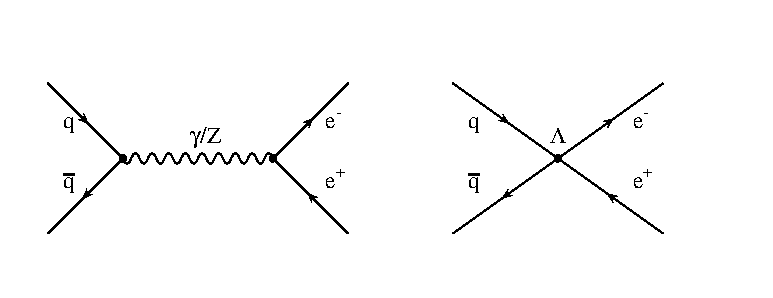
\includegraphics[width=0.8\linewidth]{images/compositeness.eps}
            \end{center}
            \caption{Feynman diagrams of a contact interaction (right) and the predominant background Drell-Yan production (left).}
            \label{fig:fd}
        \end{figure}

        Without knowing the intermediate process one can write a Lagrangian describing the new interaction; 

        \begin{equation}
            \mathcal{L} = \frac{g^{2}}{2\Lambda^{2}}
                [\eta_{LL} (\bar{\psi_{L}}\gamma_{\mu}\psi_{L}) (\bar{\psi_{L}}\gamma^{\mu}\psi_{L}) 
                + \eta_{RR} (\bar{\psi_{R}}\gamma_{\mu}\psi_{R}) (\bar{\psi_{R}}\gamma^{\mu}\psi_{R}) 
                + 2\eta_{LR} (\bar{\psi_{L}}\gamma_{\mu}\psi_{L}) (\bar{\psi_{R}}\gamma^{\mu}\psi_{R}) ]
        \end{equation}

        where $g$ is the coupling constant, $\Lambda$ is the energy scale of new physics and $\psi_{L}$ and $\psi_{R}$ are the left and right handed fermionic fields respectively. The sign of $\eta$ defines whether the new interaction interferes constructively ($\eta = -1$) or destructively ($\eta = +1$) with DY and is always unity. For previous analyses \cite{PhysRevLett.103.191803,PhysRevLett.96.211801,PhysRevD.87.015010} a benchmark model of just the Left-Left (LL) component has been used and defined by $\eta_{LL} = \pm~1$ and $\eta_{RR} = \eta_{LR} = 0$. Here however an investigation of each of the three parameters is done individually. Both the LL and RR cases are expected to behave similarly however the LR case exhibits a different angular dependence than either of the other formalisms or the DY background. This difference is the primary reason for the inclusion of the angular part of this analysis found later. The discriminating variables used are therefore dilepton invariant mass and cosine of the decay angle $\theta^{*}$. The angle $\theta^{*}$ is defined in the Collins-Soper frame \cite{PhysRevD.16.2219} which is defined with the $x$-axis perpendicular to the incoming parton momentum frame and the $z$-axis bisecting the angle between the two incoming parton momenta. Since the incoming parton information is understandably unavailable the $z$-axis is taken as the direction of the incoming quark (as opposed to anti-quark) obtained from the boost in to the dilepton frame. The angle $\theta^{*}$ is then defined as the angle between this $z$-axis and the momentum of the outgoing negatively charged lepton (or electron in this analysis).

        Figure \ref{fig:theoryAFB} shows the difference expected between the LR CI models and DY background from a truth Monte-Carlo study. The variables used are $A_{FB}$ and dilepton invariant mass where $A_{FB}$ is the forward-backwards asymmetry defined in relation to cos$\theta^{*}$ as;

        \begin{equation}
            A_{FB} = 
                \frac{N_{F} - N_{B}}{N_{F} + N_{B}}
            \label{eq:AFB}
        \end{equation}

        where $N_{F}$ and $N_{B}$ are number of events found with cos$\theta^{*}$ greater than 0 and less than 0 respectively.
        
        \begin{figure}[h]
            \begin{center}
            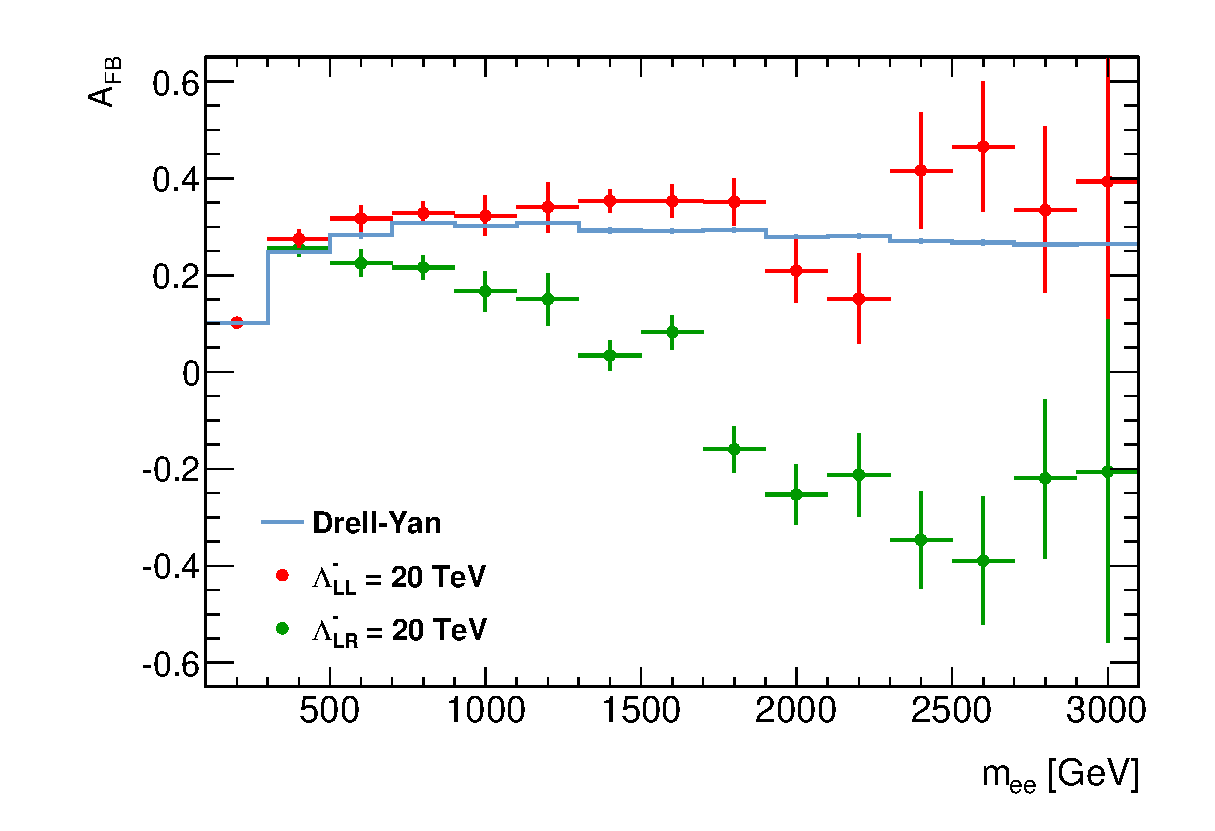
\includegraphics[width=0.8\linewidth]{images/AFB_MC.eps}
            \end{center}
            \caption{MC truth level comparison between the forward backwards asymmetry of DY and and of a CI LR signal.}
            \label{fig:theoryAFB}
        \end{figure}

        A differential cross section for this interaction, $q\bar{q} \rightarrow \ell^{-}\ell^{+}$ ($qq\ell\ell$), is given by

        \begin{equation}
            \frac{d\sigma}{dm_{\ell\ell}} = 
                \frac{d\sigma_{DY}}{dm_{\ell\ell}} 
                - \eta\frac{F_{I}}{\Lambda^{2}} 
                + \frac{F_{C}}{\Lambda^{4}},
            \label{eq:DiffCross}
        \end{equation}

        where $m_{\ell\ell}$ is the dilepton mass and $\Lambda$ is the scale of the new physics. In the case of quark/lepton compositness $\Lambda$ refers to the point at which fermions stop being bound as SM quarks and leptons. $F_{I}$ and $F_{C}$ define the interference DY-CI term and the pure CI term respectively. The scale of the interference and pure term vary with both the dilepton invariant mass as well as the scale of new physics $\Lambda$.

        Experimentally this interaction would be seen as a deviation from the Standard Model (SM) Drell-Yan (DY)($q\bar{q}~\rightarrow~\gamma/Z~\rightarrow~\ell^{+}\ell^{-}$) dilepton mass spectrum as seen in Fig. \ref{fig:theoryInvMass}). 

        \begin{figure}[h]
            \begin{center}
            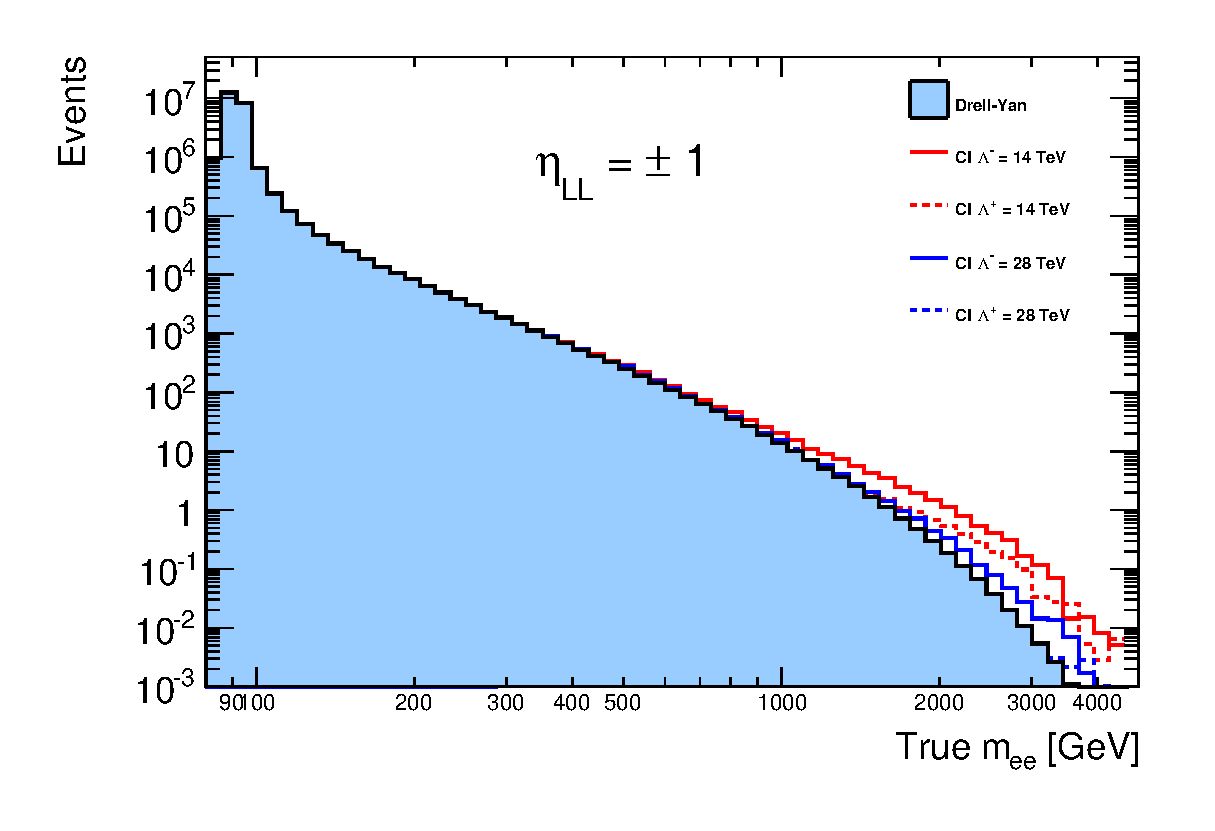
\includegraphics[width=0.8\linewidth]{images/truth_mass_LL.eps}
            \end{center}
            \caption{MC truth level comparison between DY spectrum with and without CI signal.}
            \label{fig:theoryInvMass}
        \end{figure}

    

    \subsection{ADD Theory}
        The large extra spacial dimensions theory described by Arkani-Hamed, Dimopoulos, and Dvali (or ADD theory) \cite{ArkaniHamed:1998rs} predicts a Graviton producing a non-resonant excess in the dilepton mass spectrum. The ADD theory describes a graviton that propagates the extra dimensions and acquires closely backed Kaluza-Klein (KK) modes that show as a broad excess above the SM background. 
        The ADD model was originally proposed to solve the hierarchy problem and bring the energy scale associated with gravity (the Planck scale M$_{Pl}$ ~ $10^{16}$ TeV) down to the level of electroweak energy scale (M$_{EM}$~ $10^{-1}$). This is achieved with the introduction of $n$ additional compactified spacial dimensions with radius $R$. This then gives a new scale in the 4+$n$ dimensional space, M$_{D}$, which is related to the Planck scale by M$_{Pl}$ = M$_{D}^{n+2}R^{n}$. If both the radius of the extra dimensions $R$ and and number $n$ are large enough this solves the hierarchy problem by bringing M$_{D}$ down to the level of M$_{EM}$.
        The Graviton is the only propagator in these extra $n$ dimensions with each dimension resulting in a new KK mass splitting of the mass peak. The mass splitting occurs with an interval of $1/R$ and since $R$ is required to be large by the theory this pushes the mass splitting together causing a continuous peak like structure analogous to a non-resonant excess. This sum over these virtual KK modes has to be regularised by an ``ultra violet'' cutoff ($\Lambda_{T}$) and it is convention to equate this cutoff to the onset of Quantum Gravity (M$_{S}$) only bellow which the theory is valid. This scale M$_{S}$ is used as the scale of physics for the ADD theory which is a low energy effective theory bellow this scale. This scale can be related to the new $n$ dimensional Planck scale (M$_{D}$) by;

        \begin{equation}
            M_{S} = 2~\sqrt{\pi}\left[{\Gamma (n/2)}\right]^{1/(n+2)}M_{D}
            \label{eq:gravScale}
        \end{equation}

        where $\Gamma$ is the decay width. Bellow the scale M$_{S}$ virtual Graviton exchange would lead to a broad excess over the SM Drell-Yan dileption mass spectrum. 
        The total differential cross-section for the dilepton SM DY and virtual Graviton exchange is then;

        \begin{equation}
            \frac{d\sigma}{dm_{\ell\ell}} =
                \frac{d\sigma_{DY}}{dm_{\ell\ell}} +
                \mathcal{F}\frac{F_{I}}{M_{S}^{4}} +
                \mathcal{F}^{2}\frac{F_{G}}{M_{S}^{8}}
            \label{eq:ADDcs}
        \end{equation}

        where $\sigma_{DY}$ is the SM DY cross-section, $F_{I}$ and $F_{G}$ are the Graviton-DY interactions term and pure virtual Graviton exchange term respectively while $\mathcal{F}$ is a formalism dependent parameter and also dimensionless. 
        Three formalisms are commonly used to describe ADD theory, these are Giudice, Rattazzi, and Wells (GRW) \cite{Giudice:1998ck}, Han, Lykken, and Zhang (HLZ) \cite{PhysRevD.59.105006} and Hewett \cite{PhysRevLett.82.4765}. Defining $\mathcal{F}$ these formalisms alter the cross-section of virtual Graviton exchange with HLZ depending on the number of extra dimensions, $n$, introduced by the ADD theory. All three formalisms are detailed in Eq. \ref{eq:ADDF}

        \begin{equation}
            \begin{aligned}
                \mathcal{F}~=&~1,   \quad &\text{(GRW)} \\
                \mathcal{F}~=&~  \left\{ 
                    \begin{array}{l l}
                        \log{(\frac{M_{S}^{2}}{m_{\ell\ell}^{2}})},      \quad & (n = 2) \\
                        \frac{2}{n-2},                                   \quad & (n > 2)
                    \end{array} \right.,  \quad &\text{(HLZ)}  \\
                \mathcal{F}~=&~\frac{2\lambda}{\pi}~=~\frac{\pm2}{\pi},     \quad &\text{(Hewett)}
            \end{aligned}
            \label{eq:ADDF}
        \end{equation}

        Of note the variable $\lambda$ found in the Hewett formalism defines the constructive or destructive nature of the gravitational interaction with the SM DY processes. $\lambda$ is always of order unity with +1 and -1 being constructive and destructive respectively.
        The GRW and HLZ with n = 2 are the two formalisms explicitly searched for in this analysis with a conversion of limits done to asses the other formalisms in the Statistical Analysis chapter.

        Experimentally this interaction would be seen as a deviation from the SM DY ($q\bar{q}~\rightarrow~\gamma/Z~\rightarrow~\ell^{-}\ell^{+}$) dilepton mass spectrum but with a cut-off where quantum gravity is assumed take effect. This can be seen in Fig. \ref{fig:theoryInvMassADD}. It is important to note that no angular difference in the virtual graviton decay is expected from that of SM DY, therefore ADD is only searched for in the dilepton mass spectrum.

        \begin{figure}[h]
            \begin{center}
            %\includegraphics[scale=0.3]{}
            \end{center}
            \caption{MC truth level comparison between DY spectrum with and without ADD signal.}
            \label{fig:theoryInvMassADD}
        \end{figure}



\section{Past Searches}

    {\bf Contact Interaction}\\
        Several previous CI analyses have been done at hadron colliders including the LHC \cite{PhysRevD.87.015010,ATLAS:2012pu,PhysRevD.87.032001,PhysRevD.87.052017} and the Tevitron \cite{PhysRevLett.103.191803,PhysRevLett.96.211801,PhysRevLett.87.231803,PhysRevLett.82.4769,PhysRevLett.79.2198}. Searches were also performed at the electron-proton collider HERA \cite{Chekanov200423,Adloff200335}, previous lepton colliders \cite{Abdallah2009.60.1,Schael2007.49.411,Abdallah2006.45.589,Abbiendi2004.33.173,Acciarri200081} and neutrino scattering experiments \cite{}. Of the results comparable to this analysis searching for $qq\ell\ell$ Contact Interactions in the absence of signal the highest limits set on the scale of new physics $\Lambda$ come from the previous ATLAS analysis \cite{PhysRevD.87.015010} detailed in appendix A. This analysis set a limit of $\Lambda$ $>$ 12.7 TeV and $\Lambda$ $>$ 9.63 TeV for the dilepton LL CI model for constructive and destructive interference respectively. The limits obtained for the electron channel for comparison to this analysis were $\Lambda$ $>$ 11.6 TeV for constructive and $\Lambda$ $>$ 8.76 TeV for destructive interference. \\


    {\bf ADD}\\
        The highest dilepton ADD limits set on the formalism normally used as a bench mark, GRW, are that of the previous ATLAS analysis \cite{PhysRevD.87.015010} discussed in Appendix A which sets a limit of 3.0 TeV on the scale of new physics (M$_{S}$). Preliminary results from CMS on the LHC data set used in this analysis do however show higher limits but are not yet published. Other previous analyses have also been carried out searching for large extra dimensions with the ADD model. These analyses have come from the LHC \cite{}, from the Tevatron \cite{}, as well as from electron-proton collider HERA \cite{} and electron-positron collider LEP \cite{}. 









\newpage
\chapter{Experiment}

	This chapter will explore the ATLAS experiment in order to explain how data specific to this analysis is obtained. First however is a discussion of the Large Hadron Collider which supplies the ATLAS experiment with proton collisions.

\section{The Large Hadron Collider}

	\begin{figure}[h!]
        \begin{center}
            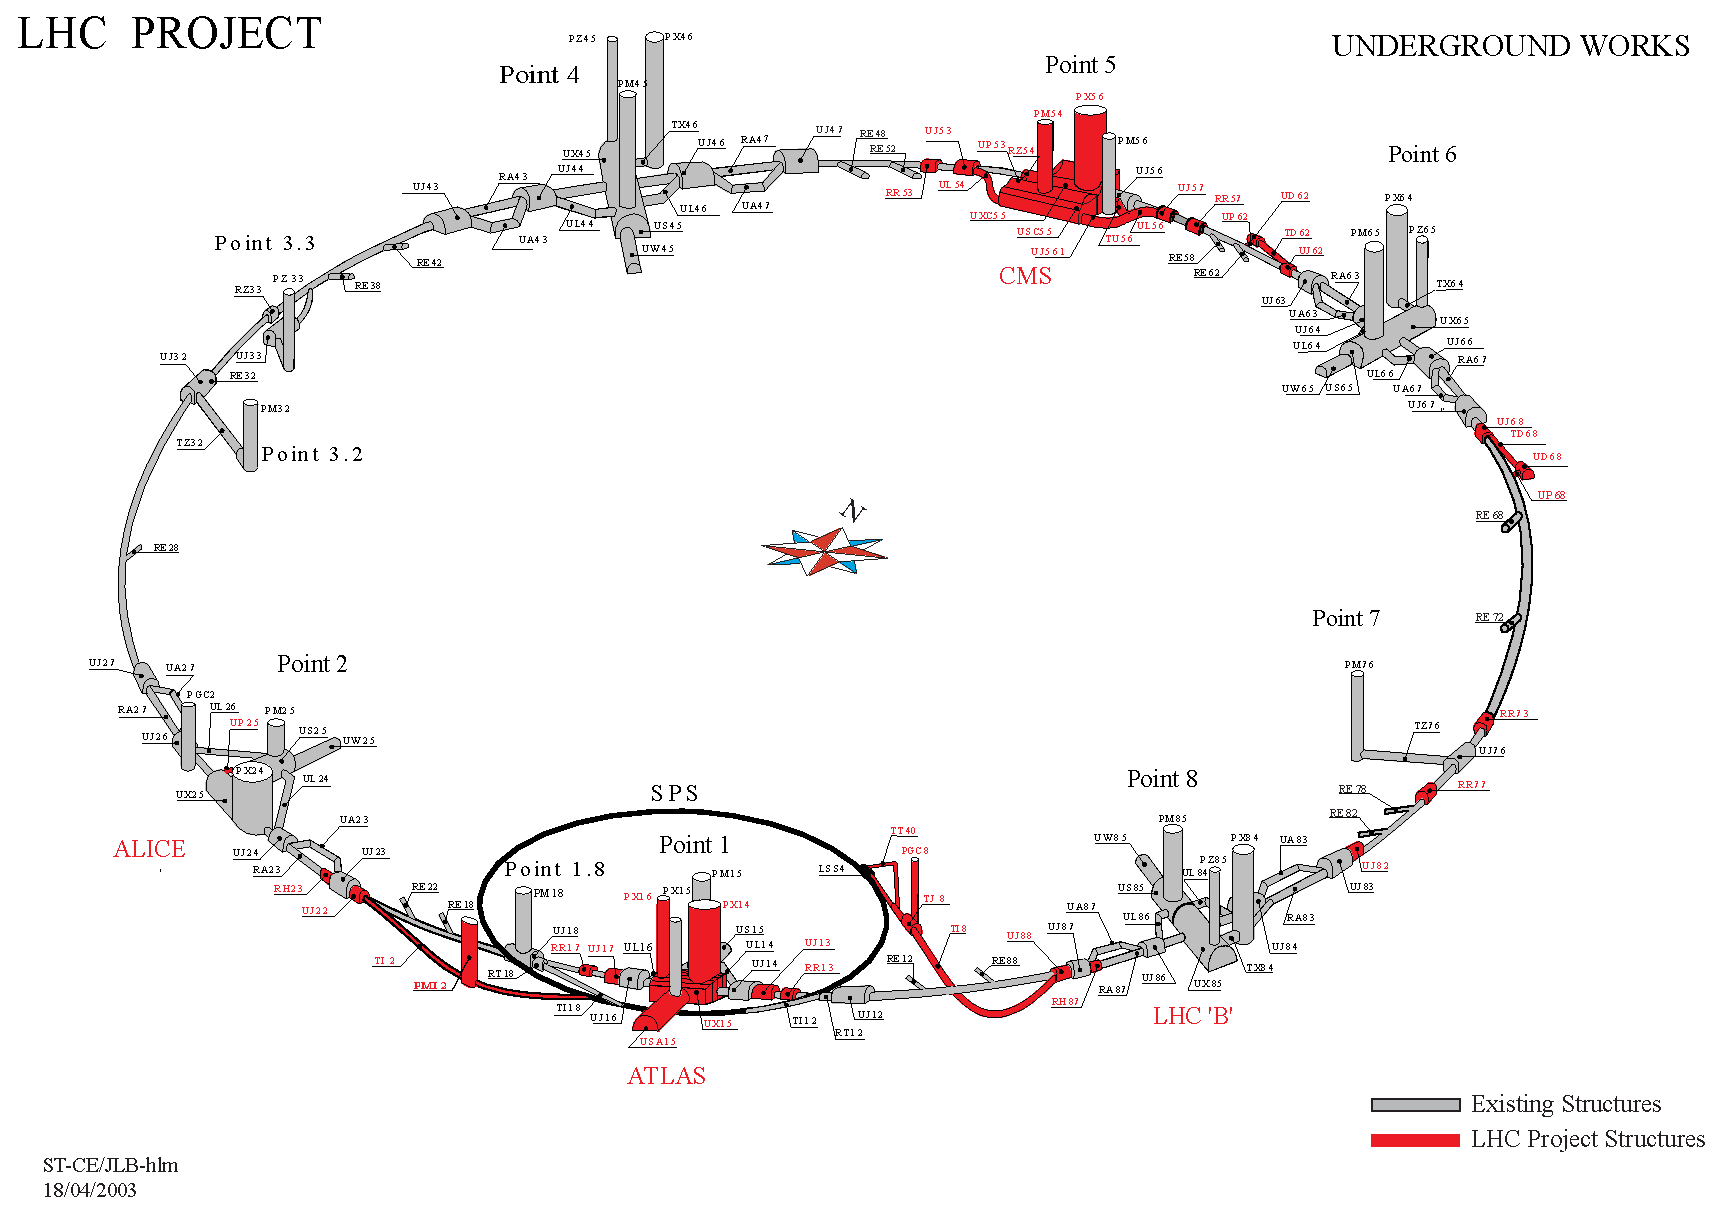
\includegraphics[scale=0.6]{images/LHCUnder.eps}
        \end{center}
        \caption{Schematic of LHC tunnel with all its caverns showing those added in preparation for the LHC. This shows the position of the LHC's 4 main detectors and SPS ring \cite{1367-2630-9-9-335}.}
        \label{fig:experimentLHC}
    \end{figure}

	The Large Hadron Collider (LHC) \cite{Brüning:782076} is the largest and most powerful particle collider in the world with a circumference of $27$ km and design centre of mass collision energy of $14$ TeV. During the 2012 run the accelerator was run at a centre of mass energy of $8$ TeV while providing an integrated luminosity of just above $20~fb^{-1}$ throughout the year to its two general purpose experiments, CMS and ATLAS, that latter of which provided data for this analysis.
	
	The LHC itself is built in the same tunnel (see fig. \ref{fig:experimentLHC}) as was used by the Large Lepton-Positron (LEP) collider. Based at CERN (Centre of European Nuclear Research) the $27$ km tunnel is between $50$ to $175$ m underground and like CERN itself crosses the French-Swiss border just outside Geneva. Construction of the LHC started in 2001 after the LEP collider was decommissioned and dismantled with excavation of the caverns for the LHC's four main experiments starting slightly before in 1998. 
	The LHC is a synchrotron machine requiring 1,232 super-conducting Niobium-Titanium dipole magnets each providing an $8.33$ T magnetic field to direct the proton beams around its loop and an additional 392 quadrupole magnets of the same type to focus the beams for the collision points. The super conducting magnets operate at $1.9$ K with the whole accelerator requiring 96 tonnes of liquid helium to remain cooled.\\

	%%%%%%%%%%%%%%%Fill in!!!!!!!!!!!!!!!!!!!!!!!!
	For the 2012 run used in this analysis the LHC ran with xxxx proton bunches travelling in each direction which were accelerated around the LHC with an interval of 50 ns between bunches and with each bunch composed of xxxx protons. These run conditions gave an instantaneous luminosity of xxxx at the start of a run which slowly degraded during a run as protons collided. % design?
	%%%%%%%%%%%%%%%Fill in!!!!!!!!!!!!!!!!!!!!!!!!

	However the LHC can not run in isolation to provide beams for its 4 main experiments, instead it is the last and newest accelerator in a chain of accelerators which extract protons from a hydrogen canister with little to no momentum and inject them in to the LHC as a 450 GeV beam.
	The proton source is a device called a Duoplasmatron which injects hydrogen gas in to a strong electric field striping electrons from their nuclei. The remaining protons are injected in to Linac 2, a linear accelerator which accelerates them to an energy of $50$ MeV. The BOOSTER or Proton Synchrotron Booster (PBS) comes next in the chain and accelerates protons from $50$ MeV to $1.4$ GeV to be injected in to the main Proton Synchrotron (PS). The PS accelerates protons up to an energy of $25$ GeV and again injects them in to another accelerator, the Super Proton Synchrotron (SPS). The SPS (seen in fig. \ref{fig:experimentLHC}) is the final stage before injection in to the LHC ring and pushes protons to an energy of $450$ GeV. Protons from the SPS then get injected in to the LHC in both counter revolving directions and accelerated to their final collision energy. For the data used in the analysis that follows (the 2012 data run) the final proton beam energy is $4$ TeV giving a final centre of mass collision energy of $8$ TeV.

	Four collision points exist around the circumference of the LHC providing collisions to the four main experiments (see fig. \ref{fig:experimentLHC}); ATLAS (A Toroidal LHC Apparatus), CMS (Compact Muon Solenoid), ALICE (A Large Ion Collider Experiment) and LHCb (Large Hadron Collider beauty). ATLAS and CMS are both general purpose experiments designed to look for a variety of physics. ALICE is designed specifically to study quark-gluon plasma in heavy ion collisions scheduled for the end of each LHC run period while LHCb looks for beauty mesons in searches for CP-violation.
	There are also three additional LHC detectors in various stages of deployment without their own collision points; TOTEM (Total Elastic and diffractive cross section Measurement), LHCf (LHC forward) and MoEDAL (Monopole and Exotics Detector at the LHC) which measure separate beam properties. TOTEM shares CMS's collision point aiming to measure the proton cross-section very accurately while LHCf shares ATLAS's collision point measuring the very forward region of collision with the hope of investigating the source of ultra-high-energy cosmic rays. MoEDAL shares a cavern with LHCb and is targeted to search for magnetic monopoles and other highly ionising stable massive particles.


%\newpage

\section{ATLAS - A Toroidal LHC Apparatus}

	\begin{figure}[h]
		\begin{center}
			\includegraphics[scale=0.1]{images/ATLAS_SE_Corrected7.eps}
		\end{center}
		\caption{Cut-away view of the ATLAS detector. The dimensions of the detector are 25 m in height and 44 m in length. The overall weight of the detector is approximately 7000 tonnes \cite{Aad:1129811}.}
		\label{fig:ATLAS_cutaway}
	\end{figure}


	The ATLAS detector \cite{Aad:1129811} sits \SI{100}{\m} underground just over the road from the main CERN site and at \SI{45}{\m} long, \SI{25}{\m} in diameter and weighing over 7,000 tons is one of largest and most complex particle physics experiments in the world. The Detector itself can be divided in to four main subsystems and from the interaction point out they are; the inner detector (ID) or tracking detector, the calorimeters both Electro-Magnetic (EM) and hadronic (HCAL), the magnet system and the muon spectrometer (MS). There is also a small set of forward detectors, not detailed here, for accurate measurement of the integrated luminosity provided to ATLAS by the LHC named ALFA, LUCID and ZDC \cite{Aad:1129811}. 

	As a whole the detector has several different sets of coordinate systems some of which are used in analysis and some used primarily in detector design and placement. The first is z or the z-axis. This runs along the beam line through the centre of the detector with 0 existing at the very centre of the detector. x and y-axes do exist but are rarely needed as radial coordinates serve the purpose better. Here R is then the radial distance out from the beam line and $\phi$ is the angle perpendicular to R and z measuring the angle around the barrel of the detector. The last coordinate is $\theta$ measuring the angle off of the z-axis. This angle however isn't often used and in stead the angle $\eta$ or pseudorapidity is used. Defined in Eq. \ref{eq:eta} this quantity has the benefit of being invariant under transformation.

	\begin{equation}
		\eta~=~-\ln[\tan(\frac{\theta}{2})]
		\label{eq:eta}
	\end{equation}

	Broadly the detector is also divided in to the barrel region (cylinder surrounding the interaction point) and endcap regions (circles covering the ends of the barrel region) which use slightly different configurations and technology in order to cover a full range in $\eta$.
	Following is a description of each main subsystem while focusing particularly on both the Inner Detector and EM calorimeter as these are the important systems in identification of electrons used for this analysis. This section heavily uses the ATLAS technical design report \cite{Aad:1129811} throughout. 


	%(- structured to hold it up?)

	\begin {table}[h]
	\begin{center}
	\begin{tabular}{ | l | c | c | c | } 
		\hline
		Detector component & Required resolution & \multicolumn{2}{c|}{$\eta$ coverage} \\
		 & & Measurement & Trigger \\
    	\hline\hline
    	Inner Detector & $\sigma_{p_{T}}/p_{T}~~=~0.05\%~p_{T}~\oplus~1\%$ & $|\eta|<2.5$ & N.A \\
    	\hline
    	EM calorimetry & $\sigma_{E}/E~=~10\%/\sqrt{E}~\oplus~0.7\%$ & $|\eta|<3.2$ & $|\eta|<2.5$ \\
    	\hline
    	Hadronic calorimetry (jets) &  &  &  \\
    	~~~barrel and end-cap & $\sigma_{E}/E~=~50\%/\sqrt{E}~\oplus~3\%$ & $|\eta|<3.2$ & $|\eta|<3.2$ \\
    	~~~forward  & $\sigma_{E}/E~=~100\%/\sqrt{E}~\oplus~10\%$ & $3.1<|\eta|<4.9$ & $3.1<|\eta|<4.9$ \\
    	\hline
    	Muon spectrometer & $\sigma_{p_{T}}/p_{T} =10\%$ at $p_{T} = 1$ TeV & $|\eta|<2.7$ & $|\eta|<2.4$ \\
    	\hline
  	\end{tabular}
  	\label{tab:det_res}
  	\caption{Table showing detector components resolution requirements and $\eta$ ranges for triggering and readout \cite{Aad:1129811}.}
  	\end{center}
	\end {table}

  	%(- table of eta range, no. layers, output channels of every part of ID and CAL's)



	\subsection{Inner Detector}

		\begin{figure}[h]
			\begin{center}
				\includegraphics[scale=0.175]{images/ID_newTRT_d3.eps}
			\end{center}
			\caption{Cut-away view of the ATLAS inner detector \cite{Aad:1129811}.}
			\label{fig:ATLAS_inner}
		\end{figure}

		The Inner Detector is ATLAS's main tracking detector which is fitted closest to the interaction point. A tracking detector is needed to trace charged particles from the interaction point out to the calorimetry system and give two bits of information; a charged particle's position to match with the calorimeters (or Muon Spectrometer in the case of muons) and when a magnetic field is present an estimate of a particle's momentum to compare with the calorimeter obtained from the radius of its curve. The  ATLAS tracking system is composed of three different tracking technologies in order going out from the collision point; the Pixel Detector (PD), the Semiconductor Tracker (SCT) and the Transition Radiation Tracker (TRT). The Inner Detector was designed to precisely measure charged tracks in the energy range 0.5 GeV - 150 GeV while complimenting the energy measurements of the calorimetry system. Covering a range of $|\eta|~<~2.5$ and full range in $\phi$ the Inner Detector with the help of the 2 T magnetic field imposed by the solenoid magnet (discussed bellow) boasts a momentum resolution of $\sigma_{p_{T}}/p_{T}~=~0.05\%~p_{T}~\oplus~1\%$ for charged tracks. In its design it was also important for the Inner Detector to be able to distinguish between multiple primary vertices at the collision point, referred to as pile-up, as well as secondary vertices from sources such as the hadronisation of b quarks. 
		%(-stats as to precision?)

		\begin{figure}[h]
			\begin{center}
				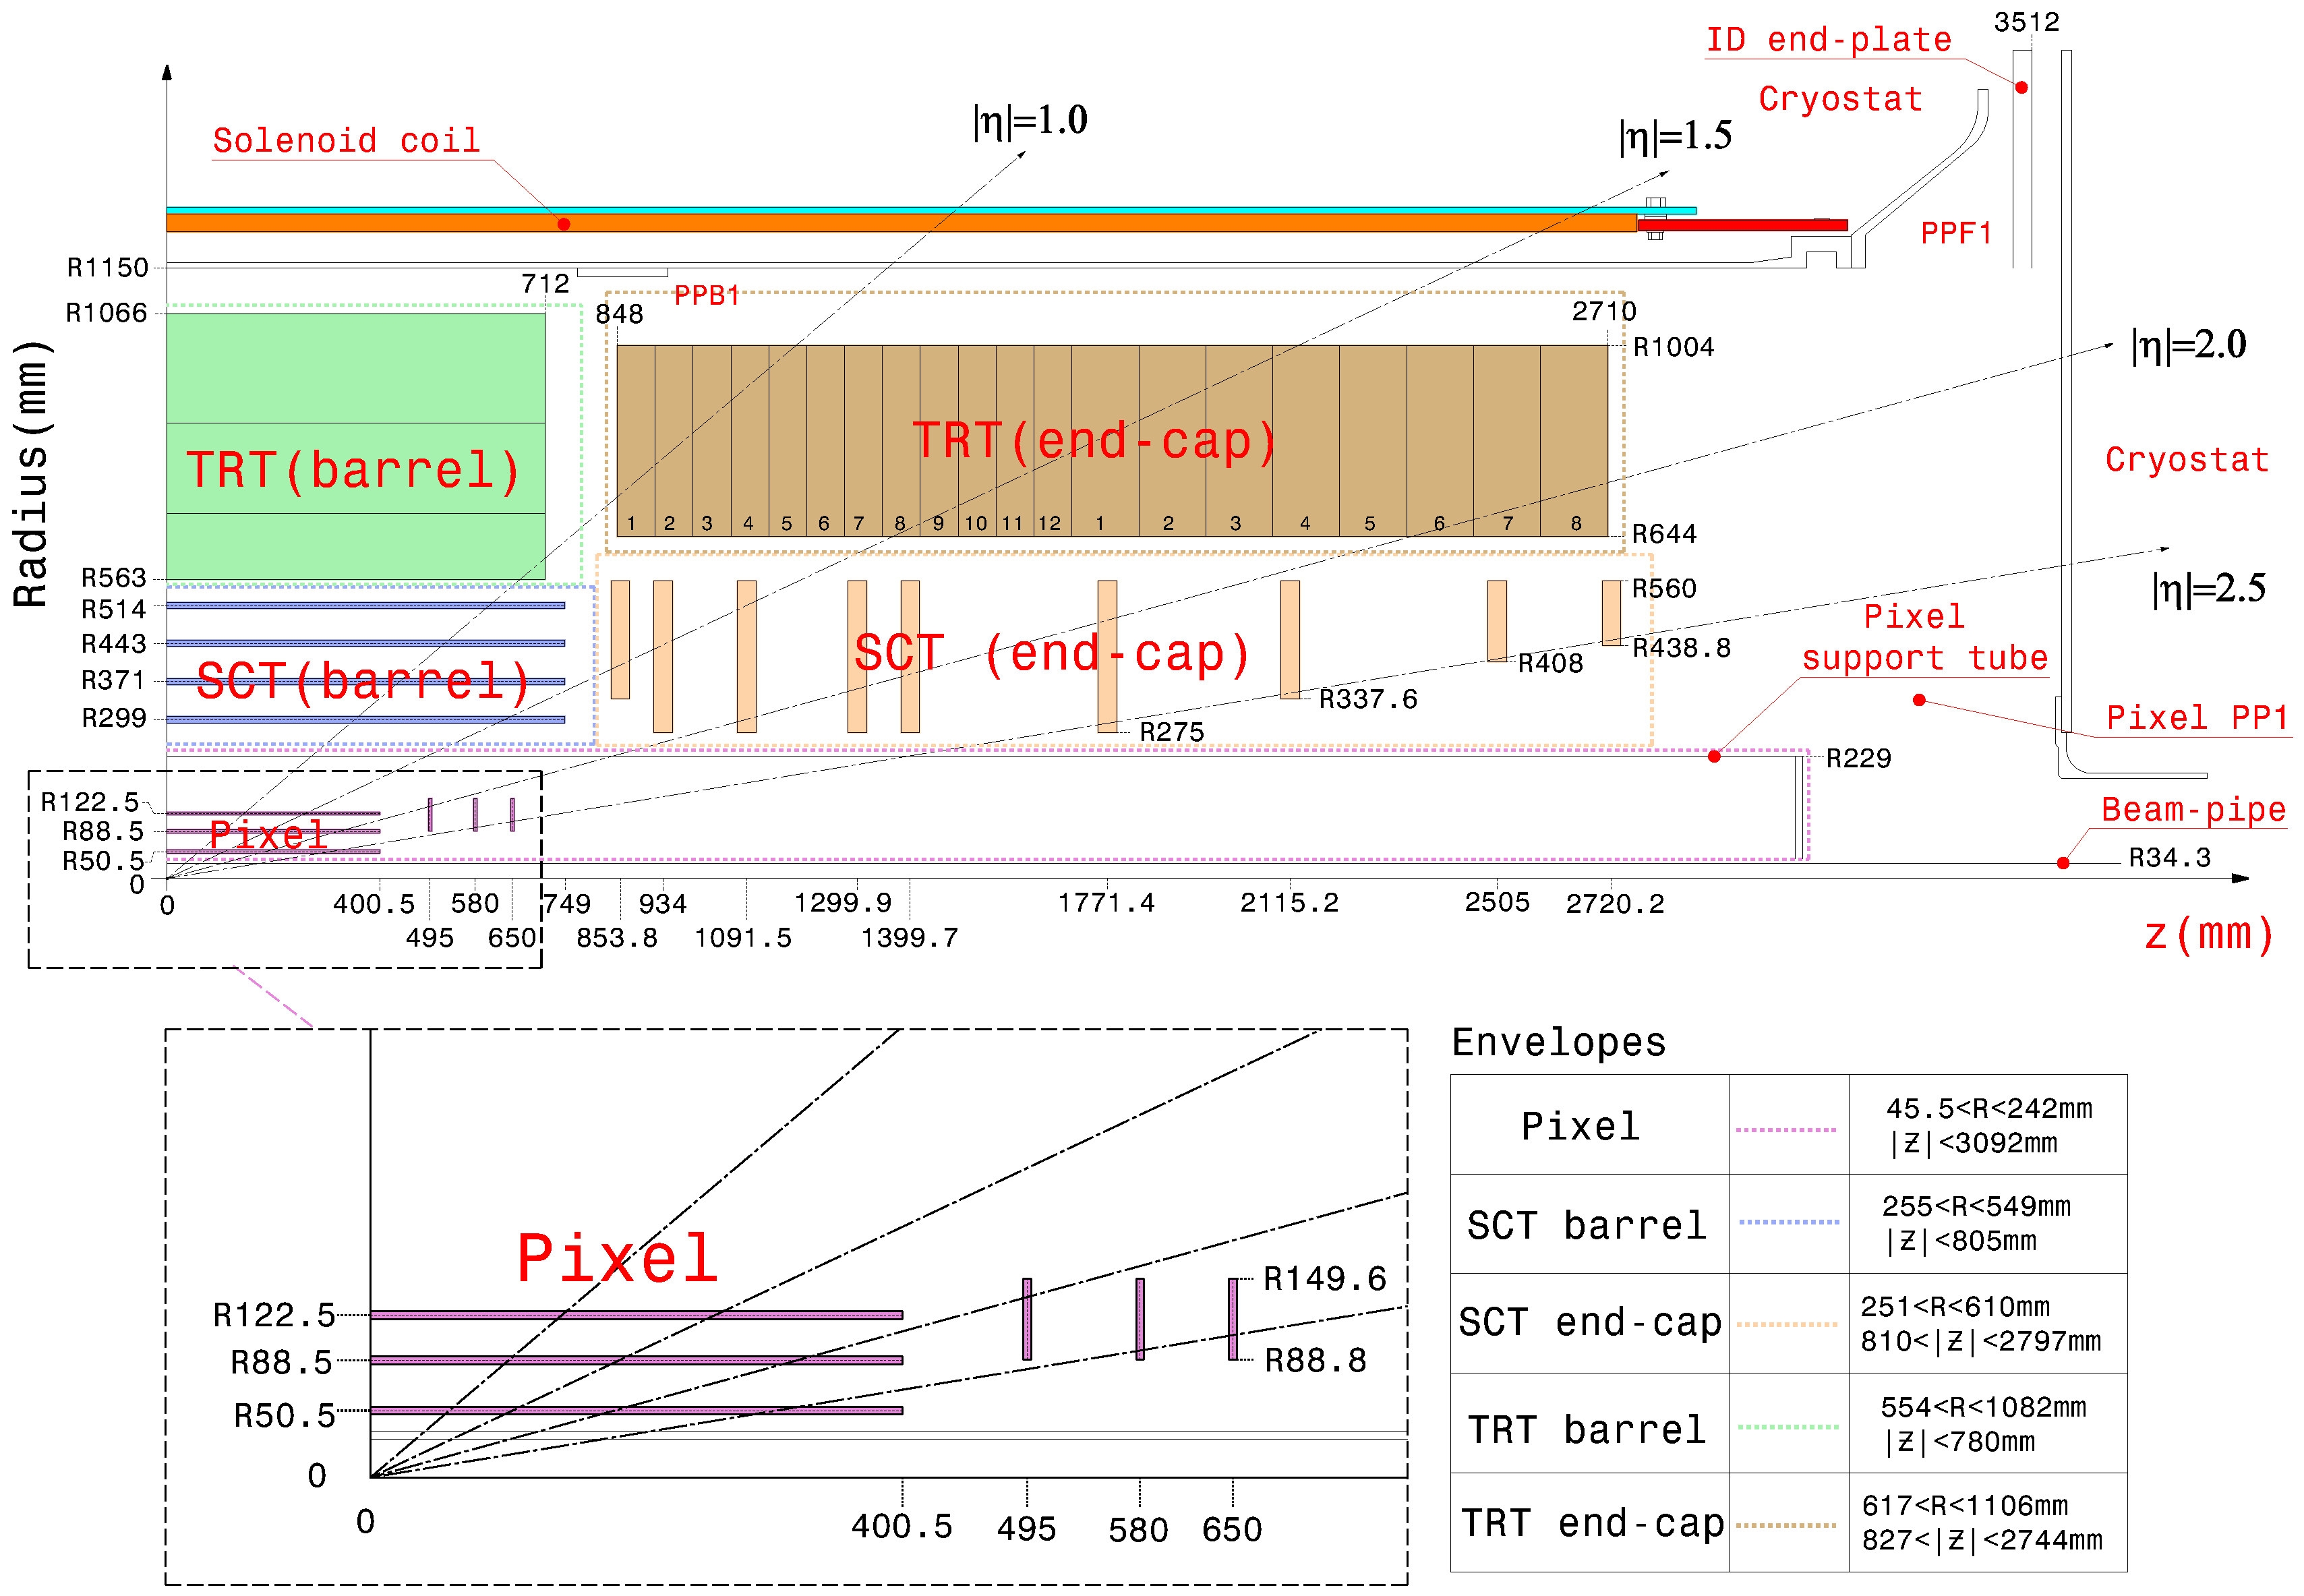
\includegraphics[scale=0.3]{images/FigID26-mod-011107.eps}
			\end{center}
			\caption{Plan view of a quarter-section of the ATLAS inner detector showing each of the major detector elements with its active dimensions and position is Z and R detector coordinates (envelopes) \cite{Aad:1129811}.}
			\label{fig:ATLAS_inner_config}
		\end{figure}



		\subsubsection*{Pixel Detector} 

		The Pixel Detector is the first layer and closest to the beam line consisting of three layers of silicon pixels. Because of its proximity to the beam line the pixel detector are designed to be heavily radiation hard and understood to the degree that its performance can be predicted over an extended period of radiation exposure. The Pixel Detector is made of a barrel and two endcaps composed of 1744 modules all together. \\
		%(- each module, no. pixels)
		%(- keep cool to avoid leakage current.)
		%(-read out channels?)


		\subsubsection*{Semiconductor Tracker}

		The SCT consists of the same technology as the PD but is organised in to 4 layers in the barrel region and 9 layers in each endcap. Due to the packed nature of these electronics cooling is important in this layer and so the sensors in each module are glued to each side of a thermally conductive spine that gives the SCT both structure and allows transport of heat out via the mounting point of each module keeping them at their operating temperature of \SI{-7}{\degreeCelsius}.\\
		%(-read out channels?)



		\subsubsection*{Transition Radiation Tracker}

		The TRT uses a completely different tracking technology to the rest of Inner Detector using straw detectors composed of 4 mm diameter polymide tubes each with a \SI{31}{\um} diameter gold plated Tungsten-Rhenium wire. Due to the small diameter of the straws the TRT can obtain the high read-out rate needed for experiments at the LHC. The barrel region consists of 50,000 of these straws with a readout at each end providing 100,000 readout channels. The endcaps contain another 320,000 straws only read out a one end giving the TRT a total of 420,000 channels. Each channel measures drift time giving a resolution of \SI{170}{\um} in each straw. The straws are filled with a high Xenon concentration (\ce{Xe}(70\%)\ce{CO2}(27\%)\ce{O2}(3\%)) of gas in order to detect electrons via radiated photons as they traverse the material between straws (-what is this material?). This is achieved by giving each straw two timing thresholds, the lower to discriminate tracking hits (direct hits) while the higher threshold discriminates transition radiation hits. \\ %discuss
		%(-eta ranges of barrel end cap.)
		%(-number of straw hits in each region) 
		



	\subsection{Calorimeters}

		\begin{figure}[h]
			\begin{center}
				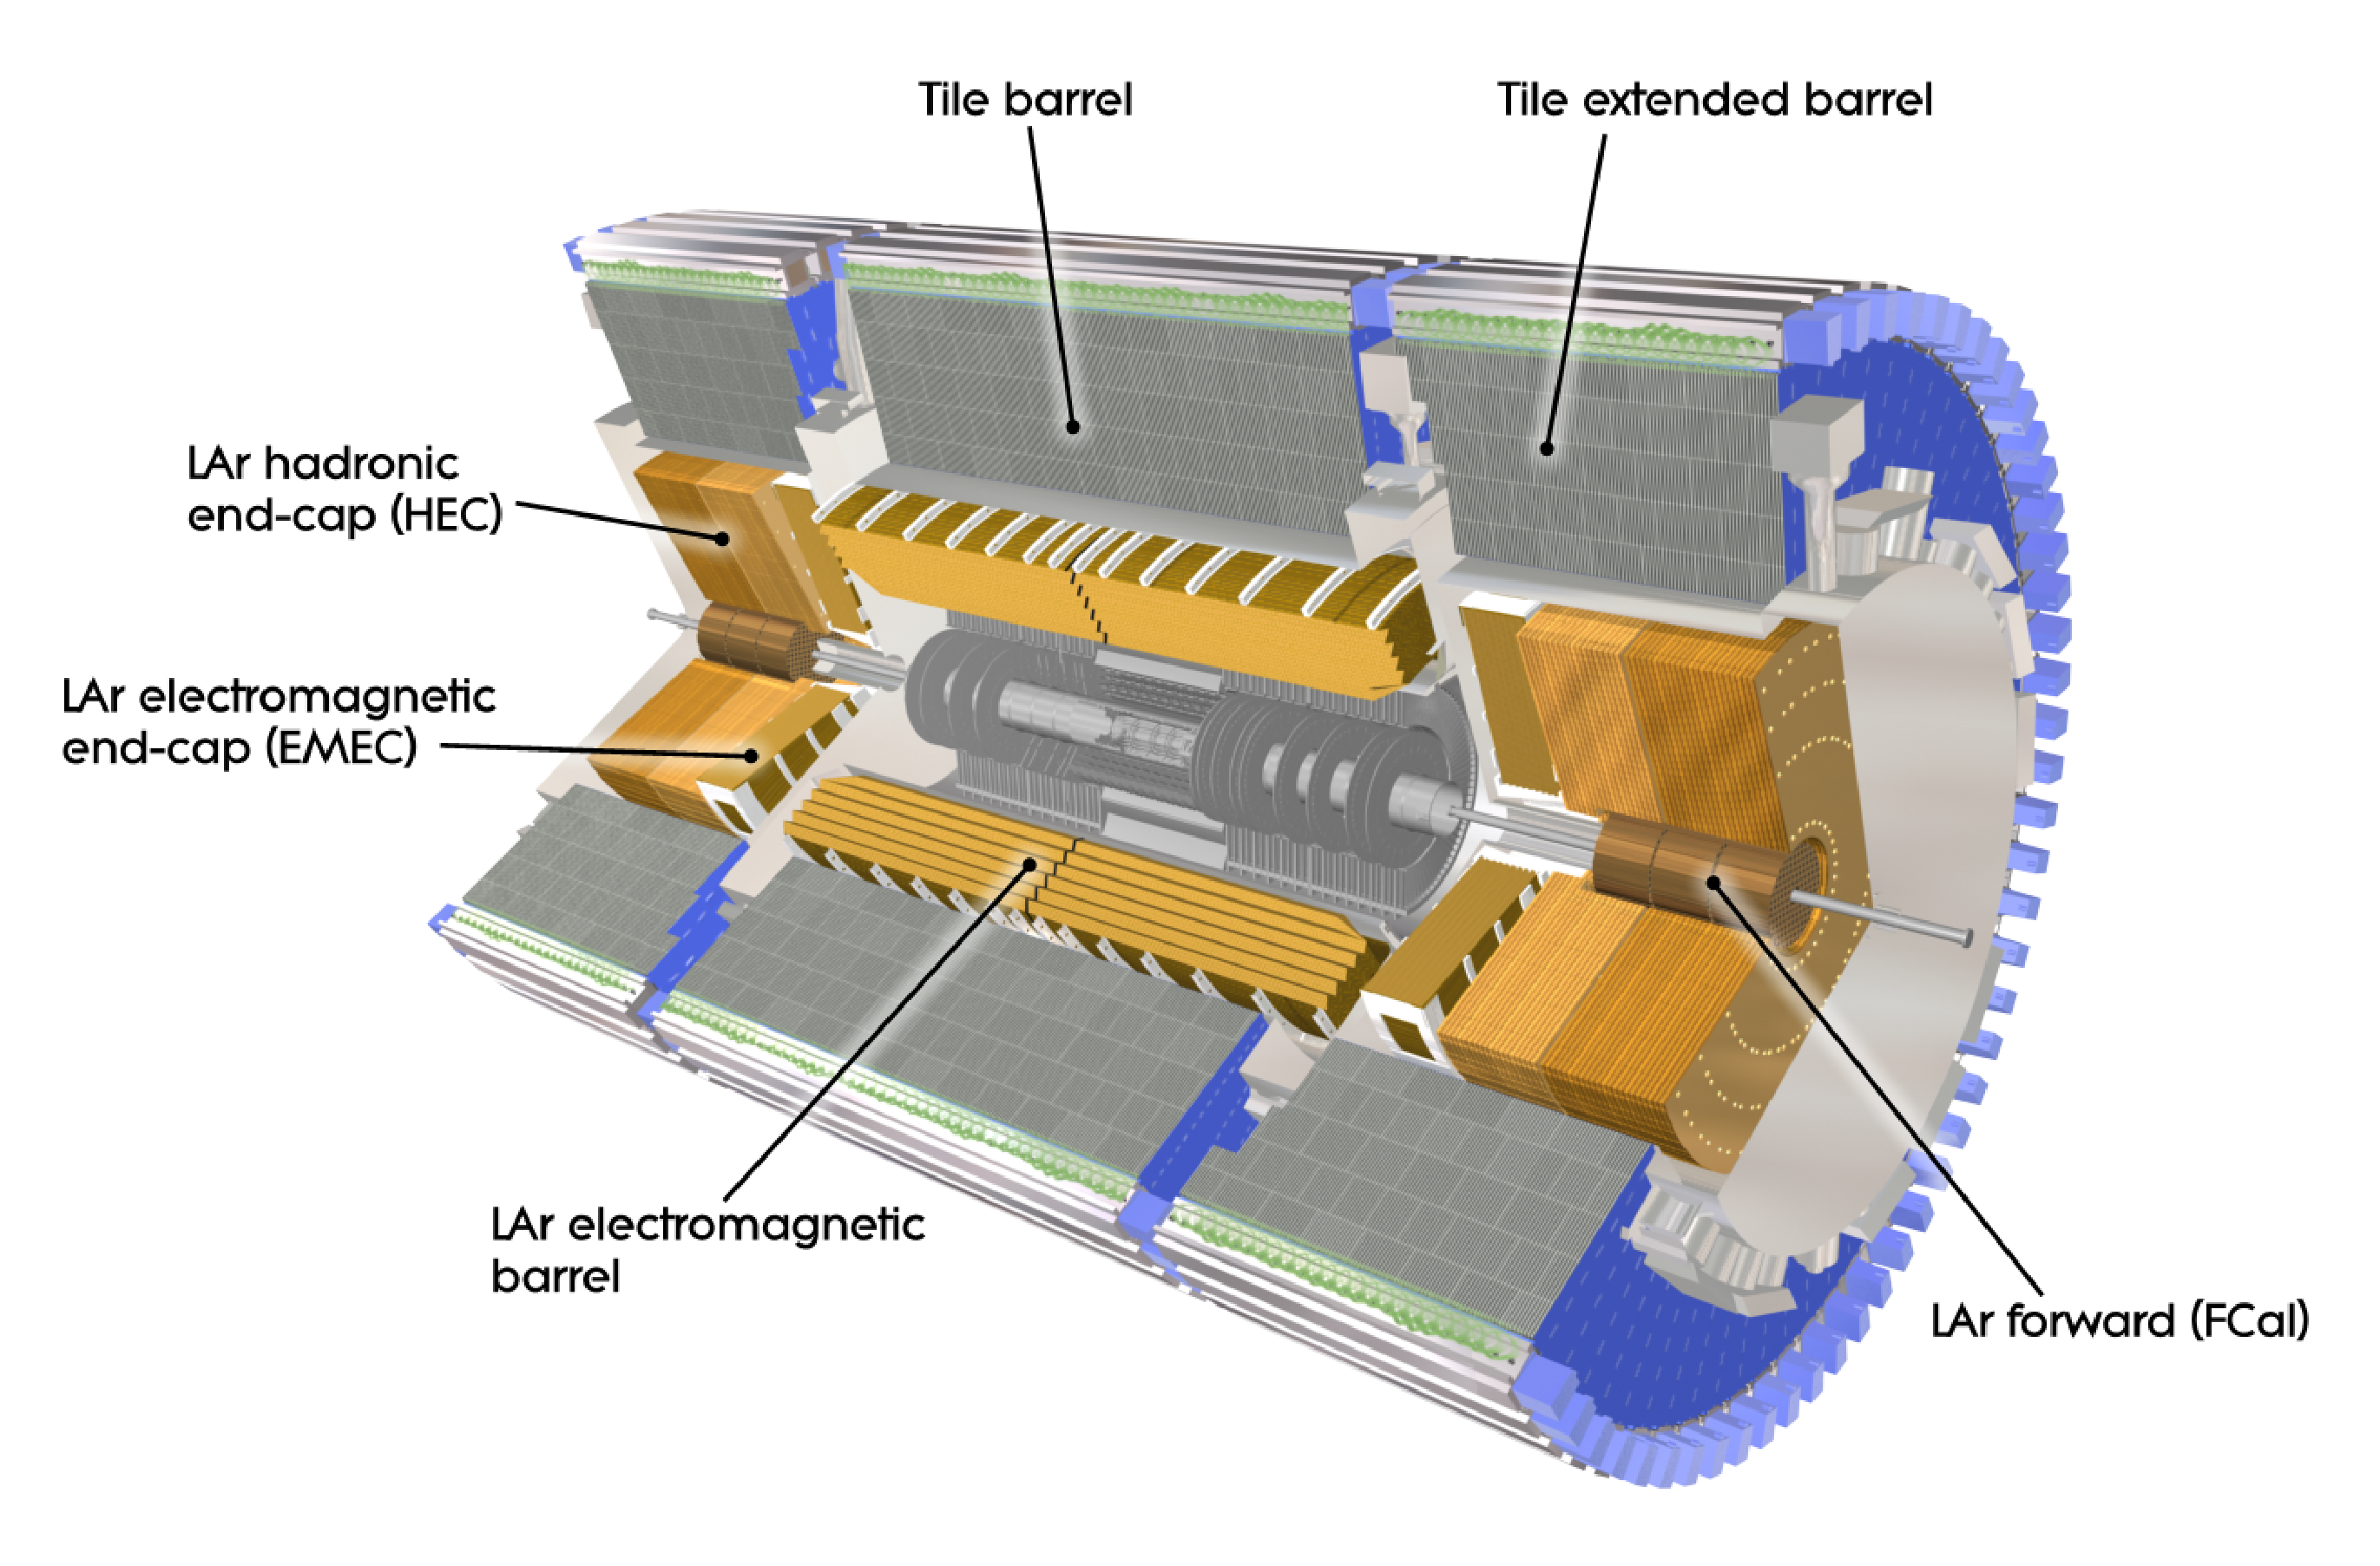
\includegraphics[scale=0.35]{images/Calorimeter_d3.eps}
			\end{center}
			\caption{Cut-away view of the ATLAS calorimeter system \cite{Aad:1129811}.}
			\label{fig:ATLAS_calo}
		\end{figure}

		While the Inner Detector only measures charged particles, the calorimeters measure both neutral and charged particles and are split in to two sections for particles with differing properties. The inner Electromagnetic Calorimeter is designed primarily to measure electrons and photons as well as pions while the outer Hadronic Calorimeter looks for hadrons such as neutrons and protons. In analyses the Hadronic Calorimeter is primarily used to look for jet objects (a collection of particles issuing from the decay of one mother particle). The primary method of identifying charged particles is to look for an associated track within the Inner Detector although the shape of the energy deposit in the calorimeters also helps with identification.

		%(- radiation thickness of detector)
		%(- prevent leakage in to next layer)


		\begin{figure}[h]
			\begin{center}
				\includegraphics[scale=0.5]{images/ITCconcept_new.eps}
			\end{center}
			\caption{Schematic of the transition region between the barrel and endcap cryostats \cite{Aad:1129811}.}
			\label{fig:ATLAS_calo_crack}
		\end{figure}


		\subsubsection*{Electromagnetic Calorimeter}

		The Electromagnetic Calorimeter (ECAL) is designed to fully stop all electromagnetic showers within its volume. Split in to a barrel section and two endcaps the ECAL uses Liquid Argon (LAr) as a detecting medium with lead as the absorber. The lead is arranged in an accordion fashion (seen in *) to ensure consistent performance throughout $\phi$. In the barrel section a presampler of LAr type is found before the main calorimeter to correct later sub-detectors for dead material. The barrel contains three layers of LAr modules of decreasing size in towards the collision point in order to keep good position resolution. The endcap only contains two layers of modules with the the inner layer containing smaller modules for the same reason as the barrel region.\\

		%(- shape information and electons/photons/pions)
		%(- energy resolution)
		%(- forward calorimeters)

		\subsubsection*{Hadronic Calorimeter}

		The Hadronic Calorimeter is designed to stop all hadronic showers within its volume and consists of two parts, the Tile Calorimeter (HCAL) in the barrel and the LAr Hadronic Endcap (HEC). The HCAL is a tile calorimeter consisting of alternating layers of scintillator and steel as the active medium and absorber respectively. The HEC on the other hand uses the same technology as the ECAL with copper plates filled with LAr as the detecting medium. As the Hadronic Calorimeter sits directly behind the ECAL it is used selecting good electron candidates using hadronic isolation or the amount of leakage in to the HCAL from a electron shower in the ECAL.\\
		%(- eta ranges?)
		%(- forward calorimeters)
		


	\subsection{Magnet System}

		
		\begin{figure}[h]
			\begin{center}
				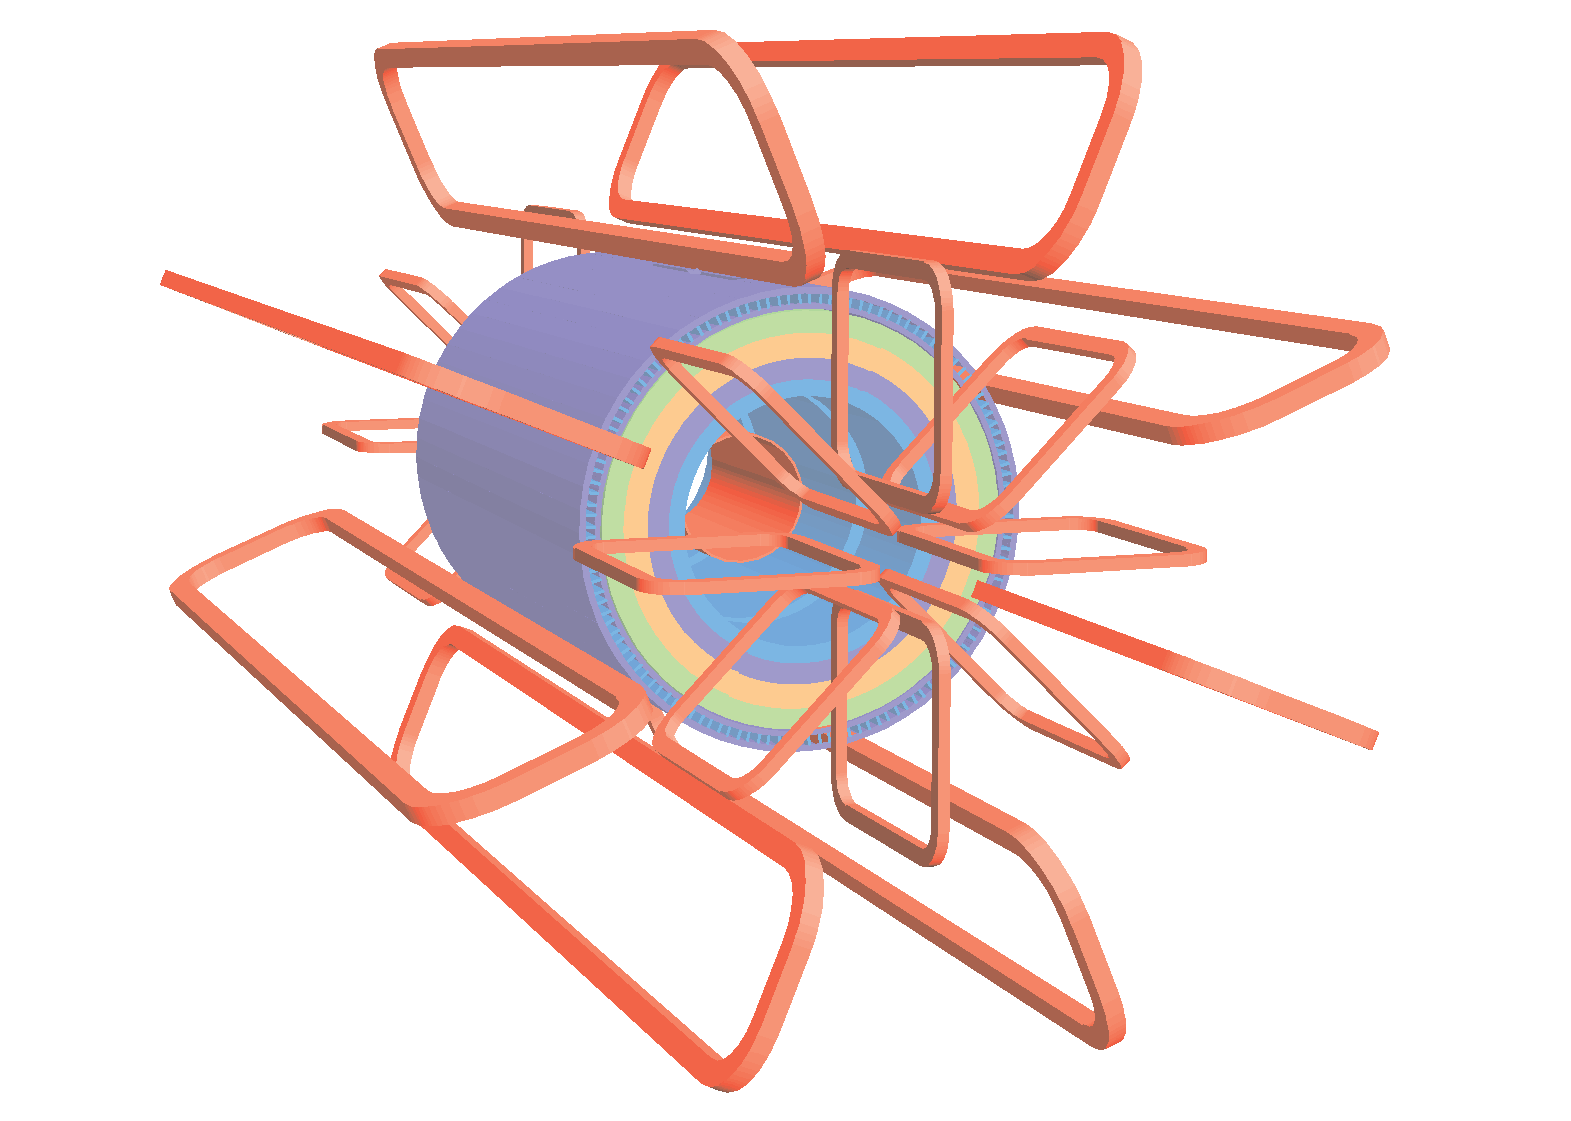
\includegraphics[scale=0.3]{images/ATLcoilGeom.eps}
				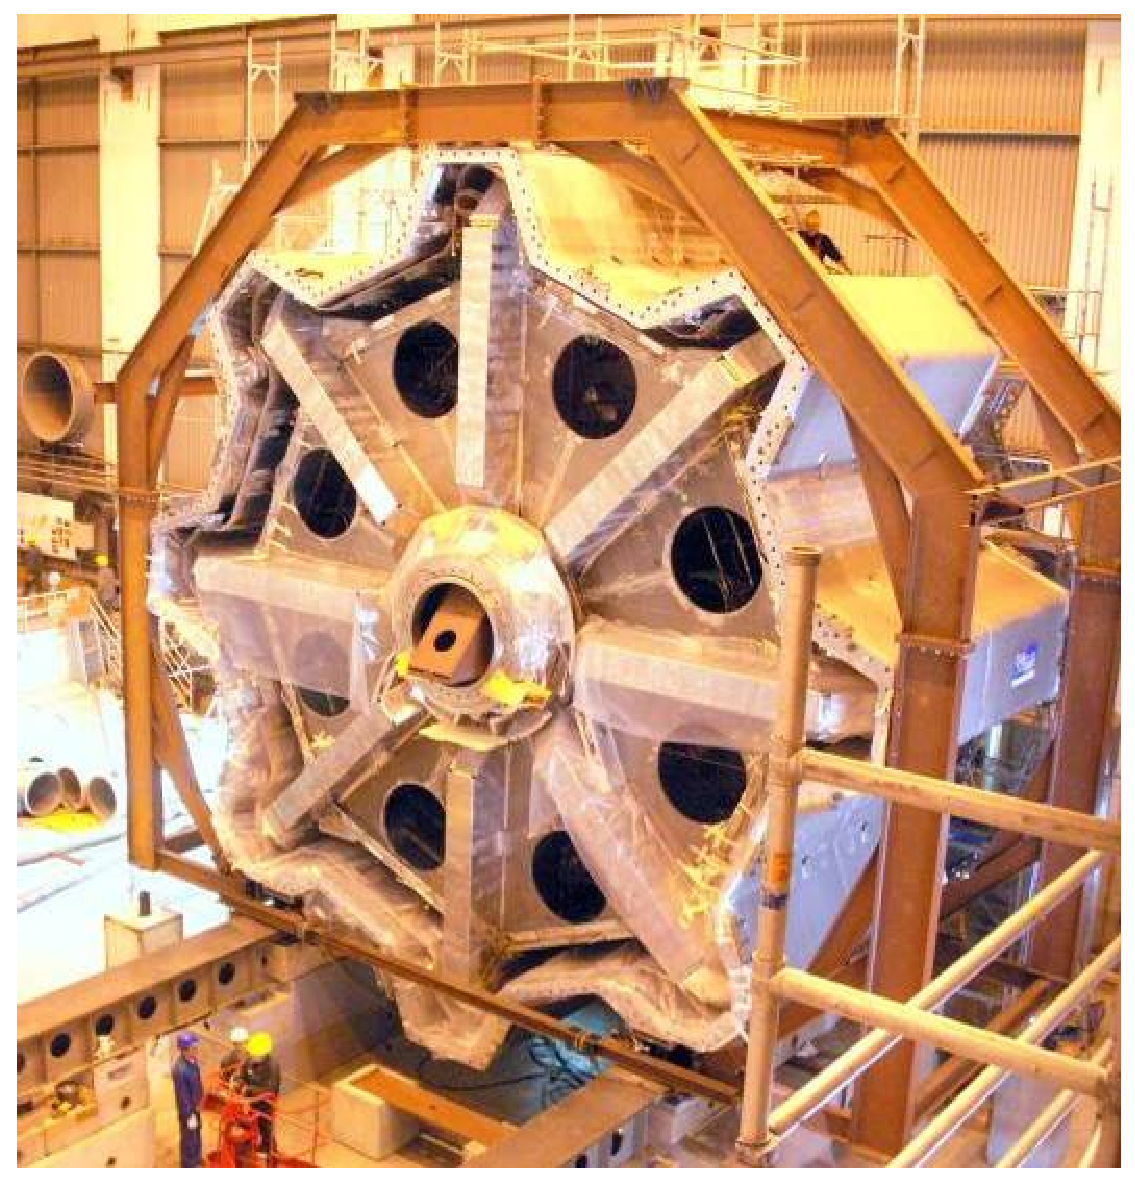
\includegraphics[scale=0.3]{images/desc5.eps}\\
				\includegraphics[scale=0.3]{images/desc6.eps}
			\end{center}
			\caption{Geometry of magnet windings and tile calorimeter steel, end-cap toroid cold mass inserted into the cryostat and barrel toroid as installed in the underground cavern \cite{Aad:1129811}.}
			\label{fig:ATLAS_magnet}
		\end{figure}

		The ATLAS detector has two main magnet systems, the inner solenoid magnet found between the TRT and the ECAL and the outer toroid magnets found interleaved with the Muon Spectrometer. 

		The solenoid system is a super conducting magnet which is kept at \SI{4.6}{\K} to provide the \SI{2}{T} magnetic field required by the inner detector to curve high energy particles found at the LHC. As the solenoid is found inside the calorimetry system it is important radiative thickness is minimised to reduce efficiency losses in energy measurements. In order to achieve this it was designed to minimise dead material and shares its cryostat vessel with the ECAL reducing the need for two and therefore contributing only 0.63 radiation lengths.\\ 
		%(-materials)

		The outer toroid system provides a magnetic field for the muon spectrometer and consists of a barrel and two endcap systems each with eight coils assembled radially around the beam axis. The coils are all aluminium stabilised Niobium-Titanium (\ce{NbTi}) superconductors with each coil in the barrel contained in its own cryostat while each of the coils in the endcap systems are contained in one single cryostat. The peak field provided by these toroids are \SI{3.9}{T} and \SI{4.1}{T} in the barrel and endcaps respectively.\\
		%(-temp?)

	


	\subsection{Muon Spectrometer}

		\begin{figure}[h]
			\begin{center}
				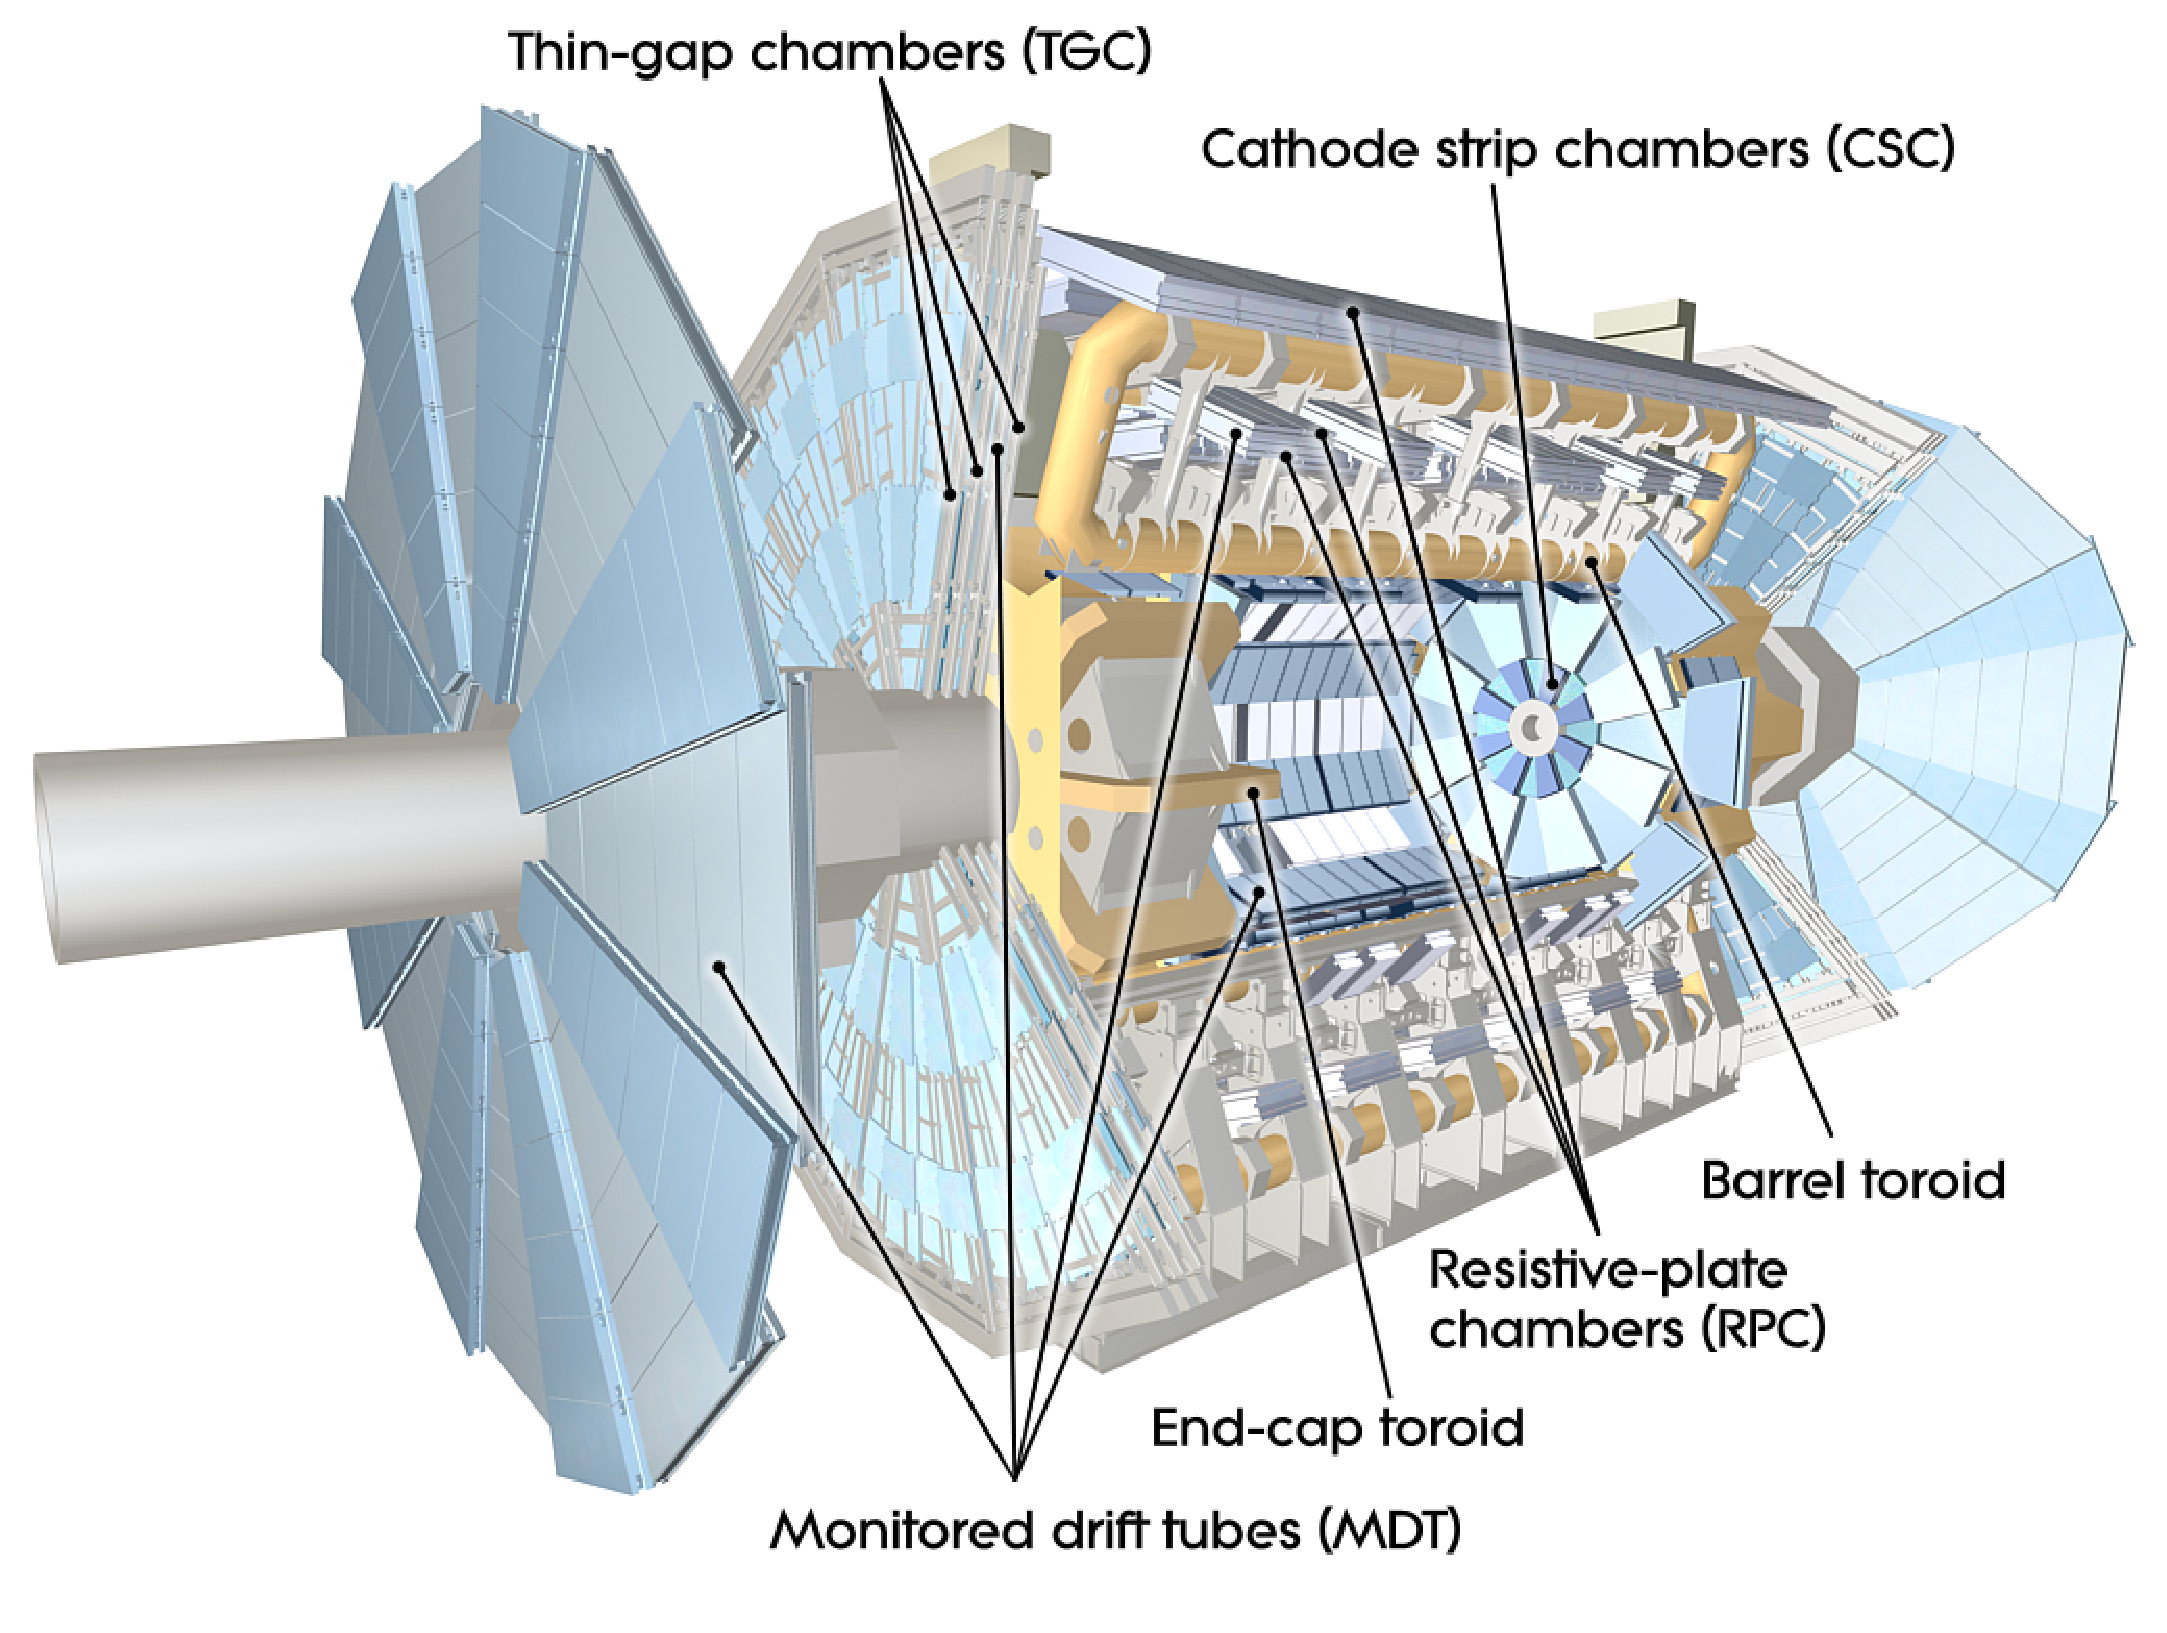
\includegraphics[scale=0.4]{images/MuonSystem_d3.eps}
			\end{center}
			\caption{ Cut-away view of the ATLAS muon system \cite{Aad:1129811}.}
			\label{fig:ATLAS_muon}
		\end{figure}

		Due to the penetrative nature of muons, all the layers of detector discussed above do not induce the showering of high energy muons. Therefore the outermost detector is another tracking detector specifically for muons. It uses the outer toroid magnet system to bend muon paths and measure muon momentum. The Muon Spectrometer is composed of 4 different technologies; Monitor Drift Tubes (MDT), Cathode Strip Chambers (CSC), Resistive Plate Chambers (RPC) and Thin Gap Chambers (TGC). Both the MDT and the CSC boast precision tracking but both have slow readout times. The RPCs and TGCs have the job of triggering muons and providing additional track measurements. The RPCs are found in the barrel region ($|\eta|~<~1.05$) while the TGC trigger in the endcap region ($1.05~<~|\eta|~<~2.4$). The MDT covers a full range in $\eta$ ($|\eta|~<~2.7$) with complementary measurements from the CSC at $2.0~<~|\eta|~<~2.7$.\\
		%(- detector alignment)
		%(- no. chambers?)




\newpage
\chapter{The Trigger \& Data Acquisition}

	The trigger system within ATLAS \cite{Aad:1129811} is designed to manage the high rate of events produced by the LHC and bring them down to a total rate that can be written to permanent storage by selecting ``interesting'' events. The related Data Acquisition (DAQ) system controls the flow of data from detector hardware through the trigger system to permanent storage at CERN and the worldwide tier 1 grid sites. 

	The trigger system is made up of three main decision levels; Level 1, Level 2 and Event Filter. Level 1 (L1) is mainly hardware based using limited detector information to locate regions of interest (RoIs) and pass them the Level 2. The Level 2 (L2) system checks the RoIs with full detector granularity and precision and the last stage the Event Filter (EF) uses analysis reconstruction techniques to further select ``interesting'' events down to the level of 400-500 Hz. Both the L2 and EF triggers compose what is called the High-Level-Trigger (HLT) together with the event building software needed by the EF. Figure \ref{fig:triggerFlow} shows the over all trigger system and how data flows through it.

	\begin{figure}[h]
        \begin{center}
            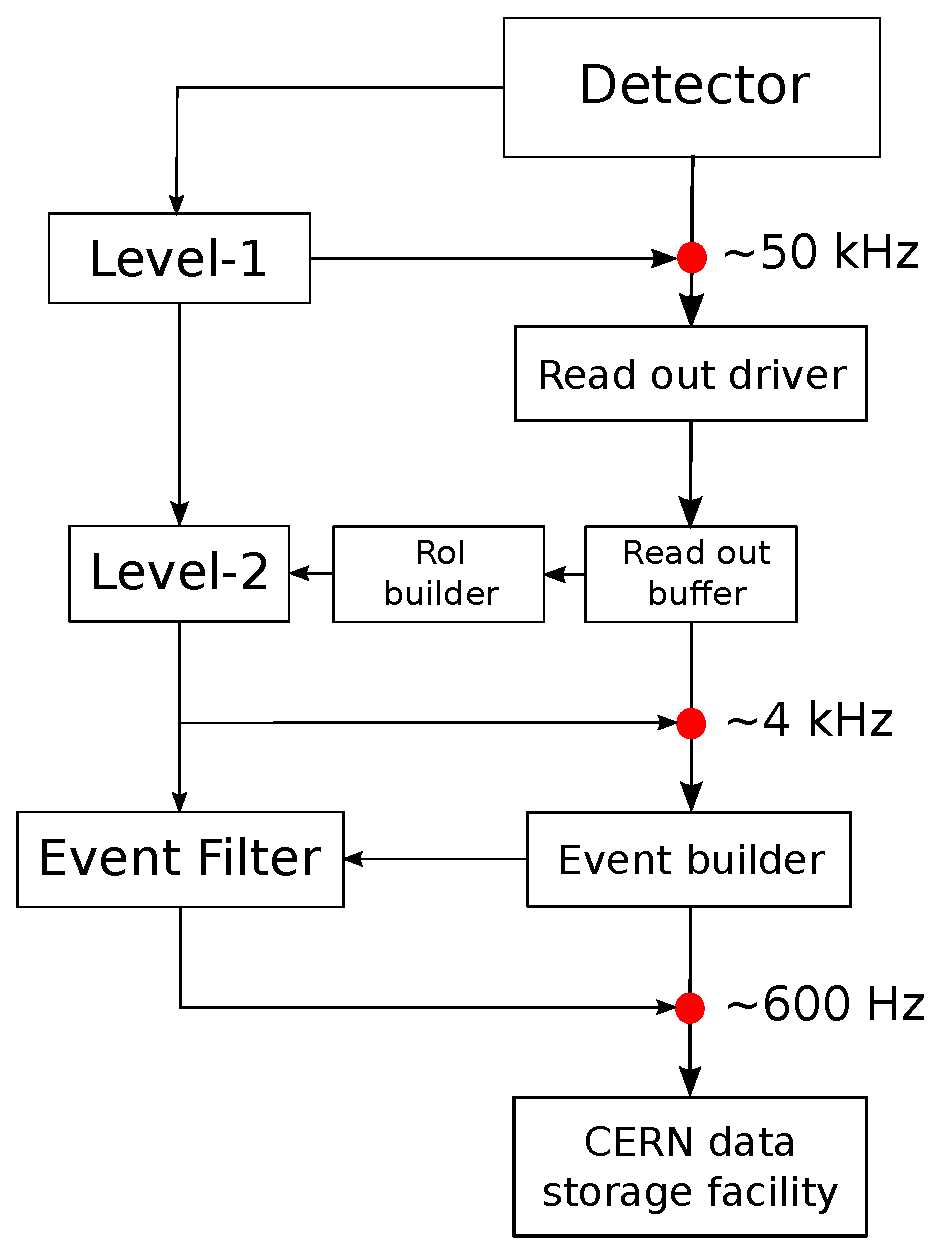
\includegraphics[width=0.7\linewidth]{images/Trigger_system.eps}
        \end{center}
        \caption{Diagram showing the different stages of the trigger and how they interact. Red points indicate points of acceptance for each trigger and numbers show the approximate number of events accepted per second at the end of the 8 TeV run in 2012.}
        \label{fig:triggerFlow}
    \end{figure}


	Following is a description of each of the sections of the trigger while focusing on the selection of electron objects that are relevant for this analysis. Following this is a discussion of how the trigger menus are formed so bandwidth can be shared between the differing physics goals as well as how ATLAS handles the continued high luminosity push of the LHC.


\section{Level-1 Trigger}

	The Level 1 (L1) trigger searches for RoI's consisting of strong signatures, i.e. high energy, muons, electron/photons or jets. The L1 trigger also searches for events with a large missing transverse energy ($E^{miss}_{T}$) or large total transverse energy ($\Sigma E_{T}$). Due to the decision speed required only some parts of the detector can be used at L1 (and at a much coarser granularity than is possible at the later stages). For muon triggering only the RPC's and TGC's can be used while for electromagnetic clusters and jets as well as large $E^{miss}_{T}$ and $\Sigma E_{T}$ the full calorimetry system can be used. The Inner Detector is not used in L1 decisions due to the time constraint. With a beam crossing interval of 50 ns, at the trigger latency is required to be less than \SI{2.5}{\us} with a target of \SI{2.0}{\us}. However half of this quota, about \SI{1.0}{\us}, is accounted for by the cable propagation of signals.

	%(- pipeline memories)
	%(- where and what these calculations are carried out on?)

	The L1Calo system uses trigger towers with a granularity reduced to roughly $0.1 \times 0.1$ in $\Delta\eta \times \Delta\phi$ in most of the detector range from both the electromagnetic and hadronic calorimeters. The ECAL produces almost 3500 of these trigger towers via summation of the analogue signals from a range of trigger cells. This trigger tower data is then sent to the Cluster Processor (CP) to identify electron/photon and tau candidates with $E_{T}$ above a required threshold and passing isolation requirements, which are labelled as RoI's.

	\begin{figure}[h]

		\begin{center}
			$\vcenter{\hbox{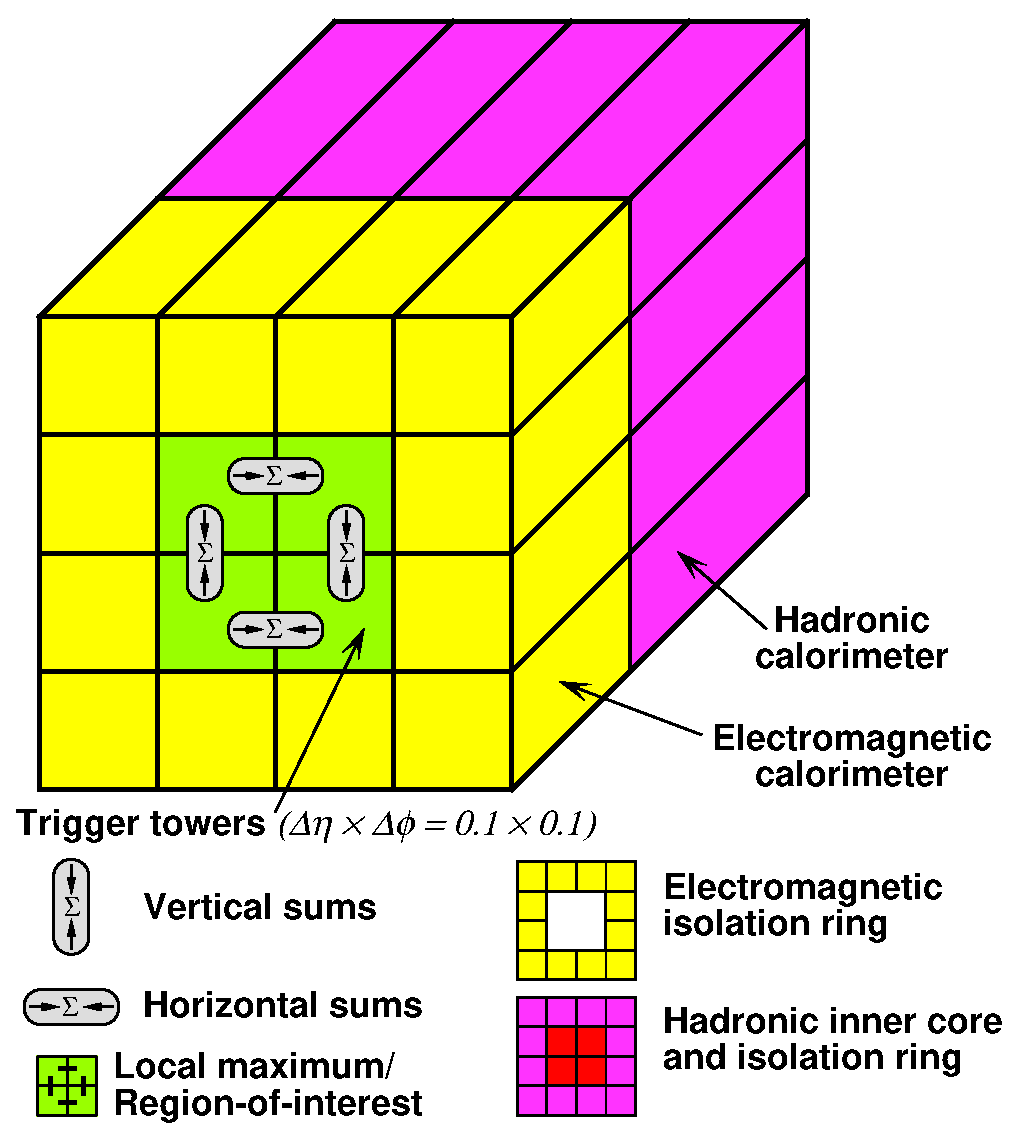
\includegraphics[width=0.4\linewidth]{images/EGammaTauAlgo.eps}}}$
			\hspace*{.5in}
			$\vcenter{\hbox{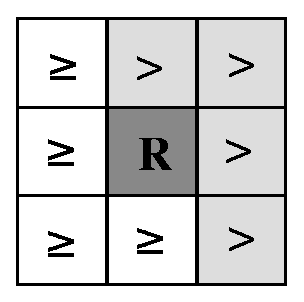
\includegraphics[width=0.4\linewidth]{images/LocalMax.eps}}}$
		\end{center}
		\caption{ Electron/photon and tau trigger algorithms (left) and E$_{T}$ local-maximum test for a cluster/RoI candidate (right). (The eta-axis runs from left to right, and the phi-axis from bottom to top. The symbol R refers to the candidate 2x2 region being tested.)}
		\label{fig:Trig_algo}
	\end{figure}


	Figure \ref{fig:Trig_algo} shows how the electron/photon trigger clustering algorithm works by identifying $2 \times 2$ clusters of trigger towers within which two adjacent towers sum to greater than the triggering threshold defined in the trigger menu (seen in section \ref{sec:trig_menu}). Also shown is how three forms of isolation can be applied at this stage: the 12-tower surrounding ring, the $2 \times 2$ hadronic core behind the RoI and the 12-tower surrounding ring in the hadronic calorimeter. Only the hadronic core isolation has so far been used in electron/photon triggers within ATLAS. 
	As all possible $2 \times 2$ clusters are observed in this way it is possible to have double counting of RoIs and so the sum of each $2 \times 2$ RoI must be greater than each of its eight nearest overlapping neighbours. Figure \ref{fig:Trig_algo} also shows how this local-maxima is tested to avoiding identical sums through use of `greater than' and `greater than or equal to' in differing $\eta$ and $\phi$ directions. So if two adjacent $2 \times 2$ clusters have the same combined energy sum the one to the top or right is chosen so as not to delay the trigger process.
	The final L1 trigger decision is made by the Central Trigger Processor (CTP) which takes information from both the CP and jet algorithm as well as the L1 muon trigger. If an accept decision is made then RoI's are sent to the RoI builder which seeds the L2 trigger system and all L1 sub-systems are read out via Readout Drive's (ROD's)(discussed in section \ref{sec:trig_DAQ}) to the DAQ system for monitoring of the L1 trigger system offline.



\section{Higher Level Trigger}

	\subsection*{Level-2 Trigger}

		The Level-2 (L2) trigger is seeded by and only makes decisions based on the RoI's supplied by the L1 trigger. However it does this with full detector information and so the first stage of this trigger is a RoI builder. The RoI builder requests detector information for all relevant detectors for the observed RoI, including at this level the Inner Detector. In the case of electrons this includes the inner tracking detector, the electromagnetic calorimeter and the hadronic calorimeter. It is at L2 that a distinction between electrons and photons can be made due to existence of an associated track in the ID to the RoI in the ECAL. The RoI builder identifies calorimeter clusters and nearby tracks in order for the L2 trigger to make its decision based on algorithms reconstructing shower shapes, track-cluster matching and $E_{T}$ thresholds with isolation. The list of these requirements are held within trigger chains each designed to accept specific physics signatures (see section \ref{sec:egammaMenu}). The general idea is simply to check if RoI's still exist under closer inspection in order to reduce the rate of events before full event building takes place in the Event Filter.


		%(-L2SV supervisor?, L2PU's processing unit)


	\subsection*{Event Filter}
		The Event Filter (EF) does not differ in approach from the L2 trigger it is purely a further test of the signals handed over from L2. At this level a full reconstruction of the event takes place and EF trigger requirements with slightly more stringent thresholds are applied to the event. This is the final decision for whether the event is going to be copied to permanent storage and so the EF reduces the final acceptance rate down to the 400 - 600 Hz required by CERN's computing systems. The requirements at the EF level are also those used in ATLAS analysis so as to treat MC and data samples the same. These requirements are discussed in section \ref{sec:egammaMenu}.
	



\section{Data Acquisition}
\label{sec:trig_DAQ}

	The Data Acquisition (DAQ) system is the set of systems that control the flow of data from detectors, through the trigger and in to permanent storage. The first stage of this process is the Readout System (ROS) a set of 145 PC's or nodes which manages the collection of all detector sub-system data and L1 trigger output from ATLAS. This system is helped by Readout Drivers (ROD's) which interface directly with detector components and Readout Links (ROL's), direct point-to-point readout connecting the ROD's with the ROS's. Table \ref{tab:DAQ_readouts} shows the number of readouts for each component of the detector and L1 system.


	\begin {table}[h!]
	\begin{center}
		\begin{tabular}{ | l | l | l | c | c | c | }% c | }
		\hline
\multicolumn{3}{|c|}{Detector Partition}											& Number of & Number of & Number of \\% & Data per L1A signal 	\\
\multicolumn{3}{|c|}{ }																& ROD’s 	& ROL’s 	& ROS’s 	\\% & (kbyte)				\\
		\hline
\multirow{11}{*}{Inner detector} 	& \multirow{3}{*}{Pixel} 	& Layer 0 			& 44 		& 44 		& 4 		\\% & \multirow{3}{*}{60}	\\
									&  							& Disks 			& 24 		& 24 		& 2 		\\% & 						\\
									&							& Layers 1–2 		& 64 		& 64 		& 6 		\\% &						\\
									\cline{2-6}
									& \multirow{4}{*}{SCT}		& End-cap A 		& 24 		& 24 		& 2 		\\% & \multirow{4}{*}{110}	\\
									& 							& End-cap C 		& 24 		& 24 		& 2 		\\% &						\\
									& 							& Barrel A 			& 22 		& 22 		& 2 		\\% & 						\\
									& 							& Barrel C 			& 22 		& 22 		& 2 		\\% &						\\
									\cline{2-6}
									& \multirow{4}{*}{TRT}		& End-cap A 		& 64 		& 64 		& 6 		\\% & \multirow{4}{*}{307}	\\
									& 							& End-cap C 		& 64 		& 64 		& 6 		\\% &						\\
									& 							& Barrel A 			& 32 		& 32 		& 3 		\\% & 						\\
									& 							& Barrel C 			& 32 		& 32 		& 3 		\\% & 						\\
		\hline
\multirow{10}{*}{Calorimetry}		& \multirow{4}{*}{Tile}		& Barrel A 			& 8 		& 16 		& 2 		\\% & \multirow{4}{*}{48}	\\
									& 							& Barrel C 			& 8 		& 16 		& 2 		\\% &						\\
									& 							& Extended barrel A & 8 		& 16 		& 2 		\\% &						\\
									&							& Extended barrel C & 8 		& 16 		& 2 		\\% &						\\
									\cline{2-6}
									& \multirow{6}{*}{LAr}		& EM barrel A 		& 56 		& 224 		& 20 		\\% & \multirow{6}{*}{576}	\\
									& 							& EM barrel C 		& 56 		& 224 		& 20 		\\% &						\\
									& 							& EM end-cap A 		& 35 		& 138 		& 12 		\\% &						\\
									& 							& EM end-cap C 		& 35  		& 138 		& 12 		\\% &						\\
									&							& HEC 				& 6 		& 24 		& 2 		\\% &						\\
									& 							& FCal 				& 4 		& 14 		& 2 		\\% &						\\
		\hline
									& \multirow{4}{*}{MDT}		& Barrel A 			& 50 		& 50 		& 4 		\\% & \multirow{4}{*}{154}	\\
									& 							& Barrel C 			& 50 		& 50 		& 4 		\\% &						\\
Muon								& 							& End-cap A 		& 52 		& 52 		& 4  		\\% &						\\
spectrometer						& 							& End-cap C 		& 52 		& 52 		& 4 		\\% &						\\
									\cline{2-6}
									& \multirow{2}{*}{CSC} 		& End-cap A 		& 8 		& 8 		& 1 		\\% & \multirow{2}{*}{10}	\\
									&							& End-cap C 		& 8 		& 8 		& 1 		\\% &						\\
		\hline
\multirow{9}{*}{L1}					& \multirow{3}{*}{Calorimeter} & CP				& 4 		& 8 		& 1  		\\% & \multirow{2}{*}{28 (can be varied)} \\
									& 							& JEP 				& 2 		& 8 		& 1 		\\% &						\\
									& 							& PP 				& 8 		& 32 		& 3 		\\% &						\\
									\cline{2-6}
									& \multirow{2}{*}{Muon RPC} & Barrel A 			& 16 		& 16 		& 2 		\\% & \multirow{2}{*}{12} 	\\
									& 							& Barrel C 			& 16 		& 16 		& 2 		\\% &						\\
									\cline{2-6}
									& \multirow{2}{*}{Muon TGC} & End-cap A 		& 12 		& 12 		& 1 		\\% & \multirow{2}{*}{6}	\\
									& 							& End-cap C 		& 12 		& 12 		& 1 		\\% & 						\\
									\cline{2-6}
									& \multicolumn{2}{c|}{MUCTPI} 					& 1 		& 1 		& 1 		\\% & 0.1					\\
									& \multicolumn{2}{c|}{CTP}						& 1 		& 1 		& 1 		\\% & 0.2					\\
		\hline
\multicolumn{3}{|r|}{Total}															& 932 		& 1574 		& 145 		\\% & 1311					\\
    	\hline
  		\end{tabular}
  	\caption{Numbers of readout drivers (ROD’s), readout links (ROL’s) and readout systems (ROS’s) per detector partition at design \cite{Aad:1129811}.}%, as well as expected data size per L1A signal for a luminosity of 1034 cm$^{-2}$ s$^{−1}$.}
  	\label{tab:DAQ_readouts}
  	\end{center}
	\end {table}


  	Each ROS PC contains Readout Buffer Module's (ROBIN's), custom PCI-X cards, each containing three Readout Buffers (ROB's), at the end of each ROL. The ROB's is where event data is stored while the L2 trigger makes its decision which comes from the set of 10 L2 Supervisor (L2SV) nodes. This decision is then made by the DataFlow Manager (DFM) on input from all the L2SV nodes and sends a command to the ROS's to either expunge data or forward it on to the event building nodes (or Sub farm Input, SFI). Once a event fully built it is sent forward to the HLT farm which makes the EF decision, then and only then is a message sent back down via the DFM for the ROS's to fully delete all data from the event. The HLT farm is the largest computing resource in the DAQ system with 1116 nodes each containing 8 CPU's. These nodes can either be configured to run as the EF or L2 Processing Units (L2PU's) for the L2SV and are reconfigured as need dictates. As the final step if an event is accepted by the EF all data is passed to the Sub Farm Output (SFO) where it is stored before transfer to CERN's central data-recording facility. In the case that this connection to CERN is offline for some reason ATLAS is able to store about 24 hours worth of data in the SFO's so no data is lost.
  	Table \ref{tab:DAQ_comp} shows the number of each DAQ component used within ATLAS all of which are found in the USA15 service cavern next to the ATLAS cavern.


	\begin {table}[h!]
	\begin{center}
  	\begin{tabular}{ | l | c | c | c | }%c | c | }
		\hline
		Component & Number of & Number of & Number of \\%& Memory (Gbyte) & Type of CPU \\
		& nodes & racks & CPU’s/node \\
		\hline 
		ROS & 145 & 16 & 1 \\%& 0.512 & 3.4 GHz Irwindale \\
		\hline
		DFM & 12 & 1 & 2 \\%& 2 & 2.6 GHz Opteron 252 \\
		L2SV & 10 & 1 & 2 \\%& 2 & 2.6 GHz Opteron 252 \\
		SFI & 48 & 3 & 2 \\%& 2 & 2.6 GHz Opteron 252 \\
		HLT & 1116 & 36 & 8 \\%& 8 & Xeon E5320 1.86 GHz \\
		SFO & 6 & 2 & 2 \\%& 4 & Xeon E5130 2.0 GHz \\
		\hline
		Monitoring & 32 & 4 & 4 \\%& 8 & Xeon E5160 3.0 GHz \\
		Operations & 20 & 4 & 2 \\%& 4 & Xeon E5130 2.0 GHz \\
    	\hline
  	\end{tabular}
  	\caption{The main data-acquisition system components deployed for initial operation: the readout system (ROS), the event-building node (SFI), the data flow manager (DFM), the L2 supervisor (L2SV), the high-level trigger (HLT) and the event filter output nodes (SFO) \cite{Aad:1129811}.}
  	\label{tab:DAQ_comp}
  	\end{center}
	\end {table}


\section{Trigger Menu and Rates}
\label{sec:trig_menu}

	In its simplest form a single trigger is an energy threshold designed to select a high percentage of particles of a selected type. ATLAS contains many of these thresholds to select many interesting physics objects which are roughly grouped in to similar signatures called streams. The trigger streams are egamma ($e/\gamma$) triggers to select electrons and photons, JetTauEtMiss triggers to select hadronic decays, tau decays and large missing transverse energy, Muon triggers to select muons, MinBias trigger to check no biases exist in other triggers and cosmics triggers to selected signals of cosmic radiation. Each stream has an allocated bandwidth for readout from the trigger so all triggers need to be optimised so total acceptance rates are within requirements. Each trigger at the HLT level is designed to select a specific type of signal while those a L1 are more general and seed many HLT triggers. A full run through all three stages of the trigger is called a trigger chain. Each trigger in a trigger chain needs to not only be optimised to satisfy rate constraints but also for a high efficiency in the targeted region. In terms of energy threshold this means an increasing threshold through the trigger chain so that each level is selecting within the range close to $100\%$ efficient from the previous requirement when taking in to account the different accuracy of energy measurement provided by each level. This section focuses on the egamma trigger stream as all objects in this analysis where selected using it.

	%Figure \ref{} shows the acceptance rates of each level of the trigger for two example LHC runs one in 2011 and one in 2012. It can be seen that the acceptance rate slowly drops throughout the run because of the decease in instantaneous luminosity 


	%-jets stream used in the fake rates method?


	\subsection{\texorpdfstring{The ``$e/\gamma$'' Trigger Menu}{The ``e/gamma'' Trigger Menu}} 
		\label{sec:egammaMenu}

		The $e/\gamma$ trigger menu that is used in this analysis refers to the trigger chains designed to select electron and photon objects, detailing requirements for all three stages of the trigger. ATLAS uses its own terminology to name these triggers with the name giving a description of the requirements used. At L1 electron and photon objects are selected with triggers bearing the name EMXY where; `EM' refers to EM calorimeter, X is the value of the energy threshold required of RoIs in GeV and Y refers to any other specification. Other specifications can be `V', a threshold varying with the geometric location in the detector ($\eta$) around the given value to optimise selection, or `H', indicating hadronic isolation applied in the RoI, both of which are discussed in section \ref{sec:TrigRates}. An example of a L1 trigger is then L1\_EM18VH which is a trigger with an energy threshold of 18 GeV which is varied slightly throughout the detector and has a hadronic isolation requirement. L2 and EF use the same terminology but are prepended with either L2 or EF. They take the form such as e22vh\_medium where `e' represents an electron (g is used for photons), `vh' represents the same as above and `medium' refers to an associated set of shower shape and tracking requirements. As well as `medium', `loose' and `tight' are also defined giving looser and tighter requirements respectively. These shower shape and tracking requirements are discussed in section \ref{sec:ReconElec}. Section \ref{sec:TrigRates} discusses the development of the L1\_EM16VH trigger which feeds in to L2\_e20vh\_medium and then in to EF\_e22vh\_medium. 

		The 8 TeV analysis discussed in this thesis uses a photon trigger even though searching for electrons. This is because photon and electron triggers are identical save for tracking requirements for electrons and for the 2012 run the lowest energy triggers without hadronic isolation that were applicable for high energy dielectron decays was a diphoton trigger chain. It is important that the trigger used did not have hadronic isolation due to the very high energy nature of the electrons in this analysis which have a higher chance of leaking through in to the hadronic calorimeter. The trigger used for the 8 TeV analysis is EF\_g35\_loose\_g25\_loose which selects two photon objects with thresholds of 35 GeV and 25 GeV while both requiring `loose' shower shape requirements. This trigger is seeded by L2\_g30\_loose\_g20\_loose which itself is seeded by L1\_2EM12\_EM16V. EF\_g35\_loose\_g25\_loose reaches close to 100\% efficency of selecting two electron just above an electron energy of 40 GeV and maintains this to very high energy. The 7 TeV analysis used the trigger EF\_g20\_loose.

		% efficency plot

	\subsection{Trigger Rates in High Luminosity Regime}
		\label{sec:TrigRates}

		Due to the bandwidth limitations each level of the trigger is restricted to a certain output rate. During 2011 the L1 output rate was kept below 60 kHz, L2 below 5 kHz and the EF output rate at $\sim$ 400 Hz averaged over the LHC fills. The bandwidth allocated to the $e/\gamma$ triggers was approximately 30\% of the total EF output rate however throughout 2011 the luminosity continued to increase putting pressure on the trigger's ability to control the output rate. Several methods were employed to reduce the trigger rate and in the $e/\gamma$ trigger a variable threshold and hadronic core isolation were investigated to reduce the rate of the Level-1 trigger. In order to keep within timing constraints only a low resolution of 0.4 $\eta$ is available at L1. Threshold requirements were therefore investigated varying every 0.4 $\eta$. The effect of a hadronic core isolation was also investigated on the selection of electrons which defines a region in the hadronic calorimeter behind the $e/\gamma$ candidate in which a minimum amount of energy is required to be deposited in order to distinguish between jets and $e/\gamma$ objects. 


		A study in to introducing these new requirements \cite{ATLAS-CONF-2012-048} at L1 was carried out using data from the trigger stream with a ``tag \& probe''\footnote{A method of identifying a good electron candidate as a tag and then associating it with another probe electron where the combined dilepton invariant mass lies within the Z peak. With this probe electron you can then measure the efficiency of a set of selections.} study to calculate the efficiency of an array of new L1 requirements. Objects selected with ``tag \& probe'' were organised in to bins of 0.4 in $\eta$ and threshold of 16, 17, 18 and 19 GeV were applied as a L1 trigger. Within each 0.4 $\eta$ bin acceptance efficiency versus reconstructed transverse energy was studied. The highest threshold for which greater than 99\% efficiency was reached for a transverse energy of 22 GeV (threshold at EF) was then selected as the threshold in that region. The results of this optimisation can be seen in table \ref{tab:L1_thresh} where the threshold for each eta region is given. 

		\begin {table}[h!]
		\begin{center}
	  	\begin{tabular}{  l | c  }%c | c | }
			\hline
			$|\eta|$ region & Level-1 threshold [GeV] \\
			\hline
			$<$ 0.8 	& 18 \\
			0.8 - 1.2 	& 17 \\
			1.2 - 1.6 	& 16 \\
			1.6 - 2.0 	& 17 \\
			2.0 - 2.4 	& 18 \\
			$>$ 2.4 	& 16 \\
	    	\hline
	  	\end{tabular}
	  	\caption{Optimised L1 thresholds for the L1 EM16 trigger.}
	  	\label{tab:L1_thresh}
	  	\end{center}
		\end {table}


		Hadronic core isolations was investigated for isolation less than 1, 2 and 3 GeV. A hadronic core isolation of less than 1 GeV was chosen as this was seen to have a less that 1\% effect on acceptance. Both of these requirements then went in to the specification of the L1\_EM16VH trigger.


		Figure \ref{fig:L1} shows the performance of the trigger after these changes had been made. It can be seen that a minimal impact of these new requirements is felt in efficiency for both $\eta$ and number of primary vertices. Most importantly the ``turn on'' curve for efficiency as a function of E$_{T}$ shows the point at which 100\% efficiency is reached is not that much higher than EM16. This then introduced the new lowest threshold electron trigger chain used in ATLAS. The effect of this introduction can be seen during the middle of the year in figure \ref{fig:EF_rate} where a significant decrease in the event filter acceptance rate is seen with the introduction of this and several other trigger strategies. 


		\begin{figure}[h!]
			\centering
				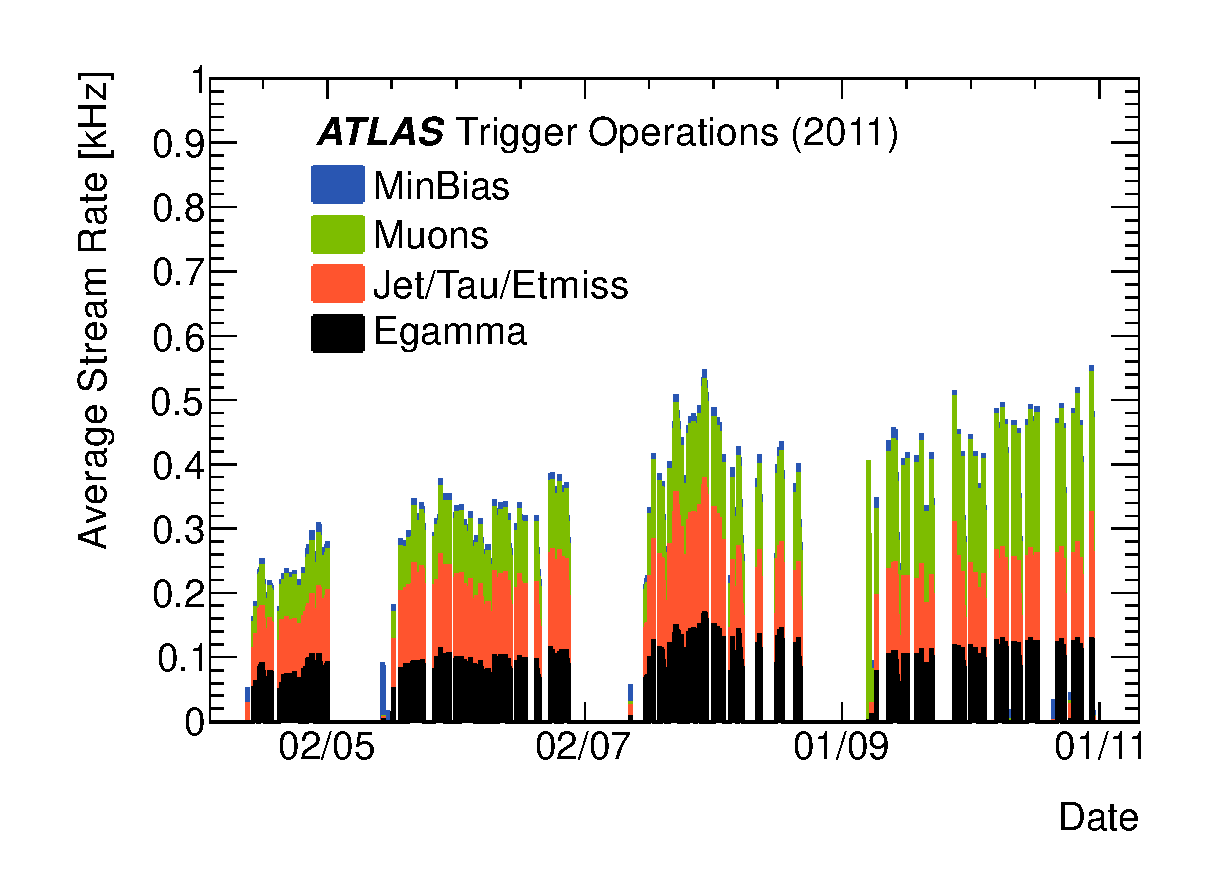
\includegraphics[width=0.75\linewidth]{images/2011_streams_quarter_day.eps}
			\caption{Event Filter stream recording rates from 2011. \cite{Trigger_op_2011}}
			\label{fig:EF_rate}
		\end{figure}


		For the 2012 run this trigger went through a revision raising the thresholds of each trigger in the chain to accommodate higher luminosity at 8 TeV, this chain is discussed in section \ref{sec:egammaMenu}. This study was completed by the author as a part of the ATLAS service task and became part of a ATLAS conference note \cite{ATLAS-CONF-2012-048}.


		\begin{figure}[h]
			\centering
				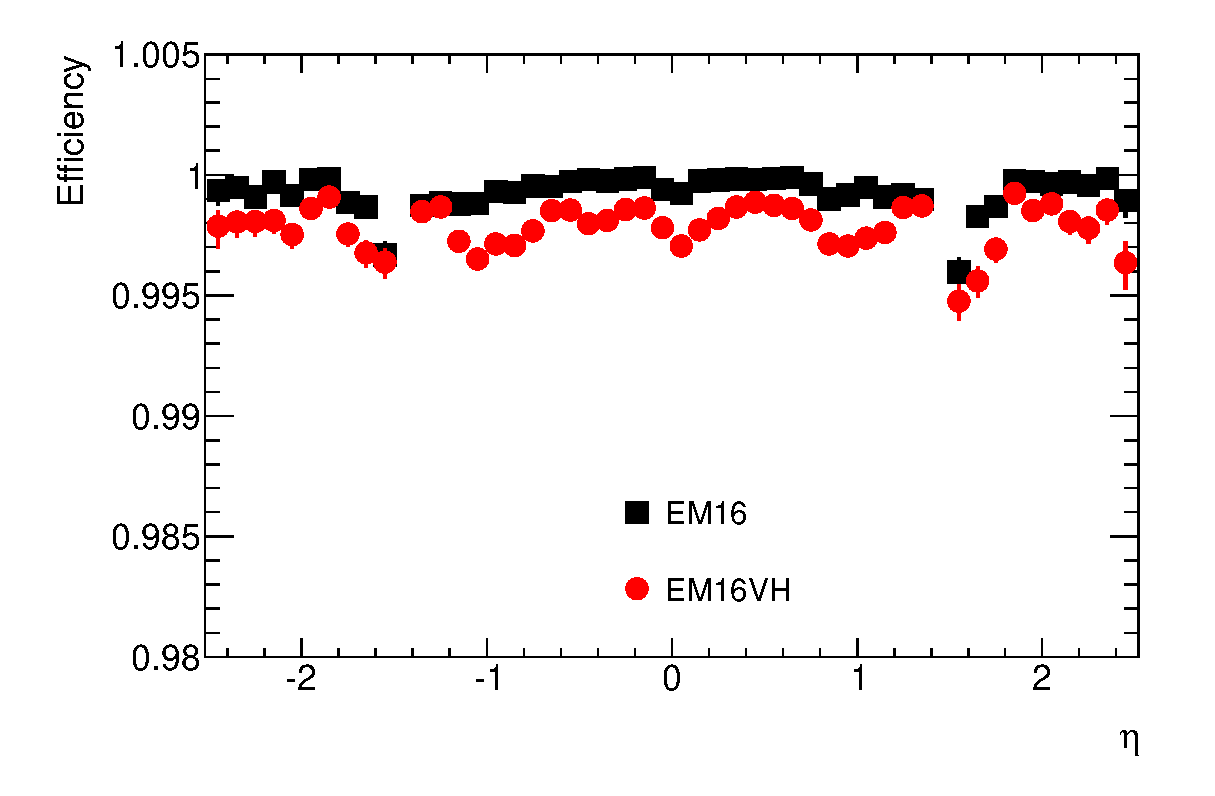
\includegraphics[width=0.78\linewidth]{images/L1_EM16VH_TandP_eff_vs_eta.eps}
				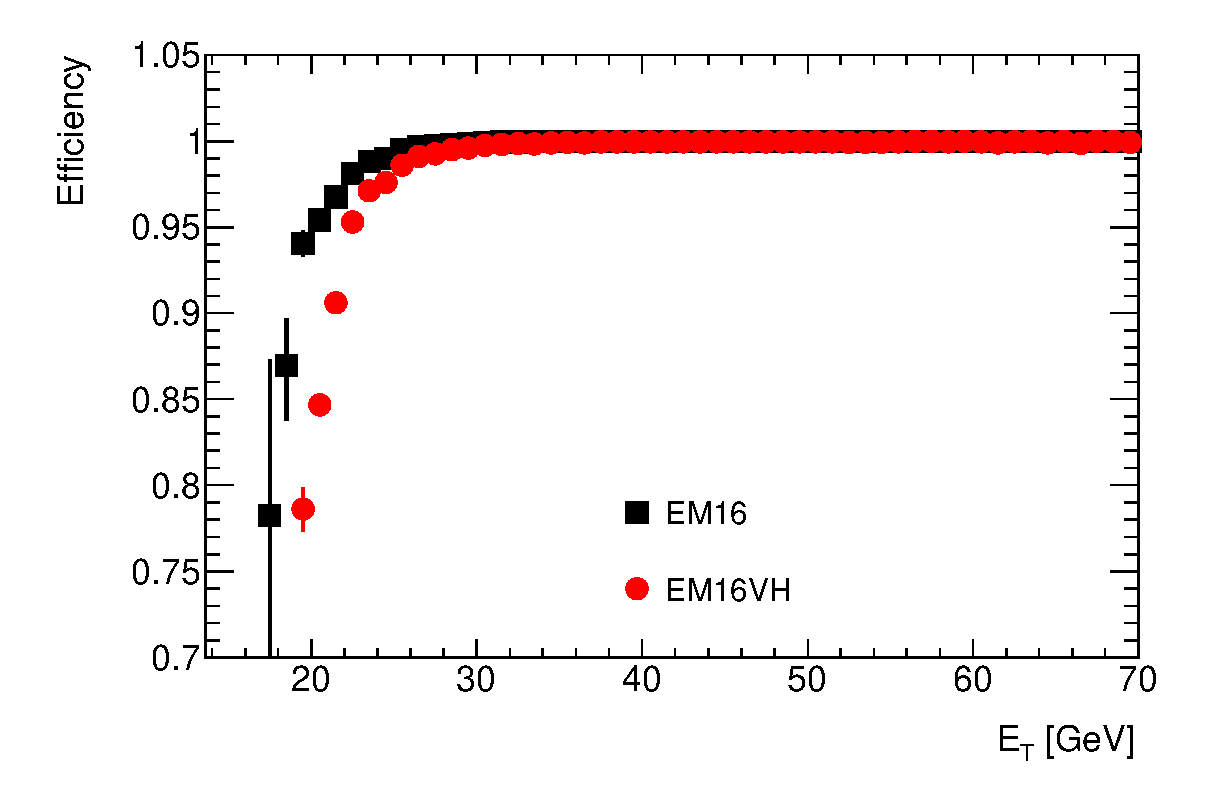
\includegraphics[width=0.78\linewidth]{images/L1_EM16VH_TandP_eff_vs_Et.eps}
				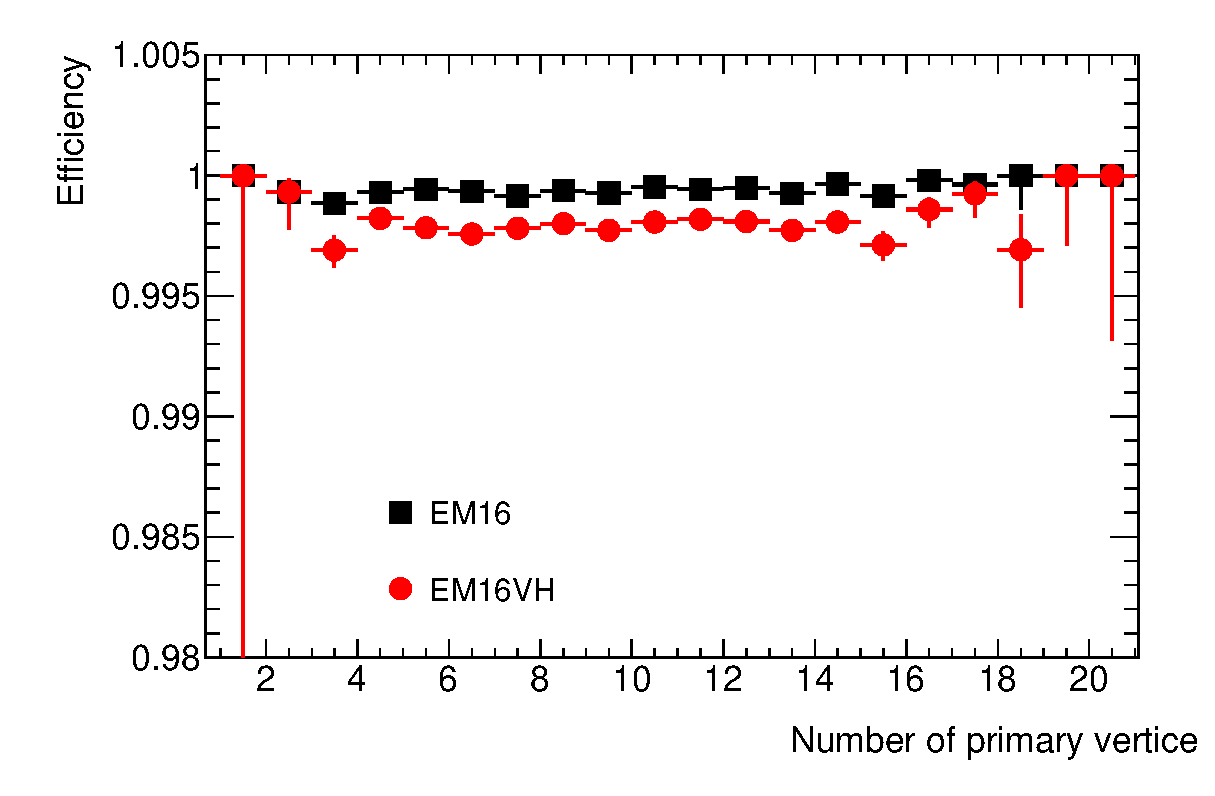
\includegraphics[width=0.78\linewidth]{images/L1_EM16VH_TandP_eff_vs_pvx.eps}
			\caption{Performance of the first level of the ATLAS $e/\gamma$ trigger before (EM16) and after (EM16VH) variable thresholds and hadronic core isolation are applied. Efficiency verse $\eta$ (top), E$_{T}$ (middle) and number of primary vertices (bottom).}
			\label{fig:L1}
		\end{figure}


		%expand...

\newpage
\chapter{Event Reconstruction}

Reconstruction is the process and algorithms that attempt to reform information about collision events and their decay products from detector signals. This process is done at several points in the ATLAS analysis procedure. First partial reconstruction of RoI's is done at the Level-2 trigger while a mostly full detector reconstruction is done at the EF. After the data has been permanently stored full reconstruction of all possible signatures in each event as well as whole event variables can be completed if it failed to finish live during the trigger decision.

The other main source of reconstruction is done in a process called reprocessing. After data has been stored updates to sub-detector calibrations and optimisations can take place and so reconstruction of entire data sets takes place to update variables to more accurate measurements. 

The Data format used in this analysis is an internal ATLAS format called a D3PD. This format is a type of ROOT \cite{} ntuple, or sequence of ordered lists, which stores ATLAS event data. The data used has past through ATLAS software reconstruction while the Monte-Carlo (MC) background estimate samples have gone through GEANT \cite{} detector simulation as well as ATLAS reconstruction. This means analysis of these D3PD's with root requires only minor corrections.


Some of the many variables reconstructed are event specific and one of the more important of this is the number of interactions per bunch crossing. As more than one proton collision takes place with each bunch collision a lot of physics background can appear in an event. This makes the search harder but it is also needs to be predicted properly by background estimates. The problem is referred to as pile-up and corrections needed to accommodate it are discussed in section \ref{sec:correc}. Figure \ref{fig:pu} shows the distribution of number of interactions per bunch crossing seen in the 7 TeV and 8 TeV ATLAS data sets.

\begin{figure}[h!]
	\centering
		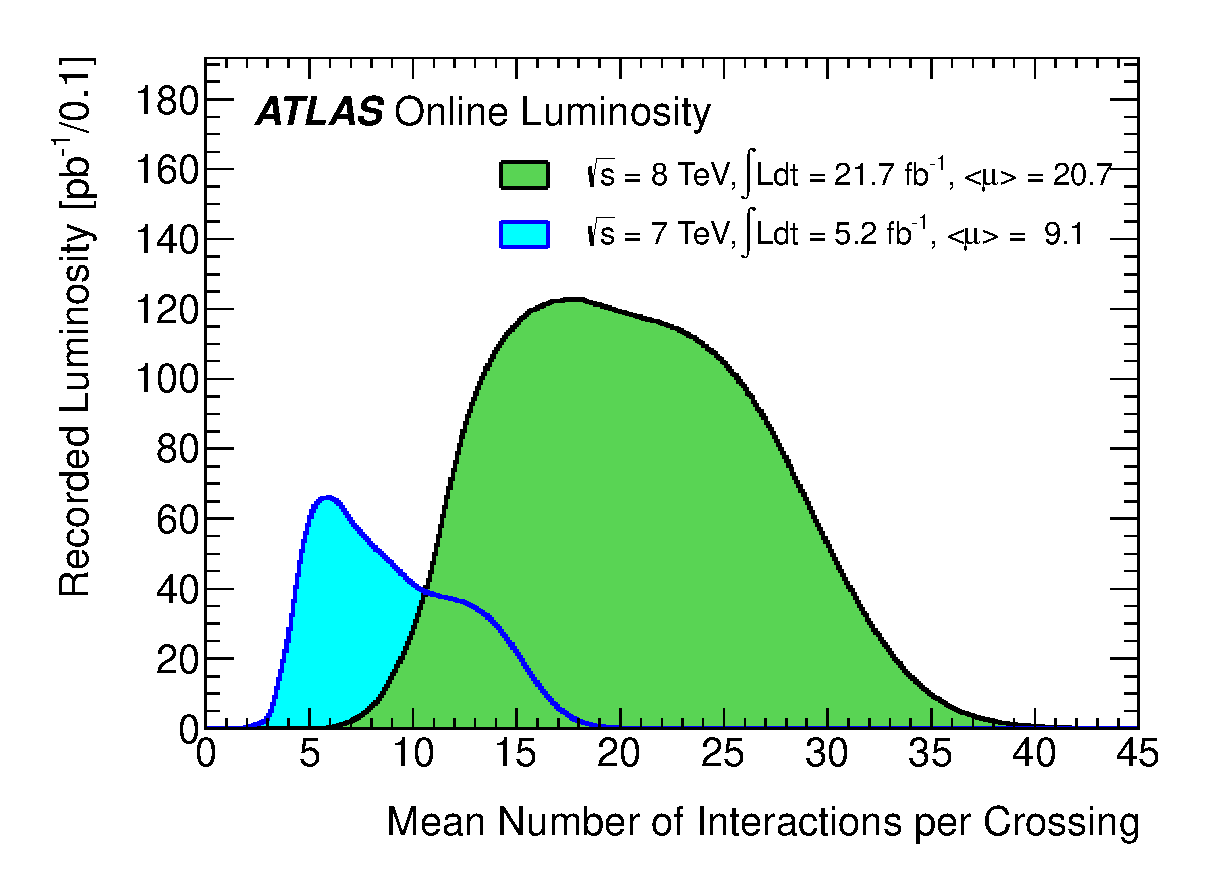
\includegraphics[width=0.8\linewidth]{images/mu_2011_2012-dec.eps}
	\caption{Luminosity-weighted distribution of the mean number of interactions per crossing for the 2011 and 2012 data. \cite{mu_2011_2012_dec,Aad:2011dr}}
	\label{fig:pu}
\end{figure}


Below will mainly be a discussion of the reconstruction of electron (and related photon) objects as these are the decay products searched for in this analysis.



\section{Electron Reconstruction and Identification}
\label{sec:ReconElec}

	During reconstruction each EM calorimeter energy signature with an associated track in the inner detector get listed as an electron object. These objects get selected via a clustering algorithm in the EM calorimeter which defines the energy and is then matched to a track. These objects then have a list of associated variables derived from detector readouts on which an analysis selection for `good' electrons can be made. These variables range from simple values of position and energy to more complex derived values such as isolation. A few variables will be listed below relevant to this analysis and how they are derived.

	\begin{itemize}
	\item $\eta$ \& $\phi$, a particle trajectory or position in detector. These are the main variables for measuring the direction the particle went in the detector and for electrons can be measured in two ways. Either via cluster location in the EM calorimeter or measurement in the inner detector.
	\item $p_{T}$ or transverse momentum. $p_{T}$ is the main measure of energy used for particles where $p_{T}~=~|p|\cosh{\eta}$. Here $\eta$ comes from either the inner detector or calorimeter cluster hit location and the choice is dependent on a how many hits the track made travelling though the inner detector and therefore how accurate the measurement is.
	\item $E_{T}$cone20. This is a cluster isolation variable measuring the sum of energy found around the region of interest minus the electron cluster for $R < 0.20$ where $R = \sqrt{\eta^{2} + \phi^{2}}$. $E_{T}$cone20 is used to check cone isolation in order to eliminate jet like signatures from the analysis which often create large showers in the calorimeters.
	\item Electron Charge. This is simple matter of measuring the direction the electron curves in the inner detector. However as discussed in chapter 5 this can be hard for very high energy electrons.
	\item loose, medium, tight. This is a definition given to a set of selections defining how certain it is the object is an electron. The selections and variables associated with this are discussed below.
	\end{itemize}

	Loose, medium and tight define an increasing series of selections for identifying good electron signatures in the detector. The selections vary between shower shape variables to track quality and track cluster matching. Some of the important associated variables are discussed in table \ref{tab:Rec_lmt} with the full selections found in appendix \ref{} as the full selections are two dimensional arrays of threshold for most selections. Also to note there are two different definitions of medium referred to as medium and medium++. The latter is a re-optimisation of the selection and slightly stricter than the original medium. medium++ is used in this analysis and found in appendix \ref{}.

	\begin {table}[h!]
	\begin{center}
  	\begin{tabular}{llc}
		\hline
		\multicolumn{3}{l}{{\bf Loose selection}} 																					\\ 
		%\hline
		Type 				& Description																	& Name 					\\
		\hline
\rule{0pt}{3ex}Acceptance 			& $|\eta|~<~2.47$ 														& $\eta$				\\
\rule{0pt}{4ex}Hadronic leakage	& Ratio of $E_{T}$ in the first layer of the hadronic calorimeter to $E_{T}$ of	& \multirow{2}{*}{$R_{had1}$}			\\
							& the EM cluster (used over the range $|\eta|~<~0.8$ and $|\eta|~>~1.37$)		&						\\
							\rule{0pt}{3ex} 
							& Ratio of $E_{T}$ in the hadronic calorimeter to $E_{T}$ of the EM cluster 	& \multirow{2}{*}{$R_{had}$}			\\
							& (used over the range $|\eta|~<~0.8$ and $|\eta|~>~1.37$)						&						\\
\rule{0pt}{4ex}Middle layer of  	& Ratio of the energy in $3\times7$ cells over the energy in $7\times7$ cells centred  	& \multirow{2}{*}{$R_{\eta}$}	\\
		EM calorimeter		& at the electron cluster position												&						\\
							\rule{0pt}{3ex} 
							& Lateral shower width, $\sqrt{(\sum{E_{i} \eta_{i}^{2}})/(\sum{E_{i}}) - ((\sum{E_{i} \eta_{i}})/(\sum{E_{i}}))^{2}}$, where  	& \multirow{3}{*}{$\omega_{\eta2}$}		\\
							& $E_{i}$ is the energy and $\eta_{i}$ is the pseudorapidity of cell $i$ and the sum is 	& 			\\
							& calculated  within a window of 3 $\times$ 5 cells								&						\\
		\hline
		\hline
		\multicolumn{3}{l}{{\bf medium \& medium++ selection} (includes loose)}																	\\
		%\hline
		Type 				& Description																	& Name 		 			\\
		\hline
\rule{0pt}{3ex}Strip layer of EM 	& Shower width, $\sqrt{(\sum{E_{i}(i - i_{max})^{2}})(\sum{E_{i}})}$, where $i$ runs over all strips in & \multirow{3}{*}{$\omega_{stot}$}	\\
		calorimeter 		& a window of $\Delta\eta~\times~\Delta\phi~\approx~0.0625~\times~0.2$, corresponding typically to  	&			\\
							& 20 strips in $\eta$, and $i_{max}$ is the index of the highest-energy strip 	& 						\\
							\rule{0pt}{3ex}
							& Ratio of the energy difference between the largest and second largest  		& \multirow{2}{*}{$E_{ratio}$}			\\
							& energy deposits in the cluster over the sum of these energies					&						\\
\rule{0pt}{4ex}Track quality	& Number of hits in the pixel detector $(\geq1)$							& $n_{pixel}$			\\
							& Number of total hits in the pixel and SCT detectors $(\geq7)$					& $n_{Si}$				\\
							& Transverse impact parameter $(|d_{0}|~<~5~\text{mm})$							& $d_{0}$				\\
\rule{0pt}{4ex}Track-cluster		& $\Delta\eta$ between the cluster position in the strip layer and the extrapolated 	& \multirow{2}{*}{$\Delta\eta$} 	\\
		matching			& track $(|\Delta\eta|~<~0.01)$													& 						\\
		\hline				
		\hline
		\multicolumn{3}{l}{{\bf Tight selection} (includes medium)}																	\\
		%\hline
		Type 				& Description 																	& Name 					\\
		\hline
\rule{0pt}{3ex}Track-cluster		& $\Delta\phi$ between the cluster position in the middle layer and the extrapolated 	& \multirow{2}{*}{$\Delta\phi$}	\\
		matching			& track $(|\Delta\phi|~<~0.02)$													& 						\\
							& Ratio of the cluster energy to the track momentum								& $E/p$					\\
							& Tighter $\Delta\eta$ requirement $(|\Delta\eta|~<~0.005)$						& $\Delta\eta$ 			\\
\rule{0pt}{4ex}Track quality		& Tighter transverse impact parameter requirement $(|d_{0}|~<~1~\text{mm})$		& $d_{0}$				\\
		TRT 				& Total number of hits in the TRT 												& $n_{TRT}$				\\
							& Ratio of the number of high-threshold hits to the total number of hits in 	& \multirow{2}{*}{$f_{HT}$}				\\
							& the TRT 																		& 						\\
\rule{0pt}{4ex}Conversions 	& Number of hits in the b-layer $(\leq1)$ 										& $n_{BL}$				\\
							& Veto electron candidates matched to reconstructed photon conversions 		 	& 						\\
		\hline
  		\end{tabular}
  	\caption{Table showing the variables associated with definitions of loose, medium and tight \cite{Aad:2011mk}. Full thresholds found in appendix \ref{}}
  	\label{tab:Rec_lmt}
  	\end{center}
	\end {table}













\newpage
\chapter{Event Selection}

The main event selection for this analysis is based on a standard cut-flow selection used within ATLAS to select high energy di-electron events. Following will be the basic outline of each requirement an event must satisfy followed by a discussion of optimisations done to some cuts for this analysis. Finally a discussion of corrections is included; spanning minor variable corrections to data obtained by performance groups after reconstruction and more substantial corrections to MC samples to correctly estimate run conditions.
The following analysis selection is applied equally to the data and MC background samples unless where noted. 


\section{Analysis Selection}

The following selection is made to all data and MC events for this analysis. Before selection several data flags are checked to insure full operation of the detector at time of data taking. \\

{\bf Event Selection}
\begin{itemize}
\item Event is required have passed the chosen unprescaled electron trigger (EF\_g35\_loose \_g25\_loose).
\item Each event is required to contain at least one reconstructed primary vertex with at least 2 traceable charged tracks.
\end{itemize}


{\bf Electron Selection}
\begin{itemize}
\item Electron $|\eta| < 2.47$ and not lie within the detector crack region $1.37 \leq |\eta| \leq 1.52$ due to a decreased energy resolution.
\item Each electron is required to have a transverse momentum ($p_{T}$) greater than 30 GeV with the highest $p_{T}$ electron lying above 40 GeV.
\item Electrons are required to pass identification criteria on the transverse shower shape, the longitudinal leakage into the hadronic calorimeter, and the association to an inner detector track, defined together as a medium++ electron identification (see section \ref{sec:ReconElec}).
\end{itemize}


{\bf Dielectron Selection}
\begin{itemize}
\item Selection of two highest $p_{T}$ electrons left in event.
\item Lead isolation (a cone around the candidate in the calorimeter is required to have  $< 0.007~\times~E_{T}~+~5.0~GeV$ deposited in it) of the highest $p_{T}$ electron in the event is used to suppress jet background. 
\item Sub-leading isolation (a cone around the candidate in the calorimeter is required to have  $< 0.0022~\times~E_{T}~+~6.0~GeV$ deposited in it) of the second highest $p_{T}$ electron in the event is used to suppress more jet background. 
\item Dielectron invariant mass (m$_{ee}$) is required to be greater than or equal 80 GeV.
\item Opposite sign requirement. Require both electrons to have opposite charge.
\end{itemize}




\section{Isolation Requirement}
   \label{sec:iso}

When optimising for the 8 TeV analysis a re-investigation of the isolation requirement was needed, updating the selection from its previous iteration in the di-electron analysis on $7~$TeV ATLAS data. The previous threshold was a flat, less than $7~$GeV, cut on the calorimeter cluster isolation ($E_{T}$cone20) of the highest E$_{T}$ electron in the selected pair. The first investigation was to see how this cut performed in the selection of MC signal at 8 TeV centre of mass energy. Due to the better statistics found in the $DY{\rightarrow}ee$ MC sample and this being an irreducible background and therefore indistinguishable from the signal this was used in the following investigation.

This flat cut of 7 GeV causes an increasing efficiency loss at high energy and was deemed unsuitably high for this iteration of the analysis due to the higher reach in energy expected from the higher centre of mass collision energy. The introduction of an isolation requirement on the second highest electron was also proposed which did not exist in the 7 TeV analysis.

The possibility was an isolation requirement varying with energy. The main source of background the isolation cut is imposed to reduce is jets that fake an electron signal in the detector. Jet backgrounds are estimated via a reverse ID method on data seen in section \ref{sec:FFmethod} with low statistics at high energy. For this reason it is hard to optimise the isolation requirement against rejection of this background at high energy. Therefore it was chosen to optimise the new selection against the acceptance of signal. This study was undertaken by the author to optimise the isolation requirement. 

Figure \ref{fig:C5_leadIso_vs_leadpT} shows the distribution of DY MC events in $E_{T}$ and cluster isolation. It can be seen that electrons become less isolated under this definition of isolation as energy of the electron increases. This is to be expected as higher energy electrons produce larger showers and spread out over many EM calorimeter cells. 

   \begin{figure}[h!]
      \begin{center}
      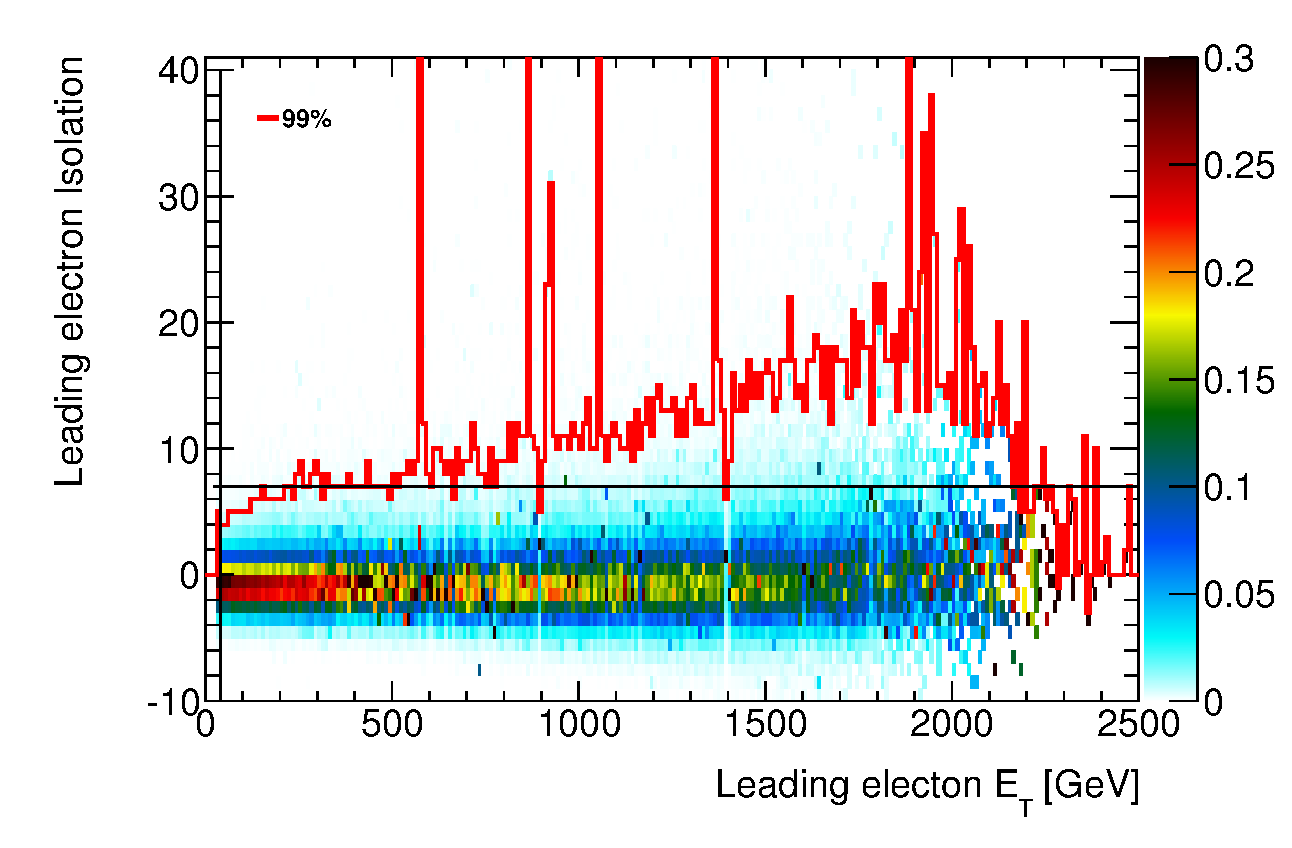
\includegraphics[scale=0.7]{images/C5_leadIso_vs_leadpT.eps}
      \end{center}
   \caption{Distribution of DY MC in $E_{T}$ and cluster isolation for the highest energy electron. Colour density shows the fraction of electons from that $E_{T}$ column found in the cell. The red line shows the 99\% acceptance point of electrons in the $E_{T}$ column. While the black vertical and horizontal lines show the $p_{T}$ and old isolation cut respectively.}
   \label{fig:C5_leadIso_vs_leadpT}
   \end{figure}


In order to define a requirement varying in E$_{T}$, the 99\% acceptance point for each E$_{T}$ column was calculated and a first order polynomial fit to these points was done by eye. The 99\% acceptance points can be seen in figure \ref{fig:C5_leadIso_vs_leadpT} and this as well a the fit can be seen in figure \ref{fig:C5_leadIso_vs_leadpT_proposal}. The same thing was calculated for the second highest E$_{T}$ electron and can be seen in figure \ref{fig:C5_subIso_vs_subpT_proposal}.


   \begin{figure}[h!]
      \begin{center}
      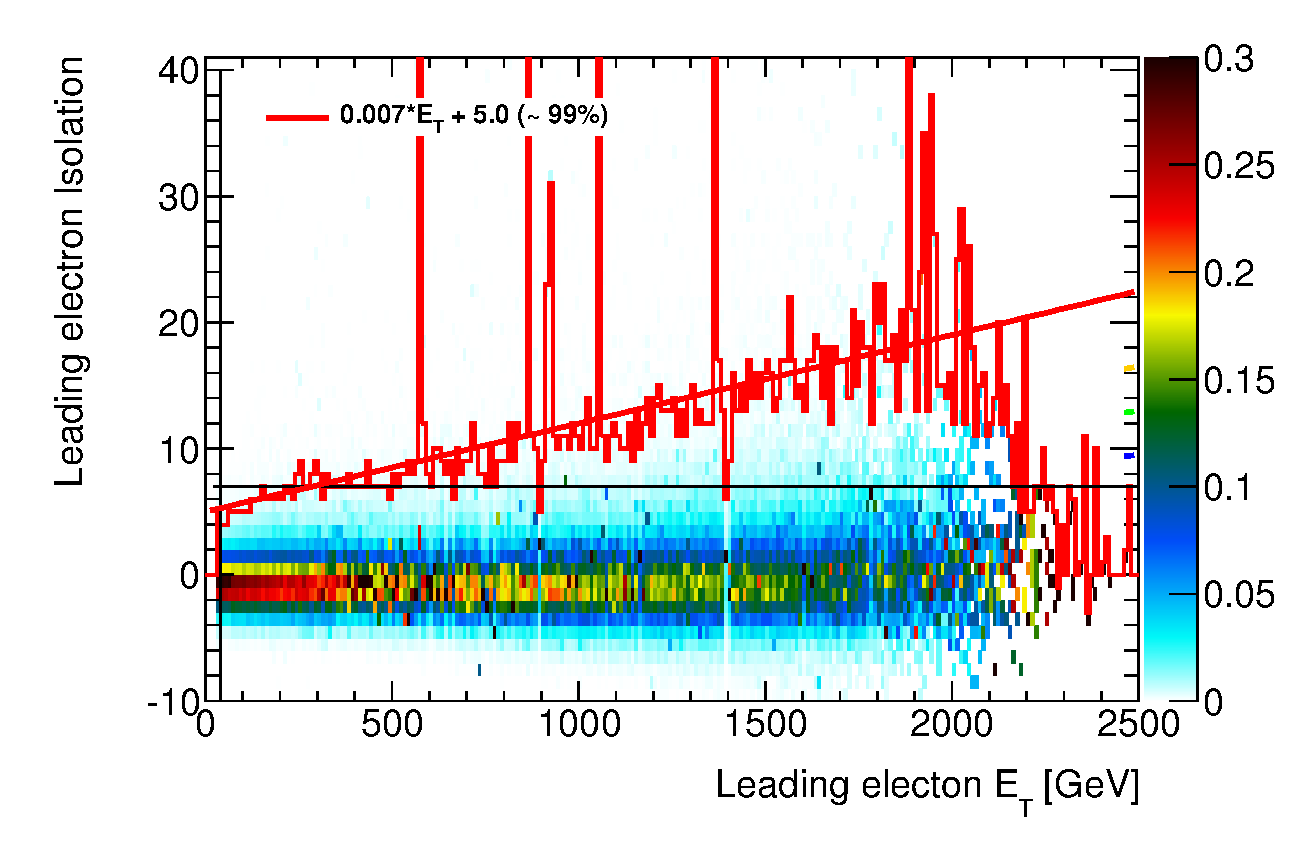
\includegraphics[scale=0.7]{images/C5_leadIso_vs_leadpT_proposal.eps}
      \end{center}
   \caption{Similar plot to figure \ref{fig:C5_leadIso_vs_leadpT} but with a fit to 99\% efficiency suggested as a possible isolation requirement.}
   \label{fig:C5_leadIso_vs_leadpT_proposal}
   \end{figure}


   \begin{figure}[h!]
      \begin{center}
      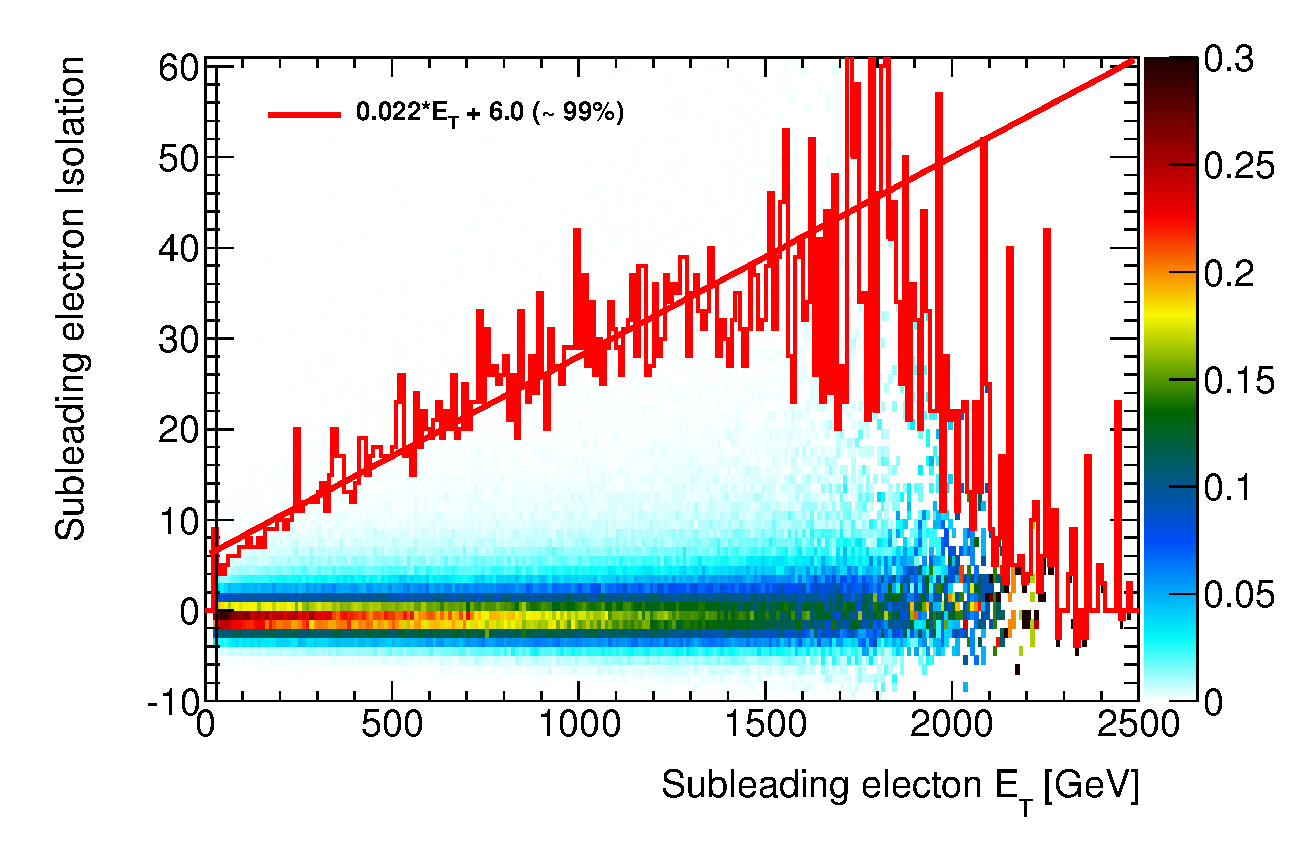
\includegraphics[scale=0.7]{images/C5_subIso_vs_subpT_proposal.eps}
      \end{center}
   \caption{Similar plot to figure \ref{fig:C5_leadIso_vs_leadpT_proposal} but for second highest energy electrons after the 99\% isolation efficiency selection is applied to the highest energy electron.}
   \label{fig:C5_subIso_vs_subpT_proposal}
   \end{figure}



The two first order polynomials shown here correspond to isolation requirements of;
   \begin{center}
   $Lead~Isolation < 0.007\times~E_{T}~+~5.0~GeV$\\
   $Subleading~Isolation < 0.022\times~E_{T}~+~6.0~GeV$\\
   \end{center}
for the highest and second highest energy electrons respectively. 

An analysis of the efficiency of these cuts on signal can be seen in figures \ref{fig:C5_lead_iso_efficiency} and \ref{fig:C5_sub_iso_efficiency} where it can be seen they maintain a flat behaviour as $E_{T}$ increases.


   \begin{figure}[h!]
      \begin{center}
      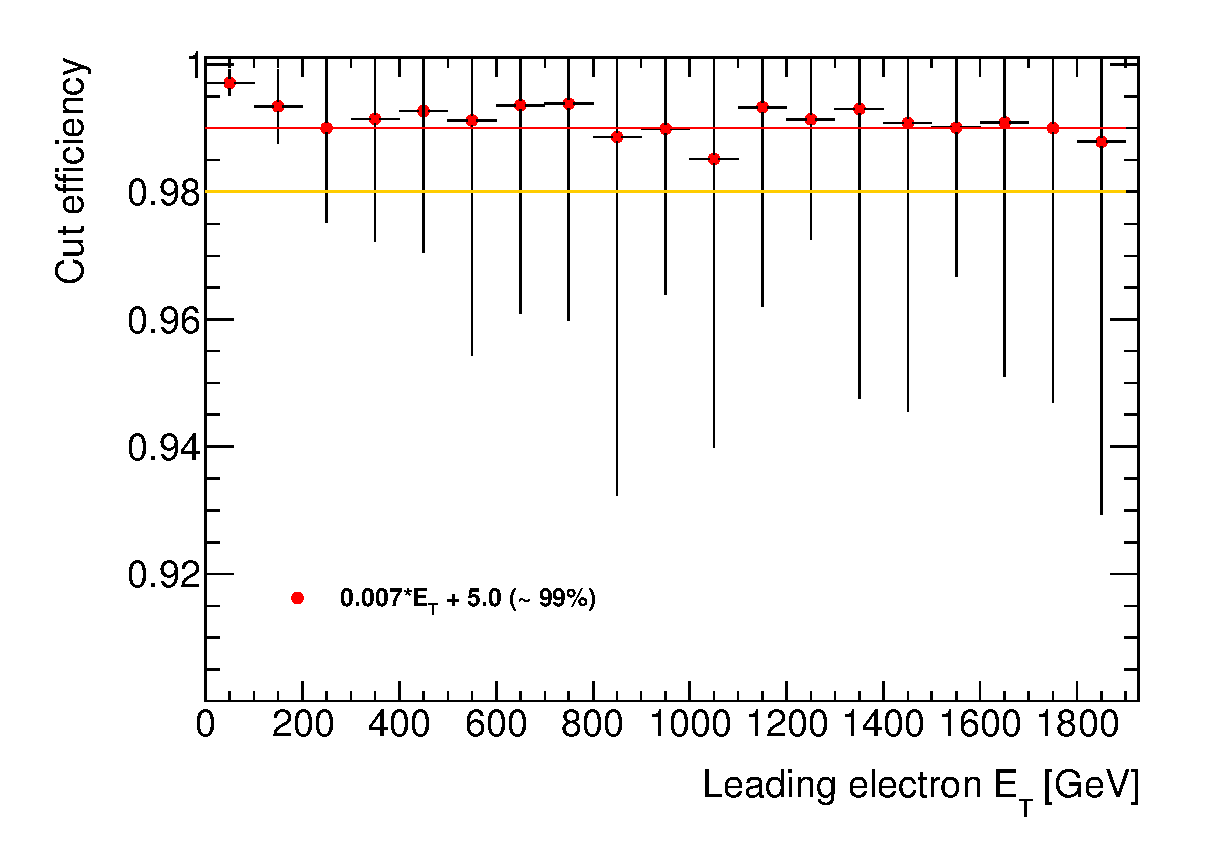
\includegraphics[scale=0.6]{images/C5_lead_iso_efficiency.eps}
      \end{center}
   \caption{Efficiency of new leading electron isolation cut on selection of signal MC. Red and orange lines indicate the 99\% and 98\% efficiency levels respectively.}
   \label{fig:C5_lead_iso_efficiency}
   \end{figure}

   \begin{figure}[h!]
      \begin{center}
      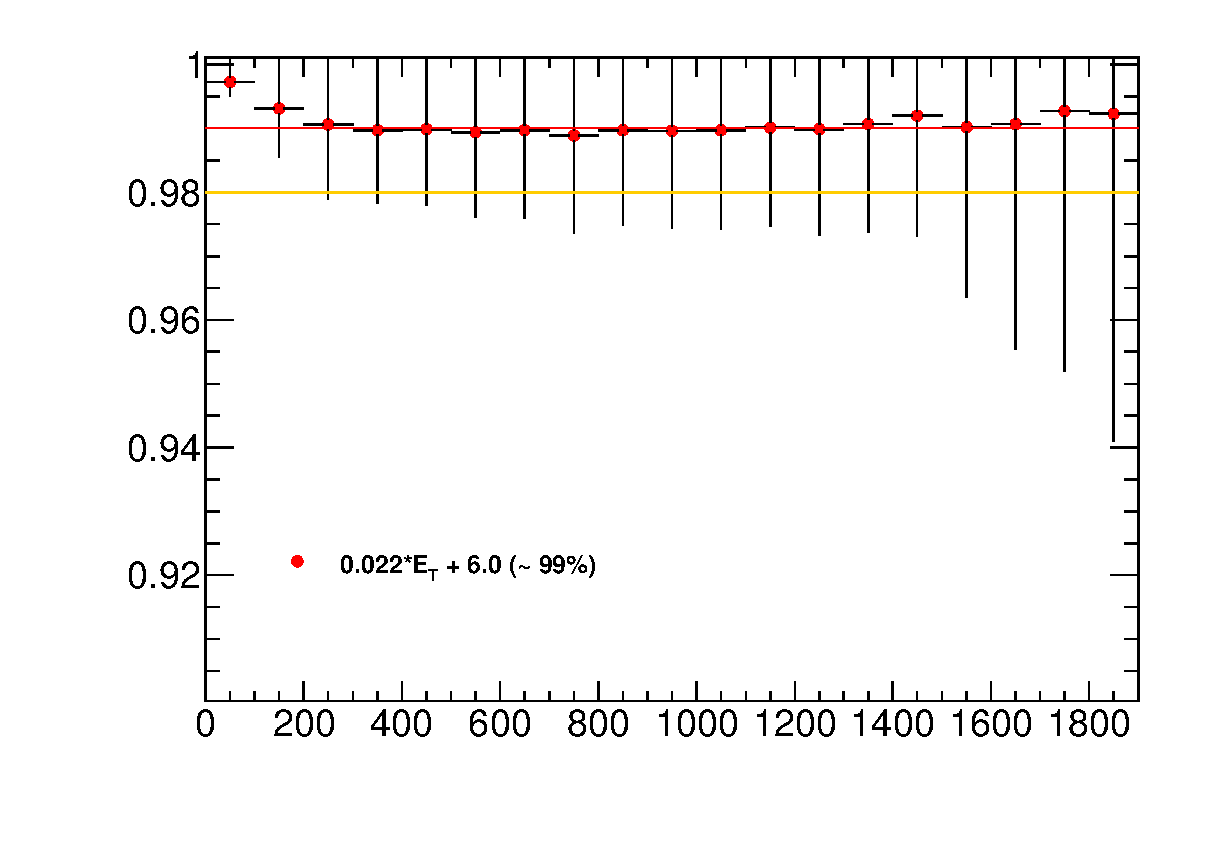
\includegraphics[scale=0.6]{images/C5_sub_iso_efficiency.eps}
      \end{center}
   \caption{Efficiency of new subleading electron isolation cut on selection of signal MC. Red and orange lines indicate the 99\% and 98\% efficiency levels respectively.}
   \label{fig:C5_sub_iso_efficiency}
   \end{figure}



\section{Opposite Sign requirement}
   %\ref{Appendix}

   The opposite sign requirement was introduced to the analysis specifically due to the use of $\cos{\theta^{*}}$ in the search. As specified in section \ref{sec:CItheory} selection of the electron and not the positron is important for the definition of $\cos{\theta^{*}}$ and if reversed would dilute the asymmetry seen in the SM and CI LR signal as seen in figure \ref{fig:theoryAFB}. The effect of swapping charge at reconstruction level comes about due to two main effects, very high energy electrons with very straight tracks getting miss identified and hard bremsstrahlung from an electron undergoing decay to an electron pair which the wrong electron getting identified. These are not a small effect at high dielectron mass ($~ 15\%$) and so the requirement is introduced to solve the issue of miss identification. The effect of both electrons being miss identified was studied and found to have only a small chance. This requirement also does a good job in the exclusion of the Multijet background reducing by 50\% throughout the signal region. The effect of the loss of acceptance attributed to this requirement is discussed in section \ref{sec:oppSign}. As this requirement has an error associated with it a systematic is introduced to accommodate this (see section \ref{sec:sys}). 


\section{Energy Scale Correction}

   During the selection process an additional correction to the energy of electrons is applied that is not included in the reconstruction. This addition comes from a study done by the ATLAS electron and photon performance group at the end of the data run calibrating energies within the Z boson peak \cite{ATLAS-CONF-2014-032}. This results in a array of energy scale corrections distributed in E$_{T}$ and $\eta$ and applied before electron selection.




\section{\texorpdfstring{Selection Acceptance $\times$ Efficiency}{Selection Acceptance x Efficiency}}

   %Figure \ref{fig:AxE} shows the acceptance $\times$ efficiency of the event selection at selecting DY MC events while 
   Table \ref{tab:eventEff} shows the efficiency of each part of the event selection. It can be seen that the opposite charge requirement causes a 7\% drop in acceptance rate in the signal region. Although a lot it can be seen in section \ref{sec:oppSign} that the effect of this drop is accommodated for by the new angular search introduced in this analysis and the reason for the selection.



   % \begin{figure}[h]
   %    \begin{center}
   %    %\includegraphics[scale=0.6]{images/}
   %    \end{center}
   % \caption{Plot showing acceptance $\times$ efficiency as a function of invariant mass for DY MC events.}
   % \label{fig:AxE}
   % \end{figure}


   \begin {table}[h]
      \begin{center}
      \begin{tabular}{|l|c|c|}
         \hline
         \hline
         Criterion & Relative Eff [\%] & Cumulative Eff [\%] \\
         \hline
         Trigger & 90.36$\pm$0.03 & 90.36$\pm$0.03 \\
         %Primary Vertex & 99.88$\pm$0.00 & 90.25$\pm$0.03 \\
         $\eta$ & 96.97$\pm$0.02 & 87.51$\pm$0.03 \\
         $p_{T}$ & 94.14$\pm$0.02 & 82.38$\pm$0.03 \\
         Shower Shape & 90.37$\pm$0.03 & 74.45$\pm$0.04 \\
         Isolation & 97.76$\pm$0.02 & 72.78$\pm$0.04 \\
         Charge & 90.43$\pm$0.03 & 65.81$\pm$0.04 \\
         \hline
         \hline
      \end{tabular}
      \caption{The efficiency of event selection on DY MC within the signal region above 400 GeV. DY MC is used due to higher statistics but is indistinguishable from signal with respect to analysis selection. Selection of number of primary vertices, of two highest $p_{T}$ electrons and the invariant mass requirement of omitted due to near 100\% acceptance on MC. Statistical errors are included only as a guide.}
      \label{tab:eventEff}
      \end{center}
   \end {table}





\newpage
\chapter{Background Estimate}

This chapter discusses methods used to estimate background processes the the signal. These background processes can be split up in to two categories; reducible and irreducible. Irreducible backgrounds consist of those background almost indistinguishable from our signal process namely clean high energy dielectron decays such as decays of the Z boson and the Drell-Yan (DY) spectrum. DY ($q\bar{q}~\rightarrow~Z/\gamma^{*}~\rightarrow~\ell^{-}\ell^{+}$) is the largest background process and also interferes with the signal processes. Another irreducible background also estimated is the Photon-Induced processes ($\gamma\gamma~\rightarrow~\ell^{-}\ell^{+}$) coming from the collision of two photons. Reducible backgrounds are those that can be reduced through event selection and three are included in this analysis. These reducible backgrounds consist of Top precesses, collisions creating single top quarks and $t\bar{t}$ events which decay to include two electrons; Diboson events, the creation of WW, WZ and ZZ events that decay in to two electron events; and finally Multi-jet \& W+jets events where one or more electron signature is faked by jet objects. All of these backgrounds are estimated via Monte Carlo generators except for the Multi-jet \& W+jets background which is estimated via a data-driven fake factor method. All background samples are summed together to create the full background estimate. MC samples are then scaled to the integrated luminosity of data collected in 2012 which is 20.3 fb$^{-1}$. Within the Z boson peak region (80 - 120 GeV) were it is known no new physics is found MC samples are scaled to data minus the multijet sample in order to rule out luminosity errors. This scale factor is found to be 1.048. Detailed below is the full derision of the background estimates ready for comparison to data.

\section{Monte Carlo samples}
   \label{sec:MC}

   Monte Carlo (MC)\footnote{Computer algorithm designed to simulate physical systems using random sampling to obtain results for a statistical physics theories such as quantum field field theories} samples are produced centrally within ATLAS using MC generators specific to  The generated events then undergo detector simulation using GEANT 4 \cite{Agostinelli2003250} which produces a data format identical to a readout from the ATLAS detector plus additional ``truth'' parameters from the original MC generation. The samples then undergo the same reconstruction as data events within ATHENA producing a MC sample ready to be analysed the same as data.\\


   {\bf\raggedright Drell-Yan}

   {\raggedright The Drell-Yan (DY) background is produced using the POWHEG + PYTHIA generator which is a next to leading order (NLO)\footnote{LO, NLO and NNLO refer to the complexity of feynman diagrams considered when calculating the cross section of an interaction} generation with POWHEG \cite{Alioli:2010xd,Alioli:2008gx} with event showering handled by PYTHIA 8 \cite{Sjostrand:2007gs}. The parton density function (PDF) used is CT10 \cite{Lai:2010vv}. A K-factor is then used in order to weight the cross-section from NLO to next to next to leading order (NNLO). This NNLO K-factor is derived using FEWZ \cite{Gavin:2010az} which uses the MSTW2008 NNLO PDF \cite{Martin:2009iq} from which a QCD+EW mass-dependent K-factor is obtained. The DY sample is split in to 16 MC truth dilepton mass bins with bin edges at (60, 120, 180, 250, 400, 600, 800, 1000, 1250, 1500, 1750, 2000, 2250, 2500, 2750, 3000) GeV. The first bin from 60 - 120 GeV is a very high statistics sample providing a low statistical uncertainty for the region used for scaling MC in the Z boson peak.} \\


   {\bf\raggedright Photon-Induced}

   {\raggedright The Photon-Induced (PI) fraction is estimated via PYTHIA 8 \cite{Sjostrand:2007gs} generator with the LO PDF MRST2004QED \cite{Martin:2004dh}. This sample is split in to 5 dilepton mass bins with bin edges at (60, 200, 600, 1500, 2500) GeV.}\\


   {\bf\raggedright Diboson}

   {\raggedright The Diboson MC sample is produced using HERWIG 6.510 \cite{Corcella:2002jc} with the LO PDF CTEQ6L1 \cite{Pumplin:2002vw}. The sample with split in to the three process, WW, WZ and ZZ, with each process split in to 3 mass-binned samples with bin edges of (60, 400, 1000) GeV. The sample is then scaled to NLO in a mass-independent way using MCFM \cite{Campbell:2010ff} with the PDF MSTW2008 NLO \cite{Martin:2009iq}}\\

   {\bf\raggedright Top}

   {\raggedright The top sample is estimated using MC@NLO 3.41 \cite{Frixione:2008ym} with NLO PDF CT10 \cite{Lai:2010vv} to generate matrix elements with JIMMY 4.31 \cite{Butterworth:1996zw} describing parton interactions and HERWIG \cite{Corcella:2002jc} deriving the underlying event and parton showers. Both $t\bar{t}$ and single Top processes are generated in two inclusive samples. A NNLO QCD K-factor is also derived using Top++ 2.0 \cite{Czakon:2013goa,Cacciari:2011hy}. The top sample also undergoes a fit at high mass where the MC has low statistics. A dijet function ($c_{0}x^{c_{1}} x^{c_{2}\log{x}}$) is used to fit between 200 - 700~GeV then the sample is cut at 500~GeV above which the dijet fit is used.}


\subsection{MC Corrections}
   \label{sec:correc}

   Corrections are applied to MC sample due to several factors including unknown run conditions within the ATLAS detector due to MC samples being run before the LHC run as well as known inefficiencies in the reconstruction of MC events. Below are listed all of the corrections which are applied on an event by even basis during the analysis of MC samples.\\


   {\bf\raggedright Pile-up Correction}

   {\raggedright Pile-up (PU) is the number of simultaneous proton-proton interactions within an event. MC samples are produced with a broad range of PU values which then get weighted according to run conditions within the detector. PU conditions can change throughout data taking and so the PU correction is specified for a particular set of ATLAS data. The distributions MC is weighted to can be seen in figure \ref{fig:pu}.}\\

   {\bf\raggedright Vertex Position Reweighting}

   {\raggedright Vertex position hard to predict pre-run and can therefore be weighted later once run conditions are known. This correction is not widely used within ATLAS due to its minimal effect however it was found to add better data background agreement to the $\cos{\theta^{*}}$ distribution within the scaling and control region. The vertex position reweighting was found to have a minimal effect on the invariant mass distribution.}\\

   {\bf\raggedright Energy Smearing Correction}

   {\raggedright The energy smearing correction is used to better estimate the energy of electron signatures. This correction is derived from a Z peak calibration study \cite{ATLAS-CONF-2014-032} done within the ATLAS electron photon performance group and matches MC to data. These corrections provide a $\eta$ and E$_{T}$ dependent smearing value applied to electron energy before electron selection.}\\

   {\bf\raggedright Electron Efficiency Scale Factor}

   {\raggedright The electron photon performance group also identified inefficiencies in electron reconstruction and identification. These form a set of scale factors applied in bins of E$_{T}$ and $\eta$ after event selection.}\\


   {\bf\raggedright Isolation and Trigger Scale Factor}

   {\raggedright Data/MC comparison for the isolation selections and the trigger requirements highlighted minor differences between data and MC. The differences were found to be below 1\% yet a uniform scale factor accommodating this were applied after event selection for completeness.}




\section{Fake Factor Multi-Jet Estimate}
   \label{sec:FFmethod}

One of the major sources of background to di-electron signals are di-jets or electron+jets (mainly W+jets) events where one or both selected leptons are jets faking electron signatures. The method for estimating this background, described here, is a ``fake factor'' or ``matrix-method''. This is a data-driven method where electrons are selected by a tight ($N_{tight}$) and loose ($N_{loose}$) selection. The tight selection is the standard electron selection used in this analysis while the loose selection has no isolation requirement and must only pass a loose++ egamma definition (see section \ref{sec:ReconElec}) with no track matching criteria. $N_{tight}$ is therefore by design a subset of $N_{loose}$. Two more hidden values are also assigned $real$ and $fake$ referring to true source of each electron. This gives us two coefficients to determine from data.

\begin{equation} \label{eq:fakeRate}
   f~=~\frac{N^{fake}_{tight}}{N^{fake}_{loose}} \qquad \qquad r~=~\frac{N^{real}_{tight}}{N^{real}_{loose}}
\end{equation}

The fake rate $f$ denotes the probability that a $fake$ electron which passes the loose requirement also passes tight while $r$ refers to the probability that a $real$ electron which passes the loose requirement also passes the tight.
Reconstructed events are split in to two distinct groups, tight($T$), and loose while failing tight($L$), where $Tight$ is now no longer a subset of $Loose$. This allows the reconstructed events to be related to the underling truth events via a matrix of fake rates shown in equation~\ref{eq:mainFakeMatrix}.

\begin{equation} \label{eq:mainFakeMatrix}
   \begin{pmatrix}
      N_{TT} \\
      N_{TL} \\
      N_{LT} \\
      N_{LL} \\
   \end{pmatrix}
   =
   \begin{pmatrix}
      r_{1}r_{2} & r_{1}f_{2} & f_{1}r_{2} & f_{1}f_{2} \\
      r_{1}(1-r_{2}) & r_{1}(1-f_{2}) & f_{1}(1-r_{2}) & f_{1}(1-f_{2}) \\
      (1-r_{1})r_{2} & (1-r_{1})f_{2} & (1-f_{1})r_{2} & (1-f_{1})f_{2} \\
      (1-r_{1})(1-r_{2}) & (1-r_{1})(1-f_{2}) & (1-f_{1})(1-r_{2}) & (1-f_{1})(1-f_{2}) \\
   \end{pmatrix}
   \begin{pmatrix}
      N_{RR} \\
      N_{RF} \\
      N_{FR} \\
      N_{FF} \\
   \end{pmatrix}
\end{equation}

The first index in equation~\ref{eq:mainFakeMatrix} refers to the highest $p_{T}$ electron while the second index refers to the second highest $p_{T}$ electron. So $N_{LT}$ indicates the reconstructed events with highest $p_{T}$ electron only passing the $Loose$ selection while the second highest $p_{T}$ electron passes $Tight$ selection. The indices 1 and 2 refer to fake rates ($f$) and efficiencies ($r$) on leading and sub-leading electrons respectively.

The interesting part for this study is the contribution to $N_{TT}$ coming from sources other than $N_{RR}$, these can be seen in equation~\ref{eq:multijet}.

\begin{align} \label{eq:multijet}
   N^{\ell+jets}_{TT}~&=~r_{1}f_{2}N_{RF}~+~f_{1}r_{2}N_{FR} \nonumber \\
   N^{di-jets}_{TT}~&=~f_{1}f_{2}N_{FF} \nonumber \\
   N^{\ell+jets~\&~di-jets}_{TT}~&=~r_{1}f_{2}N_{RF}~+~f_{1}r_{2}N_{FR}~+~f_{1}f_{2}N_{FF} 
\end{align}

This function however contains hidden variables and so equation~\ref{eq:mainFakeMatrix} is inverted to derive a better formalism.

\begin{equation}
   \begin{pmatrix}
      N_{RR} \\
      N_{RF} \\
      N_{FR} \\
      N_{FF} \\
   \end{pmatrix}
   = \alpha
   \begin{pmatrix}
      (f_{1}-1)(f_{2}-1) & (f_{1}-1)f_{2} & f_{1}(f_{2}-1) & f_{1}f_{2} \\
      (f_{1}-1)(1-r_{2}) & (1-f_{1})r_{2} & f_{1}(1-r_{2}) & -f_{1}r_{2} \\
      (r_{1}-1)(1-f_{2}) & (1-r_{1})f_{2} & r_{1}(1-f_{2}) & -r_{1}f_{2} \\
      (1-r_{1})(1-r_{2}) & (r_{1}-1)r_{2} & r_{1}(r_{2}-1) & r_{1}r_{2} \\
   \end{pmatrix}
   \begin{pmatrix}
      N_{TT} \\
      N_{TL} \\
      N_{LT} \\
      N_{LL} \\
   \end{pmatrix}
\end{equation}
where,
\begin{equation}
   \alpha~=~\frac{1}{(r_{1}-f_{1})(r_{2}-f_{2})}
\end{equation}

The fraction of selected events with at least one fake is then given by equation \ref{eq:multijet} resulting in equation \ref{eq:mainFakeResult1}.

\begin{equation} \label{eq:mainFakeResult1}
\begin{aligned}
   N^{\ell+jets~\&~di-jets}_{TT}~&=&~\alpha r_{1}f_{2}[(f_{1}-1)(1-r_{2})N_{TT}~+~(1-f_{1})r_{2}N_{TL}~&+~f_{1}(1-r_{2})N_{LT}~-~f_{1}r_{2}N_{LL}] \\
      &~+&~\alpha f_{1}r_{2}[(r_{1}-1)(1-f_{2})N_{TT}~+~(1-r_{1})f_{2}N_{TL}~&+~r_{1}(1-f_{2})N_{LT}~-~r_{1}f_{2}N_{LL}] \\
      &~+&~\alpha f_{1}f_{2}[(1-r_{1})(1-r_{2})N_{TT}~+~(r_{1}-1)r_{2}N_{TL}~&+~r_{1}(r_{2}-1)N_{LT}~+~r_{1}r_{2}N_{LL}] 
\end{aligned}
\end{equation}

\begin{equation} \label{eq:mainFakeResult2}
\begin{aligned}
   =\alpha[r_{1}f_{2}(f_{1}-1)(1-r_{2})~+~f_{1}r_{2}(r_{1}-1)(1-f_{2})~+~f_{1}f_{2}(1-r_{1})(1-r_{2})]N_{TT} \\
   +~\alpha f_{2}r_{2}[r_{1}(1-f_{1})~+~f_{1}(1-r_{1})~+~f_{1}(r_{1}-1)]N_{TL} \\
   +~\alpha f_{1}r_{1}[f_{2}(1-r_{2})~+~r_{2}(1-f_{2})~+~f_{2}(r_{2}-1)]N_{LT} \\
   -~\alpha f_{1}f_{2}r_{1}r_{2}N_{LL}
\end{aligned}
\end{equation}

Equation \ref{eq:mainFakeResult2} shows the derived formula relating the multi-jet background to fake rates, efficiencies and four independent samples $N_{TT}$, $N_{TL}$, $N_{LT}$ and $N_{LL}$ which can be selected from data. Following are the details of this method used on the full $20~fb^{-1}$ of integrated luminosity from ATLAS's 2012 run. This method was developed centrally in the resonant analysis which the author then applied and tested for this non-resonant analysis.


\subsection{Real Electron Efficiency Estimation}

The real electron efficiency is defined in equation~\ref{eq:fakeRate} as $r~=~N^{real}_{tight}/N^{real}_{loose}$. This is determined from MC using a mass binned Drell-Yan sample. The efficiencies are found for both the leading and sub-leading electrons and binned in 8 $p_{T}$ and three eta bins of $|\eta|<1.37$ (barrel), $1.52<|\eta|<2.01$ and $2.01<|\eta|<2.47$ (endcap). The efficiency is distributed between $90$ - $96\%$ as is shown in figure \ref{fig:realEff}.

   \begin{figure}[h]
      \begin{center}
      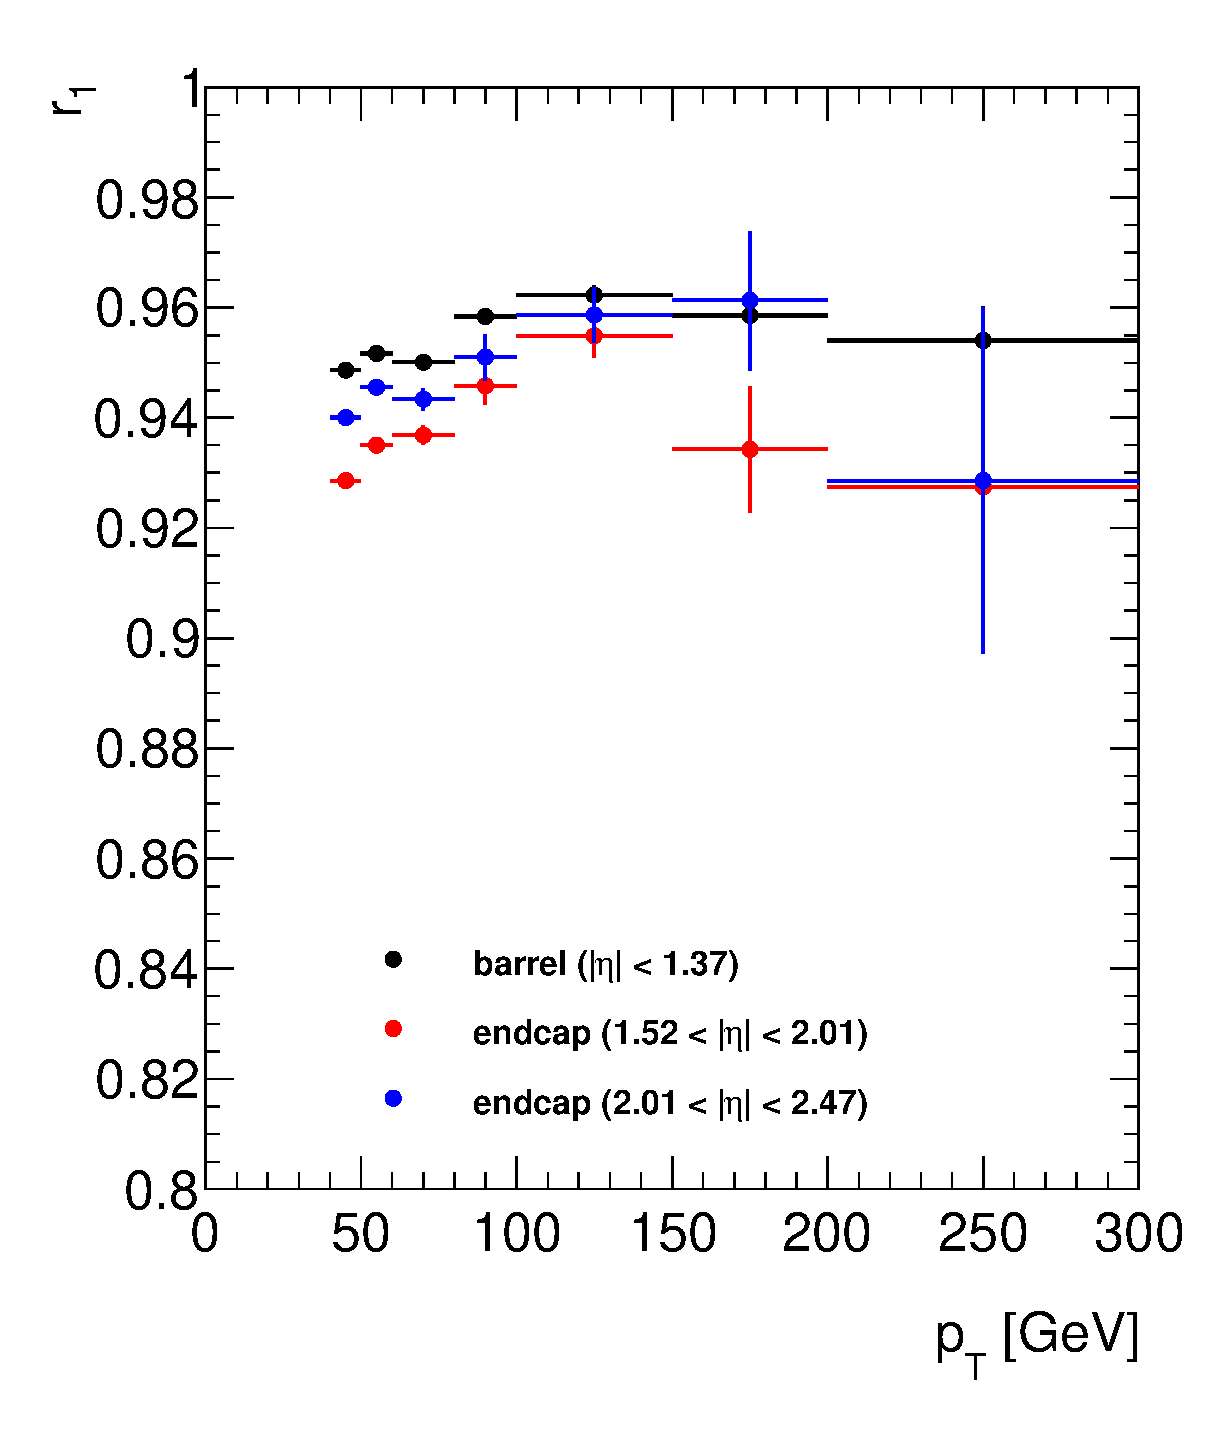
\includegraphics[width=0.48\linewidth]{images/r1.eps}
      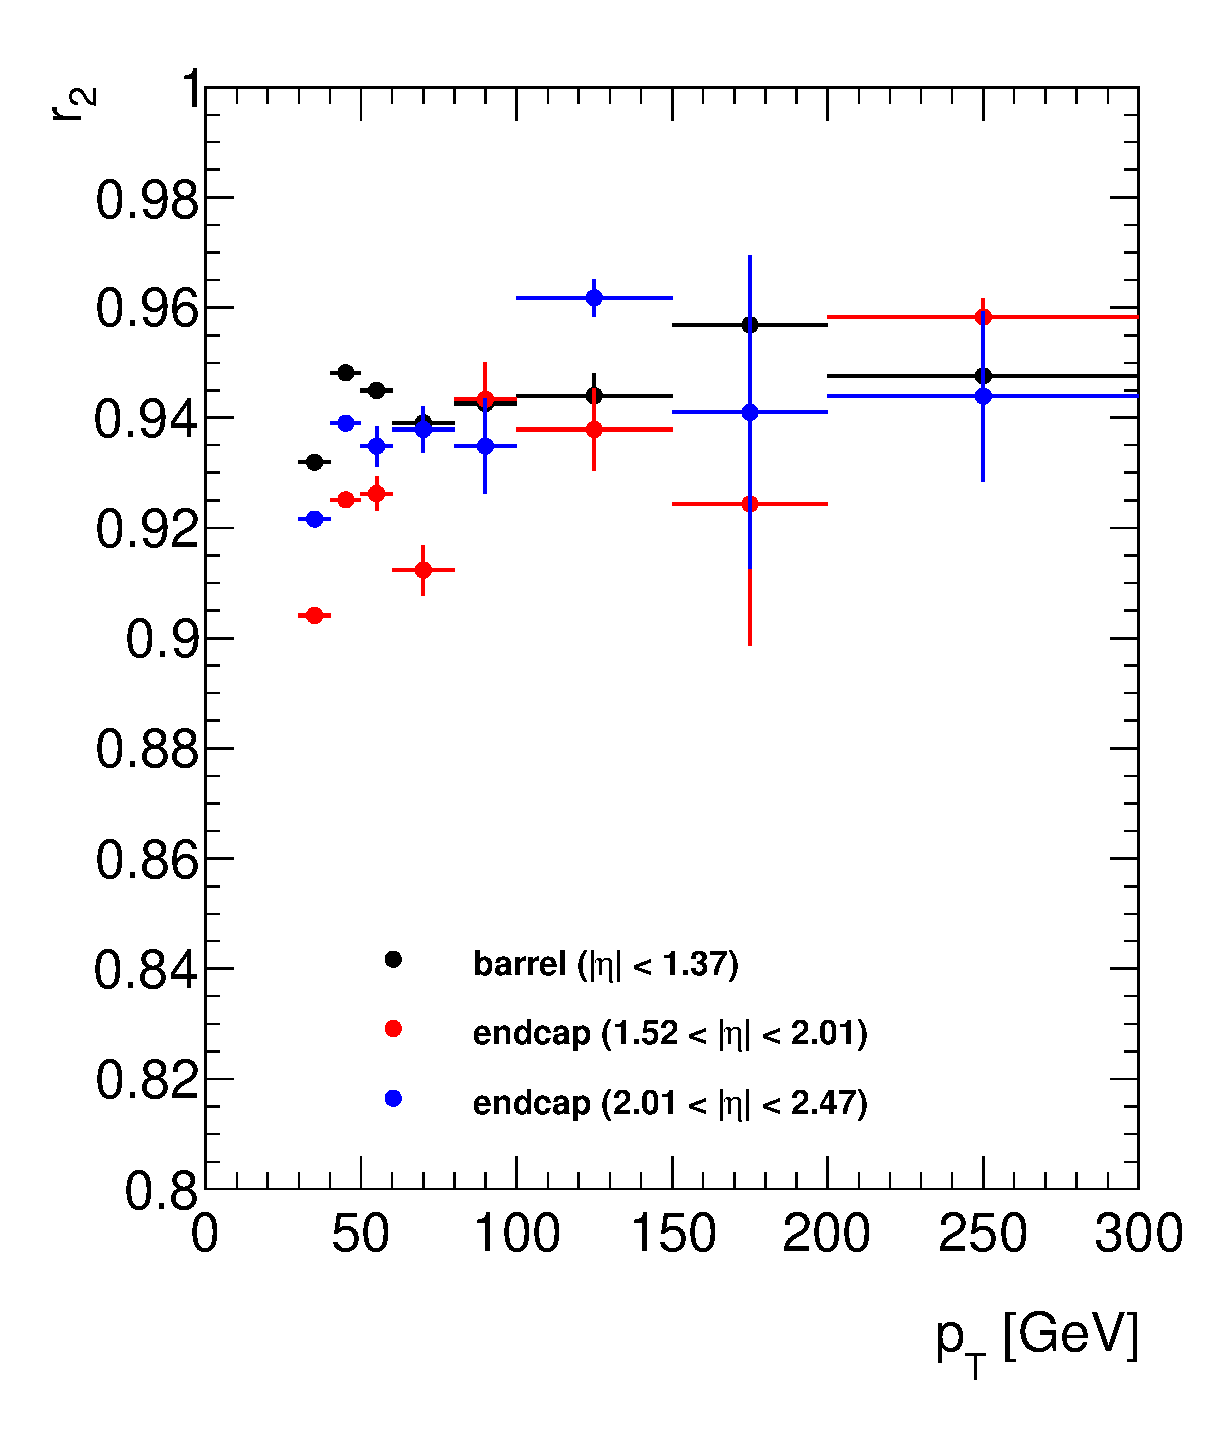
\includegraphics[width=0.48\linewidth]{images/r2.eps}
      \end{center}
   \caption{Real electron efficiencies obtained from Drell-Yan MC and binned in $p_{T}$ and three coarse $\eta$ bins covering the barrel and two endcap regions. Efficiencies for leading electrons are shown on the left while those for subleading electron are on the right.}
   \label{fig:realEff}
   \end{figure}



\subsection{Fake Electron Rate Estimation}

The default method selected for analysing the fake rates is a single object method selection on the jet stream data. This has the advantage of more statistics and a higher energy reach compared to methods such as using tag and probe on the egamma stream data.
An array of triggers are used for selecting suitable events with many different thresholds. 
%EF\_jX\_a4chad (where X = 25, 35, 45, 55, 80, 110, 145, 180, 220, 280, 360). 
Events are associated to groups with the lowest trigger threshold they pass as each trigger has a different prescale. Objects are selected with jet algorithms and then matched to objects in the egamma stream with a $\Delta R~<~0.1$. Two further steps are taken to suppress real electrons from W decays and real Drell-Yan events. A veto of $E_{Tmiss}~>~25~GeV$ is introduced to combat the former while events with two medium++ or loose++ electrons with $|m_{tag~\&~probe}-91~GeV|~<~20~GeV$ are vetoed to counter the real Drell-Yan.

The fake rate as defined in equation~\ref{eq:fakeRate} ($f~=~N^{fake}_{tight}/N^{fake}_{loose}$) with the $N^{fake}_{tight}$ and $N^{fake}_{loose}$ distributions selected using the standard event selection on the matched egamma objects.
Due to the different prescales of each trigger a separate set of fake rates are calculated for each trigger, these are then combined as a weighted average of all fake rates. Figure \ref{fig:fakeRates} shows the distribution of fake rates for leading and subleading fakes. These are distributed between 3 - $20\%$. This calculation of fake rates was completed in the resonant analysis group and the results were carried over to this analysis. The differences in the event selection were found to not effect the results.

   \begin{figure}[h]
      \begin{center}
      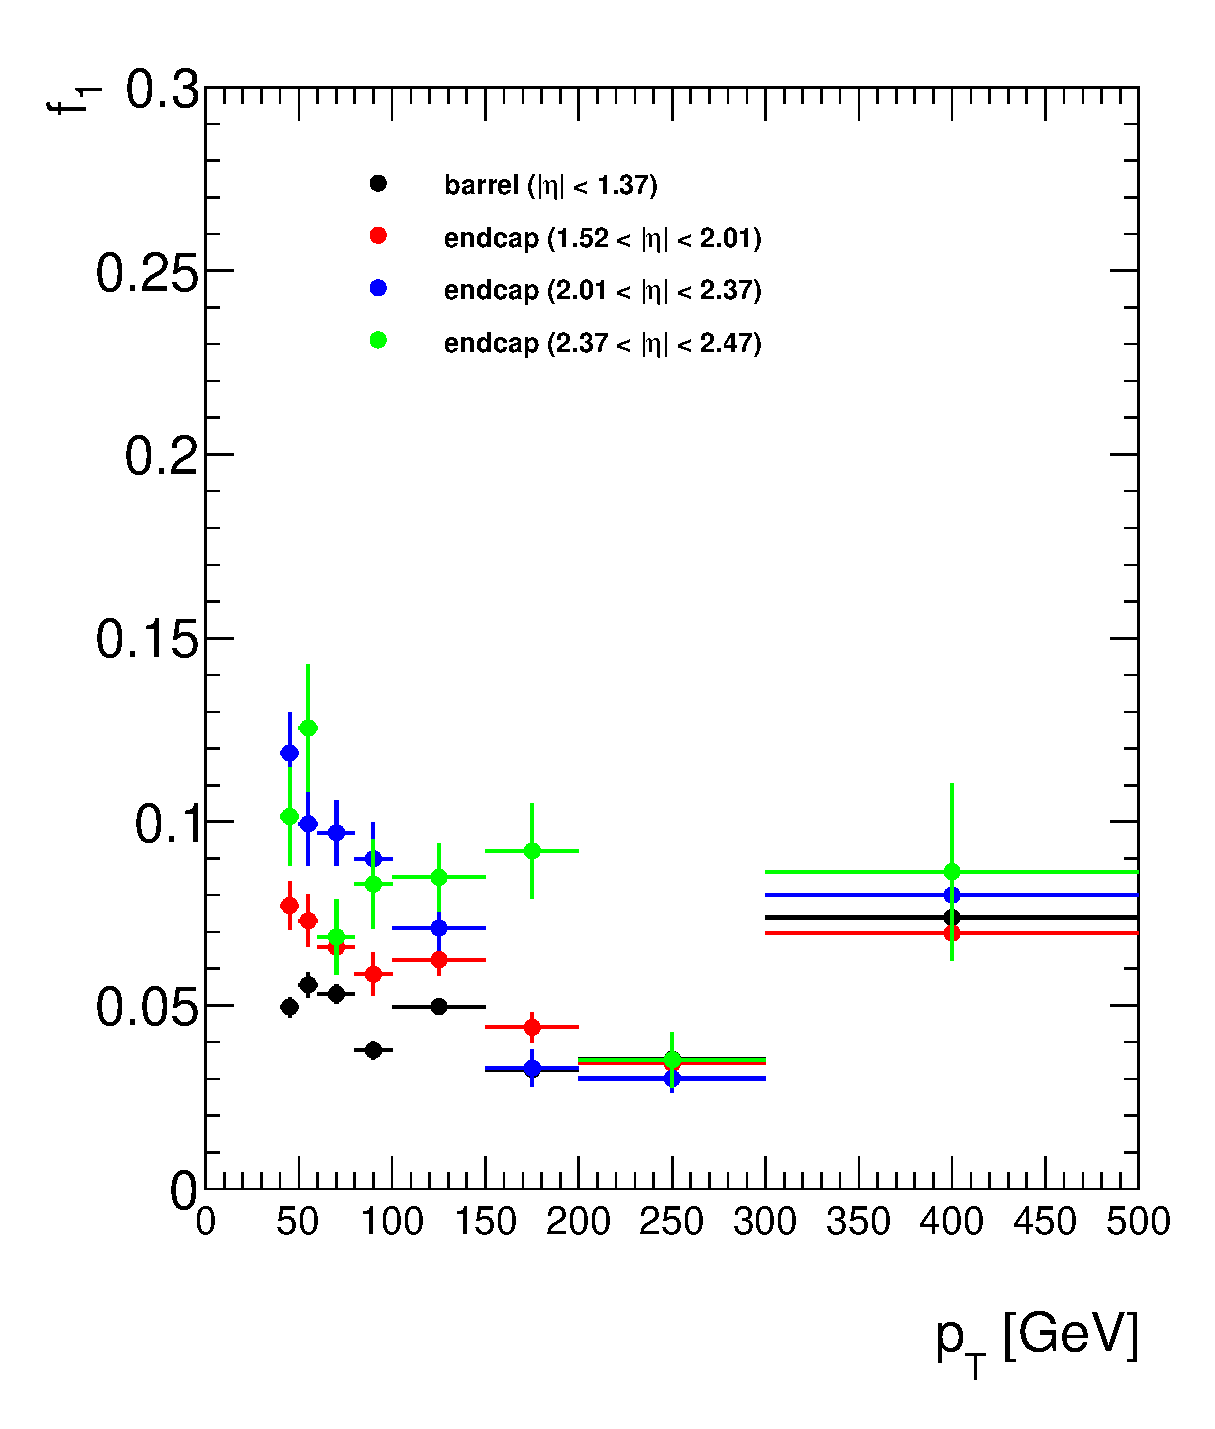
\includegraphics[width=0.48\linewidth]{images/f1.eps}
      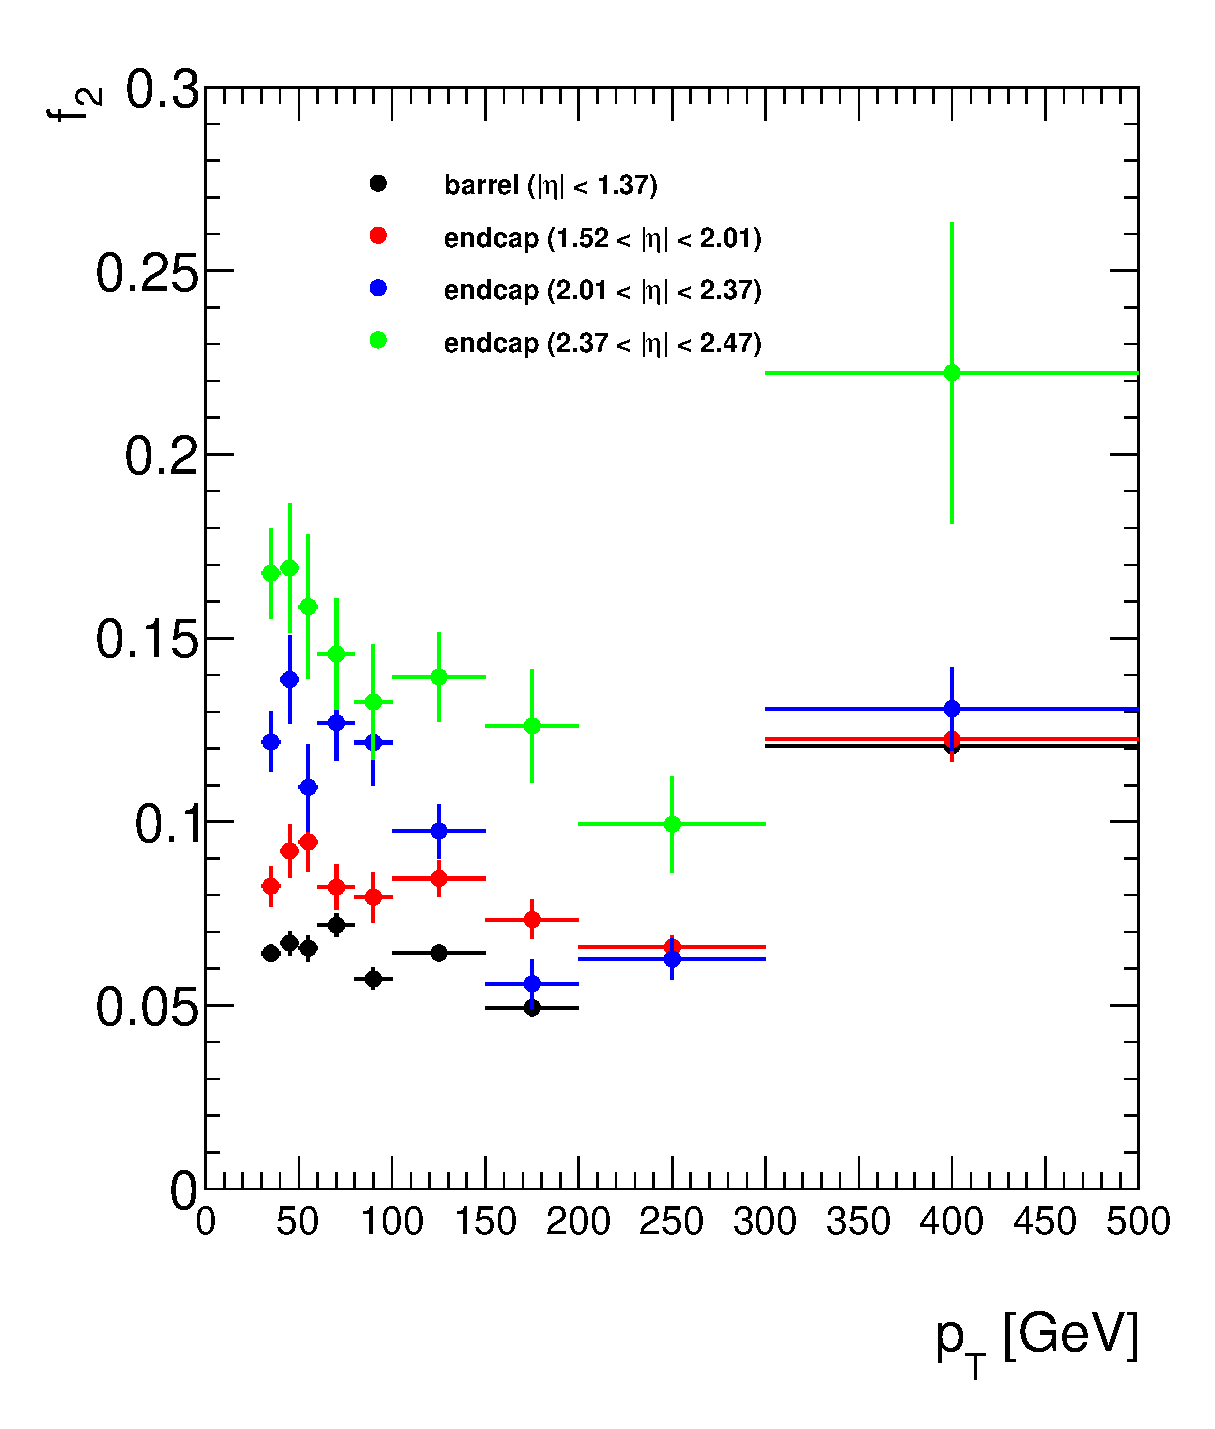
\includegraphics[width=0.48\linewidth]{images/f2.eps}
      \end{center}
   \caption{Fake rates obtained from data and binned in $p_{T}$ and four coarse $\eta$ bins covering the barrel and three endcap regions. Fake rates for leading electrons are shown on the left while those for subleading electron are on the right.}
   \label{fig:fakeRates}
   \end{figure}




\subsection{Properties of Multi-Jet Background}

In order to compose the final sample events are organised by the distributions $N_{TT}$, $N_{TL}$, $N_{LT}$ or $N_{LL}$ and weights are applied according to each electrons $p_{T}$, $\eta$ with respect to equation~\ref{eq:mainFakeResult2} and the corresponding efficiencies and fake rates. 
Figure \ref{fig:N_dist} shows these distributions before the efficiencies and fake rates are applied to weight to the final background prediction. In addition to these steps an extra fit is then applied at low invariant mass due to contamination due to the Z boson peak. This method is not suited to predicting the Multi-Jet background in the Z boson peak region and so a fit is obtained between 120 GeV and 400 GeV and stitched from 110 GeV and below. This gives a good estimate to the integral in this region for use in scaling MC's to luminosity but is not predicted to be good at predicting other variables in this region. At high-mass statistics of the sample decline and so an additional fit is made a high mass with the lower edge of the fit varied between 425 and 600 GeV and the upper edge from 700 to 1200 GeV, with the stitching point at 500 GeV.

   \begin{figure}[h]
      \begin{center}
      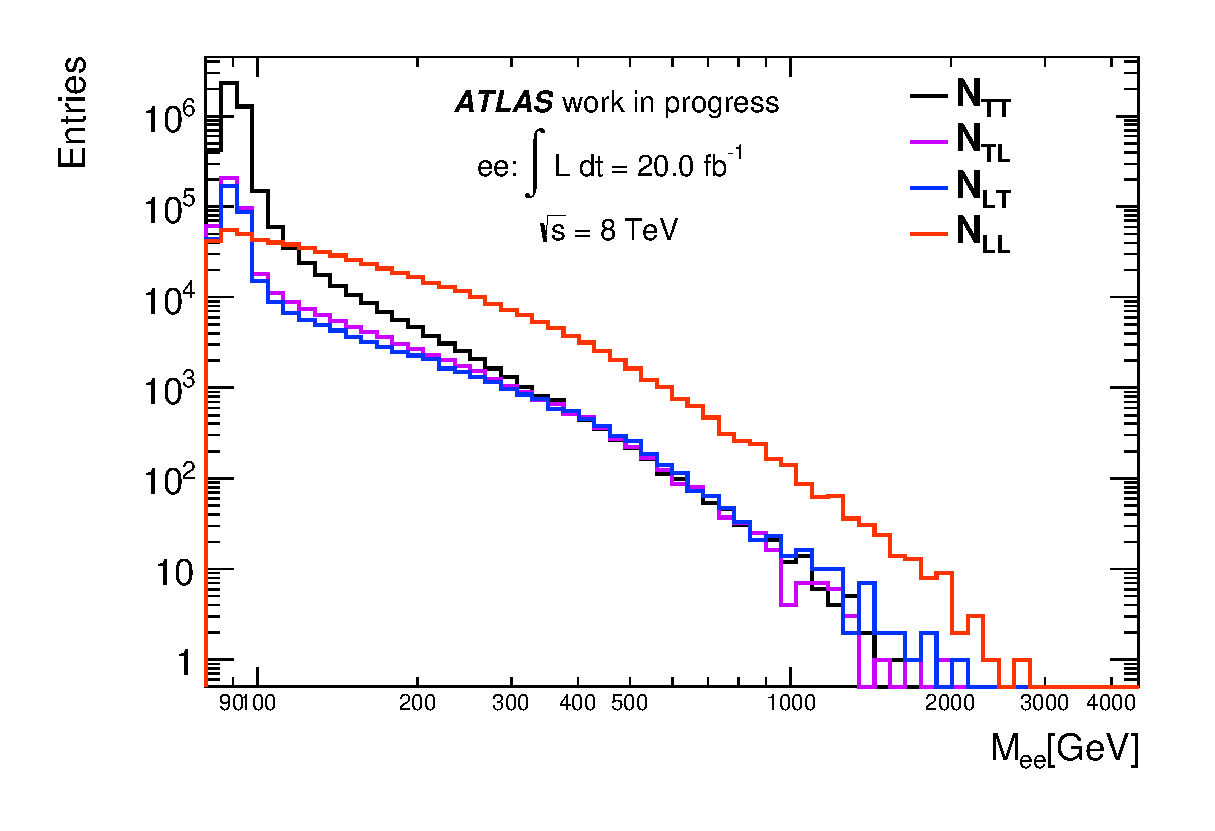
\includegraphics[width=0.98\linewidth]{images/N_distributions.eps}
      \end{center}
   \caption{Distribution of $N_{TT}$, $N_{TL}$, $N_{LT}$ and $N_{LL}$ from data with no weightings applied.}
   \label{fig:N_dist}
   \end{figure}






\subsection{Other Methods and Estimation of Error}
   \label{sec:MJerror}


Two other methods and variations upon them were used to test the validity of this method as well as estimate the systematic error of this background estimation procedure. These two methods are both tag and probe measurements; one on the jet stream of data, and another on the egamma stream where the method is more an ``inverse'' tag and probe with the selection of a tag with high probability of being a jet. Variations are also made on the method by assuming $r_{1}$ and $r_{2} = 1.0$ in all cases as well as changing the definition of loose but fail tight. These variations simplify the equations slightly but the method remains the same. Variations compared to the default method used to obtain the estimation were found to vary between $\pm$ 20\% throughout the invariant mass distribution. The systematic uncertainty of the multi-jet estimate was therefore taken to be a flat $20\%$ throughout the distribution.





\section{Total Background Estimate}

The total stacked summation of all the backgrounds, after all corrections and scaling within the Z peak have been applied, can be seen in figure \ref{fig:totalBKG}.


   \begin{figure}[h]
      \begin{center}
      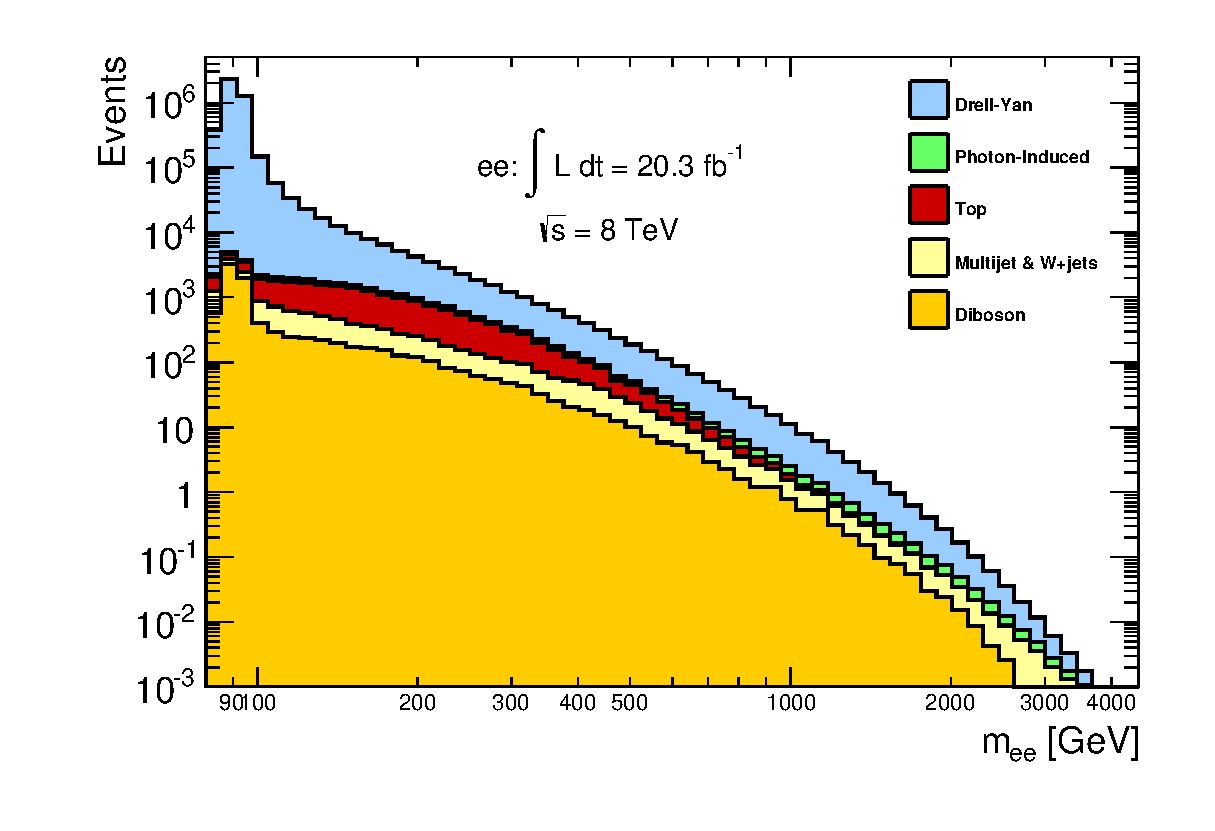
\includegraphics[width=0.98\linewidth]{images/invMass_bkgonly.eps}
      \end{center}
   \caption{Combined background samples scaled to data in the Z peak.}
   \label{fig:totalBKG}
   \end{figure}







\newpage
\chapter{Signal and Results}

This chapter discusses the MC generators used to model signal distributions and how these are parametrised for input to the statistical analysis. This is followed by the results of the data background comparison looking for any sign of new physics signal.

\section{Signal Monte Carlo}

	All signal MC is produced in the same way as the background MC and then summed with the other background predictions to arrive at the full signal prediction. Each sample also gets scaled by the same factor as the background MC from the Z peak scaling. \\


	\subsection*{Contact Interaction}

	Contact Interaction samples are generated using PYTHIA 8 \cite{Sjostrand:2007gs} with the leading order PDF MSTW2008LO \cite{Martin:2009iq}. The CI MC samples also have a K-factor applied that is derived in the same way as the DY K-factor but scaling from LO to NNLO (see section \ref{sec:MC}). A selection of $\Lambda$ values was chosen to cover the reach in new physics for all formalisms of the model (LL, LR and RR). This constituents signals for $\Lambda$ = 7, 10, 14, 20 and 28 TeV. For each of these working points parametrisations of constructive and destructive interference and LL, LR and RR models are all generated. This makes 6 parametrisations with 5 $\Lambda$ values produced for each one. Each MC sample is composed of three dilepton mass binned samples above 300 GeV in order to maintain statistics. Below 300 GeV negligible new physics is predicted and so the SM DY prediction is used below this point. 
	Because this MC sample is LO a PYTHIA 8 LO DY sample is also produced. This sample models the DY in the same way as the signal samples allowing you to subtract it from the signal samples to leave a pure new physics signal sample. This signal sample can then be added to the other background samples including the background MC DY sample (seen in section \ref{sec:MC}) to give a full signal prediction with a more consistent and higher statistics DY sample.


	\subsection*{ADD}

	The ADD samples used are produced using the SHERPA 1.4.1 \cite{1126-6708-2009-02-007} generator and NLO PDF CT10 \cite{Lai:2010vv}. Only two formalisms are produced as limits for other formalisms can be converted from the GRW one. The only formalism this is not possible for is HLZ ($n$ = 2). For these 2 formalisms 4 values of M$_{s}$ are generated of M$_{s}$ = 4.75, 4.0, 3.75 and 3.5 TeV. Again 3 dilepton mass bins are used above 300 GeV with the SM DY replacing the distribution below this. Also, like the CI samples, a specific DY only SHERPA sample is produced which is them subtracted from the signal samples so the background MC DY can be used.



\section{Signal Parametrisation}
	\label{sec:parm}

	Each formalism of the CI and ADD model is parametrised according to the form of their individual cross-sections (Eq's \ref{eq:DiffCross} and \ref{eq:ADDcs}) and as a function of their parameter of interest ($\Lambda$, M$_{s}$). The parametrisations are a prediction of number of expected events $N_{\text{exp}}$ where the parameter of interest ($\Lambda$, M$_{s}$) at $\infty$ equates to no signal and just the SM background prediction, these can be seen in equations \ref{eq:CIparm} and \ref{eq:ADDparm}. 

	\begin{equation}
        N_{\text{exp}}(\Lambda)~=~c_{0} + \frac{c_{1}}{\Lambda^{2}} + \frac{c_{2}}{\Lambda^{4}}
        \label{eq:CIparm}
    \end{equation}

    \begin{equation}
        N_{\text{exp}}(\text{M}_{s})~=~c_{0} + \frac{c_{1}}{\text{M}_{s}^{4}} + \frac{c_{2}}{\text{M}_{s}^{8}}
        \label{eq:ADDparm}
    \end{equation}

	Here $c_{0}$ refers to the SM background prediction while $c_{1}$ and $c_{2}$ show the dependence of the scale of new physics on number of expected events. Each formalism gets parametrised in every search bin. These search bins are described at the start of chapter \ref{ch:stat} while the parametrisations can be seen in figure \ref{fig:CIparm} for every CI mass bin. The full list of all of the parametrisations used can be found in appendix \ref{ap:parm}.


	\begin{figure}[h!]
	    \begin{center}
	    	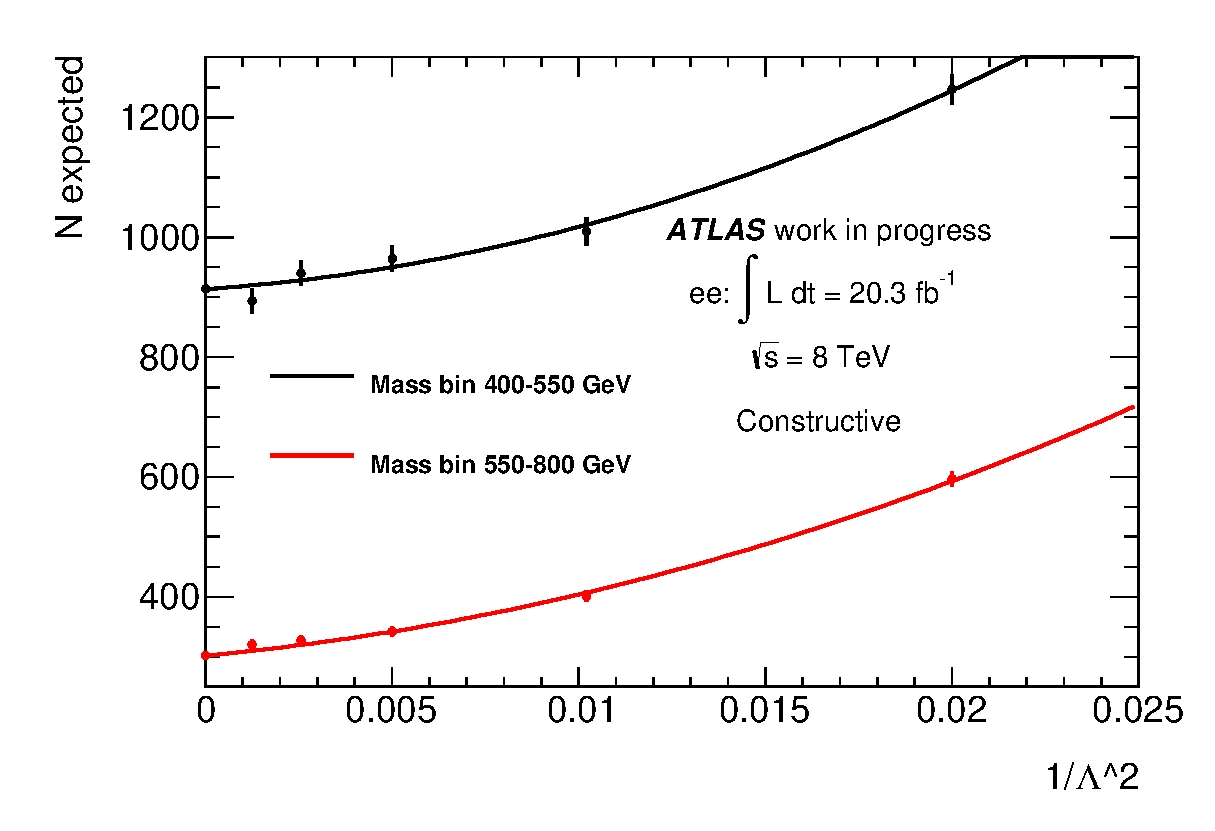
\includegraphics[width=0.49\linewidth]{images/parametrisations/NexpFits_minus_elec_lowmass.eps}
	    	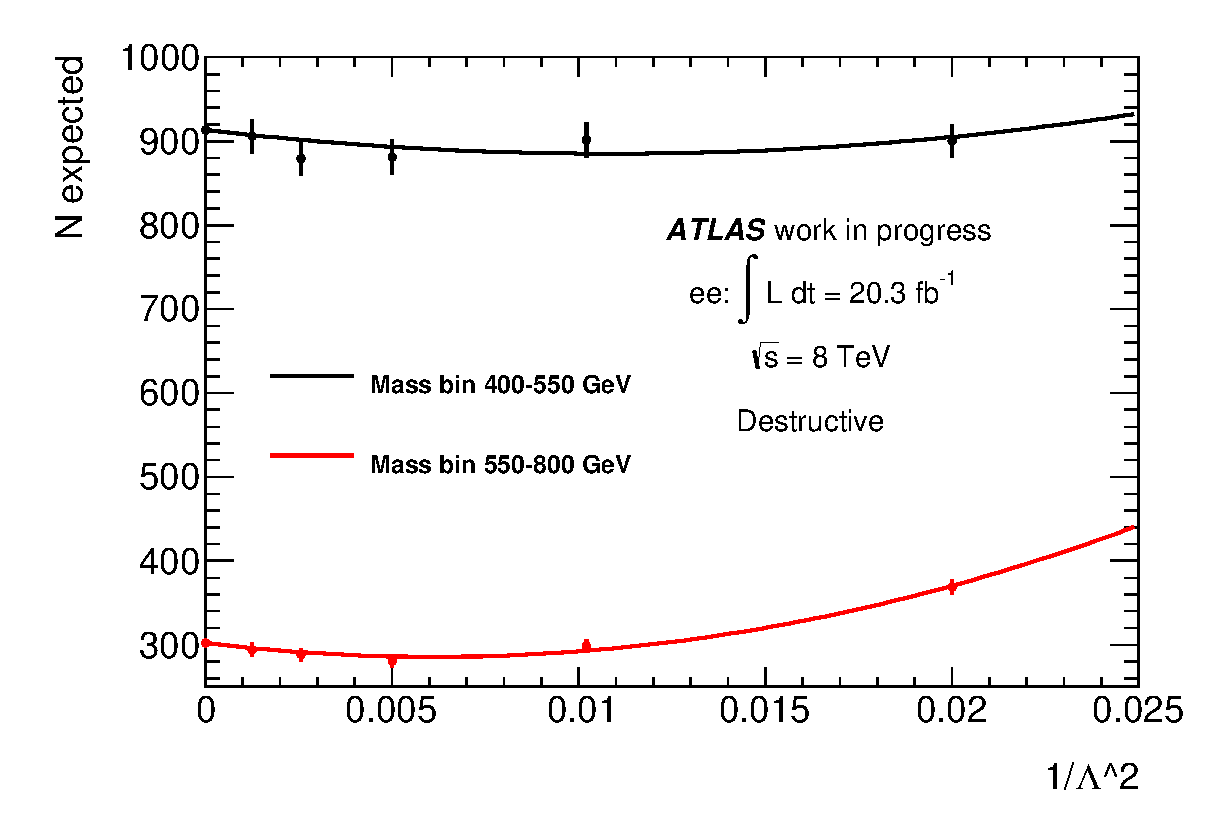
\includegraphics[width=0.49\linewidth]{images/parametrisations/NexpFits_plus_elec_lowmass.eps} \\
	    	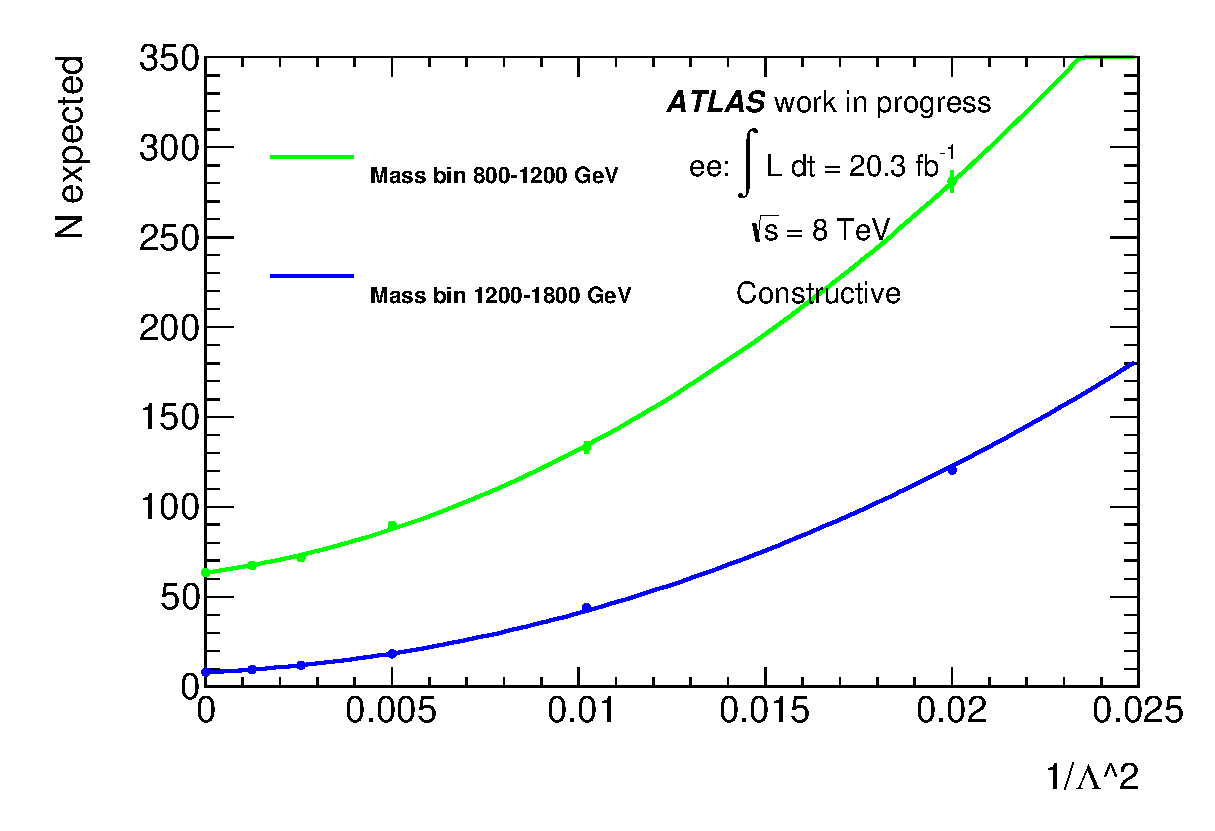
\includegraphics[width=0.49\linewidth]{images/parametrisations/NexpFits_minus_elec_midmass.eps}
	    	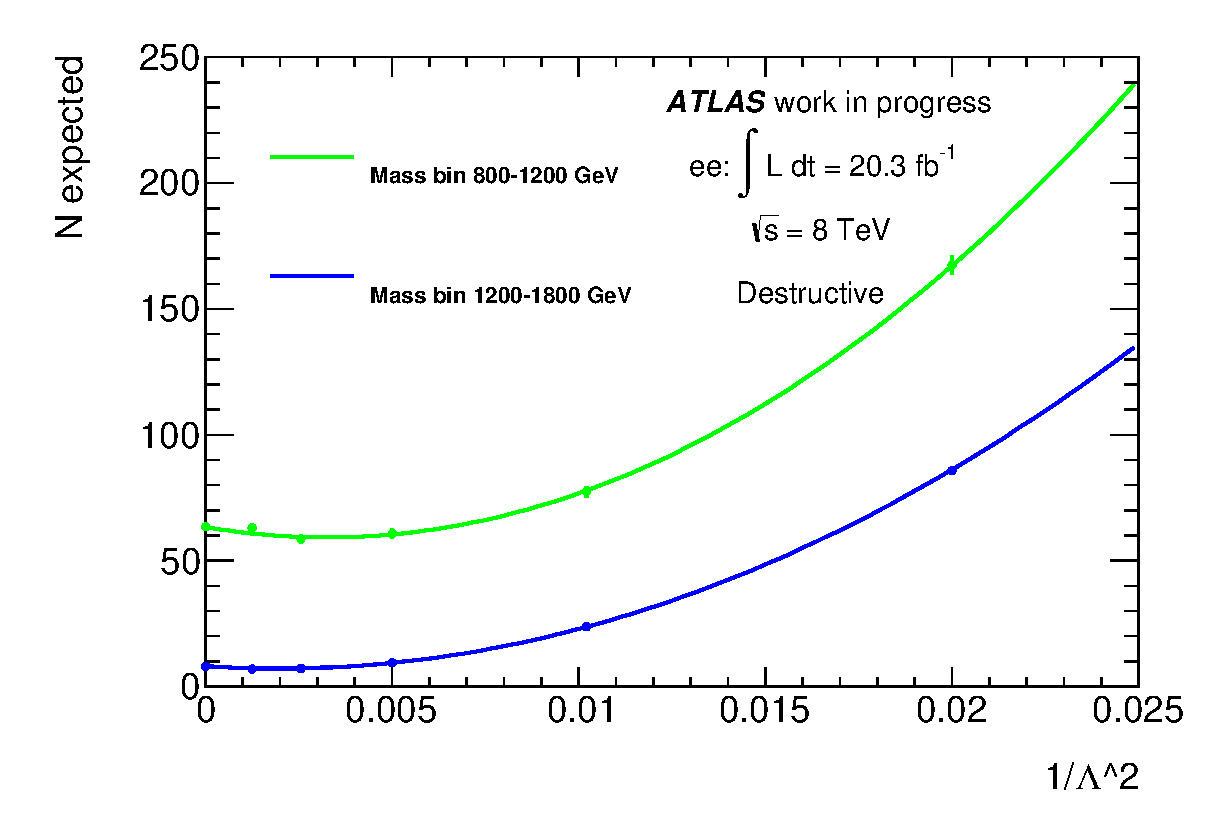
\includegraphics[width=0.49\linewidth]{images/parametrisations/NexpFits_plus_elec_midmass.eps} \\
	    	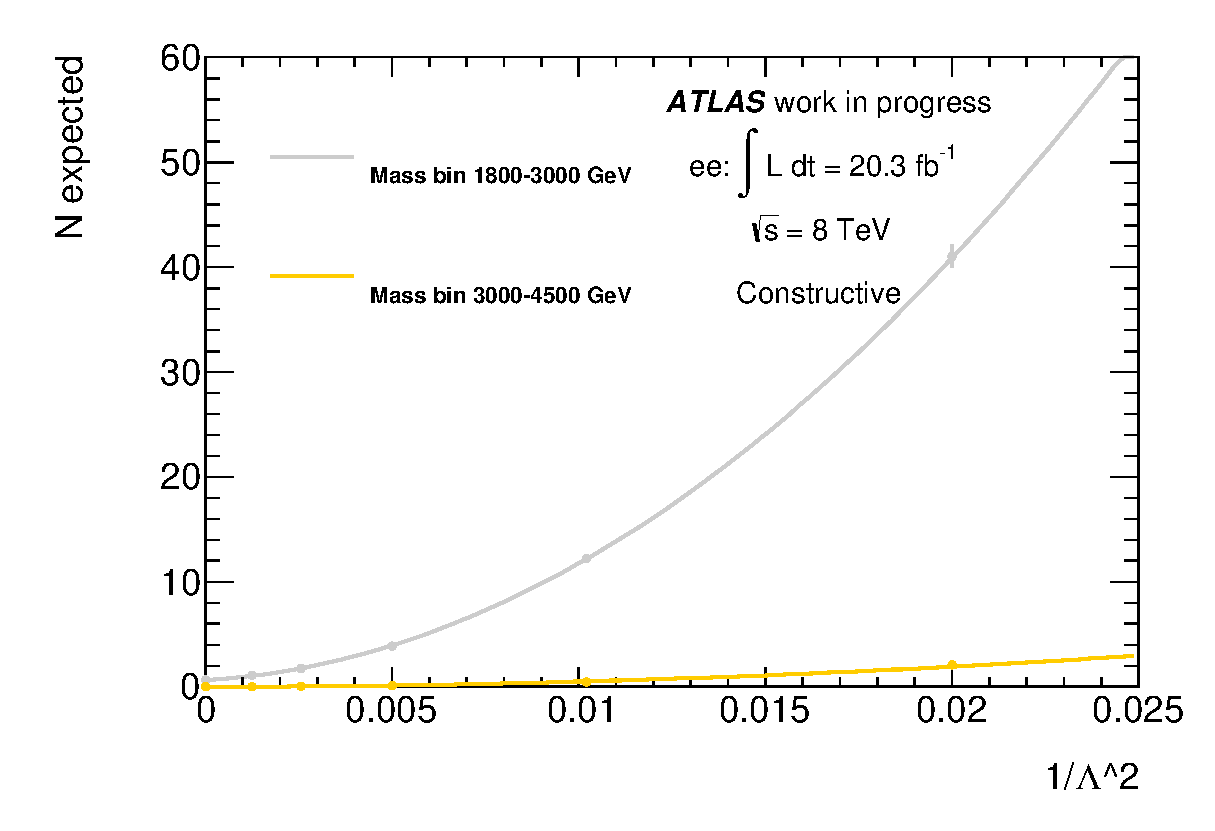
\includegraphics[width=0.49\linewidth]{images/parametrisations/NexpFits_minus_elec_himass.eps}
	    	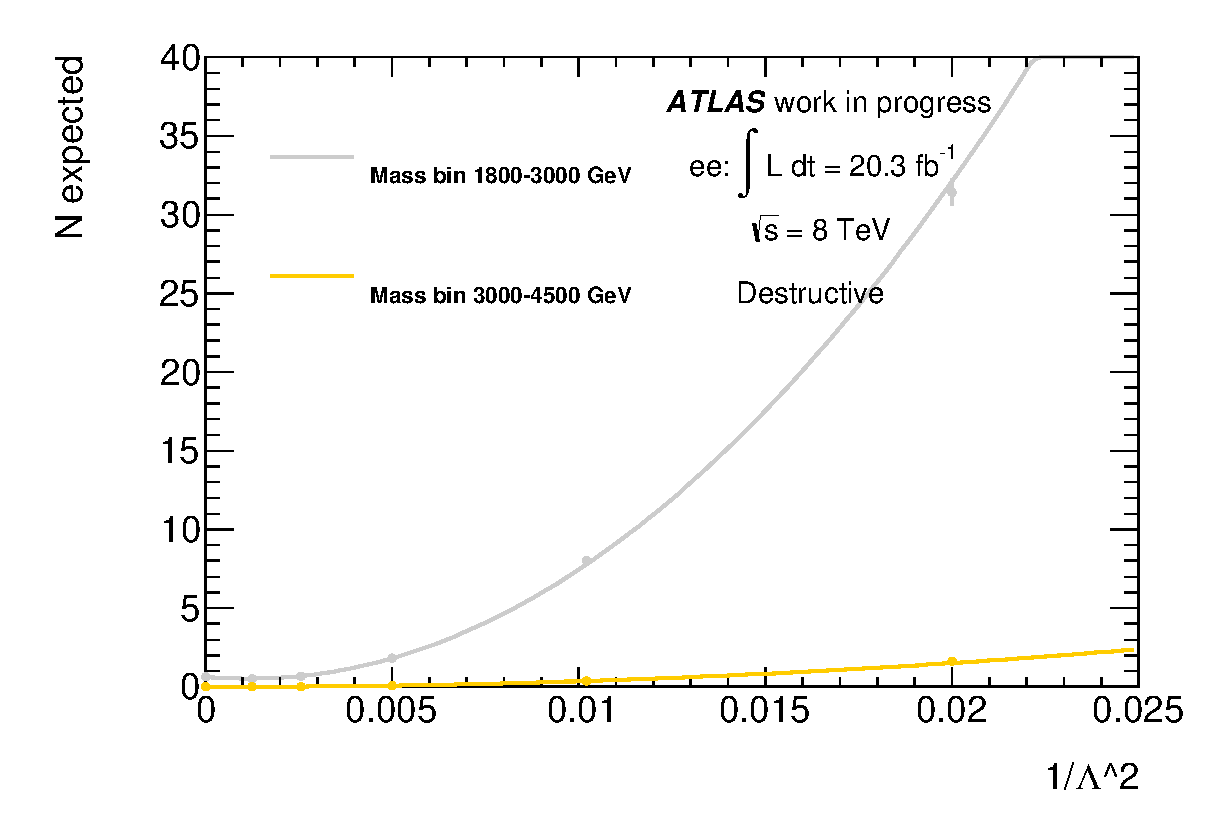
\includegraphics[width=0.49\linewidth]{images/parametrisations/NexpFits_plus_elec_himass.eps} \\
	    \end{center}
	   \caption{Parametrisations of the CI signal for number of expected events as a function of $\Lambda$ according to equation \ref{eq:CIparm} and for each CI mass bin.}
	   \label{fig:CIparm}
	\end{figure}

	% \begin{figure}[h]
	%     \begin{center}
	%     	%\includegraphics[scale=0.6]{images/}
	%     \end{center}
	%    \caption{Parametrisations of the ADD signal for number of expected events as a function of M$_{s}$ according to equation \ref{eq:ADDparm} for the ADD search bin.}
	%    \label{fig:ADDparm}
	% \end{figure}


\section{Results}

	Following are full results of the event selection for observed data, predicted background and some example signal models. Figures \ref{fig:invMass_main} and \ref{fig:cosTS_main} show the distributions of the two main search variables dielectron invariant mass and $\cos{\theta^{*}}$. A comparison between data and background is given with the expected shapes of some signal models shown for comparison. Ratio's are also shown between data and background along with a band showing the size of the total systematic uncertainty as described in section \ref{sec:sys}. Figure \ref{fig:AFB_main} then shows forward backward asymmetry ($A_{FB}$) defined in equation \ref{eq:AFB}. Statistical errors on the data points are calculated using the function $\Delta A_{FB} = \sqrt{(1-A_{FB}^{2})/N}$ where $N$ is the number of events in both the forward and backwards regions. The ratio shown in figure \ref{fig:AFB_main} is the difference between data and background $A_{FB}$ values, $\Delta$, divided by the total systematic uncertainty found in that bin, $\sigma$. It can be seen that data favours the angular dependence of the SM prediction or the CI LL formalism with no divergence similar to the CI LR formalism. 
	In figure \ref{fig:control_main} control plots are seen showing electron $p_{T}$, $\eta$ and $\phi$. More results and control plots can be found in appendix \ref{ap:contol}. 
	Lastly tables \ref{tab:CI_results0}, \ref{tab:CI_results1}, \ref{tab:CI_results2} and \ref{tab:CI_results3} show the full extracted results acceding through the search bins. Each invariant mass bin is shown as well as the forward and backwards regions within each bin where forward refers to events with $\cos{\theta^{*}}$ greater than 0 and backwards events with $\cos{\theta^{*}}$ less than 0. The expected number of events is given for each of the background as well as a selection of CI signal formalisms and the data observed. Table \ref{tab:ADD_results} shows the results for the single ADD search search bin the same as the CI tables. The reason a single bin is used is discussed in chapter \ref{ch:stat}.

	It can be seen from these results that no significant difference is seen between data observed and the background predicted. A slight discrepancy is seen between data and background in the 1200 - 1800 GeV invariant mass bin. The background predicts 10.8 events with a total systematic error of 1.6 events while only 7 events are observed in data. As seen later this doesn't signify a significant difference but has an effect on the limits set in chapter \ref{ch:stat}. 



	\begin{figure}[h]
	    \begin{center}
	    	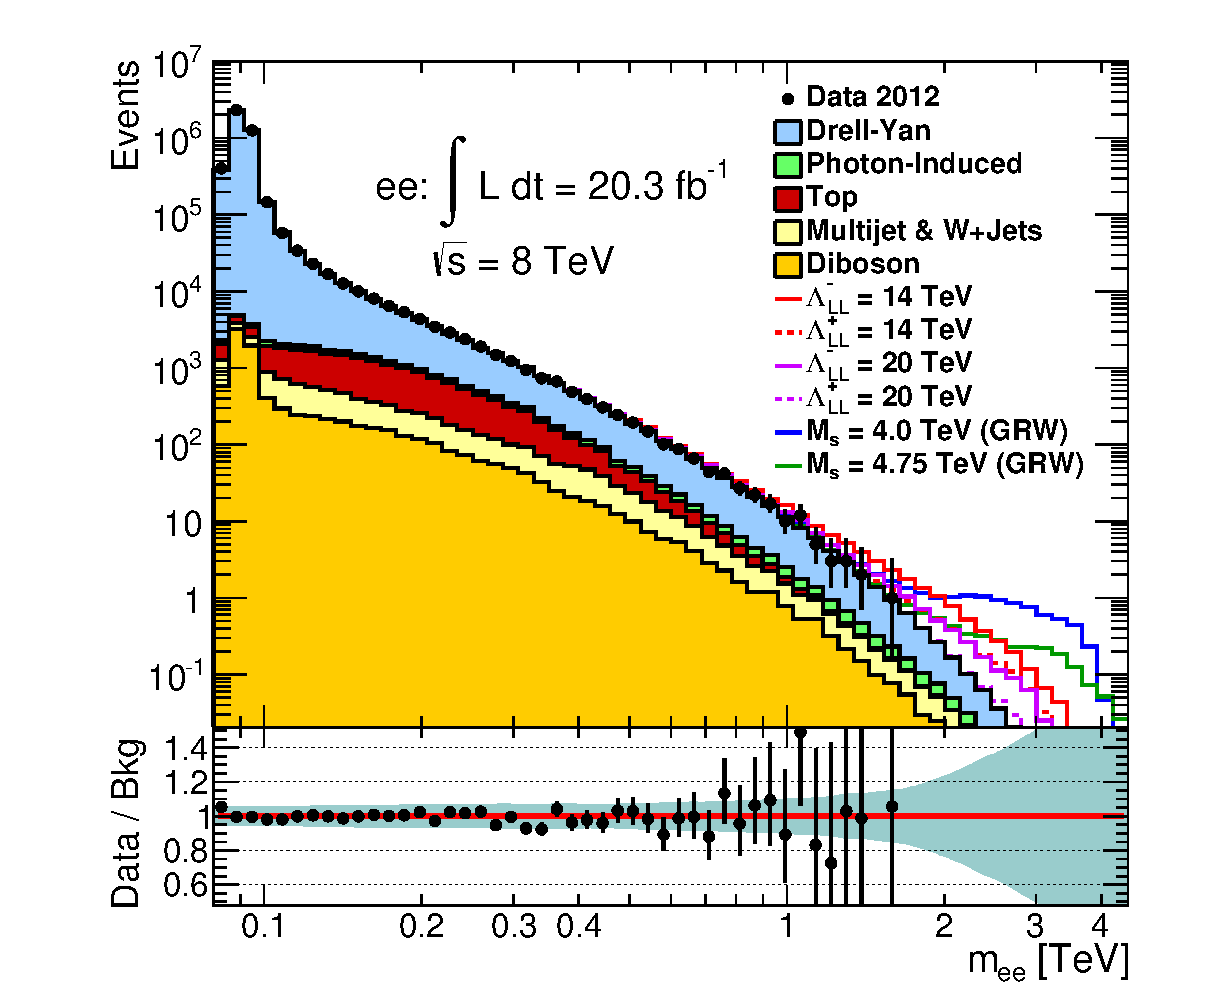
\includegraphics[width=0.8\linewidth]{images/invmass_main.eps}
	    \end{center}
	   \caption{Dielectron invariant mass comparison between data and MC with possible signal overlays of CI and ADD. Ratio between data and background included with band showing size of total background systematic. The distribution has bin width constant in $\log(M_{ee})$.}
	   \label{fig:invMass_main}
	\end{figure}

	\begin{figure}[h]
	    \begin{center}
	    	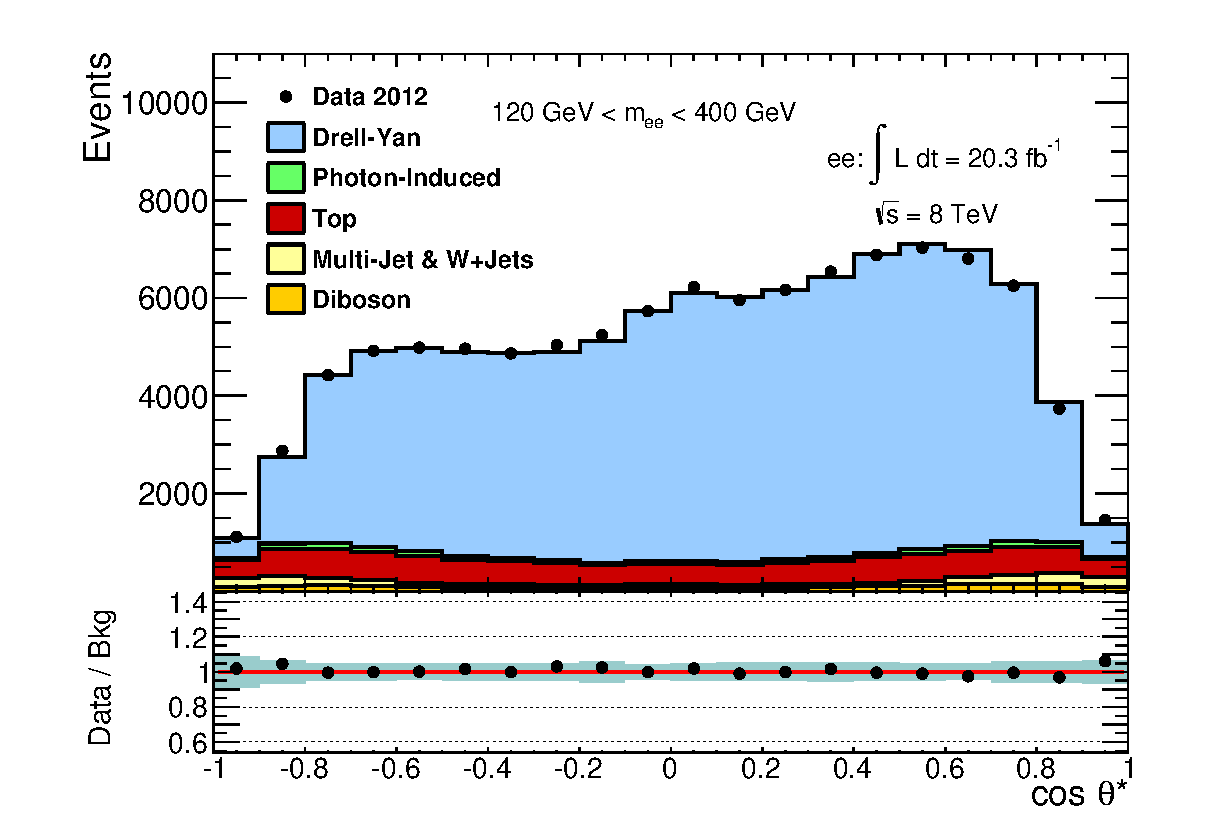
\includegraphics[width=0.9\linewidth]{images/CosThetaStar_Control_main.eps} \\
	    	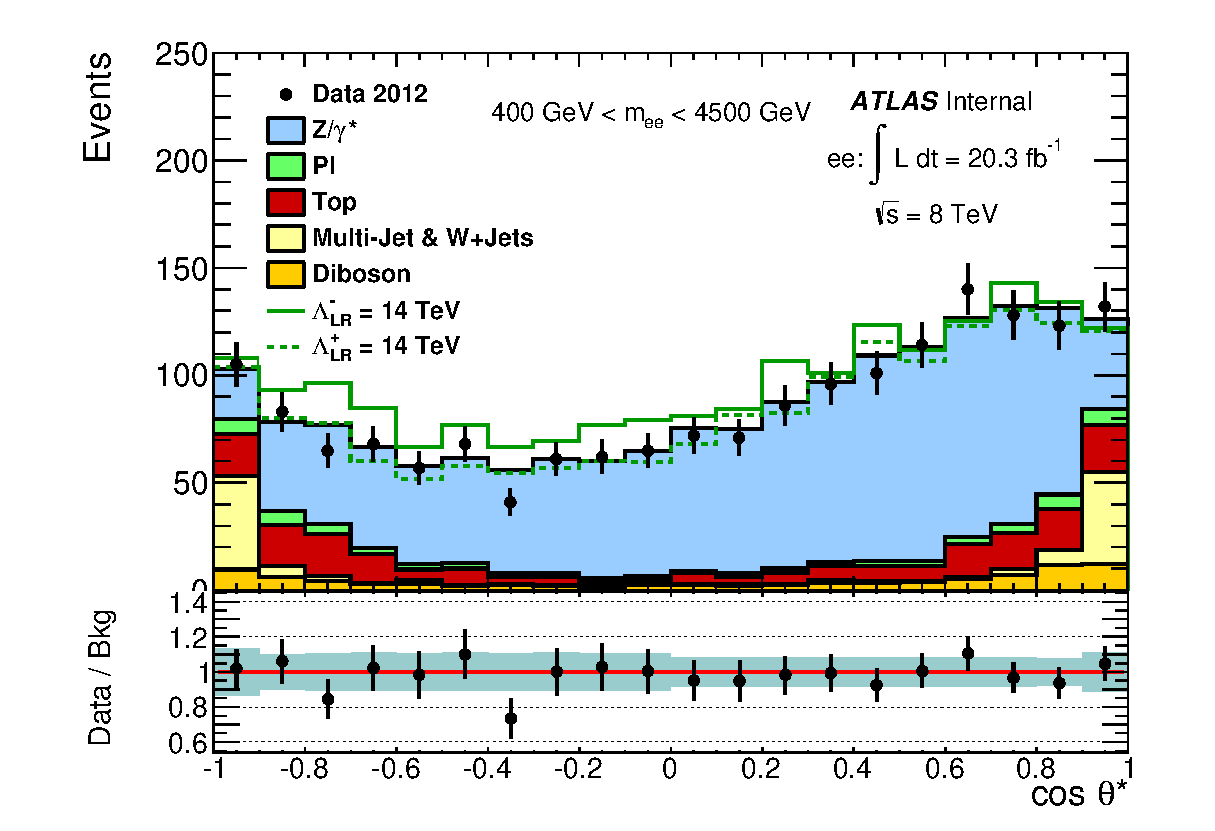
\includegraphics[width=0.9\linewidth]{images/CosThetaStar_Signal_main.eps}
	    \end{center}
	   \caption{$\cos{\theta^{*}}$ comparison between data and MC in control and signal regions with possible signal overlay of the CI LR formalism. Ratio between data and background included with band showing size of total background systematic. $\cos{\theta^{*}}$ plots for each mass bin are found in appendix \ref{ap:contol}.}
	   \label{fig:cosTS_main}
	\end{figure}

	\begin{figure}[h]
	    \begin{center}
	    	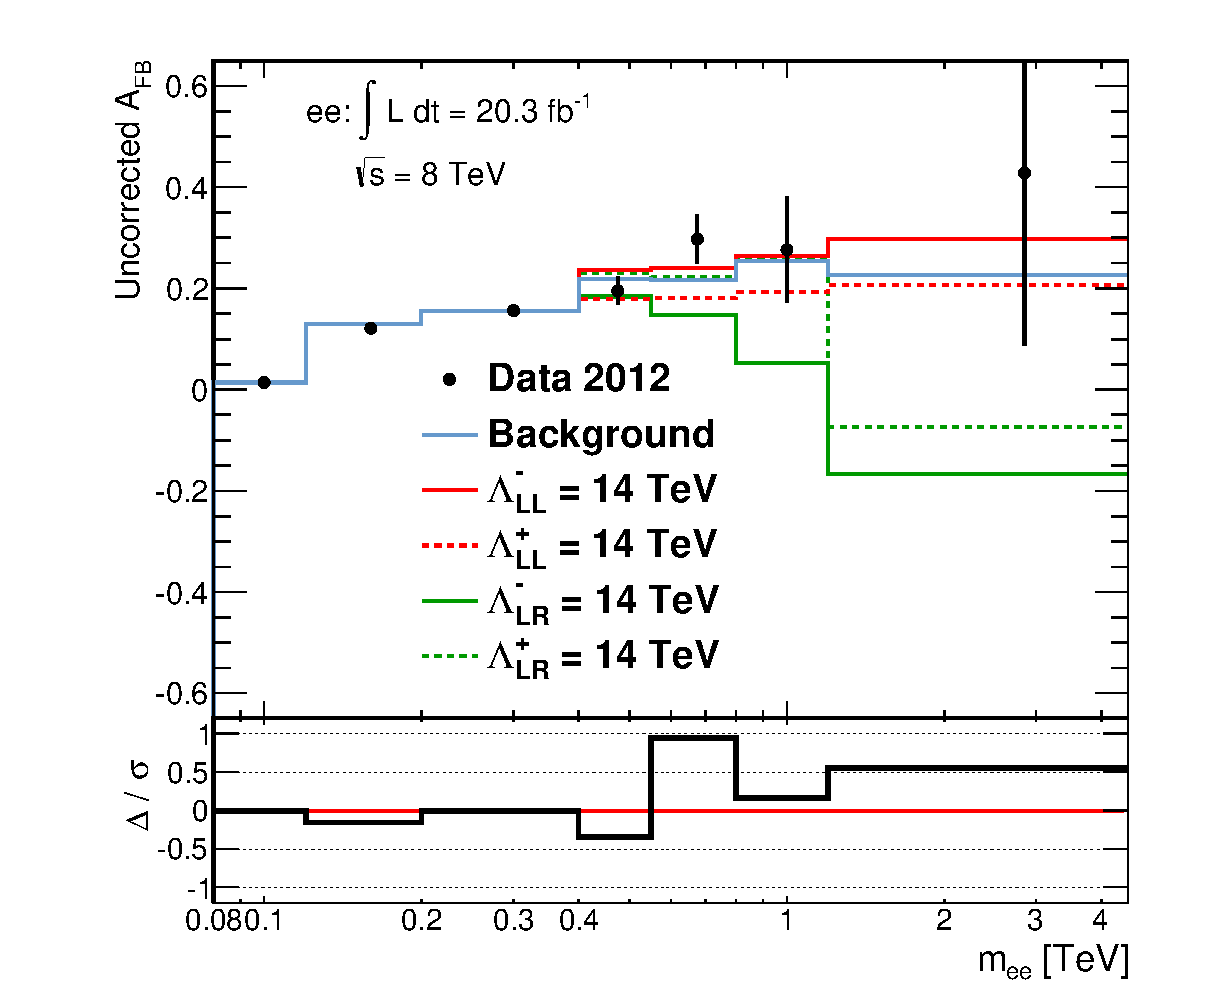
\includegraphics[width=0.8\linewidth]{images/A_fb_main.eps}
	    \end{center}
	   \caption{A$_{FB}$ comparison between data and MC with possible signal overlay of CI. Ratio shows the difference between data and background prediction divided by total background systematic.}
	   \label{fig:AFB_main}
	\end{figure}



	\begin{figure}[h]
	    \begin{center}
	    	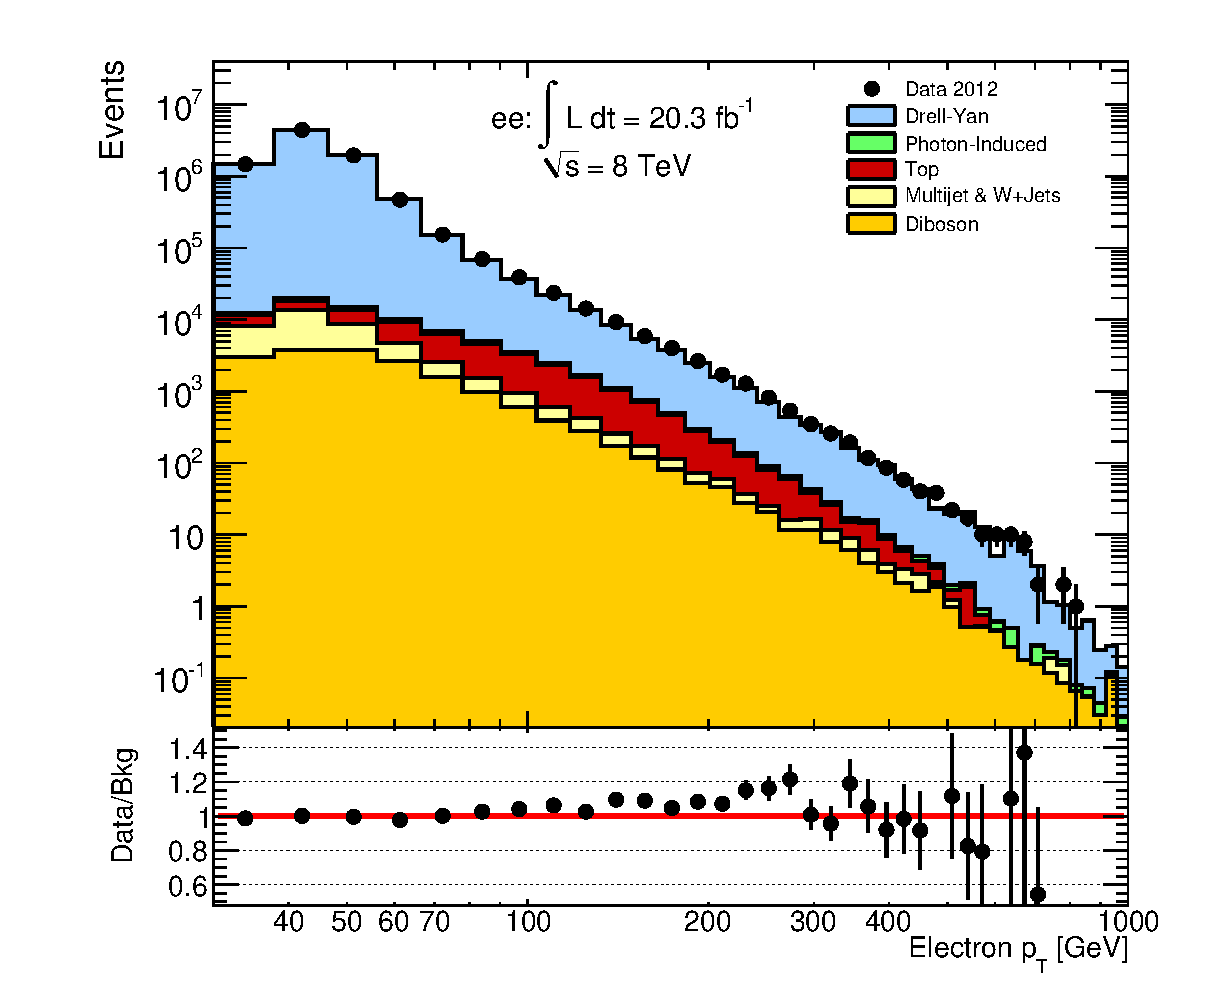
\includegraphics[width=0.8\linewidth]{images/pT_main.eps} \\
	    	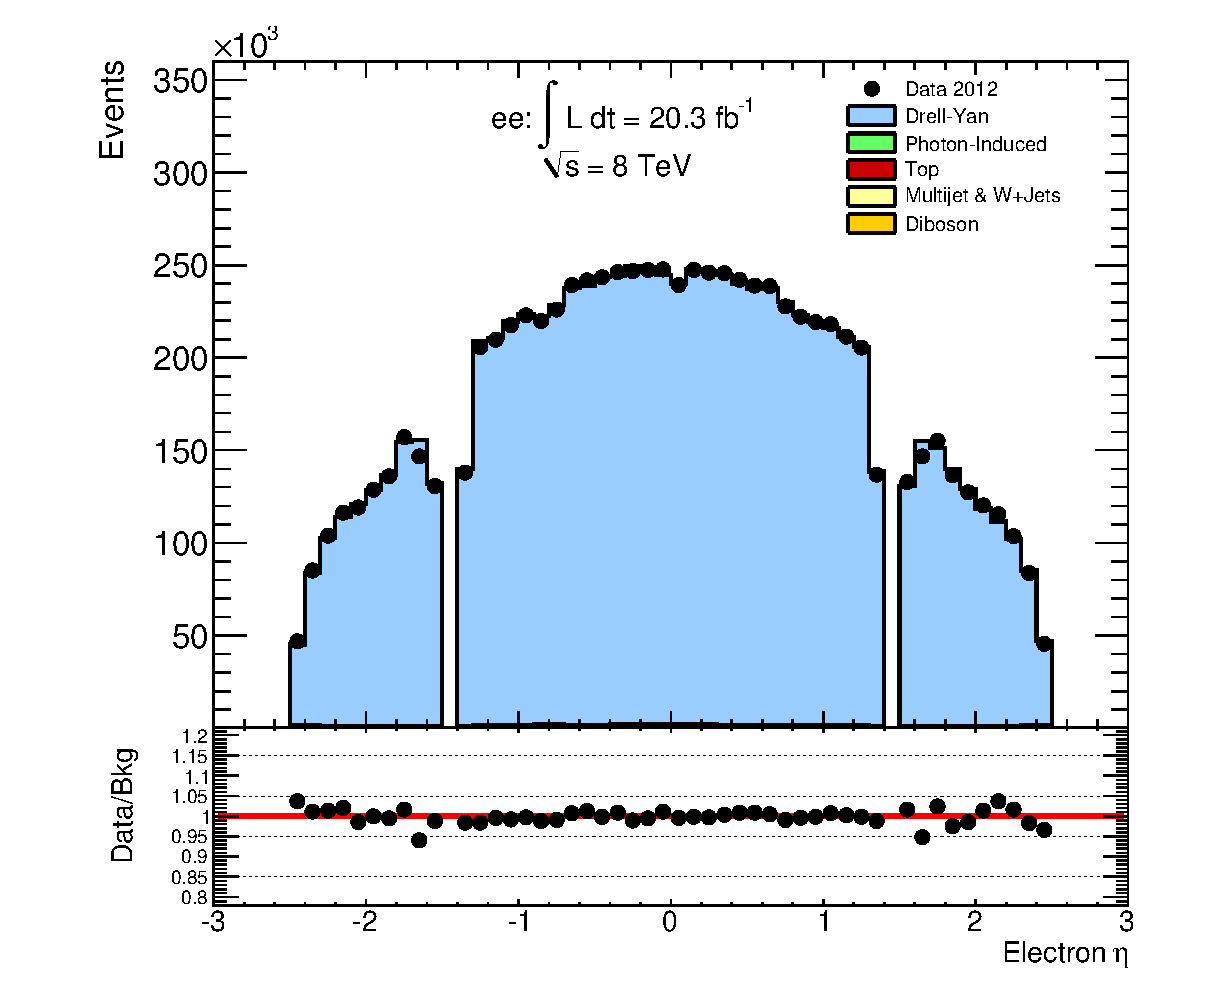
\includegraphics[width=0.49\linewidth]{images/eta_main.eps}
	    	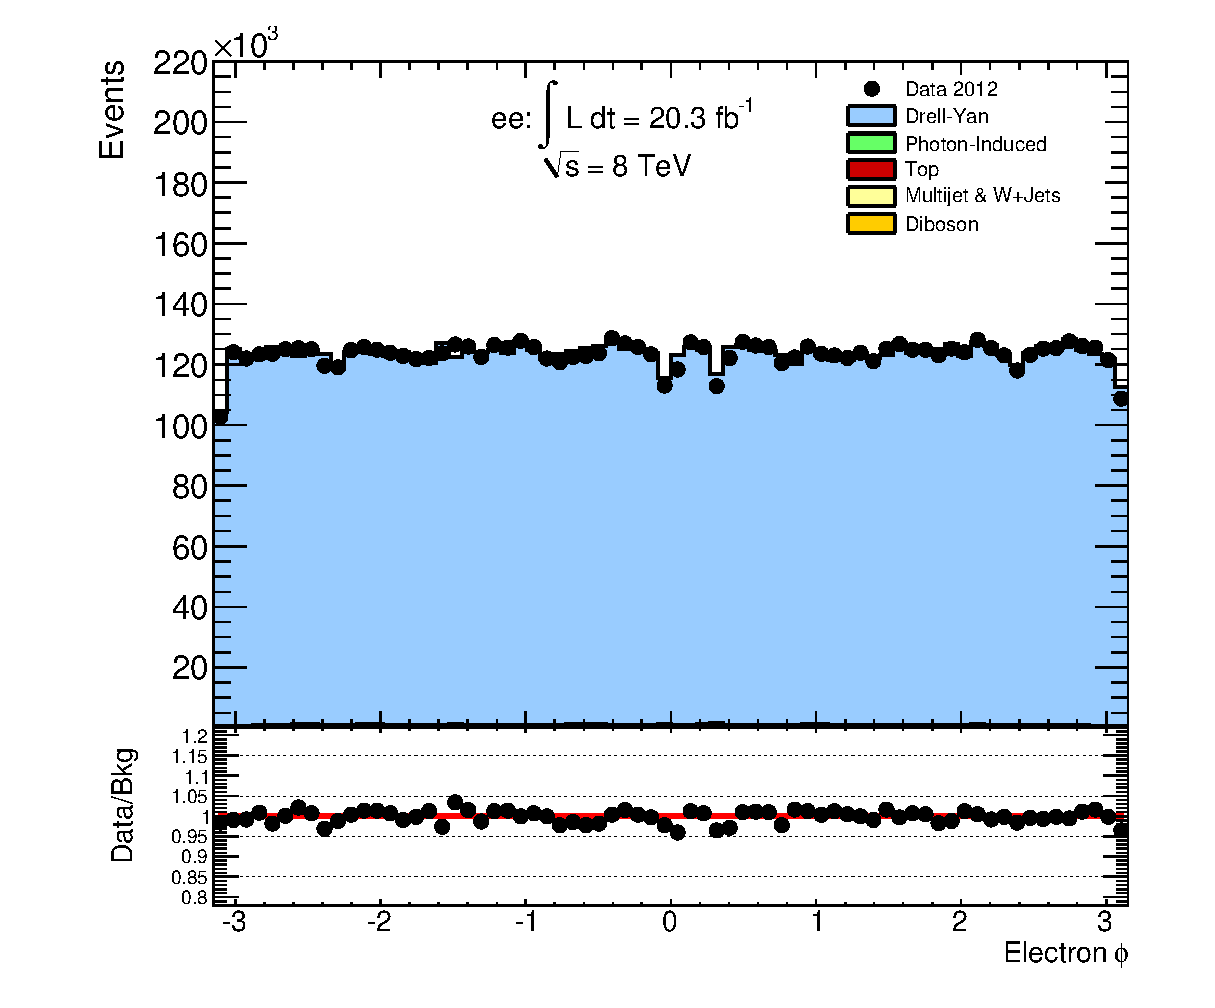
\includegraphics[width=0.49\linewidth]{images/phi_main.eps}
	    \end{center}
	   \caption{Control plots of $p_{T}$, $\eta$ and $\phi$ distributions of selected electrons.}
	   \label{fig:control_main}
	\end{figure}


	\begin {table}[h]
		\scriptsize  
		\begin{center}
		\begin{tabular}{  l | c c c | c c c  } 
			\hline
			\hline
			\multirow{3}{*}{Process} 	& \multicolumn{6}{c}{$m_{ee}$ [GeV]} \\
										& \multicolumn{3}{c}{120 - 200} & \multicolumn{3}{c}{200 - 400} \\
										\cline{2-7}
										& All & Forward & Backward & All & Forward & Backward \\
			\hline
			Drell-Yan & 72000 $\pm$ 5000 & 41500 $\pm$ 2600 & 31000 $\pm$ 2200 & 13100 $\pm$ 900 & 7900 $\pm$ 500 & 5200 $\pm$ 400 \\
			Top & 6900 $\pm$ 400 & 3480 $\pm$ 210 & 3410 $\pm$ 210 & 2840 $\pm$ 170 & 1400 $\pm$ 90 & 1440 $\pm$ 90 \\
			Multijets \& W+Jets & 1650 $\pm$ 330 & 900 $\pm$ 180 & 780 $\pm$ 160 & 670 $\pm$ 130 & 330 $\pm$ 70 & 340 $\pm$ 70 \\
			Diboson & 1330 $\pm$ 70 & 710 $\pm$ 40 & 619 $\pm$ 33 & 583 $\pm$ 31 & 331 $\pm$ 19 & 252 $\pm$ 15 \\
			Photon-Induced & 1200 $\pm$ 1200 & 600 $\pm$ 600 & 600 $\pm$ 600 & 400 $\pm$ 400 & 230 $\pm$ 230 & 220 $\pm$ 220 \\
			\hline
			Total SM & 84000 $\pm$ 5000 & 47200 $\pm$ 2800 & 36400 $\pm$ 2500 & 17600 $\pm$ 1200 & 10200 $\pm$ 600 & 7400 $\pm$ 500 \\
			\hline
			Data & 83824 & 46910 & 36914 & 17525 & 10107 & 7418 \\
			\hline
			\hline
		\end{tabular}
	  	\caption{Comparison of background prediction to data. Binning covering the control region. Total systematic error is included on each number. See section \ref{sec:sys} for details of systematics.}
	  	\label{tab:CI_results0}
	  	\end{center}
	\end {table}

	\begin {table}[h]
		\scriptsize  
		\begin{center}
		\begin{tabular}{  l | c c c | c c c  } 
			\hline
			\hline
			\multirow{3}{*}{Process} 	& \multicolumn{6}{c}{$m_{ee}$ [GeV]} \\
										& \multicolumn{3}{c}{400 - 550} & \multicolumn{3}{c}{550 - 800} \\
										\cline{2-7}
										& All & Forward & Backward & All & Forward & Backward \\
			\hline
			Drell-Yan & 910 $\pm$ 70 & 580 $\pm$ 40 & 333 $\pm$ 32 & 302 $\pm$ 25 & 193 $\pm$ 13 & 109 $\pm$ 12 \\
			Top & 153 $\pm$ 13 & 87 $\pm$ 8 & 72 $\pm$ 7 & 35.2 $\pm$ 2.7 & 18.2 $\pm$ 1.6 & 17.5 $\pm$ 1.6 \\
			Multijets \& W+Jets & 88 $\pm$ 18 & 43 $\pm$ 9 & 45 $\pm$ 9 & 27 $\pm$ 6 & 13.0 $\pm$ 3.0 & 13.0 $\pm$ 3.1 \\
			Diboson & 62.2 $\pm$ 3.5 & 36.0 $\pm$ 2.2 & 26.2 $\pm$ 1.7 & 22.3 $\pm$ 1.3 & 13.8 $\pm$ 0.9 & 8.5 $\pm$ 0.7 \\
			Photon-Induced & 40 $\pm$ 40 & 22 $\pm$ 22 & 22 $\pm$ 22 & 17 $\pm$ 17 & 8 $\pm$ 8 & 8 $\pm$ 8 \\
			\hline
			Total SM & 1260 $\pm$ 100 & 770 $\pm$ 50 & 500 $\pm$ 50 & 404 $\pm$ 35 & 247 $\pm$ 18 & 156 $\pm$ 17 \\
			\hline
			Data & 1262 & 754 & 508 & 388 & 251 & 137 \\
			\hline
			SM+CI($\Lambda^{-14}_{LL}$) & 1310 $\pm$ 110 & 810 $\pm$ 60 & 510 $\pm$ 50 & 440 $\pm$ 40 & 276 $\pm$ 22 & 167 $\pm$ 18 \\
			SM+CI($\Lambda^{-20}_{LL}$) & 1290 $\pm$ 110 & 780 $\pm$ 60 & 510 $\pm$ 50 & 430 $\pm$ 40 & 271 $\pm$ 22 & 157 $\pm$ 18 \\
			SM+CI($\Lambda^{-14}_{LR}$) & 1340 $\pm$ 110 & 790 $\pm$ 60 & 550 $\pm$ 50 & 460 $\pm$ 40 & 266 $\pm$ 22 & 195 $\pm$ 19 \\
			SM+CI($\Lambda^{-20}_{LR}$) & 1290 $\pm$ 110 & 780 $\pm$ 60 & 510 $\pm$ 50 & 420 $\pm$ 40 & 249 $\pm$ 21 & 174 $\pm$ 19 \\
			SM+CI($\Lambda^{-14}_{RR}$) & 1310 $\pm$ 110 & 810 $\pm$ 60 & 510 $\pm$ 50 & 440 $\pm$ 40 & 276 $\pm$ 22 & 167 $\pm$ 18 \\
			SM+CI($\Lambda^{-20}_{RR}$) & 1290 $\pm$ 110 & 780 $\pm$ 60 & 510 $\pm$ 50 & 430 $\pm$ 40 & 271 $\pm$ 22 & 157 $\pm$ 18 \\
			\hline
			SM+CI($\Lambda^{+14}_{LL}$) & 1230 $\pm$ 110 & 730 $\pm$ 60 & 510 $\pm$ 50 & 380 $\pm$ 40 & 227 $\pm$ 21 & 155 $\pm$ 18 \\
			SM+CI($\Lambda^{+20}_{LL}$) & 1230 $\pm$ 110 & 740 $\pm$ 60 & 490 $\pm$ 50 & 390 $\pm$ 40 & 234 $\pm$ 21 & 156 $\pm$ 18 \\
			SM+CI($\Lambda^{+14}_{LR}$) & 1200 $\pm$ 110 & 740 $\pm$ 60 & 470 $\pm$ 50 & 400 $\pm$ 40 & 247 $\pm$ 21 & 154 $\pm$ 18 \\
			SM+CI($\Lambda^{+20}_{LR}$) & 1210 $\pm$ 110 & 740 $\pm$ 60 & 470 $\pm$ 50 & 390 $\pm$ 40 & 238 $\pm$ 21 & 150 $\pm$ 18 \\
			SM+CI($\Lambda^{+14}_{RR}$) & 1230 $\pm$ 110 & 730 $\pm$ 60 & 510 $\pm$ 50 & 380 $\pm$ 40 & 227 $\pm$ 21 & 155 $\pm$ 18 \\
			SM+CI($\Lambda^{+20}_{RR}$) & 1230 $\pm$ 110 & 740 $\pm$ 60 & 490 $\pm$ 50 & 390 $\pm$ 40 & 234 $\pm$ 21 & 156 $\pm$ 18 \\
			\hline
			\hline
		\end{tabular}
	  	\caption{Comparison of background prediction to data with prediction of several CI signal models. Signal models are refereed to showing constructive or destructive interference (-/+ in superscript), $\Lambda$ value (numberin superscript) and formalism (letters in subscript). Binning used is the same as used for statistical analysis of CI model with the two lowest mass regions shown here. Total systematic error is included on each number. See section \ref{sec:sys} for details of systematics.}
	  	\label{tab:CI_results1}
	  	\end{center}
	\end {table}

	\begin {table}[h]
		\scriptsize 
		\begin{center}
		\begin{tabular}{  l | c c c | c c c  }	
			\hline
			\hline
			\multirow{3}{*}{Process} 	& \multicolumn{6}{c}{$m_{ee}$ [GeV]} \\
										& \multicolumn{3}{c}{800 - 1200} & \multicolumn{3}{c}{1200 - 1800} \\
										\cline{2-7}
										& All & Forward & Backward & All & Forward & Backward \\
			\hline
			Drell-Yan & 63 $\pm$ 6 & 41.4 $\pm$ 3.4 & 22.1 $\pm$ 2.9 & 8.2 $\pm$ 1.2 & 5.3 $\pm$ 0.6 & 2.9 $\pm$ 0.6 \\
			Top & 3.06 $\pm$ 0.18 & 1.58 $\pm$ 0.10 & 1.45 $\pm$ 0.09 & 0.140 $\pm$ 0.008 & 0.073 $\pm$ 0.004 & 0.065 $\pm$ 0.004 \\
			Multijets \& W+Jets & 5.8 $\pm$ 1.5 & 2.6 $\pm$ 0.9 & 2.5 $\pm$ 0.8 & 0.87 $\pm$ 0.32 & 0.35 $\pm$ 0.16 & 0.32 $\pm$ 0.24 \\
			Diboson & 5.4 $\pm$ 0.4 & 3.41 $\pm$ 0.28 & 2.02 $\pm$ 0.17 & 0.83 $\pm$ 0.05 & 0.542 $\pm$ 0.035 & 0.287 $\pm$ 0.016 \\
			Photon-Induced & 4 $\pm$ 4 & 2.2 $\pm$ 2.2 & 2.1 $\pm$ 2.1 & 0.7 $\pm$ 0.7 & 0.34 $\pm$ 0.34 & 0.4 $\pm$ 0.4 \\
			\hline
			Total SM & 82 $\pm$ 9 & 51 $\pm$ 5 & 30 $\pm$ 4 & 10.8 $\pm$ 1.6 & 6.6 $\pm$ 0.7 & 4.0 $\pm$ 0.8 \\
			\hline
			Data & 84 & 53 & 31 & 7 & 5 & 2 \\
			\hline
			SM+CI($\Lambda^{-14}_{LL}$) & 108 $\pm$ 10 & 68 $\pm$ 6 & 39 $\pm$ 5 & 20.9 $\pm$ 1.9 & 13.5 $\pm$ 1.0 & 7.2 $\pm$ 0.9 \\
			SM+CI($\Lambda^{-20}_{LL}$) & 90 $\pm$ 10 & 58 $\pm$ 5 & 32 $\pm$ 4 & 14.4 $\pm$ 1.7 & 9.2 $\pm$ 0.9 & 5.0 $\pm$ 0.8 \\
			SM+CI($\Lambda^{-14}_{LR}$) & 118 $\pm$ 10 & 62 $\pm$ 6 & 56 $\pm$ 5 & 26.3 $\pm$ 2.1 & 11.3 $\pm$ 1.0 & 14.8 $\pm$ 1.1 \\
			SM+CI($\Lambda^{-20}_{LR}$) & 98 $\pm$ 10 & 57 $\pm$ 5 & 41 $\pm$ 5 & 15.7 $\pm$ 1.7 & 8.3 $\pm$ 0.9 & 7.2 $\pm$ 0.9 \\
			SM+CI($\Lambda^{-14}_{RR}$) & 108 $\pm$ 10 & 68 $\pm$ 6 & 40 $\pm$ 5 & 20.8 $\pm$ 1.9 & 13.6 $\pm$ 1.0 & 6.9 $\pm$ 0.9 \\
			SM+CI($\Lambda^{-20}_{RR}$) & 91 $\pm$ 10 & 58 $\pm$ 5 & 32 $\pm$ 4 & 14.3 $\pm$ 1.7 & 9.1 $\pm$ 0.9 & 5.0 $\pm$ 0.8 \\
			\hline
			SM+CI($\Lambda^{+14}_{LL}$) & 79 $\pm$ 9 & 47 $\pm$ 5 & 32 $\pm$ 4 & 12.2 $\pm$ 1.7 & 7.3 $\pm$ 0.8 & 4.7 $\pm$ 0.8 \\
			SM+CI($\Lambda^{+20}_{LL}$) & 77 $\pm$ 9 & 48 $\pm$ 5 & 29 $\pm$ 4 & 10.0 $\pm$ 1.6 & 6.1 $\pm$ 0.8 & 3.7 $\pm$ 0.8 \\
			SM+CI($\Lambda^{+14}_{LR}$) & 88 $\pm$ 10 & 55 $\pm$ 5 & 32 $\pm$ 4 & 18.9 $\pm$ 1.8 & 9.2 $\pm$ 0.9 & 9.5 $\pm$ 0.9 \\
			SM+CI($\Lambda^{+20}_{LR}$) & 81 $\pm$ 9 & 52 $\pm$ 5 & 29 $\pm$ 4 & 11.5 $\pm$ 1.6 & 6.8 $\pm$ 0.8 & 4.5 $\pm$ 0.8 \\
			SM+CI($\Lambda^{+14}_{RR}$) & 79 $\pm$ 9 & 47 $\pm$ 5 & 32 $\pm$ 4 & 12.1 $\pm$ 1.7 & 7.3 $\pm$ 0.8 & 4.6 $\pm$ 0.8 \\
			SM+CI($\Lambda^{+20}_{RR}$) & 77 $\pm$ 9 & 48 $\pm$ 5 & 29 $\pm$ 4 & 10.2 $\pm$ 1.6 & 6.3 $\pm$ 0.8 & 3.8 $\pm$ 0.8 \\
			\hline
			\hline
		\end{tabular}
	  	\caption{Comparison of background prediction to data with prediction of several CI signal models. Signal models are refereed to showing constructive or destructive interference (-/+ in superscript), $\Lambda$ value (numberin superscript) and formalism (letters in subscript). Binning used is the same as used for statistical analysis of CI model with the two mid mass regions shown here. Total systematic error is included on each number. See section \ref{sec:sys} for details of systematics.}
	  	\label{tab:CI_results2}
	  	\end{center}
	\end {table}



	\begin {table}[h]
		\scriptsize 
		\begin{center}
		\begin{tabular}{  l | c c c | c c c  }
			\hline
			\hline
			\multirow{3}{*}{Process} 	& \multicolumn{6}{c}{$m_{ee}$ [GeV]} \\
										& \multicolumn{3}{c}{1800 - 3000} & \multicolumn{3}{c}{3000 - 4500} \\
										\cline{2-7}
										& All & Forward & Backward & All & Forward & Backward \\
			\hline
			Drell-Yan & 0.64 $\pm$ 0.17 & 0.41 $\pm$ 0.09 & 0.23 $\pm$ 0.08 & 0.006 $\pm$ 0.004 & 0.0039 $\pm$ 0.0021 & 0.0022 $\pm$ 0.0018 \\
			Top & $<$ 0.004   & $<$ 0.002   & $<$ 0.002   & $<$ 0.001   & $<$ 0.001   & $<$ 0.001   \\
			Multijets \& W+Jets & 0.11 $\pm$ 0.04 & 0.040 $\pm$ 0.020 & 0.033 $\pm$ 0.027 & 0.0058 $\pm$ 0.0012 & $<$ 0.002   & $<$ 0.001   \\
			Diboson & 0.075 $\pm$ 0.006 & 0.053 $\pm$ 0.004 & 0.0224 $\pm$ 0.0026 & $<$ 0.001   & $<$ 0.001   & $<$ 0.001   \\
			Photon-Induced & 0.08 $\pm$ 0.08 & 0.04 $\pm$ 0.04 & 0.04 $\pm$ 0.04 & 0.0016 $\pm$ 0.0016 & $<$ 0.002   & $<$ 0.002   \\
			\hline
			Total SM & 0.91 $\pm$ 0.21 & 0.55 $\pm$ 0.10 & 0.33 $\pm$ 0.10 & 0.014 $\pm$ 0.005 & 0.0065 $\pm$ 0.0026 & 0.0042 $\pm$ 0.0022 \\
			\hline
			Data & 0 & 0 & 0 & 0 & 0 & 0 \\
			\hline
			SM+CI($\Lambda^{-14}_{LL}$) & 4.2 $\pm$ 0.4 & 2.75 $\pm$ 0.23 & 1.38 $\pm$ 0.15 & 0.141 $\pm$ 0.028 & 0.080 $\pm$ 0.020 & 0.058 $\pm$ 0.016 \\
			SM+CI($\Lambda^{-20}_{LL}$) & 2.01 $\pm$ 0.25 & 1.26 $\pm$ 0.14 & 0.72 $\pm$ 0.12 & 0.045 $\pm$ 0.012 & 0.021 $\pm$ 0.007 & 0.022 $\pm$ 0.007 \\
			SM+CI($\Lambda^{-14}_{LR}$) & 6.0 $\pm$ 0.5 & 2.31 $\pm$ 0.21 & 3.69 $\pm$ 0.30 & 0.28 $\pm$ 0.05 & 0.127 $\pm$ 0.030 & 0.146 $\pm$ 0.032 \\
			SM+CI($\Lambda^{-20}_{LR}$) & 2.58 $\pm$ 0.28 & 1.01 $\pm$ 0.13 & 1.54 $\pm$ 0.16 & 0.078 $\pm$ 0.018 & 0.036 $\pm$ 0.011 & 0.039 $\pm$ 0.012 \\
			SM+CI($\Lambda^{-14}_{RR}$) & 3.78 $\pm$ 0.34 & 2.51 $\pm$ 0.22 & 1.23 $\pm$ 0.15 & 0.23 $\pm$ 0.04 & 0.155 $\pm$ 0.031 & 0.069 $\pm$ 0.018 \\
			SM+CI($\Lambda^{-20}_{RR}$) & 1.86 $\pm$ 0.24 & 1.11 $\pm$ 0.13 & 0.71 $\pm$ 0.12 & 0.072 $\pm$ 0.015 & 0.047 $\pm$ 0.011 & 0.022 $\pm$ 0.008 \\
			\hline
			SM+CI($\Lambda^{+14}_{LL}$) & 2.08 $\pm$ 0.25 & 1.30 $\pm$ 0.14 & 0.75 $\pm$ 0.12 & 0.075 $\pm$ 0.015 & 0.050 $\pm$ 0.012 & 0.023 $\pm$ 0.007 \\
			SM+CI($\Lambda^{+20}_{LL}$) & 0.95 $\pm$ 0.22 & 0.55 $\pm$ 0.11 & 0.36 $\pm$ 0.11 & 0.029 $\pm$ 0.008 & 0.019 $\pm$ 0.006 & 0.0073 $\pm$ 0.0034 \\
			SM+CI($\Lambda^{+14}_{LR}$) & 4.2 $\pm$ 0.4 & 1.60 $\pm$ 0.16 & 2.51 $\pm$ 0.22 & 0.191 $\pm$ 0.034 & 0.081 $\pm$ 0.020 & 0.107 $\pm$ 0.023 \\
			SM+CI($\Lambda^{+20}_{LR}$) & 1.65 $\pm$ 0.24 & 0.82 $\pm$ 0.12 & 0.79 $\pm$ 0.12 & 0.058 $\pm$ 0.013 & 0.017 $\pm$ 0.006 & 0.039 $\pm$ 0.010 \\
			SM+CI($\Lambda^{+14}_{RR}$) & 2.26 $\pm$ 0.26 & 1.44 $\pm$ 0.15 & 0.78 $\pm$ 0.12 & 0.098 $\pm$ 0.018 & 0.057 $\pm$ 0.012 & 0.038 $\pm$ 0.010 \\
			SM+CI($\Lambda^{+20}_{RR}$) & 1.06 $\pm$ 0.22 & 0.65 $\pm$ 0.11 & 0.37 $\pm$ 0.11 & 0.036 $\pm$ 0.009 & 0.028 $\pm$ 0.008 & 0.0044 $\pm$ 0.0029 \\
			\hline
	    	\hline
	  	\end{tabular}
	  	\caption{Comparison of background prediction to data with prediction of several CI signal models. Signal models are refereed to showing constructive or destructive interference (-/+ in superscript), $\Lambda$ value (numberin superscript) and formalism (letters in subscript). Binning used is the same as used for statistical analysis of CI model with the two high mass regions shown here. Total systematic error is included on each number. See section \ref{sec:sys} for details of systematics.}
	  	\label{tab:CI_results3}
	  	\end{center}
	\end {table}






	\begin {table}[h]
		\begin{center}
		\begin{tabular}{  l | c } 
			\hline
			\hline
			Process & 1900 $\le$ $m_{ee}$ $\le$ 4500 GeV \\
			\hline
			Drell-Yan & 0.435 $\pm$ 0.002 \\
			Top & 0.003$\pm$ 0.000 \\
			Multi-Jet & 0.062 $\pm$ 0.012 \\
			Diboson & 0.053 $\pm$ 0.004 \\
			Photon-Induced & 0.058 $\pm$ 0.001 \\
			\hline
			Total SM & 0.611 $\pm$ 0.129 \\
			\hline
			Data & 0 \\ 
			\hline
			SM+ADD ($M_{S}$ = 3.50~TeV)& 21.637 $\pm$  2.144 \\
			SM+ADD ($M_{S}$ = 3.75~TeV)& 13.171 $\pm$  1.295 \\
			SM+ADD ($M_{S}$ = 4.00~TeV)& 8.436 $\pm$  0.821 \\
			SM+ADD ($M_{S}$ = 4.75~TeV)& 2.952 $\pm$  0.282 \\
	    	\hline
	    	\hline
	  	\end{tabular}
	  	\caption{Comparison of background prediction to data with prediction of several ADD signal models. One bin used the same in the statistical analysis of ADD. Total systematic error is included on each number. See section \ref{sec:sys} for details of systematics.}
	  	\label{tab:ADD_results}
	  	\end{center}
	\end {table}










\newpage
\chapter{Statistical Analysis}
    \label{ch:stat}

	The statistical analysis of results is done via a Bayesian approach where first first a search for signs of new physics is done with a calculation of the significance of any excesses. Then in the absence of a signal exclusion limits on the scale of new physics (either $\Lambda$ or M$_{s}$) are then set. A slightly different search approach is made between CI and ADD. In CI the shape of new physics is informative and therefore a series of invariant mass search bins are used with bin edges of 400, 550, 800, 1200, 1800, 3000 and 45000 GeV. With the addition of information from the $\cos{\theta^{*}}$ variable in this an analysis bins are also then split up in $\cos{\theta^{*}}$ as well as invariant mass. Its was found (see Appendix \ref{}) that most of the new information was obtained via using two bins in $\cos{\theta^{*}}$ making a total of 12 search bins distributed in invariant mass and $\cos{\theta^{*}}$. ADD on the other hand doesn't gain from the many search bin approach due to a sharper turn-on and undefined nature of the signal after the cut off point. Therefore only one search bin is used to search for ADD with a minimum invariant mass cut of 1900 GeV and upper cut of 4500 GeV. The ADD model gains no additional discriminating power from the $\cos{\theta^{*}}$ variable. For each search bin a parametrisation of new physics is produced (discussed in section \ref{sec:parm}) as well as the background predicted and data observed. Also included is the background and signal parametrisation varied by each of the appropriate sources of systematic error (discussed in section \ref{sec:sys}) for signal and background. This all composes the input of the event selection in the statistical analysis. \\

    The statistical analysis is carried out using the ROOT package BAT or Bayesian Analysis Tool-kit \cite{}, this package allows for the integration over nuisance parameters (discussed bellow) using the Markov Chain Monte Carlo method.  The statistical analysis starts off with the definition of the number of expected events $\mu$ found in the signal region as seen in Eq. \ref{eq:bay_events}.

	\begin{equation}
		\mu = n_{s}(\Theta,\overline{\Omega}) + n_{b}(\overline{\Omega})
    	\label{eq:bay_events}
    \end{equation}

    Here $n_{s}$ is the number of signal events predicted by the model with a particular model parameter $\Theta$ and $n_{b}$ is the total number of predicted background events. $\overline{\Omega}$ is then a set of Gaussian nuisance parameters or systematic uncertainties on the number of expected events for signal and background. A product of Poisson probabilities for each search bin $k$ gives the Bayesian likelihood, seen in Eq. \ref{eq:likelihood}, of observing $n$ events given the signal parameter $\Theta$ and nuisance parameters $\overline{\Omega}$.

	\begin{equation}
		\mathcal{L}(n~|~\Theta,\overline{\Omega}) = \prod\limits^{N}_{k=1}{\frac{\mu^{n_{k}}_{k} e^{-\mu_{k}}}{n_{k}!}}
    	\label{eq:likelihood}
    \end{equation}

    where $\mu^{n_{k}}_{k}$ and $n_{k}$ are the total number of expected events and observed number of events in search bin $k$ respectively. 


	\begin{equation}
		\mathcal{P}(\Theta~|~n) = \frac{1}{\mathcal{Z}}\mathcal{L}_{\mathcal{M}}(n~|~\Theta)P(\Theta)
    	\label{eq:postProb}
    \end{equation}

    Equation \ref{eq:postProb} then shows the posterior probability using Bayes' theorem for the observation of $\Theta$ given $n$. Here $\mathcal{Z}$ is the normalisation factor and $\mathcal{L}_{\mathcal{M}}$ is the marginalised likelihood after all nuisance parameters have been integrated out. It is assumed all nuisance parameters are correlated across all search bins. All full description of nuisance parameters can be found in section \ref{sec:sys}. Finally $P(\Theta)$ is the prior probability of $\Theta$. For CI $P(\Theta)$ is chosen to be uniform and positive with respect to $1/\Lambda^{2}$ or $1/\Lambda^{4}$. This form of priors is chosen due to the form of differential cross-section (equation \ref{eq:DiffCross}) and its dependence on $\Lambda$. It is not obvious which prior is more correct as these forms refer to the interference and pure CI terms respectively which change in dominance throughout the search bins and model parameters, therefore the search is done using both parameters for completeness. A similar effect is seen in the form of the ADD differential cross-section (equation \ref{eq:ADDcs}) and so there a prior of $1/M_{s}^{4}$ or $1/M_{s}^{8}$ are used for the same reason. In order to check all signal formalisms 1000 background-like Pseudo-Experiments (PE) are run using BAT for each formalism. Each PE is then passed through the Bayesian statistical method above so they can be compared to data and signal predictions. Figures \ref{fig:pdf_CI_main} and \ref{fig:pdf_ADD_main} show posterior probability density functions (pdf's), for the CI search and the ADD search respectively, of these 1000 PE's. 

    \begin{figure}[h]
        \begin{center}
            \vspace{0.2em}\includegraphics[width=0.45\linewidth,natwidth=610,natheight=642,angle=-90]{images/ee__LL_minus_L2/post.ps}
            \includegraphics[width=0.45\linewidth,natwidth=610,natheight=642,angle=-90]{images/ee__LR_minus_L2/post.ps}
        \end{center}
        \vspace{-4.0em}
       \caption{Posterior pdf distributions for the CI model formalisms LL and LR with constructive interference and a uniform positive prior in $1/\Lambda^{2}$.}
       \label{fig:pdf_CI_main}
    \end{figure}

    % \begin{figure}[h]
    %     \begin{center}
    %         %\includegraphics[scale=0.6,natwidth=610,natheight=642,angle=-90]{images/}
    %     \end{center}
    %    \caption{Posterior pdf distributions for the ADD model with a uniform positive prior in $1/M_{s}^{8}$.}
    %    \label{fig:pdf_ADD_main}
    % \end{figure}



\section{Systematics}
    \label{sec:sys}

    The list of nuisance parameters used for this statistical analysis make up a list of all systematic errors thought of as relevant for this analysis. Table \ref{tab:sys} lists all the systematic errors used for this analysis along with their size while figures \ref{fig:invMass_main}, \ref{fig:AFB_main} and \ref{fig:cosTS_main} in the previous chapter show total background systematic errors in their ratio's. Following is a brief description of each of the systematics including how it was derived.

    \begin {table}[h]
        \begin{center}
        \begin{tabular}{ | l | c c | } 
            \hline
            \multirow{2}{*}{Source} & \multicolumn{2}{c|}{Signal}                                      \\
                                & Forward                           & Backward                        \\
            \hline
            Normalization       & 4.0\% ~(4.0\%) ~[4.0\%]           & 4.0\% ~(4.0\%) ~[4.0\%]         \\
            PDF Variation       & $<$ 0.1\% ~(0.2\%) ~[0.5\%]       & $<$ 0.1\% ~(0.2\%) ~[0.5\%]     \\
            PDF Choice          & NA                                & NA                              \\
            $\alpha_S$          & NA                                & NA                              \\
            EW Corrections      & $<$ 0.1\% ~($<$ 0.1\%) ~[0.1\%]   & $<$ 0.1\% ~($<$ 0.1\%) ~[0.1\%] \\
            Photon-Induced      & NA                                & NA                              \\
            Efficiency          & 1.0\% ~(2.0\%) ~[3.0\%]           & 1.0\% ~(2.0\%) ~[3.0\%]         \\
            Scale/Resolution    & 1.2\% ~(2.4\%) ~[5.0\%]           & 1.2\% ~(2.4\%) ~[5.0\%]         \\
            Multijet/$W$+jets  & NA                                & NA                              \\
            Beam Energy         & 1.0\% ~(3.0\%) ~[5.0\%]           & 1.0\% ~(3.0\%) ~[5.0\%]         \\
            Charge MisID        & 1.2\% ~(2.0\%) ~[2.9\%]           &  1.2\% ~(2.0\%) ~[2.9\%]        \\
            Statistical         & 3.0\% ~(3.0\%) ~[3.0\%]           & 3.0\% ~(3.0\%) ~[3.0\%]         \\
            \hline  
            Total               & 5.5\% ~(6.9\%) ~[9.6\%]             & 5.5\% ~(6.9\%) ~[9.6\%]        \\
            \hline
            \hline
            \multirow{2}{*}{Source} & \multicolumn{2}{c|}{Background}                                    \\
                                & Forward                           & Backward                      \\
            \hline
            Normalization       & 4.0\% ~(4.0\%) ~[4.0\%]           & 4.0\% ~(4.0\%) ~[4.0\%] \\
            PDF Variation       & 6.0\% ~(12.5\%) ~[35.0\%]         & 10.0\% ~(28.0\%) ~[62.5\%] \\
            PDF Choice          & 1.0\% ~(7.0\%) ~[22.0\%]          & 1.0\% ~(7.0\%) ~[22.0\%] \\
            $\alpha_S$          & 1.0\% ~(3.0\%) ~[5.0\%]           & 1.0\% ~(3.0\%) ~[5.0\%] \\
            EW Corrections      & 1.0\% ~(2.0\%) ~[4.0\%]           & 1.0\% ~(2.0\%) ~[4.0\%] \\
            Photon-Induced      & 6.0\% ~(10.0\%) ~[17.0\%]         & 9.5\% ~(16.5\%) ~[29.0\%]    \\
            Efficiency          & 1.0\% ~(2.0\%) ~[3.0\%]           & 1.0\% ~(2.0\%) ~[3.0\%] \\
            Scale/Resolution    & 1.2\% ~(2.4\%) ~[5.0\%]           & 1.2\% ~(2.4\%) ~[5.0\%] \\
            Multijet/$W$+jets  & 3.0\% ~(5.0\%) ~[21.0\%]          & 3.0\% ~(5.0\%) ~[21.0\%] \\
            Beam Energy         & 1.0\% ~(3.0\%) ~[5.0\%]           & 1.0\% ~(3.0\%) ~[5.0\%] \\
            Charge MisID        & 1.2\% ~(2.0\%) ~[2.9\%]           & 1.2\% ~(2.0\%) ~[2.9\%] \\
            Statistical         & 0.5\% ~(0.5\%) ~[0.5\%]           & 0.5\% ~(0.5\%) ~[0.5\%] \\
            \hline   
            Total               & 10.3\% ~(19.6\%) ~[50.6\%]        & 14.9\% ~(34.4\%) ~[76.1\%] \\ 
            \hline
        \end{tabular}
        \caption{Table listing all sources of systematic error and their approximate size for dielectron mass of 1 TeV (2 TeV) [3 TeV].}
        \label{tab:sys}
        \end{center}
    \end {table}


    {\bf\raggedright Normalization} - This systematic accommodates the error associated with scaling MC samples within the Z peak to avoid luminosity errors however it also protects against any other sources of mass independent error. This systematic was investigated by looking at the effect of background cross-section on the scale factor. \\
    {\bf\raggedright PDF Variation} - PDF variation was investigated as another source of systematic error using the set of 20 eigenvector error sets provided with the MSTW2008NNLO PDF. These eigenvectors were organised in to 4 groups, A,B,C and D, of eigenvectors with effects in similar regions of the invariant mass spectrum. These 4 groups were then used as separate nuisance parameters and applied to events based on dielectron invariant mass and $\cos{\theta^{*}}$. \\ 
    {\bf\raggedright PDF Choice} - PDF choice refers to a comparison between the effects of different PDF's on the expected events from MC. Several other NNLO PDF are looked at including CT10 but the only PDF with predictions outside of the PDF variation systematic (seen above) was ABM11 \cite{Alekhin:2013dmy} and so an additional systematic is introduced of the order of this difference. \\
    {\bf\raggedright $\boldsymbol{\alpha_{S}}$} - A systematic is introduced to account for error in the value $\alpha_{S}$. It is varied between the values 0.11365 and 0.12044 according to the limits in MSTW. Recalculated cross-sections give a variation in the expected background and taken as the systematic. \\
    {\bf\raggedright EW Corrections} - The EW correction is derived via the use of a different generator (MCSANC \cite{Bondarenko:2013nu}) when calculating the EW K-factor and differences between the method give the systematic. \\
    {\bf\raggedright Photon-Induced} - The MC estimate for the PI fraction is predicted to be an upper estimate and so the effect of not including this background is studied and this effect on the event yield is taken as the systematic. \\
    {\bf\raggedright Efficiency} - Systematic provided by the ATLAS electron photon performance group to accommodate the trigger and reconstruction efficiency corrections (see section \ref{sec:correc}). \\
    {\bf\raggedright Scale/Resolution} - Systematic provided by the ATLAS electron photon performance group to accommodate the energy scale and energy resolution corrections (see section \ref{sec:correc}). \\
    {\bf\raggedright Multijet/$W$+jets} - Systematic associated with the data driven multijet \& $W$+jets estimate and seen in section \ref{sec:MJerror}. \\
    {\bf\raggedright Beam Energy} - The beam energy uncertainty of the LHC 4 TeV beams is given as 0.65\% giving this uncertainty which is again analysed to see its effect on event yield. \\
    {\bf\raggedright Charge MisID} - Systematic associated with opposite sign requirement in the analysis. This error is estimated by injecting a higher fraction of charge miss identification in to the DY MC sample and looking at the effect on background prediction. This is found to have an at most 3\% effect at high mass. \\
    {\bf\raggedright Statistical} - Systematic error of the statistical error of each of the MC samples used to estimate background and signal. \\




    % more information about some systematics
    % add pull's ????


\section{Angular Analysis Optimisation}

This section looks at some of the issues revolving around the introduction of the angular search within $\cos{\theta^{*}}$ as well as invariant mass. First a look at the effect of the loss in selection efficiency coming from the opposite sign requirement on the sensitivity of the search. Next is then a discussion on the optimisation of the binning used to search in $\cos{\theta^{*}}$.

\subsection{Effect of opposite sign requirement of analysis reach}
    \label{sec:oppSign}

    The opposite sign requirement is needed to ensure that calculations of the variable $\cos{\theta^{*}}$  correctly use the particle instead of anti-particle. However the selection comes with a 7\% drop in acceptance of signal in the signal search region (see table \ref{tab:eventEff}). The important question becomes what effect this has on the sensitivity of the analysis. This is important because angular dependence was introduced for a single CI formalism LR and not predicted to strongly impact the results for other formalisms. 
    A study was done on the expected limits set by the Bayesian statistical analysis (see chapter \ref{ch:stat}) both with the opposite sign requirement introduced and without it for both a search in invariant mass only and search bins distributed in both invariant mass and $\cos{\theta^{*}}$ (called the 1D and 2D bellow search respectively). Table \ref{tab:limits_oppSign} show limits for all of these possibilities for both the LL and LR formalisms. It is important to bear in mind this study was done before the analysis was finalised and so the limits do not represent the final results of the analysis but are consistent enough to represent the effects we are looking at. It can be seen that the introduction of the opposite sign requirement leads to a reduction in the reach of the limits while the introduction of the the 2D search bin approach greatly increases the the limits for the LR formalism while regaining the lost sensitivity in the case of the LL formalism. Although no difference is seen between the angular dependence of background and the LL formalism (see figures \ref{fig:AFB_main} and \ref{}) the 2D search approach gains some extra shape information from the extra search bins used which offsets the loss of sensitivity from the opposite sign requirement. The same was found to be true for the ADD model as the LL formalism.  


    \begin {table}[h]
        \begin{center}
        \begin{tabular}{ | c | c | c | } 
            \hline
            \hline
            Formalism & LL & LR \\
            \hline
            1D approach no & \multirow{2}{*}{19.27} & \multirow{2}{*}{21.64} \\
            opposite sign requirement & & \\
            1D approach with & \multirow{2}{*}{18.86} & \multirow{2}{*}{21.17} \\
            opposite sign requirement & & \\
            2D approach with & \multirow{2}{*}{19.40} & \multirow{2}{*}{22.31} \\
            opposite sign requirement & & \\
            \hline
            \hline
        \end{tabular}
        \caption{Table of expected Limits calculated with 600 PE's for the LL and LR constructive CI formalisms looking at the effect of the opposite sign requirement on limits and introduction of 2D limits.}
        \label{tab:limits_oppSign}
        \end{center}
    \end {table}



\subsection{Optimisation of search bins in $\cos{\theta^{*}}$}

    The belief at the start of the analysis was that binning within the $\cos{\theta^{*}}$ would be optimised with either 2 to n evenly distributed bins, varying bins in $\cos{\theta^{*}}$ or even varying number of bins throughout invariant mass. A few possibilities were investigated early on but it was seen that most of the extra information that could be gained from the angular variable $\cos{\theta^{*}}$ was found in splitting between the forward ($\cos{\theta^{*}}$ $>$ 1) and the backwards ($\cos{\theta^{*}}$ $<$ 1) regions and therefore only using two search bins in $\cos{\theta^{*}}$. This study was carried out at two different points. The first was looking at expected limits for individual invariant mass bins while varying the number of $\cos{\theta^{*}}$ bins. These ``limits'' didn't give accurate results but were just used as a guide to see how sensitive each binning was. The results from this study showed almost random fluctuations in the limits of small values not giving an indication of the optimal binning structure. The study was postponed until systematics were finalised. The second study found very quickly that while changing from a 1D to a 2D search strategy using two evenly sized bins in $\cos{\theta^{*}}$ gave a moderate increase in limits any further increase in the number of $\cos{\theta^{*}}$ search bins gave no increase or a slight decrease in limits. This found that most of the extra information gained from searching in $\cos{\theta^{*}}$ was seen in a split between forward and backwards regions and any further increase in bins suffered from the impact of increasing statistical errors from MC samples. The two bin search structure was therefore chosen as optimal for searching in the $\cos{\theta^{*}}$ variable meaning with 6 invariant mass search bins 12 total search bins. 



\section{Signal Search \& P-Values}

    Consistency between data and background prediction is estimated by taking the likelihood of signal given $n$ observed events (observed) and comparing this to the likelihood of signal given the outcome of a set of 1000 PE (expected given no signal) calculated above. A likelihood ratio is then calculated between the signal prediction and background only hypothesis where the signal predictions likelihood is maximised to the highest likelihood in $\Theta$. This is done for both the observed likelihood and set of 1000 PE likelihoods for the expected result given no signal. These are converted to the distribution of negative Log Likelihood Ratio's (LLR) given in figures \ref{fig:LLR_CI_main} and \ref{fig:LLR_ADD_main} comparing observed values to the expected values in the distribution of PE's. $p$-value's are also derived for each formalism quantifying the probability of observing a fluctuation in PE's at least as signal-like as is observed in data. A table of $p$-values for each formalism for CI and ADD can be found in Table \ref{tab:pvalue_CI} and \ref{tab:pvalue_ADD} respectively. 


    % formula for conversion to negative LLR ??? and p-value ?????

    \begin{figure}[h]
        \begin{center}
            \includegraphics[scale=0.4]{images/ee__LL_minus_L2/LLR.eps}
            \includegraphics[scale=0.4]{images/ee__LR_minus_L2/LLR.eps}
        \end{center}
       \caption{Distribution of negative Log Likelihood Ratio's for the CI formalisms LL and LR with constructive interference given a uniform positive prior in $1/\Lambda^{2}$.}
       \label{fig:LLR_CI_main}
    \end{figure}

    % \begin{figure}[h]
    %     \begin{center}
    %         %\includegraphics[scale=0.6]{images/}
    %     \end{center}
    %    \caption{Distribution of negative Log Likelihood Ratio's for the ADD formalism GRW given a uniform positive prior in $1/M_{s}^{8}$.}
    %    \label{fig:LLR_ADD_main}
    % \end{figure}


    \begin {table}[h]
        \begin{center}
        \begin{tabular}{ | l | c | c | c | c | } 
            \hline
            \multirow{2}{*}{$p$-value [\%]} & \multicolumn{2}{c|}{1/$\Lambda^2$} & \multicolumn{2}{c}{1/$\Lambda^4$} \\
            \cline{2-5}
            & Constructive & Destructive & Constructive & Destructive \\
            \hline
            LL: ee & 58 & 60 & $>$ 76 & $>$ 58 \\
            LR: ee & $>$ 35 & 36 & $>$ 85 & $>$ 62 \\
            RR: ee & $>$ 35 & 68 & $>$ 75 & $>$ 62 \\
            \hline
        \end{tabular}
        \caption{Table of $p$-values for all CI formalisms and prior's.}
        \label{tab:pvalue_CI}
        \end{center}
    \end {table}


    \begin {table}[h]
        \begin{center}
        \begin{tabular}{ | l | c | c | c | } 
            \hline
            $p$-value [\%] & 1/M$_S^4$ & 1/M$_S^8$ \\
            \hline
            GRW: ee & 51 & $>$ 58 \\
            \hline
        \end{tabular}
        \caption{Table of $p$-values for ADD with each prior.}
        \label{tab:pvalue_ADD}
        \end{center}
    \end {table}






\section{Setting Limits}
    
    With no sign of new physics found limits are set on the lower limit for the scale of new physics for each CI and ADD formalism. Limits in $\Theta$ are extracted from each of the 1000 PE's for each formalism and the mean of this distribution is taken as the expected limit and converted in to a limit on $\Lambda$ for CI and M$_{s}$ for ADD. Figures \ref{fig:Theta_CI_main} and \ref{fig:Theta_ADD_main} show the distribution of these PE's in $\Theta$ for both CI and ADD along with the mean value of the distribution taken as the expected limit. Tables \ref{tab:limits_CI} and \ref{tab:limits_ADD} then show these expected limits converted into $\Lambda$ and M$_{s}$ respectively. The final observed limits are also included in these figures and tables compared to the expected limits and extracted from the observed data. 


    \begin{figure}[h]
        \begin{center}
            \includegraphics[scale=0.4]{images/ee__LL_minus_L2/Theta.eps}
            \includegraphics[scale=0.4]{images/ee__LR_minus_L2/Theta.eps}
        \end{center}
       \caption{Distribution of PE's with associated Limits for CI formalisms LL and LR with constructive interference given a uniform positive prior in $1/\Lambda^{2}$.}
       \label{fig:Theta_CI_main}
    \end{figure}

    % \begin{figure}[h]
    %     \begin{center}
    %         %\includegraphics[scale=0.6]{images/}
    %     \end{center}
    %    \caption{Distribution of PE's with associated Limits for the ADD formalism GRW given a uniform positive prior in $1/M_{s}^{8}$.}
    %    \label{fig:Theta_ADD_main}
    % \end{figure}



    \begin {table}[h]
        \begin{center}
        \begin{tabular}{  l | c | c | c | c  } 
            \hline
            \hline
            \multirow{2}{*}{Limits [TeV]} & \multicolumn{2}{c|}{1/$\Lambda^2$} & \multicolumn{2}{c}{1/$\Lambda^4$} \\
            \cline{2-5}
             & Constructive & Destructive & Constructive & Destructive \\
            \hline
            Expected LL: ee       & 19.11 & 14.02 & 17.44 & 13.02 \\
            Observed LL: ee       & 20.71 & 16.35 & 18.58 & 14.72 \\
            \hline
            Expected LR: ee       & 22.01 & 17.37 & 20.09 & 16.26 \\
            Observed LR: ee       & 25.16 & 19.19 & 22.19 & 17.68 \\
            \hline
            Expected RR: ee       & 18.97 & 14.23 & 17.23 & 13.14 \\
            Observed RR: ee       & 20.22 & 16.57 & 18.34 & 14.89 \\
            \hline
            \hline
        \end{tabular}
        \caption{Table of expected and observed Limits for all CI formalisms and prior's.}
        \label{tab:limits_CI}
        \end{center}
    \end {table}


    \begin {table}[h]
        \begin{center}
        \begin{tabular}{ l | c | c } 
            \hline
            \hline
            GRW ADD Limits [TeV] & 1/M$_S^4$ & 1/M$_S^8$ \\
            \hline
            Expected: ee & 4.79 & 4.50 \\
            Observed: ee & 4.79 & 4.50 \\
            \hline
            \hline
        \end{tabular}
        \caption{Table of expected and observed Limits for ADD with each prior.}
        \label{tab:limits_ADD}
        \end{center}
    \end {table}





\section{Combination with the Muon Search}

    A similar analysis was carried out at the same time as this one looking at the dimuon decay channel instead. This analysis followed the same procedure and after failing to find a signal limits were set on the scale of new physics. Assuming lepton universality integrated luminosity can effectively be doubled by combining the results from both channels. Therefore the posterior pdf's from each analysis where combined in BAT and new limits set on the scale of new physics. Care was taken to treat correctly sources of systematic uncertainty that are correlated between analyses. Combined limits of this form can be found in tables \ref{tab:Comb_Limits_CI} and \ref{tab:Comb_Limits_ADD} for the CI and ADD models respectively. These limits mark the highest limits set for this analysis owing to the higher effective luminosity. 


\begin{table}[p]
\centering
\begin{tabular}{ l|c|c|c|c }
    \hline
    \hline
    \multirow{2}{*}{Limits [TeV]} & \multicolumn{2}{c|}{1/$\Lambda^2$} & \multicolumn{2}{c}{1/$\Lambda^4$} \\
    \cline{2-5}
     & Constructive & Destructive & Constructive & Destructive \\
    \hline
    Expected LL: $\ell\ell$ & 21.44 & 19.11 & 14.73 & 13.81 \\
    Observed LL: $\ell\ell$  & 21.55 & 19.61 & 17.15 & 15.35 \\
    \hline
    Expected LR: $\ell\ell$ & 24.78 & 23.12 & 18.46 & 17.57 \\
    Observed LR: $\ell\ell$ & 26.25 & 23.77 & 18.95 & 17.79 \\
    \hline
    Expected RR: $\ell\ell$ & 20.98 & 19.11 & 14.99 & 14.21 \\
    Observed RR: $\ell\ell$ & 21.11 & 19.31 & 17.50 & 15.58 \\
    \hline
    \hline
\end{tabular}
\caption{Combined expected and observed Limits for the 2D LL, LR, and RR Contact Interaction search using a uniform positive prior.}
\label{tab:Comb_Limits_CI}
\end{table}


\begin{table}[p]
\centering
\begin{tabular}{ l | c | c }
    \hline
    \hline
    GRW ADD Limits [TeV] & 1/M$_S^4$ & 1/M$_S^8$ \\
    \hline
    Expected: $\ell\ell$ & 4.83 & 4.60 \\
    Observed: $\ell\ell$ & 5.12 & 4.79 \\
    \hline
    \hline
\end{tabular}
\caption{Combined expected and observed Limits for the ADD search using a uniform positive prior.}
\label{tab:Comb_Limits_ADD}
\end{table}




\begin{table}[]
  \begin{center}
    \begin{tabular}{c|c|c|c|cccccc}
        \hline
        \hline
        \multicolumn{10}{c}{Expected and Observed Limit on $M_{S}$ [TeV]} \\
        \hline
        \multirow{2}{*}{Channel} & \multirow{2}{*}{Prior} & \multirow{2}{*}{GRW} & \multirow{2}{*}{Hewett} & \multicolumn{6}{c}{HLZ} \\
        \cline{5-10}
                &       &     &        & n= 2 &  n=3 & n=4 & n=5 & n=6 & n=7 \\
        \hline
        \hline
        Expected: $ee$      & \multirow{2}{*}{$1/M_{S}^{4}$} & 4.79 & 4.28 & 4.85 & 5.70 & 4.79 & 4.33 & 4.03 & 3.81 \\
        Observed: $ee$      &  & 4.79 & 4.28 & 4.86 & 5.70 & 4.79 & 4.33 & 4.03 & 3.81 \\
        \hline
        Expected: $ee$      & \multirow{2}{*}{$1/M_{S}^{8}$} & 4.50 & 4.25 & 4.42 & 4.90 & 4.50 & 4.27 & 4.12 & 4.01 \\
        Observed: $ee$      &  & 4.50 & 4.25 & 4.42 & 4.90 & 4.50 & 4.27 & 4.12 & 4.01 \\
        \hline
        \hline
        Expected: $ll$      & \multirow{2}{*}{$1/M_{S}^{4}$} & 4.83 & 4.31 & 5.09 & 5.74 & 4.83 & 4.36 & 4.06 & 3.84 \\
        Observed: $ll$      &  & 5.12 & 4.57 & 5.47 & 6.09 & 5.12 & 4.62 & 4.30 & 4.07 \\
        \hline
        Expected: $ll$      & \multirow{2}{*}{$1/M_{S}^{8}$} & 4.60 & 4.35 & 4.67 & 5.01 & 4.50 & 4.37 & 4.22 & 4.10 \\
        Observed: $ll$      &  & 4.79 & 4.53 & 4.94 & 5.23 & 4.79 & 4.56 & 4.40 & 4.27 \\
        \hline
        \hline
    \end{tabular}
  \end{center}
    \caption{Expected and observed 95\% C.L. lower limits on $M_{S}$ including systematic uncertainties, for ADD signal in the GRW, Hewett and HLZ formalisms.
    \label{tab:ADD_results_formalisms}}
\end{table}




\newpage
\chapter{Non-Resonance 7 TeV Analysis}
\label{ch:7tev}

This chapter looks at the non-resonant analysis done within ATLAS on 2011 data and was a measurement made prior to the other analysis presented in this thesis. The author made a major contribution to this analysis working on the dielectron search channel and pushing it through to publication \cite{PhysRevD.87.015010}. 
The 7 TeV analysis major differences come from not including the angular search in $\cos{\theta^{*}}$ and looking at only the LL CI formalism and GRW ADD formalism. 
Background simulation differs slightly with different generators used and the explicit change from the QCD and W+jets background to the more inclusive multijets \& and W+jets obtained fully via a data driven method. The event selection also differs between the two analyses with the optimisation of the isolation selection and updated shower shape selection in the 8 TeV analysis. The big change is the addition of the angular analysis with respect to $\cos\theta^{*}$ introducing the opposite sign requirement and changing the search bins used in the Bayesian analysis. A slightly smaller list of systematic errors were included in this analysis compared to the 8 TeV one.
Below is an overview of each part of this analysis with comparisons between this and the main analysis spoken of in this thesis.




%comparisons between analyses


\section{Data and Background Processes}

\subsection*{Data}
	All data used in this analysis is taken from the LHC 2011 $\sqrt{s} = 7 TeV$ proton-proton collision data of which ATLAS recorded $4.9 fb^{-1}$ of electron candidate data. Data was collected with stable LHC beams and a fully operational inner detector and calorimeter each being important in the identification of good electron candidates.

\subsection*{Background}
	%The main background the non resonant signal in the electron channel is Drell-Yan (DY) $\rightarrow~ee$ production mediated by a photon or the Z boson. However there are other small contributions from $t\bar{t}$, diboson, W + jets and QCD production. $t\bar{t}$ background consists of events with $t\bar{t}$ production decaying to amongst other things two electrons. Diboson background can involve either an event producing two W bosons, two Z boson or one W and one Z boson in which two electrons also exist in the final decay state. Both these productions can result in two electrons with a large combined invariant mass which could mimic signal production. W + jets production can result in an electron and a jet faking an electron left in the final state, while QCD refers to events where two jets fake electrons. These all combine to form the background sample.

	The background precess are the same between analyses with slight differences in the MC generators used. The bigger difference however are the comparisons between the W+jets and QCD backgrounds used in this analysis with the multijet \& W+jets background used in the 8 TeV analysis. This difference is mainly naming differences but here the background is produced through a combination of a MC sample and a data driven method while the 8 TeV analysis uses only a data driven method. 

	Standard Model Drell-Yan was simulated by the leading-order (LO) PYTHIA 6 \cite{} Monte Carlo (MC) event generator. This method was used to generate a $Z\rightarrow~ee$ sample for the low dielectron invariant mass region ($m_{ee} < 120 GeV$) and a $DY\rightarrow~ee$ mass binned sample for the invariant high mass ($m_{ee} > 120 GeV$) to keep high statistics at high invariant mass. Similarly to the 8 TeV analysis K-factors are used here to weight from the LO prediction up a nnlo prediction. Four other samples are included to produce the background estimate, these are: $t\bar{t}$, produced with MC@NLO \cite{}; diboson, WW, WZ and ZZ decays produced with HERWIG \cite{}; W+jets, produced with ALPGEN \cite{}, JIMMY \cite{} and HERWIG \cite{}; and QCD, produced using a data driven method.

\subsection*{Signal} 

	Five benchmarks for the value of $\Lambda$ where chosen for the CI signal samples for both constructive and destructive interference. Like the DY these were also produced with LO PYTHIA containing both the pure DY contribution as well as the interference and pure CI components. Samples where produced above dilepton invariant mass of 120 GeV to increase statistics above the Z boson peak where new physics would appear. 

	ADD samples were generated using SHERPA \cite{} at leading order with 4 values of M$_{s}$ produced. Samples were again produced above dilepton invariant mass of 120 GeV. 

	% \begin{table}[h!]
	% \centering % centering table
	% \begin{tabular}{l ccc} % creating eight columns
	% \hline\hline \\[-2ex] %inserting double-line
	% $m_{ee}$ [GeV] & 120-300 & 300-600 & $\geq 600$ \\ [0.2ex]
	% \hline  \\[-2ex] % inserts single-line
	% $\Lambda^{-} = 3$ TeV & 9.8583 & 0.96765 & 0.77563 \\ 
	% $\Lambda^{-} = 4$ TeV & 9.3400 & 0.50510 & 0.26647 \\ 
	% $\Lambda^{-} = 5$ TeV & 9.0960 & 0.36935 & 0.12733 \\  
	% $\Lambda^{-} = 7$ TeV & 8.9686 & 0.28401 & 0.048406 \\  
	% $\Lambda^{-} = 12$ TeV & 8.9037 & 0.24774 & 0.021028 \\ 
	% \hline  \\[-2ex] % inserts single-line
	% $\Lambda^{+} = 3$ TeV & 8.9018 & 0.65247 & 0.66034 \\ 
	% $\Lambda^{+} = 4$ TeV & 8.8756 & 0.33164 & 0.20668 \\  
	% $\Lambda^{+} = 5$ TeV & 8.7362 & 0.25646 & 0.085934 \\ 
	% $\Lambda^{+} = 7$ TeV & 8.8101 & 0.22656 & 0.028772 \\ 
	% $\Lambda^{+} = 12$ TeV & 8.9045 & 0.22774 & 0.014418 \\ 
	% \hline\hline  \\ %[0.2ex] %inserting double-line
	% \end{tabular}
	% \caption{Table of CI sample cross sections [$pb^{-1}$].} %title of the table
	% \label{tab:CIyeilds}
	% \end{table}

	Corrections are applied to all MC samples. A correction handling event pile-up is applied on an event by event basis as well as QCD and Electroweak K-factor corrections applied as a function of invariant mass to the signal samples and SM DY samples. The K-factors applied to DY scales the original LO predictions using the MRST2007LO** \cite{} PDF to the MSTW2008NNLO \cite{} PDF. These corrections did not change in method between the 7 and 8 TeV analyses and are discussed in more detail in section \ref{sec:correc}.



\section{Electron Identification and Selection}

	The selection of electron candidates for the CI and ADD analysis can be split in three main parts, selection of a good event, selection of a set of good electrons and selection of a good dielectron pair.\\

	{\bf Event Selection}
	\begin{itemize}
	\item Each event is required to contain at least one reconstructed primary vertex with more than 2 charged tracks traceable to it.
	\item Event is required have passed the chosen unprescaled electron trigger (EF\_g20\_loose).
	\end{itemize}

	{\bf Electron Selection}
	\begin{itemize}
	\item Each electron is required to have a transverse momentum ($p_{T}$) greater than 25 GeV.
	\item Electron $|\eta| < 2.47$ and not lie within the detector crack region $1.37 \leq |\eta| \leq 1.52$ due to a decreased energy resolution.
	%\item Electron must not be 
	\item Electrons are required to pass identification criteria on the transverse shower shape, the longitudinal leakage into the hadronic calorimeter, and the association to an inner detector track, defined together as a ``medium'' electron identification.
	\item If expected electron is required to have signal in the inter most level of the tracking detector (B-layer). Used to suppress background from photon conversions.
	\end{itemize}

	{\bf Dielectron Selection}
	\begin{itemize}
	\item Selection of two highest $p_{T}$ electrons left in event.
	\item Isolation (A cone around the candidate in the calorimeter is required to have $< 7 GeV$ deposited in it) of the highest $p_{T}$ electron in the event is required to suppress QCD jet background. 
	\item Dielectron invariant mass (m$_{ee}$) is required to be greater than or equal 70 GeV.
	\end{itemize}

	Between the two analyses a few difference appear in the the event selection. The trigger used is different in each case as the lowest threshold unprescaled trigger that is available is used for each data set. Transverse momentum requirements have then changed in accordance with the thresholds of the triggers as well as the increase in the invariant mass requirement for the same reason. The identification of a ``medium'' electron was updated between the two analyses with the 8 TeV version also including the expected signal in the tracking detector B-layer as a requirement. The isolation requirement underwent an optimisation between the two analyses detailed in section \ref{sec:iso}. The final difference is the lack of opposite sign requirement in this analysis.

	These remaining candidates are then the results. The signal region is defined as $m_{ee} > 150$ GeV while the $70 \leq m_{ee} \leq 150$ GeV region is used as a control region.

	\begin{table}[h!]
	\centering % centering table
	\begin{tabular}{l cccccc} % creating eight columns
	\hline\hline \\[-2ex] %inserting double-line
	$m_{ee}$ [GeV] & 70-110 & 110-200 & 200-400 \\  [0.2ex]
	\hline  \\[-2ex] % inserts single-line
	DY & 1231053.7 $\pm$ 1109.5 & 26756.7 $\pm$ 163.6 & 2964.0 $\pm$ 54.4 \\ 
	$t\bar{t}$ & 879.6 $\pm$ 29.7 & 1008.8 $\pm$ 31.8 & 315.8 $\pm$ 17.8 \\ 
	Dibosons & 1827.1 $\pm$ 42.7 & 415.4 $\pm$ 20.4 & 146.6 $\pm$ 12.1 \\ 
	QCD + W+jets & 2885.7 $\pm$ 53.7 & 1892.0 $\pm$ 43.5 & 510.5 $\pm$ 22.6 \\ [0.2ex]
	\hline  \\[-2ex] % inserts single-line
	Total & 1236646.0 $\pm$ 1112.0 & 30072.9 $\pm$ 173.4 & 3936.9 $\pm$ 62.7 \\ [0.2ex]
	\hline  \\[-2ex] % inserts single-line
	Data & 1236646 & 29816 & 4026 \\ [0.2ex]
	\hline\hline  \\ %[0.2ex] %inserting double-line
	\end{tabular}
	\begin{tabular}{ccc} % creating eight columns
	\hline\hline \\[-2ex] %inserting double-line
	400-800 & 800-1200 & 1200-3000 \\  [0.2ex]
	\hline  \\[-2ex] % inserts single-line
	266.0 $\pm$ 16.3 & 12.2 $\pm$ 3.5 & 1.5 $\pm$ 1.2 \\ 
	20.5 $\pm$ 4.5 & 0.3 $\pm$ 0.6 & 0.0 $\pm$ 0.2 \\ 
	16.5 $\pm$ 4.1 & 0.9 $\pm$ 0.9 & 0.1 $\pm$ 0.3 \\ 
	49.5 $\pm$ 7.0 & 2.0 $\pm$ 1.4 & 0.3 $\pm$ 0.5 \\ [0.2ex]
	\hline  \\[-2ex] % inserts single-line
	352.4 $\pm$ 18.8 & 15.4 $\pm$ 3.9 & 1.9 $\pm$ 1.4 \\ [0.2ex]
	\hline  \\[-2ex] % inserts single-line
	358 & 17 & 3 \\ [0.2ex]
	\hline\hline  \\ %[0.2ex] %inserting double-line
	\end{tabular}
	\caption{Table of data yeild compared to background MC scaled to luminosity of data. Errors shown are statistical only.} %title of the table
	\label{tab:dataMCyields}
	\end{table}



\subsection{Data and Background Comparison}

	Table \ref{tab:dataMCyields} shows the number of data events remaining after selection of dielectron candidates compared to the total background prediction with all individual background components also shown. The simulated MC samples also undergo a scaling factor to scale within the Z boson peak. This scale factor works the same as in the 8 TeV analysis only within the slightly more limited range $70 \leq m_{ee} \leq 110$ GeV. As can be seen the background prediction matches very closely to data within the statistical errors shown.


	\begin{figure}[h!]
	\centering
	\includegraphics[width=0.49\linewidth]{images/lead_pT.eps}
	\includegraphics[width=0.49\linewidth]{images/sub_pT.eps}
	\caption{$p_{T}$ distribution of the leading (left) and subleading (right) electrons showing data, MC background and example CI signal samples compared to data.}
	\label{fig:CIpT}
	\end{figure}

	\begin{figure}[h!]
	\centering
	\includegraphics[width=0.49\linewidth]{images/lead_eta.eps}
	\includegraphics[width=0.49\linewidth]{images/sub_eta.eps}
	\caption{$\eta$ distribution of the leading (left) and subleading (right) electrons showing data, MC background compared to data.}
	\label{fig:eta}
	\end{figure}

	Control plots were produced to display that the distributions were behaving as predicted such as the $p_{T}$ (Fig. \ref{fig:CIpT}) and the $\eta$ (Fig. \ref{fig:eta}) distributions.





\subsection{New Physics Signal Expectation}
%(analysis method)

	\begin{table}[h!]
	\small 
	\centering % centering table
	\begin{tabular}{l ccccc} % creating eight columns
	\hline\hline \\[-2ex] %inserting double-line
	$m_{ee}$ [GeV] & 110-200 & 200-400 & 400-800 & 800-1200 & 1200-3000 \\ [0.2ex]
	\hline  \\[-2ex] % inserts single-line
	$\Lambda^{-} = 3$ TeV & 18790.8 $\pm$ 137.1 & 5022.4 $\pm$ 70.9 & 2766.3 $\pm$ 52.6 & 1089.2 $\pm$ 33.0 & 673.3 $\pm$ 25.9 \\ 
	$\Lambda^{-} = 4$ TeV & 18212.5 $\pm$ 135.0 & 3707.1 $\pm$ 60.9 & 1102.5 $\pm$ 33.2 & 356.9 $\pm$ 18.9 & 214.3 $\pm$ 14.6 \\ 
	$\Lambda^{-} = 5$ TeV & 17821.5 $\pm$ 133.5 & 3310.5 $\pm$ 57.5 & 653.1 $\pm$ 25.6 & 160.6 $\pm$ 12.7 & 97.7 $\pm$ 9.9 \\ 
	$\Lambda^{-} = 7$ TeV & 17711.1 $\pm$ 133.1 & 3018.8 $\pm$ 54.9 & 385.0 $\pm$ 19.6 & 56.1 $\pm$ 7.5 & 26.5 $\pm$ 5.1 \\ 
	$\Lambda^{-} = 12$ TeV & 17693.4 $\pm$ 133.0 & 2992.7 $\pm$ 54.7 & 296.5 $\pm$ 17.2 & 20.4 $\pm$ 4.5 & 5.6 $\pm$ 2.4 \\ 
	\hline  \\[-2ex] % inserts single-line
	$\Lambda^{+} = 3$ TeV & 18106.6 $\pm$ 134.6 & 4063.8 $\pm$ 63.7 & 2103.3 $\pm$ 45.9 & 918.1 $\pm$ 30.3 & 621.4 $\pm$ 24.9 \\ 
	$\Lambda^{+} = 4$ TeV & 17958.1 $\pm$ 134.0 & 3178.6 $\pm$ 56.4 & 765.6 $\pm$ 27.7 & 288.0 $\pm$ 17.0 & 194.9 $\pm$ 14.0 \\ 
	$\Lambda^{+} = 5$ TeV & 18026.6 $\pm$ 134.3 & 2895.6 $\pm$ 53.8 & 432.1 $\pm$ 20.8 & 111.4 $\pm$ 10.6 & 78.8 $\pm$ 8.9 \\ 
	$\Lambda^{+} = 7$ TeV & 17926.4 $\pm$ 133.9 & 2857.5 $\pm$ 53.5 & 278.2 $\pm$ 16.7 & 34.3 $\pm$ 5.9 & 19.1 $\pm$ 4.4 \\ 
	\hline\hline  \\ %[0.2ex] %inserting double-line
	\end{tabular}
	\caption{Table of CI signal yields for 4.9 $fb^{-1}$.} %title of the table
	\label{tab:CIyeilds}
	\end{table}

	\begin{table}[h!]
	\centering % centering table
	\begin{tabular}{l c} % creating eight columns
	\hline\hline \\[-2ex] %inserting double-line
	$m_{ee}$ [GeV] & $\geq 1300$ \\  [0.2ex]
	\hline  \\[-2ex] % inserts single-line
	$M_{S} = 1500$ GeV (GRW) & 94.8 $\pm$ 9.7 \\ 
	$M_{S} = 2000$ GeV (GRW) & 42.7 $\pm$ 6.5 \\ 
	$M_{S} = 2500$ GeV (GRW) & 11.3 $\pm$ 3.4 \\ 
	$M_{S} = 3000$ GeV (GRW) & 3.2 $\pm$ 1.8 \\ 
	\hline\hline  \\ %[0.2ex] %inserting double-line
	\end{tabular}
	\caption{Table of ADD analysis region yields for 4.9 $fb^{-1}$.} %title of the table
	\label{tab:ADDyeilds}
	\end{table}


	Tables \ref{tab:CIyeilds} and \ref{tab:ADDyeilds} show the yield from the CI and ADD MC signals used after scaling to data luminosity. The ADD yield is only shown in a single bin above 1300 GeV as the ADD statistical analysis uses only a one bin approach to set a limit of a general increase over SM background. Table \ref{tab:dataMCADDyeilds} shows the same one bin approach to the data MC comparison table.

	\begin{table}[h!]
	\centering % centering table
	\begin{tabular}{l c} % creating eight columns
	\hline\hline \\[-2ex] %inserting double-line
	$m_{ee}$ [GeV] & $\geq 1300$ \\  [0.2ex]
	\hline  \\[-2ex] % inserts single-line
	DY & 1.1 $\pm$ 1.1 \\ 
	$t\bar{t}$ & 0.0 $\pm$ 0.1 \\ 
	Dibosons & 0.1 $\pm$ 0.3 \\ 
	QCD + W+jets & 0.2 $\pm$ 0.4 \\ 
	\hline  \\[-2ex] % inserts single-line
	Total & 1.4 $\pm$ 1.2 \\ 
	\hline  \\[-2ex] % inserts single-line
	Data & 2.0 \\ 
	\hline\hline  \\ %[0.2ex] %inserting double-line
	\end{tabular}
	\caption{Table of data and MC yields for ADD analysis region.} %title of the table
	\label{tab:dataMCADDyeilds}
	\end{table}



	\begin{figure}[h!p]
	\centering
	\includegraphics[width=0.9\linewidth]{images/inv_mass.eps}
	\caption{Dielectron invariant mass distribution for data and Monte Carlo simulation. Lines show expected distributions for the pressence of Contact Interactions.}
	\label{fig:CIinvMass}
	\end{figure}

	\begin{figure}[h!p]
	\centering
	\includegraphics[width=0.9\linewidth]{images/int_inv_mass.eps}
	\caption{Dielectron intergrated invariant mass distribution for data and total background Monte Carlo simulation. Lines show expected distributions for the presence of Contact Interactions.}
	\label{fig:CIintinvMass}
	\end{figure}

	\begin{figure}[h!p]
	\centering
	\includegraphics[width=0.9\linewidth]{images/ADD_inv_mass.eps}
	\caption{Dielectron invariant mass distribution for data and Monte Carlo simulation. Lines show expected distributions for the pressence of ADD.}
	\label{fig:ADDinvMass}
	\end{figure}

	\begin{figure}[h!p]
	\centering
	\includegraphics[width=0.9\linewidth]{images/ADD_int_inv_mass.eps}
	\caption{Dielectron intergrated invariant mass distribution for data and total backpacking Monte Carlo simulation. Lines show expected distributions for the presence of ADD.}
	\label{fig:ADDintinvMass}
	\end{figure}


	Figures \ref{fig:CIinvMass} (\ref{fig:ADDinvMass}) show the dielectron invariant mass distribution comparing data to background MC while showing the effect CI (ADD) would have on this spectrum. Figures \ref{fig:CIintinvMass} (\ref{fig:ADDintinvMass}) then show the same spectrum but with an integrated invariant mass distribution instead which indicates better general increases in the dielectron spectrum.





\section{Statistical Analysis}

	No evidence of new physics was seen in this analysis and the same procedure was carried out here as discussed in chapter \ref{ch:stat} to obtain limits on the minimum scale of new physics. This search differers as only dielectron invariant mass is used as a search variable and search bins are found at a lower invariant mass due to the lower energy and statistics of this analysis. The CI search is carried out in 5 search bins with bin edges of {110, 200, 400, 800, 1200, 3000} GeV while the ADD search was carried out in a single bin above 1300 GeV which is optimised by selecting the bin providing the highest expected limit. As in the 8 TeV analysis the expected number of events from signal was parametrised as a function of $1/\lambda^{2}$ and $1/\lambda^{4}$ for CI and $1/M_{s}^{4}$ and $1/M_{s}^{8}$ for ADD. Table \ref{tab:sys7} shows the list of systematics considered at nuisance variables for this statistical analysis. The PDFs/$\alpha_{s}$ and Weak k-factor systematics are analogous to the PDF variation systematic from the 8 TeV analysis while all others mentioned are the same. 


	\begin {table}[h]
        \begin{center}
        \begin{tabular}{ | l | c c | } 
            \hline
            Source 					& Signal            & Background         		\\
            \hline
            Normalization       	& 5.0\% ~(5.0\%)      	& NA        			\\
			PDFs/$\alpha_{s}$		& NA 			      	& 7.0\% ~(20.0\%)      	\\
			Weak k-factor       	& NA 			      	& 2.3\% ~(4.5\%)       	\\
			Efficiency  	     	& 1.0\% ~(2.0\%)      	& 1.0\% ~(2.0\%)       	\\
			Scale/Resolution       	& 1.2\% ~(2.4\%)      	& 1.2\% ~(2.4\%)       	\\
			QCD/W+jets background  	& NA 			      	& 12.0\% ~(26.0\%)      \\
            \hline  
            Total               	& 5.0\% ~(6.0\%)      	& 14.0\% ~(33.0\%)      \\
            \hline
        \end{tabular}
        \caption{Table listing all sources of systematic error and their approximate size for dielectron mass of 1 TeV (2 TeV).}
        \label{tab:sys7}
        \end{center}
    \end {table}



	As no evidence of new physics was found then a Bayesian statistical analysis was used to set a limit on $\Lambda$ and $M_{s}$. These limits can be seen in table \ref{tab:Limits7}. Expected limits were obtained by running 1000 PE's and take the mean limit in $\Lambda$ and $M_{s}$ for CI and ADD. Combined limits were also calculated with the dimuon search channel giving the highest limits on the scale of new physics for both CI and ADD at the time the paper was released.
	The Limits obtained in the 7 TeV analysis constituted the highest limits on either model when obtained  the 8 TeV results then replace them within more formalisms. Major improvements can also be seen in the upgrades to the analysis procedure between the two making the 8 TeV analysis far more mature. 


	\begin{table}[h!]
	\centering % centering table
	\begin{tabular}{l cc} % creating eight columns
	\hline\hline \\[-2ex] %inserting double-line
	Channel & ee & ee+$\mu\mu$\\  [0.2ex]
	\hline  \\[-2ex] % inserts single-line
	Expected CI constructive & 13.73 TeV & 15.10 TeV\\ 
	Expected CI destructive & 10.41 TeV & 11.42 TeV \\ 
	\hline  \\[-2ex] % inserts single-line
	Observed CI constructive & 11.60 TeV & 12.70 TeV \\ 
	Observed CI destructive & 8.76 TeV & 9.63 TeV \\ 
	\hline\hline  \\[-2ex] % inserts single-line
	Expected ADD & 2.84 TeV & 2.94 TeV \\ 
	\hline  \\[-2ex] % inserts single-line
	Observed ADD & 2.71 TeV & 2.94 TeV \\ 
	\hline\hline  \\ %[0.2ex] %inserting double-line
	\end{tabular}
	\caption{Table of 95\% confidence level limits found in the CI and ADD analyses.} %title of the table
	\label{tab:Limits7}
	\end{table}











































	% A comparison between the observed events yields and expected yield for a range of different CI benchmarks is done using 

	% \begin{equation}
	%         \mu = n_{DY+CI}(\theta,\bar{\nu}) + n_{non-DY bg}(\bar{\nu}),
	% \end{equation}

	% where $\mu$ is the number of expected events in each mass bin and n$_{DY+CI}$ and n$_{non-DY}$ are the number of events predicted by a particular benchmark signal sample and the number of predicted non DY background events respectively. $\nu$ is a set of Gaussian nuisance parameters that account for systematic uncertainties in the analysis while $\theta$ corresponds to the energy scale $\Lambda$.
	% The likelihood function for observing a set of $\bar{n}$ events in $N$ mass bins is therefore given by: 

	% \begin{equation}
	%         \mathcal{L} (\bar{n}~|~\theta,\bar{\nu}) = \prod_{k=1}^{N} \frac{ \mu_{k}^{n_{k}} e^{-\mu_{k}} }{n_{k}!}
	% \end{equation}

	% as a product of Poission probabilities for each mass bin $k$. Using Bayes' theorem this gives posterior probability

	% \begin{equation}
	%         \mathcal{P}(\theta~|~\bar{n}) = \frac{1}{\mathcal{Z}} \mathcal{L}_{M}(\bar{n}~|~\theta)P(\theta)
	% \end{equation}

	% where Z is a normalisation constant and $\mathcal{L_{M}}$ is the marginalised likelihood after all nuisance parameters have been integrated out. A prior probability for $P(\theta)$ is chosen to be flat in $1/\Lambda^{2}$, motivated by the CI differential cross-section (Eq. \ref{eq:DiffCross}).

	% A 95\% confidence level (CL) limit is found by finding $\Lambda_{lim}$ that satisfies $\int_{0} ^{\theta_{lim}} P(\theta~|~\bar{n}) d\theta = 0.95$ with $\theta = 1/\Lambda^{2}$. For this analysis the Bayesian Analysis Toolkit (BAT) \cite{BAT} was used to do this calculation. 





\newpage
\chapter{Conclusion}

To conclude this analysis sees no evidence of new non-resonant physics at high mass in the dielectron decay channel and along with the dimuon decay channel limits are set using a Bayesian statistical approach on the scale of new physics in the dilepton decay channel for two models of non-resonant new physics, CI and ADD, for many formalisms each. The limits set mark the highest limits found for $qq\ell\ell$ contact interactions and the first limits set on some of the formalisms. While the ADD limits mark a large increase in the previous dilepton searches at the LHC.

Comparing to the previous CI ATLAS analysis \cite{PhysRevD.87.015010} where limits of $\Lambda$ $>$ 12.7 TeV and $\Lambda$ $>$ 9.63 TeV for the dilepton LL CI model for constructive and destructive interference were set the limits found here of $\Lambda$ $>$ 21.55 TeV and $\Lambda$ $>$ 19.61 TeV for the dilepton LL CI model for constructive and destructive interference mark a significant increase in these limits. Higher limits were also set for new formalism searched for, CI LR, where limits of $\Lambda$ $>$ 26.25 TeV and $\Lambda$ $>$ 23.77 TeV for the dilepton LL CI model for constructive and destructive interference were set due to the added information coming from the new angular analysis used in this analysis. As expected similar limits were set for the RR formalism as for the LL formalism due to the symmetry of these interactions. Observed limits within the electron channel were found to vary up slightly from the expected value due to a slight deficit of observed events in the 1200-1800 GeV search bin for forward and backwards. This deficit was found to not be significant and figure \ref{fig:Theta_CI_main} shows the observed limits to be in agreement with the distribution of expected limits from pseudo experiments.

ADD limits also saw a significant increase from the previous analysis \cite{PhysRevD.87.015010} with combined dilepton limits for the GRW formalism at M$_{s}$ $>$ 4.79 TeV compared to the previous limits of M$_{s}$ $>$ 2.94 TeV set on 2011 data. Limits were also converted in to many different formalisms seen in table \ref{tab:ADD_results_formalisms}. 

For completeness all limits are also calculated for two separate priors in Bayesian statistical analysis motivated by the form of the differential cross-section of new physics.


\section{Looking Forward}

Beyond this analysis ATLAS looks towards RunII due to start in 2015. With no new physics discovered beyond the standard model so far the next few years will be important for searches such as this. An increase in centre of mass energy to 13 and then to 14 TeV gains further increases in the reach of limits but after just over a year of running at the proposed centre of mass energy a maximum will be reached. This analysis is not limited by statistics but highly dependent on the energy of collisions. If new physics such as proposed here is not found within a few years of running then it will be ruled out in this form from the reach of the LHC. Non-resonant physics as well a resonant decays, particularly in the clean dilepton channel, will be some of the first physics to be ruled out or found at a new collision energy but this doesn't mean there are not other beyond the standard model process that could yet exist in nature. The standard model has been shown to make very accurate predictions for a host of phenomena yet we know it is not a complete theory. If it holds up within the energy range of the LHC is yet to be seen. 






\newpage
\begin{appendices}


\newpage
%\chapter{Angular Analysis}

This appendix looks at some of the issues revolving around the introduction of the search within the angular variable $\cos{\theta^{*}}$ as well as invariant mass. First a look at the effect of the loss in selection efficiency coming from the opposite sign requirement on the sensitivity of the search. Next is then a discussion on the optimisation of the binning used to search in $\cos{\theta^{*}}$.

\section{Effect of opposite sign requirement of analysis reach}
	\label{sec:oppSign}

	The opposite sign requirement is needed to ensure that calculations of the variable $\cos{\theta^{*}}$  correctly use the particle instead of anti-particle. However the selection comes with a 7\% drop in acceptance of signal in the signal search region (see table \ref{tab:eventEff}). The important question becomes what effect this has on the sensitivity of the analysis. This is important because angular dependence was introduced for a single CI formalism LR and not predicted to strongly impact the results for other formalisms. 
	A study was done on the expected limits set by the Bayesian statistical analysis (see chapter \ref{ch:stat}) both with the opposite sign requirement introduced and without it for both a search in invariant mass only and search bins distributed in both invariant mass and $\cos{\theta^{*}}$ (called the 1D and 2D bellow search respectively). Table \ref{tab:limits_oppSign} show limits for all of these possibilities for both the LL and LR formalisms. It is important to bear in mind this study was done before the analysis was finalised and so the limits do not represent the final results of the analysis but are consistent enough to represent the effects we are looking at. It can be seen that the introduction of the opposite sign requirement leads to a reduction in the reach of the limits while the introduction of the the 2D search bin approach greatly increases the the limits for the LR formalism while regaining the lost sensitivity in the case of the LL formalism. Although no difference is seen between the angular dependence of background and the LL formalism (see figures \ref{fig:AFB_main} and \ref{}) the 2D search approach gains some extra shape information from the extra search bins used which offsets the loss of sensitivity from the opposite sign requirement. The same was found to be true for the ADD model as the LL formalism.  


	\begin {table}[h]
        \begin{center}
        \begin{tabular}{ | c | c | c | } 
            \hline
            \hline
            Formalism & LL & LR \\
            \hline
            1D approach no & \multirow{2}{*}{19.27} & \multirow{2}{*}{21.64} \\
            opposite sign requirement & & \\
            1D approach with & \multirow{2}{*}{18.86} & \multirow{2}{*}{21.17} \\
            opposite sign requirement & & \\
            2D approach with & \multirow{2}{*}{19.40} & \multirow{2}{*}{22.31} \\
            opposite sign requirement & & \\
            \hline
            \hline
        \end{tabular}
        \caption{Table of expected Limits calculated with 600 PE's for the LL and LR constructive CI formalisms looking at the effect of the opposite sign requirement on limits and introduction of 2D limits.}
        \label{tab:limits_oppSign}
        \end{center}
    \end {table}



\section{Optimisation of search bins in $\cos{\theta^{*}}$}

	The belief at the start of the analysis was that binning within the $\cos{\theta^{*}}$ would be optimised with either 2 to n evenly distributed bins, varying bins in $\cos{\theta^{*}}$ or even varying number of bins throughout invariant mass. A few possibilities were investigated early on but it was seen that most of the extra information that could be gained from the angular variable $\cos{\theta^{*}}$ was found in splitting between the forward ($\cos{\theta^{*}}$ $>$ 1) and the backwards ($\cos{\theta^{*}}$ $<$ 1) regions and therefore only using two search bins in $\cos{\theta^{*}}$. This study was carried out at two different points. The first was looking at expected limits for individual invariant mass bins while varying the number of $\cos{\theta^{*}}$ bins. These ``limits'' didn't give accurate results but were just used as a guide to see how sensitive each binning was. The results from this study showed almost random fluctuations in the limits of small values not giving an indication of the optimal binning structure. The study was postponed until systematics were finalised. The second study found very quickly that while changing from a 1D to a 2D search strategy using two evenly sized bins in $\cos{\theta^{*}}$ gave a moderate increase in limits any further increase in the number of $\cos{\theta^{*}}$ search bins gave no increase or a slight decrease in limits. This found that most of the extra information gained from searching in $\cos{\theta^{*}}$ was seen in a split between forward and backwards regions and any further increase in bins suffered from the impact of increasing statistical errors from MC samples. The two bin search structure was therefore chosen as optimal for searching in the $\cos{\theta^{*}}$ variable meaning with 6 invariant mass search bins 12 total search bins. 








\newpage
\chapter{Control Plots}
	\label{ap:contol}





\newpage
\chapter{Statistical Analysis Plots}
	\label{ap:stat}


	This appendix contains a closer look at the statistical analysis plots. Figures \ref{fig:LLR_CI_con} and \ref{fig:LLR_CI_des} show the LLR distributions for the constructive and destructive signals respectively with the prior $1/\Lambda^{2}$ and in figures \ref{fig:LLR_CI_con_4} and \ref{fig:LLR_CI_des_4} for the prior $1/\Lambda^{4}$. Figures \ref{fig:Theta_CI_con} and \ref{fig:Theta_CI_des} show the peudo-experiments distributions with expected and observed limits for constructive and destructive interference respectively with a $1/\Lambda^{2}$ prior and in figures \ref{fig:Theta_CI_con_4} and \ref{fig:Theta_CI_des_4} for the prior $1/\Lambda^{4}$. 

	% \begin{figure}[h]
	% 	\centering
	% 		\includegraphics[width=0.9\linewidth]{images/}
	% 	\caption{}
	% 	\label{fig:}
	% \end{figure}



    \begin{figure}[h]
        \begin{center}
            \includegraphics[width=0.42\linewidth]{images/ee__LL_minus_L2/LLR.eps}
            \includegraphics[width=0.42\linewidth]{images/ee__RR_minus_L2/LLR.eps}
            \includegraphics[width=0.42\linewidth]{images/ee__LR_minus_L2/LLR.eps}
        \end{center}
       \caption{Distribution of negative Log Likelihood Ratio's for the CI formalisms LL (top left), RR (top right) and LR (bottom) with constructive interference given a uniform positive prior in $1/\Lambda^{2}$.}
       \label{fig:LLR_CI_con}
    \end{figure}



    \begin{figure}[h]
        \begin{center}
            \includegraphics[width=0.42\linewidth]{images/ee__LL_plus_L2/LLR.eps}
            \includegraphics[width=0.42\linewidth]{images/ee__RR_plus_L2/LLR.eps}
            \includegraphics[width=0.42\linewidth]{images/ee__LR_plus_L2/LLR.eps}
        \end{center}
       \caption{Distribution of negative Log Likelihood Ratio's for the CI formalisms LL (top left), RR (top right) and LR (bottom) with destructive interference given a uniform positive prior in $1/\Lambda^{2}$.}
       \label{fig:LLR_CI_des}
    \end{figure}



       \begin{figure}[h]
        \begin{center}
            \includegraphics[width=0.42\linewidth]{images/ee__LL_minus_L4/LLR.eps}
            \includegraphics[width=0.42\linewidth]{images/ee__RR_minus_L4/LLR.eps}
            \includegraphics[width=0.42\linewidth]{images/ee__LR_minus_L4/LLR.eps}
        \end{center}
       \caption{Distribution of negative Log Likelihood Ratio's for the CI formalisms LL (top left), RR (top right) and LR (bottom) with constructive interference given a uniform positive prior in $1/\Lambda^{4}$.}
       \label{fig:LLR_CI_con_4}
    \end{figure}



    \begin{figure}[h]
        \begin{center}
            \includegraphics[width=0.42\linewidth]{images/ee__LL_plus_L4/LLR.eps}
            \includegraphics[width=0.42\linewidth]{images/ee__RR_plus_L4/LLR.eps}
            \includegraphics[width=0.42\linewidth]{images/ee__LR_plus_L4/LLR.eps}
        \end{center}
       \caption{Distribution of negative Log Likelihood Ratio's for the CI formalisms LL (top left), RR (top right) and LR (bottom) with destructive interference given a uniform positive prior in $1/\Lambda^{4}$.}
       \label{fig:LLR_CI_des_4}
    \end{figure}
















    \begin{figure}[h]
        \begin{center}
            \includegraphics[width=0.7\linewidth]{images/ee__LL_minus_L2/Theta.eps}
            \includegraphics[width=0.7\linewidth]{images/ee__RR_minus_L2/Theta.eps}
            \includegraphics[width=0.7\linewidth]{images/ee__LR_minus_L2/Theta.eps}
        \end{center}
       \caption{Distribution of PE's with associated limits for CI formalisms LL (top), RR (middle) and LR (bottom) with constructive interference given a uniform positive prior in $1/\Lambda^{2}$. The mean value is shown as the expected limit for comparison to the observed limit shown. $\Theta$ = $1/\Lambda^{2}$}
       \label{fig:Theta_CI_con}
    \end{figure}


    \begin{figure}[h]
        \begin{center}
            \includegraphics[width=0.7\linewidth]{images/ee__LL_plus_L2/Theta.eps}
            \includegraphics[width=0.7\linewidth]{images/ee__RR_plus_L2/Theta.eps}
            \includegraphics[width=0.7\linewidth]{images/ee__LR_plus_L2/Theta.eps}
        \end{center}
       \caption{Distribution of PE's with associated limits for CI formalisms LL (top), RR (middle) and LR (bottom) with destructive interference given a uniform positive prior in $1/\Lambda^{2}$. The mean value is shown as the expected limit for comparison to the observed limit shown. $\Theta$ = $1/\Lambda^{2}$}
       \label{fig:Theta_CI_des}
    \end{figure}



    \begin{figure}[h]
        \begin{center}
            \includegraphics[width=0.7\linewidth]{images/ee__LL_minus_L4/Theta.eps}
            \includegraphics[width=0.7\linewidth]{images/ee__RR_minus_L4/Theta.eps}
            \includegraphics[width=0.7\linewidth]{images/ee__LR_minus_L4/Theta.eps}
        \end{center}
       \caption{Distribution of PE's with associated limits for CI formalisms LL (top), RR (middle) and LR (bottom) with constructive interference given a uniform positive prior in $1/\Lambda^{4}$. The mean value is shown as the expected limit for comparison to the observed limit shown. $\Theta$ = $1/\Lambda^{4}$}
       \label{fig:Theta_CI_con_4}
    \end{figure}


    \begin{figure}[h]
        \begin{center}
            \includegraphics[width=0.7\linewidth]{images/ee__LL_plus_L4/Theta.eps}
            \includegraphics[width=0.7\linewidth]{images/ee__RR_plus_L4/Theta.eps}
            \includegraphics[width=0.7\linewidth]{images/ee__LR_plus_L4/Theta.eps}
        \end{center}
       \caption{Distribution of PE's with associated limits for CI formalisms LL (top), RR (middle) and LR (bottom) with destructive interference given a uniform positive prior in $1/\Lambda^{4}$. The mean value is shown as the expected limit for comparison to the observed limit shown. $\Theta$ = $1/\Lambda^{4}$}
       \label{fig:Theta_CI_des_4}
    \end{figure}









\newpage
%\chapter{EM definitions}
  \label{ap:em}

The appendix looks at the exact selections behind the ATLAS electron and photon loose, medium and tight definitions. Following code specifying the details of each require in loose, medium and tight.



\begin{lstlisting}
//----------------------------------------------------------------------------------------
bool isTightPlusPlus(double eta, double eT,double f3,
			double rHad, double rHad1, double Reta, double w2, 
			double f1, double wstot, double DEmaxs1, double deltaEta, double d0,
			double TRratio, int nTRT, int nTRTOutliers,
			int nSi,int nSiOutliers, int nPix, int nPixOutliers, 
			int nBlayer, int nBlayerOutliers, bool expectBlayer, double eOverP, double deltaPhi, int convBit,
			egammaMenu::egMenu menu, bool debug, bool isTrigger ){
	
  // testing menu flag
  if (menu != egammaMenu::eg2012 && menu != egammaMenu::eg2011) {
    std::cout << "Menu either needs to be 2012 or 2011: Returning fail" << std::endl;
    return false; 
  }

  // getting et and eta bins  
  unsigned int eTBin = getEtBin(eT);
  unsigned int etaBin = getEtaBin(eta);

  // if primary electron trigger, set et bin constant for 20-30 
  if(isTrigger){
    eTBin = getEtBin(24*1000);
  }
  
  // RHad
  if(!passRHad_tight(rHad,rHad1,eTBin,etaBin, menu)){
    if(debug) std::cout << "Failed RHad " << rHad << " " << eT << " " << eta << " " << std::endl;
    return false;
  }

  // Reta 
  if(!passReta_tight(Reta,eTBin,etaBin, menu)){
    if(debug) std::cout << "Failed Reta " << Reta << " " << eT << " " << eta << " " << std::endl;
    return false;
  }

  // w2
  if(!passW2_tight(w2,eTBin,etaBin, menu)){
    if(debug) std::cout << "Failed w2 " << w2 << " " << eT << " " << eta << " " << std::endl;
    return false;
  }

  // Check the energy in the strips before cutting on it
  if(f1 > 0.005){
    // wstot
    if(!passWstot_tight(wstot,eTBin,etaBin, menu)){
      if(debug) std::cout << "Failed wstot " << wstot << " " << eT << " " << eta << " " << std::endl;
      return false;
    }
  
    // Eratio
    if(!passEratio_tight(DEmaxs1,eTBin,etaBin, menu)){
      if(debug) std::cout << "Failed DEmaxs1 " << DEmaxs1 << " " << eT << " " << eta << " " << std::endl;
      return false;
    }
  }
  
  // Delta Eta--same cuts as medium
  if(!passDeltaEta_med(deltaEta)){
    if(debug) std::cout << "Failed dEta " << deltaEta << " " << eT << " " << eta << " " << std::endl;
    return false;
  }

  // TR
  if(!passTR_tight(TRratio,fabs(eta), menu)){
    if(debug) std::cout << "Failed TR " << TRratio << " " << eT << " " << eta << " " << std::endl;
    return false;
  }

  // Si
  if(nSi+nSiOutliers < 7){
    if(debug) std::cout << "Failed nSi " << nSi+nSiOutliers << " " << eT << " " << eta << " " << std::endl;
    return false;
  }

  // Pix
  if(!passNPix_med(nPix+nPixOutliers, etaBin, menu)) {
    if(debug) std::cout << "Failed nPix " << nPix << " " << eT << " " << eta << " " << std::endl;
    return false;
  }

  // Blayer
  if(expectBlayer && !passNBlayer_tight(nBlayer+nBlayerOutliers,etaBin)){
    if(debug) std::cout << "Failed Bl " << nBlayer << " " << eT << " " << eta << " " << std::endl;
    return false;
  }

  // d0
  if(fabs(d0) > 1){
    if(debug) std::cout << "Failed d0 " << d0 << " " << eT << " " << eta << " " << std::endl;
    return false;
  }

  //E/p
  if(!passEOverP_tight(eOverP,eTBin, etaBin)){
    if(debug) std::cout << "Failed eOverP " << eOverP << " " << eT << " " << eta << " " << std::endl;
    return false;
  }

  //deltaphi
  if(!passDeltaPhi_tight(deltaPhi, eTBin,etaBin)){
    if(debug) std::cout << "Failed deltaPhi " << deltaPhi << " " << eT << " " << eta << " " << std::endl;
    return false;
  }
  
  //convBit
  if (convBit) {
    if(debug) std::cout << "Failed Conversion Bit " << eT << " " << eta << " " << std::endl;
    return false; 
  }

  //nTRT Hits
  if (!passNTRT_tight(nTRT+nTRTOutliers, fabs(eta))) { 
    if(debug) std::cout << "Failed nTRT" << eT << " " << eta << " " << std::endl;
    return false; 
  }

  //pass f3 (energy back compartment) - only for 2012
  if (menu == egammaMenu::eg2012){
    if (!passf3_med(f3, eTBin, etaBin)) { 
      if(debug) std::cout << "Failed f3" << eT << " " << eta << " " << std::endl;
      return false; 
    }
  }

  return true;
}
//-------------------------------------------------------------------------------------------------------
bool isMediumPlusPlus(double eta, double eT, double f3, 
			double rHad, double rHad1, double Reta, double w2, 
			double f1, double wstot, double DEmaxs1, double deltaEta, double d0,
			double TRratio, int nTRT, int nTRTOutliers,
			int nSi, int nSiOutliers, int nPix, int nPixOutliers, 
			int nBlayer, int nBlayerOutliers, bool expectBlayer, 
			egammaMenu::egMenu menu, bool debug, bool isTrigger ){
		      
  // testing menu flag
  if (menu != egammaMenu::eg2012 &&  menu != egammaMenu::eg2011) {
    std::cout << "Menu either needs to be 2012 or 2011: Returning fail" << std::endl;
    return false; 
  }

  unsigned int eTBin = getEtBin(eT);
  unsigned int etaBin = getEtaBin(eta);
  
  // The e24_medium1 trigger uses the 20-30 GeV bin cuts for all electrons. 
  if(isTrigger){
    eTBin = getEtBin(24*1000);
  }

  // RHad
  if(!passRHad_med(rHad,rHad1,eTBin,etaBin, menu)){
    if(debug) std::cout << "Failed RHad " << rHad << " " << eT << " " << eta << " " << std::endl;
    return false;
  }

  // Reta 
  if(!passReta_med(Reta,eTBin,etaBin, menu)){
    if(debug) std::cout << "Failed Reta " << Reta << " " << eT << " " << eta << " " << std::endl;
    return false;
  }

  // w2
  if(!passW2_med(w2,eTBin,etaBin, menu)){
    if(debug) std::cout << "Failed w2 " << w2 << " " << eT << " " << eta << " " << std::endl;
    return false;
  }

  // Check the energy in the strips before cutting on it
  if(f1 > 0.005){
    // wstot
    if(!passWstot_med(wstot,eTBin,etaBin, menu)){
      if(debug) std::cout << "Failed wstot " << wstot << " " << eT << " " << eta << " " << std::endl;
      return false;
    }

    // Eratio
    if(!passEratio_med(DEmaxs1,eTBin,etaBin, menu)){
      if(debug) std::cout << "Failed DEmaxs1 " << DEmaxs1 << " " << eT << " " << eta << " " << std::endl;
      return false;
    }
  }
 
  // f3 (energy back compartment - only for 2012
  if (menu == egammaMenu::eg2012)
  {
    if(!passf3_med(f3,eTBin,etaBin)){
      if(debug) std::cout << "Failed f3 " << f3 << " " << eT << " " << eta << " " << std::endl;
      return false;
    }
  }

  // Delta Eta
  if(!passDeltaEta_med(deltaEta)){
    if(debug) std::cout << "Failed dEta " << deltaEta << " " << eT << " " << eta << " " << std::endl;
    return false;
  }

  // TR
  if(!passTR_med(TRratio,fabs(eta),nTRT+nTRTOutliers, menu)){
    if(debug) std::cout << "Failed TR " << TRratio << " " << eT << " " << eta << " " << std::endl;
    return false;
  }

  // Si
  if(nSi+nSiOutliers < 7){
    if(debug) std::cout << "Failed nSi " << nSi+nSiOutliers << " " << eT << " " << eta << " " << std::endl;
    return false;
  }

  // Pix
  if(!passNPix_med(nPix+nPixOutliers, etaBin, menu)) {
    if(debug)
      std::cout << "Failed nPix " << nPix << " " << eT << " " << eta << " " << std::endl;
    return false;
   }

  // Blayer
  if(expectBlayer && !passNBlayer_med(nBlayer+nBlayerOutliers,etaBin, menu)){
    if(debug) std::cout << "Failed Bl " << nBlayer << " " << eT << " " << eta << " " << std::endl;
    return false;
  }

  // d0
  if(fabs(d0) > 5){
    if(debug) std::cout << "Failed d0 " << d0 << " " << eT << " " << eta << " " << std::endl;
    return false;
  }

  return true;
}
//----------------------------------------------------------------------------------------
bool isLoosePlusPlus1(double eta, double eT,
		     double rHad, double rHad1, double Reta, double w2, 
		     double f1, double wstot, double DEmaxs1, double deltaEta, int nSi, int nSiOutliers, 
		     int nPix, int nPixOutliers, egammaMenu::egMenu menu, bool debug, bool isTrigger) {
  
  if (menu != egammaMenu::eg2012 && menu != egammaMenu::eg2011) {
    std::cout << "Menu either needs to be 2012 or 2011: Returning fail" << std::endl;
    return false; 
  } 

  unsigned int eTBin = getEtBin(eT);
  unsigned int etaBin = getEtaBin(eta);
  
  // The e24_loose++ trigger uses the 20-30 GeV bin cuts for all electrons. 
  if(isTrigger){
    eTBin = getEtBin(24*1000);
  }

  // RHad
  if(!passRHad_med(rHad,rHad1,eTBin,etaBin, menu)){
    if(debug) std::cout << "Failed RHad " << rHad << " " << eT << " " << eta << " " << std::endl;
    return false;
  }

  // Reta 
  if(!passReta_med(Reta,eTBin,etaBin, menu)){
    if(debug) std::cout << "Failed Reta " << Reta << " " << eT << " " << eta << " " << std::endl;
    return false;
  }

  // w2
  if(!passW2_loose(w2,eTBin,etaBin, menu)){
    if(debug) std::cout << "Failed w2 " << w2 << " " << eT << " " << eta << " " << std::endl;
    return false;
  }

  // Check the energy in the strips before cutting on it
  if(f1 > 0.005){
    // wstot
    if(!passWstot_loose(wstot,eTBin,etaBin, menu)){
      if(debug) std::cout << "Failed wstot " << wstot << " " << eT << " " << eta << " " << std::endl;
      return false;
    }

    // Eratio
    if(!passEratio_loose(DEmaxs1,eTBin,etaBin, menu)){
      if(debug) std::cout << "Failed DEmaxs1 " << DEmaxs1 << " " << eT << " " << eta << " " << std::endl;
      return false;
    }
  }
  
  // Delta Eta
  if(!passDeltaEta_loose(deltaEta)){
    if(debug) std::cout << "Failed dEta " << deltaEta << " " << eT << " " << eta << " " << std::endl;
    return false;
  }

  // Si
  if(nSi + nSiOutliers  < 7){
    if(debug) std::cout << "Failed nSi " << nSi + nSiOutliers << " " << eT << " " << eta << " " << std::endl;
    return false;
    }
 
  // Pix
  if(nPix+nPixOutliers < 1){
      if(debug) std::cout << "Failed nPix " << nPix << " " << eT << " " << eta << " " << std::endl;
      return false;
    }

  return true;
}
//----------------------------------------------------------------------------------------
bool isLoosePlusPlus(double eta, double eT,
		     double rHad, double rHad1, double Reta, double w2, 
		     double f1, double wstot, double DEmaxs1, double deltaEta, int nSi, int nSiOutliers, 
		     int nPix, int nPixOutliers, egammaMenu::egMenu menu, bool debug, bool isTrigger) {
  
  if (menu == egammaMenu::eg2012)
  {
     if (!isLoosePlusPlus1(eta, eT, rHad, rHad1, Reta, w2, 
		     f1, wstot, DEmaxs1, deltaEta, nSi, nSiOutliers, 
		     nPix, nPixOutliers, menu, debug, isTrigger)) return false; 
  }
  else
  {
     if (!isLoosePlusPlus0(eta, eT, rHad, rHad1, Reta, w2, 
		     f1, wstot, DEmaxs1, deltaEta, nSi, nSiOutliers, 
		     nPix, nPixOutliers, menu, debug, isTrigger)) return false; 
  } 
  return true;
}
//---------------------------------------------------------------------------------------
// Gets the Eta bin [0-9] given the eta
unsigned int getEtaBin(double eta){
  const unsigned int nEtaBins = 10;
  const double etaBins[nEtaBins] = {0.1,0.6,0.8,1.15,1.37,1.52,1.81,2.01,2.37,2.47};
  
  for(unsigned int etaBin = 0; etaBin < nEtaBins; ++etaBin){
    if(fabs(eta) < etaBins[etaBin])
      return etaBin;
  }
  
  return 9;
}

//---------------------------------------------------------------------------------------
// Gets the Et bin [0-10] given the et (MeV)
unsigned int getEtBin(double eT){
  const unsigned int nEtBins = 11;
  const double GeV = 1000;
  const double eTBins[nEtBins] = {5*GeV,10*GeV,15*GeV,20*GeV,30*GeV,40*GeV,50*GeV,60*GeV,70*GeV,80*GeV};
  
  for(unsigned int eTBin = 0; eTBin < nEtBins; ++eTBin){
    if(eT < eTBins[eTBin])
      return eTBin;
  }
  
  return 10;
}

//----------------------------------------------------------------------------------------
bool passRHad_tight(double rhad, double rhad1,unsigned int etbin,unsigned int etabin, egammaMenu::egMenu menu){
  
  // values cut on rhad (rows are et bins, columns are eta bins)
  //     0.0   0.1    0.6    0.8   1.15   1.37   1.52   1.81   2.01  2.37    2.47

  const double cutrhad2011[11][10]  = {{ 0.031, 0.031, 0.021, 0.021, 0.019, 0.028, 0.065, 0.065, 0.046, 0.034}// < 5
	,{0.018, 0.018, 0.016, 0.0150, 0.016, 0.028, 0.053, 0.038, 0.028, 0.025}// 5-10 
	,{0.014, 0.014, 0.014, 0.0145, 0.012, 0.033, 0.030, 0.025, 0.013, 0.013}// 10-15 
	,{0.012, 0.012, 0.012, 0.0130, 0.010, 0.029, 0.022, 0.018, 0.010, 0.010}// 15-20 
	,{0.010, 0.010, 0.010, 0.0100, 0.010, 0.010, 0.020, 0.015, 0.008, 0.008}// 20-30 
	,{0.008, 0.008, 0.008, 0.0080, 0.008, 0.010, 0.015, 0.015, 0.008, 0.008}// 30-40 
	,{0.008, 0.008, 0.008, 0.0080, 0.008, 0.010, 0.015, 0.015, 0.008, 0.008}// 40-50
	,{0.008, 0.008, 0.008, 0.0080, 0.008, 0.010, 0.015, 0.015, 0.008, 0.008}// 50-60 
	,{0.008, 0.008, 0.008, 0.0080, 0.008, 0.010, 0.015, 0.015, 0.008, 0.008}// 60-70 
	,{0.008, 0.008, 0.008, 0.0080, 0.008, 0.010, 0.015, 0.015, 0.008, 0.008}// 70-80 
	,{0.008, 0.008, 0.008, 0.0080, 0.008, 0.010, 0.015, 0.015, 0.008, 0.008}};// 80< 

  const double cutrhad2012[11][10] = {{0.12800, 0.15600, 0.15200, 0.11600, 0.15600, 0.04275, 0.13200, 0.15200, 0.15600, 0.14000}// < 5
	,{0.12800, 0.15600, 0.15200, 0.11600, 0.15600, 0.04275, 0.13200, 0.15200, 0.15600, 0.14000} // 5-10 
	,{0.03225, 0.03225, 0.03075, 0.03575, 0.02575, 0.04275, 0.04325, 0.04525, 0.04325, 0.03675}  // 10-15
	,{0.02925, 0.02925, 0.02775, 0.03175, 0.02375, 0.03875, 0.04025, 0.03425, 0.03825, 0.02975}  // 15-20
	,{0.02425, 0.02425, 0.02275, 0.02575, 0.01975, 0.01975, 0.02725, 0.02725, 0.02725, 0.01975}  // 20-30
	,{0.02275, 0.02275, 0.02125, 0.01975, 0.01825, 0.01825, 0.02425, 0.02575, 0.02425, 0.01675}  // 30-40
	,{0.01825, 0.01825, 0.01975, 0.01525, 0.01675, 0.01675, 0.02125, 0.02275, 0.01975, 0.01675}  // 40-50
	,{0.01825, 0.01825, 0.01975, 0.01525, 0.01675, 0.01675, 0.02125, 0.02275, 0.01975, 0.01675}  // 50-60
	,{0.01825, 0.01825, 0.01975, 0.01525, 0.01675, 0.01675, 0.02125, 0.02275, 0.01975, 0.01675}  // 60-70
	,{0.01825, 0.01825, 0.01975, 0.01525, 0.01675, 0.01675, 0.02125, 0.02275, 0.01975, 0.01675}  // 70-80
	,{0.01825, 0.01825, 0.01975, 0.01525, 0.01675, 0.01675, 0.02125, 0.02275, 0.01975, 0.01675}}; // >80
                                 

  if(etabin == 3 || etabin == 4){
    if (rhad > (menu == egammaMenu::eg2012?cutrhad2012[etbin][etabin]:cutrhad2011[etbin][etabin]))
      return false;
  } else{
    if(rhad1 > (menu == egammaMenu::eg2012?cutrhad2012[etbin][etabin]:cutrhad2011[etbin][etabin]))
      return false;
  }

  return true;
}
//----------------------------------------------------------------------------------------
bool passRHad_med(double rhad, double rhad1,unsigned int etbin,unsigned int etabin, egammaMenu::egMenu menu){
  
  // values cut on rhad (rows are et bins, columns are eta bins)
  //        0.0   0.1    0.6    0.8   1.15   1.37   1.52   1.81   2.01  2.37    2.47

  const double cutrhad2011[11][10] = {{ 0.031, 0.031, 0.021, 0.021, 0.019, 0.028, 0.065, 0.065, 0.046, 0.034}// < 5
	,{0.018, 0.018, 0.016, 0.015, 0.016, 0.028, 0.053, 0.038, 0.028, 0.025} // 5-10 
	,{0.015 ,0.015 ,0.015 ,0.015 ,0.013 ,0.033 ,0.030 ,0.028 ,0.015 ,0.015} //10-15
	,{0.0125 ,0.0125 ,0.012 ,0.012 ,0.0115 ,0.029 ,0.027 ,0.020 ,0.011 ,0.011} //15-20
	,{0.010, 0.010, 0.010, 0.010, 0.010, 0.010, 0.020, 0.015, 0.008, 0.008}// 20-30 
	,{0.008, 0.008, 0.008, 0.008, 0.008, 0.010, 0.015, 0.015, 0.008, 0.008}// 30-40 
	,{0.008, 0.008, 0.008, 0.008, 0.008, 0.010, 0.015, 0.015, 0.008, 0.008}// 40-50
	,{0.008, 0.008, 0.008, 0.008, 0.008, 0.010, 0.015, 0.015, 0.008, 0.008}// 50-60 
	,{0.008, 0.008, 0.008, 0.008, 0.008, 0.010, 0.015, 0.015, 0.008, 0.008}// 60-70 
	,{0.008, 0.008, 0.008, 0.008, 0.008, 0.010, 0.015, 0.015, 0.008, 0.008}// 70-80 
	,{0.008, 0.008, 0.008, 0.008, 0.008, 0.010, 0.015, 0.015, 0.008, 0.008}};// 80< 

  const double cutrhad2012[11][10] = {{0.12800, 0.15600, 0.15200, 0.11600, 0.15600, 0.04275, 0.13200, 0.15200, 0.15600, 0.14000}// < 5
	,{0.12800, 0.15600, 0.15200, 0.11600, 0.15600, 0.04275, 0.13200, 0.15200, 0.15600, 0.14000} // 5-10 
	,{0.03225, 0.03225, 0.03075, 0.03575, 0.02575, 0.04275, 0.04325, 0.04525, 0.04325, 0.03675}  // 10-15
	,{0.02925, 0.02925, 0.02775, 0.03175, 0.02375, 0.03875, 0.04025, 0.03425, 0.03825, 0.02975}  // 15-20
	,{0.02425, 0.02425, 0.02275, 0.02575, 0.01975, 0.01975, 0.02725, 0.02725, 0.02725, 0.01975}  // 20-30
	,{0.02275, 0.02275, 0.02125, 0.01975, 0.01825, 0.01825, 0.02425, 0.02575, 0.02425, 0.01675}  // 30-40
	,{0.01825, 0.01825, 0.01975, 0.01525, 0.01675, 0.01675, 0.02125, 0.02275, 0.01975, 0.01675}  // 40-50
	,{0.01825, 0.01825, 0.01975, 0.01525, 0.01675, 0.01675, 0.02125, 0.02275, 0.01975, 0.01675}  // 50-60
	,{0.01825, 0.01825, 0.01975, 0.01525, 0.01675, 0.01675, 0.02125, 0.02275, 0.01975, 0.01675}  // 60-70
	,{0.01825, 0.01825, 0.01975, 0.01525, 0.01675, 0.01675, 0.02125, 0.02275, 0.01975, 0.01675}  // 70-80
	,{0.01825, 0.01825, 0.01975, 0.01525, 0.01675, 0.01675, 0.02125, 0.02275, 0.01975, 0.01675}}; // >80
                                 

  if(etabin == 3 || etabin == 4){
    if (rhad > (menu == egammaMenu::eg2012?cutrhad2012[etbin][etabin]:cutrhad2011[etbin][etabin]))
      return false;
  } else{
    if(rhad1 > (menu == egammaMenu::eg2012?cutrhad2012[etbin][etabin]:cutrhad2011[etbin][etabin]))
      return false;
  }

  return true;
}
//----------------------------------------------------------------------------------------
bool passReta_tight(double rEta, unsigned int eTBin, unsigned int etaBin, egammaMenu::egMenu menu){
  // New values cut on ratio e237/e277 (rows are eT bins, columns are eta bins)
  //       0.0   0.1      0.6    0.8   1.15   1.37   1.52   1.81    2.01   2.37   2.47
  const double cutReta372012[11][10] = {{0.6800, 0.5600, 0.6000, 0.6800, 0.7200, 0.440, 0.7600, 0.7200, 0.7600, 0.7475}  // < 5
	,{0.6800, 0.5600, 0.6000, 0.6800, 0.7200, 0.440, 0.7600, 0.7200, 0.7600, 0.7475}  // 5-10
	,{0.8475, 0.8475, 0.8425, 0.8175, 0.8475, 0.740, 0.8275, 0.8675, 0.8675, 0.7475} // 10-15
	,{0.8675, 0.8675, 0.8675, 0.8475, 0.8725, 0.740, 0.8525, 0.8775, 0.8775, 0.7575} // 15-20
	,{0.8825, 0.8825, 0.8825, 0.8575, 0.8875, 0.750, 0.8725, 0.9025, 0.8875, 0.7575} // 20-30
	,{0.9075, 0.9075, 0.8975, 0.8875, 0.8875, 0.790, 0.8925, 0.9075, 0.8975, 0.8075} // 30-40
	,{0.9175, 0.9175, 0.9125, 0.9075, 0.9025, 0.790, 0.8975, 0.9125, 0.9025, 0.8625} // 40-50
	,{0.9175, 0.9175, 0.9125, 0.9075, 0.9025, 0.790, 0.8975, 0.9125, 0.9025, 0.8625} // 50-60
	,{0.9175, 0.9175, 0.9125, 0.9075, 0.9025, 0.790, 0.8975, 0.9125, 0.9025, 0.8625} // 60-70
	,{0.9175, 0.9175, 0.9125, 0.9075, 0.9025, 0.790, 0.8975, 0.9125, 0.9025, 0.8625} // 70-80
	,{0.9175, 0.9175, 0.9125, 0.9075, 0.9025, 0.790, 0.8975, 0.9125, 0.9025, 0.8625}}; // >80
				    
 const double cutReta372011[11][10] = {{ 0.700, 0.700, 0.700, 0.700, 0.700, 0.690, 0.848, 0.876, 0.870, 0.888}  // < 5
	,{0.700, 0.700, 0.700, 0.700, 0.700, 0.715, 0.860, 0.880, 0.880, 0.880} // 5-10
	,{0.905, 0.905, 0.900, 0.895, 0.895, 0.740, 0.880, 0.900, 0.900, 0.900} //10-15 
	,{0.915, 0.915, 0.915, 0.910, 0.910, 0.740, 0.895, 0.910, 0.900, 0.910} //15-20 
	,{0.930, 0.930, 0.930, 0.925, 0.925, 0.750, 0.915, 0.915, 0.910, 0.910}// 20-30
	,{0.930, 0.930, 0.930, 0.925, 0.925, 0.790, 0.915, 0.920, 0.910, 0.910}// 30-40
	,{0.930, 0.930, 0.930, 0.925, 0.925, 0.790, 0.915, 0.920, 0.910, 0.910}// 40-50
	,{0.930, 0.930, 0.930, 0.930, 0.925, 0.790, 0.915, 0.920, 0.910, 0.910}// 50-60
	,{0.930, 0.930, 0.930, 0.930, 0.925, 0.790, 0.915, 0.920, 0.910, 0.910}// 60-70
	,{0.930, 0.930, 0.930, 0.930, 0.925, 0.790, 0.915, 0.920, 0.910, 0.910}// 70-80
	,{0.930, 0.930, 0.930, 0.930, 0.925, 0.790, 0.915, 0.920, 0.910, 0.910}};// 80<



  if(rEta < (menu == egammaMenu::eg2012?cutReta372012[eTBin][etaBin]:cutReta372011[eTBin][etaBin]))
    return false;

  return true;
}
//----------------------------------------------------------------------------------------
bool passReta_med(double rEta, unsigned int eTBin, unsigned int etaBin, egammaMenu::egMenu menu){
  // New values cut on ratio e237/e277 (rows are eT bins, columns are eta bins)
  //        0.0   0.1      0.6    0.8   1.15   1.37   1.52   1.81    2.01   2.37   2.47
  const double cutReta372012[11][10] = {{0.6800, 0.5600, 0.6000, 0.6800, 0.7200, 0.440, 0.7600, 0.7200, 0.7600, 0.7475}  // < 5
	,{0.6800, 0.5600, 0.6000, 0.6800, 0.7200, 0.440, 0.7600, 0.7200, 0.7600, 0.7475}  // 5-10
	,{0.8475, 0.8475, 0.8425, 0.8175, 0.8475, 0.740, 0.8275, 0.8675, 0.8675, 0.7475} // 10-15
	,{0.8675, 0.8675, 0.8675, 0.8475, 0.8725, 0.740, 0.8525, 0.8775, 0.8775, 0.7575} // 15-20
	,{0.8825, 0.8825, 0.8825, 0.8575, 0.8875, 0.750, 0.8725, 0.9025, 0.8875, 0.7575} // 20-30
	,{0.9075, 0.9075, 0.8975, 0.8875, 0.8875, 0.790, 0.8925, 0.9075, 0.8975, 0.8075} // 30-40
	,{0.9175, 0.9175, 0.9125, 0.9075, 0.9025, 0.790, 0.8975, 0.9125, 0.9025, 0.8625} // 40-50
	,{0.9175, 0.9175, 0.9125, 0.9075, 0.9025, 0.790, 0.8975, 0.9125, 0.9025, 0.8625} // 50-60
	,{0.9175, 0.9175, 0.9125, 0.9075, 0.9025, 0.790, 0.8975, 0.9125, 0.9025, 0.8625} // 60-70
	,{0.9175, 0.9175, 0.9125, 0.9075, 0.9025, 0.790, 0.8975, 0.9125, 0.9025, 0.8625} // 70-80
	,{0.9175, 0.9175, 0.9125, 0.9075, 0.9025, 0.790, 0.8975, 0.9125, 0.9025, 0.8625}}; // >80
				    
  const double cutReta372011[11][10] = {{ 0.700, 0.700, 0.700, 0.700, 0.700, 0.690, 0.848, 0.876, 0.870, 0.888}  // < 5
	,{0.700, 0.700, 0.700, 0.700, 0.700, 0.715, 0.860, 0.880, 0.880, 0.880} // 5-10
	,{0.895 ,0.895 ,0.890 ,0.885 ,0.885 ,0.740 ,0.870 ,0.885 ,0.890 ,0.900} //10-15
	,{0.915 ,0.915 ,0.915 ,0.915 ,0.910 ,0.740 ,0.895 ,0.900 ,0.900 ,0.910} //15-20
	,{0.930, 0.930, 0.930, 0.925, 0.925, 0.750, 0.915, 0.915, 0.910, 0.910}// 20-30
	,{0.930, 0.930, 0.930, 0.925, 0.925, 0.790, 0.915, 0.920, 0.910, 0.910}// 30-40
	,{0.930, 0.930, 0.930, 0.925, 0.925, 0.790, 0.915, 0.920, 0.910, 0.910}// 40-50
	,{0.930, 0.930, 0.930, 0.930, 0.925, 0.790, 0.915, 0.920, 0.910, 0.910}// 50-60
	,{0.930, 0.930, 0.930, 0.930, 0.925, 0.790, 0.915, 0.920, 0.910, 0.910}// 60-70
	,{0.930, 0.930, 0.930, 0.930, 0.925, 0.790, 0.915, 0.920, 0.910, 0.910}// 70-80
	,{0.930, 0.930, 0.930, 0.930, 0.925, 0.790, 0.915, 0.920, 0.910, 0.910}};// 80<

  if(rEta < (menu == egammaMenu::eg2012?cutReta372012[eTBin][etaBin]:cutReta372011[eTBin][etaBin]))
    return false;

  return true;
}

//----------------------------------------------------------------------------------------
bool passWstot_med(double wstot, unsigned int eTBin, unsigned int etaBin, egammaMenu::egMenu menu){
  
  //New values for cut on shower width in 2nd sampling (rows are eT bins, columns are eta bins)
  //    0.0   0.1    0.6    0.8   1.15   1.37   1.52   1.81    2.01   2.37   2.47
  const double cutWstot2012[11][10]  = {{3.48, 3.48, 3.78, 3.96, 4.20, 9999., 4.02, 2.70, 1.86,  9999.} // < 5    GeV
	,{3.18, 3.18, 3.54, 3.90, 4.02, 9999., 3.96, 2.70, 1.80,  9999.} // 5-10   
	,{2.85, 2.85, 3.2, 3.4, 3.6, 9999.0, 3.7, 2.4, 1.72, 9999.0}     // 10-15
	,{2.76, 2.76, 2.92, 3.3, 3.45, 9999.0, 3.67, 2.4, 1.72, 9999.0}  // 15-20
	,{2.5, 2.5, 2.65, 3.0, 3.2, 9999.0, 3.3, 2.15, 1.49, 9999.0}     // 20-30
	,{2.5, 2.5, 2.65, 3.0, 3.2, 9999.0, 3.3, 2.15, 1.49, 9999.0}     // 30-40
	,{2.5, 2.5, 2.65, 3.0, 3.2, 9999.0, 3.3, 2.15, 1.49, 9999.0}     // 40-50
	,{2.5, 2.5, 2.65, 3.0, 3.2, 9999.0, 3.3, 2.15, 1.49, 9999.0}     // 50-60
	,{2.5, 2.5, 2.65, 3.0, 3.2, 9999.0, 3.3, 2.15, 1.49, 9999.0}     // 60-70
	,{2.5, 2.5, 2.65, 3.0, 3.2, 9999.0, 3.3, 2.15, 1.49, 9999.0}     // 70-80
	,{2.5, 2.5, 2.65, 3.0, 3.2, 9999.0, 3.3, 2.15, 1.49, 9999.0}};   // >80
  
  const double cutWstot2011[11][10]  = {{3.48, 3.48, 3.78, 3.96, 4.20, 9999., 4.02, 2.70, 1.86,  9999.} // < 5    GeV
	,{3.18, 3.18, 3.54, 3.90, 4.02, 9999., 3.96, 2.70, 1.80,  9999.} // 5-10   
	,{2.85 ,2.85 ,3.20 ,3.40 ,3.60 ,9999. ,3.70 ,2.40 ,1.72 ,9999}  //10-15
	,{2.76 ,2.76 ,2.92 ,3.30 ,3.45 ,9999. ,3.67 ,2.40 ,1.72 ,9999}  //15-20
	,{2.50, 2.50, 2.70, 3.14, 3.23, 9999., 3.58, 2.32, 1.59,  9999.} // 20-30  
	,{2.45, 2.45, 2.70, 2.98, 3.17, 9999., 3.52, 2.25, 1.58,  9999.} // 30-40  
	,{2.27, 2.27, 2.61, 2.90, 3.17, 9999., 3.36, 2.25, 1.55,  9999.} // 40-50  
	,{2.27, 2.27, 2.61, 2.90, 3.17, 9999., 3.36, 2.25, 1.55,  9999.} // 50-60  
	,{2.27, 2.27, 2.61, 2.90, 3.17, 9999., 3.36, 2.25, 1.55,  9999.} // 60-70  
	,{2.27, 2.27, 2.61, 2.90, 3.17, 9999., 3.36, 2.25, 1.55,  9999.} // 70-80  
	,{2.27, 2.27, 2.61, 2.90, 3.17, 9999., 3.36, 2.25, 1.55,  9999.}};  // 80<    


  if(wstot > (menu==egammaMenu::eg2012?cutWstot2012[eTBin][etaBin]:cutWstot2011[eTBin][etaBin]))
    return false;
    
  return  true;
}
//----------------------------------------------------------------------------------------
bool passf3_med(double f3, unsigned int eTBin, unsigned int etaBin){
  
  //New values for cut on shower width in 2nd sampling (rows are eT bins, columns are eta bins)
  //   0.0      0.1    0.6      0.8     1.15   1.37   1.52   1.81    2.01   2.37   2.47
  const double cutf3[11][10]  =  {{0.0215, 0.0215, 0.0175, 0.0175, 0.0235, 9999., 0.0175, 0.0285, 0.0268, 0.0383}// < 5
	,{0.0215, 0.0215, 0.0175, 0.0175, 0.0235, 9999., 0.0175, 0.0285, 0.0268, 0.0383}  // 5-10
	,{0.0215, 0.0215, 0.0175, 0.0175, 0.0235, 9999., 0.0175, 0.0285, 0.0268, 0.0383}  // 10-15
	,{0.0215, 0.0215, 0.0175, 0.0175, 0.0235, 9999., 0.0175, 0.0285, 0.0268, 0.0383}  // 15-20
	,{0.0215, 0.0215, 0.0175, 0.0175, 0.0235, 9999., 0.0175, 0.0285, 0.0268, 0.0383}  // 20-30
	,{0.0255, 0.0255, 0.0195, 0.0215, 0.0245, 9999., 0.0205, 0.0285, 0.0268, 0.0383}  // 30-40
	,{0.0265, 0.0265, 0.0195, 0.0215, 0.0245, 9999., 0.0255, 0.0285, 0.0293, 0.0383}  // 40-50
	,{0.0265, 0.0265, 0.0195, 0.0215, 0.0245, 9999., 0.0255, 0.0285, 0.0293, 0.0383}  // 50-60
	,{0.0265, 0.0265, 0.0195, 0.0215, 0.0245, 9999., 0.0255, 0.0285, 0.0293, 0.0383}  // 60-70
	,{0.0265, 0.0265, 0.0195, 0.0215, 0.0245, 9999., 0.0255, 0.0285, 0.0293, 0.0383}  // 70-80
	,{9999., 9999., 9999., 9999., 9999., 9999., 9999., 9999., 9999., 9999.}};// >80


  if(f3 > cutf3[eTBin][etaBin])
    return false;
    
  return  true;
}


//----------------------------------------------------------------------------------------
bool passReta_loose(double rEta, unsigned int eTBin, unsigned int etaBin, egammaMenu::egMenu menu){
  // New values cut on ratio e237/e277 (rows are eT bins, columns are eta bins)
  //       0.0   0.1      0.6    0.8   1.15   1.37   1.52   1.81    2.01   2.37   2.47
  const double cutReta372012[11][10] = {{0.6800, 0.5600, 0.6000, 0.6800, 0.7200, 0.440, 0.7600, 0.7200, 0.7600, 0.7175}  // < 5        
	,{0.6800, 0.5600, 0.6000, 0.6800, 0.7200, 0.440, 0.7600, 0.7200, 0.7600, 0.7175}   // 5-10
	,{0.8275, 0.8275, 0.8275, 0.8075, 0.8375, 0.740, 0.8175, 0.8625, 0.8475, 0.7175}  // 10-15
	,{0.8525, 0.8525, 0.8475, 0.8275, 0.8525, 0.740, 0.8375, 0.8625, 0.8575, 0.7275}  // 15-20
	,{0.8625, 0.8625, 0.8625, 0.8425, 0.8725, 0.750, 0.8475, 0.8875, 0.8675, 0.7375}  // 20-30
	,{0.8975, 0.8975, 0.8875, 0.8775, 0.8775, 0.790, 0.8725, 0.8875, 0.8825, 0.7875}  // 30-40
	,{0.9075, 0.9075, 0.9025, 0.8975, 0.8925, 0.790, 0.8775, 0.9025, 0.8875, 0.8425}  // 40-50
	,{0.9075, 0.9075, 0.9025, 0.8975, 0.8925, 0.790, 0.8775, 0.9025, 0.8875, 0.8425}  // 50-60
	,{0.9075, 0.9075, 0.9025, 0.8975, 0.8925, 0.790, 0.8775, 0.9025, 0.8875, 0.8425}  // 60-70
	,{0.9075, 0.9075, 0.9025, 0.8975, 0.8925, 0.790, 0.8775, 0.9025, 0.8875, 0.8425}  // 70-80
	,{0.9075, 0.9075, 0.9025, 0.8975, 0.8925, 0.790, 0.8775, 0.9025, 0.8875, 0.8425}};    // >80

  const double cutReta372011[11][10] = {{ 0.700, 0.700, 0.700, 0.700, 0.700, 0.690, 0.848, 0.876, 0.870, 0.888}  // < 5
	,{0.700, 0.700, 0.700, 0.700, 0.700, 0.715, 0.860, 0.880, 0.880, 0.880}  // 5-10
	,{0.875 ,0.875 ,0.875 ,0.875 ,0.875 ,0.740 ,0.860 ,0.875 ,0.870 ,0.870}  //10-15
	,{0.900 ,0.900 ,0.895 ,0.895 ,0.890 ,0.740 ,0.880 ,0.900 ,0.880 ,0.880}  //15-20
	,{0.910 ,0.910 ,0.910 ,0.910 ,0.910 ,0.750 ,0.890 ,0.900 ,0.890 ,0.890}  //20-30
	,{0.920 ,0.920 ,0.920 ,0.915 ,0.915 ,0.790 ,0.895 ,0.915 ,0.895 ,0.890}  //30-40
	,{0.920 ,0.920 ,0.920 ,0.915 ,0.915 ,0.790 ,0.895 ,0.915 ,0.895 ,0.890}  //40-50
	,{0.920 ,0.920 ,0.920 ,0.915 ,0.915 ,0.790 ,0.895 ,0.915 ,0.895 ,0.890}  // 50-60
	,{0.920 ,0.920 ,0.920 ,0.915 ,0.915 ,0.790 ,0.895 ,0.915 ,0.895 ,0.890}  // 60-70 
	,{0.920 ,0.920 ,0.920 ,0.915 ,0.915 ,0.790 ,0.895 ,0.915 ,0.895 ,0.890}  // 70-80 
	,{0.920 ,0.920 ,0.920 ,0.915 ,0.915 ,0.790 ,0.895 ,0.915 ,0.895 ,0.890}};// 80<   
                       

  if(rEta < (menu == egammaMenu::eg2012?cutReta372012[eTBin][etaBin]:cutReta372011[eTBin][etaBin]))
    return false;

  return true;
}
//----------------------------------------------------------------------------------------
bool passRHad_loose(double rhad, double rhad1,unsigned int etbin,unsigned int etabin, egammaMenu::egMenu menu){
  
  // new values cut on rhad (rows are et bins, columns are eta bins)
  //                               0.0   0.1    0.6    0.8   1.15   1.37   1.52   1.81   2.01  2.37    2.47
  const double cutrhad2012[11][10]={{0.12800, 0.15600, 0.15200, 0.11600, 0.15600, 0.04775, 0.13200, 0.15200, 0.15600, 0.14000} // < 5 
	,{0.12800, 0.15600, 0.15200, 0.11600, 0.15600, 0.04775, 0.13200, 0.15200, 0.15600, 0.14000} // 5-10
	,{0.03425, 0.03425, 0.03275, 0.03775, 0.02775, 0.04775, 0.05325, 0.05225, 0.05125, 0.04475} // 10-15
	,{0.03125, 0.03125, 0.02975, 0.03375, 0.02575, 0.04375, 0.05025, 0.04125, 0.04625, 0.03775} // 15-20
	,{0.02625, 0.02625, 0.02475, 0.02775, 0.02175, 0.02475, 0.03725, 0.03425, 0.03525, 0.02775} // 20-30
	,{0.02375, 0.02375, 0.02225, 0.02075, 0.01925, 0.01925, 0.02525, 0.03175, 0.03125, 0.02375} // 30-40
	,{0.01925, 0.01925, 0.02075, 0.01625, 0.01775, 0.01775, 0.02275, 0.02575, 0.02175, 0.01875} // 40-50
	,{0.01925, 0.01925, 0.02075, 0.01625, 0.01775, 0.01775, 0.02275, 0.02575, 0.02175, 0.01875} // 50-60
	,{0.01925, 0.01925, 0.02075, 0.01625, 0.01775, 0.01775, 0.02275, 0.02575, 0.02175, 0.01875} // 60-70
	,{0.01925, 0.01925, 0.02075, 0.01625, 0.01775, 0.01775, 0.02275, 0.02575, 0.02175, 0.01875} // 70-80
	,{0.01925, 0.01925, 0.02075, 0.01625, 0.01775, 0.01775, 0.02275, 0.02575, 0.02175, 0.01875}}; // >80

  const double cutrhad2011[11][10]= {{ 0.031, 0.031, 0.021, 0.021, 0.019, 0.028, 0.065, 0.065, 0.046, 0.034}// < 5
	,{0.018, 0.018, 0.016, 0.015, 0.016, 0.028, 0.053, 0.038, 0.028, 0.025} // 5-10 
	,{0.018, 0.018, 0.018, 0.020, 0.016, 0.033, 0.036, 0.033, 0.024, 0.025} //10-15
	,{0.015, 0.015, 0.015, 0.016, 0.014, 0.029, 0.033, 0.022, 0.019, 0.018} //15-20
	,{0.012, 0.012, 0.012, 0.012, 0.012, 0.015, 0.030, 0.022, 0.016, 0.016} //20-30
	,{0.011, 0.011, 0.011, 0.011, 0.011, 0.011, 0.021, 0.021, 0.015, 0.015} //30-40
	,{0.011, 0.011, 0.011, 0.011, 0.011, 0.011, 0.015, 0.015, 0.010, 0.010} //40-50
	,{0.011, 0.011, 0.011, 0.011, 0.011, 0.011, 0.015, 0.015, 0.010, 0.010}// 50-60 
	,{0.011, 0.011, 0.011, 0.011, 0.011, 0.011, 0.015, 0.015, 0.010, 0.010}// 60-70 
	,{0.011, 0.011, 0.011, 0.011, 0.011, 0.011, 0.015, 0.015, 0.010, 0.010}// 70-80 
	,{0.011, 0.011, 0.011, 0.011, 0.011, 0.011, 0.015, 0.015, 0.010, 0.010}};// > 80

  if(etabin == 3 || etabin == 4){
    if (rhad > (menu == egammaMenu::eg2012?cutrhad2012[etbin][etabin]:cutrhad2011[etbin][etabin]))
      return false;
  } else{
    if(rhad1 > (menu == egammaMenu::eg2012?cutrhad2012[etbin][etabin]:cutrhad2011[etbin][etabin]))
      return false;
  }

  return true;
}
//----------------------------------------------------------------------------------------
bool passW2_tight(double w2, unsigned int eTBin, unsigned int etaBin, egammaMenu::egMenu menu){
  
  //New values for cut on shower width in 2nd sampling (rows are eT bins, columns are eta bins)
  //     0.0   0.1    0.6    0.8   1.15   1.37   1.52   1.81    2.01   2.37   2.47
  const double cutWeta22012[11][10] = {{0.017, 0.016, 0.018, 0.016, 0.019, 0.031, 0.017, 0.016, 0.0155, 0.0155} // < 5 
	,{0.017, 0.016, 0.018, 0.016, 0.019, 0.031, 0.017, 0.016, 0.0155, 0.0155} // 5-10
	,{0.013, 0.013, 0.013, 0.013, 0.013, 0.025, 0.014, 0.014, 0.0135, 0.014} // 10-15 
	,{0.012, 0.012, 0.013, 0.013, 0.013, 0.025, 0.014, 0.014, 0.0135, 0.014} // 15-20 
	,{0.011, 0.011, 0.012, 0.012, 0.013, 0.025, 0.013, 0.0125, 0.013, 0.0135} // 20-30
	,{0.011, 0.011, 0.012, 0.012, 0.012, 0.025, 0.013, 0.0125, 0.013, 0.0135} // 30-40
	,{0.011, 0.011, 0.012, 0.012, 0.012, 0.025, 0.013, 0.0125, 0.013, 0.0135} // 40-50
	,{0.011, 0.011, 0.012, 0.012, 0.012, 0.025, 0.013, 0.012, 0.013, 0.0135} // 50-60
	,{0.011, 0.011, 0.012, 0.012, 0.012, 0.025, 0.013, 0.012, 0.013, 0.0135} // 60-70
	,{0.011, 0.011, 0.012, 0.012, 0.012, 0.025, 0.013, 0.012, 0.013, 0.0135} // 70-80
	,{0.011, 0.011, 0.012, 0.012, 0.012, 0.025, 0.013, 0.012, 0.013, 0.0135}}; // 80<  

  const double cutWeta22011[11][10] = {{ 0.014, 0.014, 0.014, 0.014, 0.014, 0.028, 0.017, 0.014, 0.014, 0.014} // < 5 
	,{0.013, 0.013, 0.014, 0.014, 0.014, 0.026, 0.017, 0.014, 0.014, 0.014} // 5-10
	,{0.013, 0.013, 0.014, 0.014, 0.013, 0.025, 0.014, 0.014, 0.013, 0.013} // 10-15 
	,{0.012, 0.012, 0.013, 0.013, 0.013, 0.025, 0.014, 0.014, 0.013, 0.013} // 15-20 
	,{0.011, 0.011, 0.012, 0.012, 0.013, 0.025, 0.014, 0.013, 0.0125, 0.0125} // 20-30
	,{0.011, 0.011, 0.012, 0.012, 0.012, 0.025, 0.013, 0.013, 0.0125, 0.0125} // 30-40
	,{0.011, 0.011, 0.012, 0.012, 0.012, 0.025, 0.013, 0.013, 0.0125, 0.0125} // 40-50
	,{0.011, 0.011, 0.012, 0.012, 0.012, 0.025, 0.013, 0.012, 0.0125, 0.0125} // 50-60
	,{0.011, 0.011, 0.012, 0.012, 0.012, 0.025, 0.013, 0.012, 0.0125, 0.0125} // 60-70
	,{0.011, 0.011, 0.012, 0.012, 0.012, 0.025, 0.013, 0.012, 0.0125, 0.0125} // 70-80
	,{0.011, 0.011, 0.012, 0.012, 0.012, 0.025, 0.013, 0.012, 0.0125, 0.0125}}; // 80<  

  if(w2 > ( menu ==egammaMenu::eg2012?cutWeta22012[eTBin][etaBin]:cutWeta22011[eTBin][etaBin]))
    return false;
    
  return  true;
}
//----------------------------------------------------------------------------------------
bool passW2_med(double w2, unsigned int eTBin, unsigned int etaBin, egammaMenu::egMenu menu){
  
  //New values for cut on shower width in 2nd sampling (rows are eT bins, columns are eta bins)
  //     0.0   0.1    0.6    0.8   1.15   1.37   1.52   1.81    2.01   2.37   2.47
  const double cutWeta22012[11][10] = {{0.017, 0.016, 0.018, 0.016, 0.019, 0.031, 0.017, 0.016, 0.0155, 0.0155}// < 5 
	,{0.017, 0.016, 0.018, 0.016, 0.019, 0.031, 0.017, 0.016, 0.0155, 0.0155} // 5-10
	,{0.013, 0.013, 0.013, 0.013, 0.013, 0.025, 0.014, 0.014, 0.0135, 0.014}    //10-15
	,{0.012, 0.012, 0.013, 0.013, 0.013, 0.025, 0.014, 0.014, 0.0135, 0.014}    //15-20
	,{0.011, 0.011, 0.012, 0.012, 0.013, 0.025, 0.013, 0.0125, 0.013, 0.0135} // 20-30
	,{0.011, 0.011, 0.012, 0.012, 0.013, 0.025, 0.013, 0.0125, 0.013, 0.0135} // 30-40
	,{0.011, 0.011, 0.012, 0.012, 0.013, 0.025, 0.013, 0.0125, 0.013, 0.0135} // 40-50
	,{0.011, 0.011, 0.012, 0.012, 0.013, 0.025, 0.013, 0.0125, 0.013, 0.0135} // 50-60
	,{0.011, 0.011, 0.012, 0.012, 0.013, 0.025, 0.013, 0.0125, 0.013, 0.0135} // 60-70
	,{0.011, 0.011, 0.012, 0.012, 0.013, 0.025, 0.013, 0.0125, 0.013, 0.0135} // 70-80
	,{0.011, 0.011, 0.012, 0.012, 0.013, 0.025, 0.013, 0.0125, 0.013, 0.0135} }; // 80<  

  const double cutWeta22011[11][10] = {{ 0.014, 0.014, 0.014, 0.014, 0.014, 0.028, 0.017, 0.014, 0.014, 0.014} // < 5 
	,{0.013, 0.013, 0.014, 0.014, 0.014, 0.026, 0.017, 0.014, 0.014, 0.014} // 5-10
	,{0.013 ,0.013 ,0.013 ,0.013,0.013 ,0.025 ,0.0140 ,0.014 ,0.013 ,0.013} //10-15
	,{0.012 ,0.012 ,0.013 ,0.013 ,0.013 ,0.025 ,0.0140,0.014 ,0.013 ,0.013 } //15-20
	,{0.011, 0.011, 0.012, 0.012, 0.013, 0.025, 0.014, 0.013, 0.0125, 0.0125} // 20-30
	,{0.011, 0.011, 0.012, 0.012, 0.012, 0.025, 0.013, 0.013, 0.0125, 0.0125} // 30-40
	,{0.011, 0.011, 0.012, 0.012, 0.012, 0.025, 0.013, 0.013, 0.0125, 0.0125} // 40-50
	,{0.011, 0.011, 0.012, 0.012, 0.012, 0.025, 0.013, 0.012, 0.0125, 0.0125} // 50-60
	,{0.011, 0.011, 0.012, 0.012, 0.012, 0.025, 0.013, 0.012, 0.0125, 0.0125} // 60-70
	,{0.011, 0.011, 0.012, 0.012, 0.012, 0.025, 0.013, 0.012, 0.0125, 0.0125} // 70-80
	,{0.011, 0.011, 0.012, 0.012, 0.012, 0.025, 0.013, 0.012, 0.0125, 0.0125}}; // 80<  


  if(w2 > ( menu ==egammaMenu::eg2012?cutWeta22012[eTBin][etaBin]:cutWeta22011[eTBin][etaBin]))
    return false;
       
  return  true;
}
//----------------------------------------------------------------------------------------
bool passW2_loose(double w2, unsigned int eTBin, unsigned int etaBin, egammaMenu::egMenu menu){
  
  //New values for cut on shower width in 2nd sampling (rows are eT bins, columns are eta bins)
  //     0.0   0.1    0.6    0.8   1.15   1.37   1.52   1.81    2.01   2.37   2.47
  const double cutWeta22012[11][10] = {{0.017, 0.016, 0.018, 0.016, 0.019, 0.031, 0.017, 0.016, 0.0155, 0.0155}   // < 5 
	,{0.017, 0.016, 0.018, 0.016, 0.019, 0.031, 0.017, 0.016, 0.0155, 0.0155} // 5-10
	,{0.014 ,0.014 ,0.015 ,0.016 ,0.017 ,0.025 ,0.017 ,0.015 ,0.015 ,0.0145} //10-15
	,{0.0135 ,0.0135 ,0.0145 ,0.016 ,0.017 ,0.025 ,0.017 ,0.015 ,0.015 ,0.0145} //15-20
	,{0.013 ,0.013 ,0.014 ,0.015 ,0.015 ,0.025 ,0.016 ,0.015 ,0.015 ,0.014 } //20-30
	,{0.012 ,0.012 ,0.013 ,0.013 ,0.013 ,0.025 ,0.015 ,0.014 ,0.014 ,0.0135} //30-40
	,{0.011 ,0.011 ,0.012 ,0.013 ,0.013 ,0.025 ,0.015 ,0.014 ,0.014 ,0.0135} //40-50
	,{0.011 ,0.011 ,0.012 ,0.013 ,0.013 ,0.025 ,0.015 ,0.014 ,0.014 ,0.0135}// 50-60
	,{0.011 ,0.011 ,0.012 ,0.013 ,0.013 ,0.025 ,0.015 ,0.014 ,0.014 ,0.0135}// 60-70 
	,{0.011 ,0.011 ,0.012 ,0.013 ,0.013 ,0.025 ,0.015 ,0.014 ,0.014 ,0.0135}// 70-80 
	,{0.011 ,0.011 ,0.012 ,0.013 ,0.013 ,0.025 ,0.015 ,0.014 ,0.014 ,0.0135}};// 80<   

  const double cutWeta22011[11][10] = {{ 0.014, 0.014, 0.014, 0.014, 0.014, 0.028, 0.017, 0.014, 0.014, 0.014}   // < 5 
	,{0.013, 0.013, 0.014, 0.014, 0.014, 0.026, 0.017, 0.014, 0.014, 0.014}  // 5-10
	,{0.014 ,0.014 ,0.015 ,0.016 ,0.017 ,0.025 ,0.017 ,0.015 ,0.015 ,0.0145} //10-15
	,{0.0135 ,0.0135 ,0.0145 ,0.016 ,0.017 ,0.025 ,0.017 ,0.015 ,0.015 ,0.0145} //15-20
	,{0.013 ,0.013 ,0.014 ,0.015 ,0.015 ,0.025 ,0.016 ,0.015 ,0.015 ,0.014 } //20-30
	,{0.012 ,0.012 ,0.013 ,0.013 ,0.013 ,0.025 ,0.015 ,0.014 ,0.014 ,0.013 } //30-40
	,{0.011 ,0.011 ,0.012 ,0.013 ,0.013 ,0.025 ,0.015 ,0.014 ,0.014 ,0.013 } //40-50
	,{0.011 ,0.011 ,0.012 ,0.013 ,0.013 ,0.025 ,0.015 ,0.014 ,0.014 ,0.013}// 50-60
	,{0.011 ,0.011 ,0.012 ,0.013 ,0.013 ,0.025 ,0.015 ,0.014 ,0.014 ,0.013}// 60-70 
	,{0.011 ,0.011 ,0.012 ,0.013 ,0.013 ,0.025 ,0.015 ,0.014 ,0.014 ,0.013}// 70-80 
	,{0.011 ,0.011 ,0.012 ,0.013 ,0.013 ,0.025 ,0.015 ,0.014 ,0.014 ,0.013}};// 80<   


  if(w2 > ( menu ==egammaMenu::eg2012?cutWeta22012[eTBin][etaBin]:cutWeta22011[eTBin][etaBin]))
    return false;
          
  return  true;
}
//----------------------------------------------------------------------------------------
bool passWstot_tight(double wstot, unsigned int eTBin, unsigned int etaBin, egammaMenu::egMenu menu){
  
  //New values for cut on shower width in 2nd sampling (rows are eT bins, columns are eta bins)
  //     0.0   0.1    0.6    0.8   1.15   1.37   1.52   1.81    2.01   2.37   2.47
  const double cutWstot2012[11][10]  = {{3.48, 3.48, 3.78, 3.96, 4.20, 9999., 4.02, 2.70, 1.86,  9999.} // < 5    GeV
	,{3.18, 3.18, 3.54, 3.90, 4.02, 9999., 3.96, 2.70, 1.80,  9999.} //5-10   
	,{2.80, 2.80, 3.10, 3.30, 3.50, 9999., 3.70, 2.40, 1.70,  9999.} // 10-15 
	,{2.70, 2.70, 2.92, 3.24, 3.40, 9999., 3.60, 2.40, 1.70,  9999.} // 15-20 
	,{2.50, 2.50, 2.65, 3.00, 3.20, 9999., 3.30, 2.15, 1.49,  9999.} // 20-30  
	,{2.45, 2.45, 2.65, 2.98, 3.17, 9999., 3.30, 2.15, 1.49,  9999.} // 30-40  
	,{2.27, 2.27, 2.61, 2.90, 3.17, 9999., 3.30, 2.15, 1.49,  9999.} // 40-50  
	,{2.27, 2.27, 2.61, 2.90, 3.17, 9999., 3.30, 2.15, 1.49,  9999.} // 50-60  
	,{2.27, 2.27, 2.61, 2.90, 3.17, 9999., 3.30, 2.15, 1.49,  9999.} // 60-70  
	,{2.27, 2.27, 2.61, 2.90, 3.17, 9999., 3.30, 2.15, 1.49,  9999.} // 70-80  
	,{2.27, 2.27, 2.61, 2.90, 3.17, 9999., 3.30, 2.15, 1.49,  9999.}};  // 80<    
  
  const double cutWstot2011[11][10]  = {{3.48, 3.48, 3.78, 3.96, 4.20, 9999., 4.02, 2.70, 1.86,  9999.} // < 5    GeV
	,{3.18, 3.18, 3.54, 3.90, 4.02, 9999., 3.96, 2.70, 1.80,  9999.} //5-10   
	,{2.80, 2.80, 3.10, 3.30, 3.50, 9999., 3.70, 2.40, 1.70,  9999.} // 10-15 
	,{2.70, 2.70, 2.92, 3.24, 3.40, 9999., 3.60, 2.40, 1.70,  9999.} // 15-20 
	,{2.50, 2.50, 2.70, 3.14, 3.23, 9999., 3.58, 2.32, 1.59,  9999.} // 20-30  
	,{2.45, 2.45, 2.70, 2.98, 3.17, 9999., 3.52, 2.25, 1.58,  9999.} // 30-40  
	,{2.27, 2.27, 2.61, 2.90, 3.17, 9999., 3.36, 2.25, 1.55,  9999.} // 40-50  
	,{2.27, 2.27, 2.61, 2.90, 3.17, 9999., 3.36, 2.25, 1.55,  9999.} // 50-60  
	,{2.27, 2.27, 2.61, 2.90, 3.17, 9999., 3.36, 2.25, 1.55,  9999.} // 60-70  
	,{2.27, 2.27, 2.61, 2.90, 3.17, 9999., 3.36, 2.25, 1.55,  9999.} // 70-80  
	,{2.27, 2.27, 2.61, 2.90, 3.17, 9999., 3.36, 2.25, 1.55,  9999.}};  // 80<    


  if(wstot > (menu == egammaMenu::eg2012?cutWstot2012[eTBin][etaBin]:cutWstot2011[eTBin][etaBin]))
    return false;
    
  return  true;
}

//----------------------------------------------------------------------------------------
bool passWstot_loose(double wstot, unsigned int eTBin, unsigned int etaBin, egammaMenu::egMenu menu){
  
  //New values for cut on shower width in 2nd sampling (rows are eT bins, columns are eta bins)
  //      0.0   0.1    0.6    0.8   1.15   1.37   1.52   1.81    2.01   2.37   2.47
  const double cutWstot2012[11][10]  = {{9999., 9999., 9999., 9999., 9999., 9999., 9999., 9999., 9999.,  9999.} // < 5    GeV
	,{9999., 9999., 9999., 9999., 9999., 9999., 9999., 9999., 9999.,  9999.} // 5-10   
	,{3.20, 3.20, 3.20, 3.85, 3.85, 9999., 3.80, 3.000, 2.00, 9999} //10-15
	,{3.00, 3.00, 3.00, 3.75, 3.75, 9999., 3.80, 3.000, 2.00, 9999} //15-20
	,{2.90, 2.90, 2.90, 3.50, 3.50, 9999., 3.80, 3.000, 2.00, 9999} //20-30
	,{2.80, 2.80, 2.80, 3.30, 3.40, 9999., 3.70, 3.000, 1.70, 9999} //30-40
	,{2.80, 2.80, 2.80, 3.20, 3.40, 9999., 3.70, 2.900, 1.60, 9999} //40-50
	,{2.80 ,2.80 ,2.80 ,3.20 ,3.40, 9999 ,3.70 ,2.900 ,1.60 ,9999}  // 50-60  
	,{2.80 ,2.80 ,2.80 ,3.20 ,3.40, 9999 ,3.70 ,2.900 ,1.60 ,9999}  // 60-70   
	,{2.80 ,2.80 ,2.80 ,3.20 ,3.40, 9999 ,3.70 ,2.900 ,1.60 ,9999}  // 70-80   
	,{2.80 ,2.80 ,2.80 ,3.20 ,3.40, 9999 ,3.70 ,2.900 ,1.60 ,9999}};   // 80<    

  const double cutWstot2011[11][10]  = {{9999., 9999., 9999., 9999., 9999., 9999., 9999., 9999., 9999.,  9999.} // < 5    GeV
	,{9999., 9999., 9999., 9999., 9999., 9999., 9999., 9999., 9999.,  9999.} // 5-10   
	,{3.20, 3.20, 3.20, 3.85, 3.85, 9999., 3.80, 3.000, 2.00, 9999} //10-15
	,{3.00, 3.00, 3.00, 3.75, 3.75, 9999., 3.80, 3.000, 2.00, 9999} //15-20
	,{2.90, 2.90, 2.90, 3.50, 3.50, 9999., 3.80, 3.000, 2.00, 9999} //20-30
	,{2.80, 2.80, 2.80, 3.30, 3.40, 9999., 3.70, 3.000, 1.70, 9999} //30-40
	,{2.80, 2.80, 2.80, 3.20, 3.40, 9999., 3.70, 2.900, 1.60, 9999} //40-50
	,{2.80 ,2.80 ,2.80 ,3.20 ,3.40, 9999 ,3.70 ,2.900 ,1.60 ,9999}  // 50-60 
	,{2.80 ,2.80 ,2.80 ,3.20 ,3.40, 9999 ,3.70 ,2.900 ,1.60 ,9999}  // 60-70   
	,{2.80 ,2.80 ,2.80 ,3.20 ,3.40, 9999 ,3.70 ,2.900 ,1.60 ,9999}  // 70-80   
	,{2.80 ,2.80 ,2.80 ,3.20 ,3.40, 9999 ,3.70 ,2.900 ,1.60 ,9999}};   // 80<   
  

  if(wstot > (menu == egammaMenu::eg2012?cutWstot2012[eTBin][etaBin]:cutWstot2011[eTBin][etaBin]))
    return false;
  
  return  true;
}
//----------------------------------------------------------------------------------------
bool passEratio_tight(double DEmaxs1, unsigned int eTBin, unsigned int etaBin, egammaMenu::egMenu menu){
  
  
  //cut on (Emax - Emax2)/(Emax + Emax2) in 1st sampling 
  //      0.0   0.1    0.6    0.8   1.15   1.37   1.52   1.81    2.01   2.37   2.47
  const double cutDEmaxs12012[11][10] = {{0.640, 0.600, 0.560, 0.36, 0.24, -9999., 0.320, 0.640, 0.760, -9999.  }// < 5  
	,{0.640, 0.600, 0.560, 0.36, 0.24, -9999., 0.320, 0.640, 0.760, -9999.  } // 5-10
	,{0.810, 0.810, 0.810, 0.66, 0.68, -9999., 0.700, 0.880, 0.900, -9999.  }  //10-15 
	,{0.835, 0.835, 0.835, 0.73 , 0.70, -9999., 0.750, 0.900, 0.900, -9999. }  //15-20 
	,{0.835, 0.835, 0.835, 0.80,  0.80,  -9999., 0.8,   0.9 ,  0.91,  -9999.} // 20-30 
	,{0.835, 0.835, 0.835, 0.80,  0.80,  -9999., 0.8,   0.9 ,  0.91,  -9999.} // 30-40
	,{0.835, 0.835, 0.835, 0.80,  0.80,  -9999., 0.8,   0.9 ,  0.91,  -9999.} // 40-50
	,{0.835, 0.835, 0.835, 0.80,  0.80,  -9999., 0.8,   0.9 ,  0.91,  -9999.} // 50-60 
	,{0.835, 0.835, 0.835, 0.80,  0.80,  -9999., 0.8,   0.9 ,  0.91,  -9999.} // 60-70
	,{0.835, 0.835, 0.835, 0.80,  0.80,  -9999., 0.8,   0.9 ,  0.91,  -9999.} // 70-80
	,{0.835, 0.835, 0.835, 0.80,  0.80,  -9999., 0.8,   0.9 ,  0.91,  -9999.}}; // 80<
  
  const double cutDEmaxs12011[11][10] = {{0.39,   0.39,  0.20,  0.07, 0.06,  -9999.,  0.07,  0.43,   0.75, -9999.} // < 5  
	,{0.61,  0.61,  0.32,  0.11, 0.13,  -9999.,  0.12,  0.51,   0.62, -9999.} // 5-10
	,{0.810, 0.810, 0.810, 0.66, 0.68, -9999., 0.700, 0.880, 0.900, -9999.}  //10-15 
	,{0.835, 0.835, 0.835, 0.73 , 0.70, -9999., 0.750, 0.900, 0.900, -9999.}  //15-20 
	,{0.835, 0.835, 0.835, 0.73,  0.70,  -9999., 0.8,   0.9 ,  0.91,  -9999.} // 20-30 
	,{0.835, 0.835, 0.835, 0.73,  0.70,  -9999., 0.8,   0.9 ,  0.91,  -9999.} // 30-40
	,{0.835, 0.835, 0.835, 0.73,  0.70,  -9999., 0.8,   0.9 ,  0.91,  -9999.} // 40-50
	,{0.835, 0.835, 0.835, 0.73,  0.70,  -9999., 0.8,   0.9 ,  0.91,  -9999.} // 50-60 
	,{0.835, 0.835, 0.835, 0.73,  0.70,  -9999., 0.8,   0.9 ,  0.91,  -9999.} // 60-70
	,{0.835, 0.835, 0.835, 0.73,  0.70,  -9999., 0.8,   0.9 ,  0.91,  -9999.} // 70-80
	,{0.835, 0.835, 0.835, 0.73,  0.70,  -9999., 0.8,   0.9 ,  0.91,  -9999.}}; // 80<



  if(DEmaxs1 < (menu ==egammaMenu::eg2012?cutDEmaxs12012[eTBin][etaBin]:cutDEmaxs12011[eTBin][etaBin]))
    return false;
    
  return  true;
}

//----------------------------------------------------------------------------------------
bool passEratio_med(double DEmaxs1, unsigned int eTBin, unsigned int etaBin, egammaMenu::egMenu menu){
  
  
  //cut on (Emax - Emax2)/(Emax + Emax2) in 1st sampling 
  //     0.0   0.1    0.6    0.8   1.15   1.37   1.52   1.81    2.01   2.37   2.47
  const double cutDEmaxs12012[11][10] = {{0.640, 0.600, 0.560, 0.36, 0.24, -9999., 0.320, 0.640, 0.760, -9999.  }// < 5  
	,{0.640, 0.600, 0.560, 0.36, 0.24, -9999., 0.320, 0.640, 0.760, -9999.  }// 5-10
	,{0.8, 0.8, 0.79, 0.61, 0.6, -9999.0, 0.65, 0.86, 0.85, -9999.0}   //10-15
	,{0.83, 0.83, 0.825, 0.7, 0.65, -9999.0, 0.75, 0.9, 0.89, -9999.0} //15-20
	,{0.835, 0.835, 0.835, 0.8, 0.8, -9999.0, 0.8, 0.9, 0.91, -9999.0} // 20-30 
	,{0.835, 0.835, 0.835, 0.8, 0.8, -9999.0, 0.8, 0.9, 0.91, -9999.0} // 30-40
	,{0.835, 0.835, 0.835, 0.8, 0.8, -9999.0, 0.8, 0.9, 0.91, -9999.0} // 40-50
	,{0.835, 0.835, 0.835, 0.8, 0.8, -9999.0, 0.8, 0.9, 0.91, -9999.0} // 50-60 
	,{0.835, 0.835, 0.835, 0.8, 0.8, -9999.0, 0.8, 0.9, 0.91, -9999.0}  // 60-70
	,{0.835, 0.835, 0.835, 0.8, 0.8, -9999.0, 0.8, 0.9, 0.91, -9999.0} // 70-80
	,{0.835, 0.835, 0.835, 0.8, 0.8, -9999.0, 0.8, 0.9, 0.91, -9999.0} }; // 80<

  const double cutDEmaxs12011[11][10] = { {0.39,  0.39,  0.20,  0.07, 0.06,  -9999.,  0.07,  0.43,   0.75,  -9999.}// < 5  
	,{0.61,  0.61,  0.32,  0.11, 0.13,  -9999.,  0.12,  0.51,   0.62,  -9999.}// 5-10
	,{0.800 ,0.800 ,0.790 ,0.660 ,0.650, -9999 ,0.650 ,0.860 ,0.850, -9999.} //10-15
	,{0.830 ,0.830 ,0.825 ,0.730 ,0.670, -9999 ,0.750 ,0.900 ,0.890, -9999.} //15-20
	,{0.835, 0.835, 0.835, 0.73,  0.70,  -9999., 0.8,   0.9 ,  0.91,  -9999.} // 20-30 
	,{0.835, 0.835, 0.835, 0.73,  0.70,  -9999., 0.8,   0.9 ,  0.91,  -9999.} // 30-40
	,{0.835, 0.835, 0.835, 0.73,  0.70,  -9999., 0.8,   0.9 ,  0.91,  -9999.} // 40-50
	,{0.835, 0.835, 0.835, 0.73,  0.70,  -9999., 0.8,   0.9 ,  0.91,  -9999.} // 50-60 
	,{0.835, 0.835, 0.835, 0.73,  0.70,  -9999., 0.8,   0.9 ,  0.91,  -9999.} // 60-70
	,{0.835, 0.835, 0.835, 0.73,  0.70,  -9999., 0.8,   0.9 ,  0.91,  -9999.} // 70-80
	,{0.835, 0.835, 0.835, 0.73,  0.70,  -9999., 0.8,   0.9 ,  0.91,  -9999.}}; // 80<


  if(DEmaxs1 < (menu ==egammaMenu::eg2012?cutDEmaxs12012[eTBin][etaBin]:cutDEmaxs12011[eTBin][etaBin]))
    return false;
    
  return  true;
}

//----------------------------------------------------------------------------------------
bool passEratio_loose(double DEmaxs1, unsigned int eTBin, unsigned int etaBin, egammaMenu::egMenu menu){
  
  
  //cut on (Emax - Emax2)/(Emax + Emax2) in 1st sampling 
  //      0.0   0.1    0.6    0.8   1.15   1.37   1.52   1.81    2.01   2.37   2.47
  const double cutDEmaxs12012[11][10] = {{0.640, 0.600, 0.560, 0.36, 0.24, -9999., 0.320, 0.640, 0.760, -9999.  } // < 5  
	,{0.640, 0.600, 0.560, 0.36, 0.24, -9999., 0.320, 0.640, 0.760, -9999.  } // 5-10  
	,{0.790 ,0.790 ,0.750 ,0.590 ,0.530, -9999 ,0.600 ,0.790 ,0.840, -9999.} //10-15
	,{0.790 ,0.790 ,0.790 ,0.600 ,0.550, -9999 ,0.600 ,0.790 ,0.850, -9999.} //15-20
	,{0.800 ,0.800 ,0.820 ,0.720 ,0.650, -9999 ,0.780 ,0.790 ,0.850, -9999 } //20-30
	,{0.800 ,0.800 ,0.825 ,0.720 ,0.690, -9999 ,0.780 ,0.810 ,0.880, -9999 } //30-40
	,{0.800 ,0.800 ,0.825 ,0.730 ,0.690, -9999 ,0.790 ,0.810 ,0.880, -9999 } //40-50
	,{0.800 ,0.800 ,0.825 ,0.730 ,0.690 ,-9999. ,0.790 ,0.810 ,0.880 ,-9999.}// 50-60  
	,{0.800 ,0.800 ,0.825 ,0.730 ,0.690 ,-9999. ,0.790 ,0.810 ,0.880 ,-9999.}// 60-70
	,{0.800 ,0.800 ,0.825 ,0.730 ,0.690 ,-9999. ,0.790 ,0.810 ,0.880 ,-9999.}// 70-80
	,{0.800 ,0.800 ,0.825 ,0.730 ,0.690 ,-9999. ,0.790 ,0.810 ,0.880 ,-9999.}};// 80<  
  
  const double cutDEmaxs12011[11][10] = {{-9999., -9999.,-9999., -9999., -9999.,-9999.,-9999.,-9999., -9999., -9999.} // < 5  
	,{-9999.,   -9999.,  -9999.,  -9999., -9999.,  -9999.,  -9999.,  -9999.,   -9999., -9999.} // 5-10  
	,{0.790 ,0.790 ,0.750 ,0.590 ,0.530, -9999 ,0.600 ,0.790 ,0.840, -9999.} //10-15
	,{0.790 ,0.790 ,0.790 ,0.700 ,0.580, -9999 ,0.600 ,0.790 ,0.850, -9999.} //15-20
	,{0.800 ,0.800 ,0.820 ,0.720 ,0.650, -9999 ,0.780 ,0.790 ,0.850, -9999 } //20-30
	,{0.800 ,0.800 ,0.825 ,0.720 ,0.690, -9999 ,0.780 ,0.810 ,0.880, -9999 } //30-40
	,{0.800 ,0.800 ,0.825 ,0.730 ,0.690, -9999 ,0.790 ,0.810 ,0.880, -9999 } //40-50
	,{0.800 ,0.800 ,0.825 ,0.730 ,0.690 ,-9999. ,0.790 ,0.810 ,0.880 ,-9999.}// 50-60  
	,{0.800 ,0.800 ,0.825 ,0.730 ,0.690 ,-9999. ,0.790 ,0.810 ,0.880 ,-9999.}// 60-70
	,{0.800 ,0.800 ,0.825 ,0.730 ,0.690 ,-9999. ,0.790 ,0.810 ,0.880 ,-9999.}// 70-80
	,{0.800 ,0.800 ,0.825 ,0.730 ,0.690 ,-9999. ,0.790 ,0.810 ,0.880 ,-9999.}};// 80<  


  if(DEmaxs1 < (menu ==egammaMenu::eg2012?cutDEmaxs12012[eTBin][etaBin]:cutDEmaxs12011[eTBin][etaBin]))
    return false;

  return  true;
}

//----------------------------------------------------------------------------------------
bool passDeltaEta_med(double deltaEta ){
  
  const double cutDeltaEta = 0.005;
  
  if(fabs(deltaEta) > cutDeltaEta)
    return false;
    
  return  true;
}

//----------------------------------------------------------------------------------------
bool passDeltaEta_loose(double deltaEta){
  
  const double cutDeltaEta = 0.015;

  if(fabs(deltaEta) > cutDeltaEta)
    return false;
    
  return  true;
}
//----------------------------------------------------------------------------------------
bool passNPix_med(int nPix, unsigned int etaBin, egammaMenu::egMenu menu){
  
  //New values for cut on nPixHits (when nblayer cut is dropped at high eta)
  //   0.0   0.1    0.6    0.8   1.15   1.37   1.52   1.81    2.01   2.37   2.47
  const double cutNPix2011[10] = { 1, 1, 1, 1, 1, 1, 1, 1, 2, 2};   
  const double cutNPix2012[10] = { 1, 1, 1, 1, 1, 1, 1, 1, 1, 1};   
				    
  if(nPix < (menu==egammaMenu::eg2012?cutNPix2012[etaBin]:cutNPix2011[etaBin]))
    return false;
    
  return  true;
}

//----------------------------------------------------------------------------------------
bool passNBlayer_tight(int nBlayer, unsigned int etaBin){
  
  //New values for cut on nPixHits (when nblayer cut is dropped at high eta)
  //  0.0   0.1    0.6    0.8   1.15   1.37   1.52   1.81    2.01   2.37   2.47
  const double cutNBlayer[10] = { 1, 1, 1, 1, 1, 1, 1, 1, 1, 1};   
				    
  if(nBlayer < cutNBlayer[etaBin])
    return false;
    
  return  true;
}

//----------------------------------------------------------------------------------------
bool passNBlayer_med(int nBlayer, unsigned int etaBin, egammaMenu::egMenu menu){
  
  //New values for cut on nPixHits (when nblayer cut is dropped at high eta)
  // 0.0   0.1    0.6    0.8   1.15   1.37   1.52   1.81    2.01   2.37   2.47
  const double cutNBlayer2012[10] = { 1, 1, 1, 1, 1, 1, 1, 1, 1, 0};   
  const double cutNBlayer2011[10] = { 1, 1, 1, 1, 1, 1, 1, 1, 0, 0};   
				    
  if(nBlayer < (menu==egammaMenu::eg2012?cutNBlayer2012[etaBin]:cutNBlayer2011[etaBin]))
    return false;
    
  return  true;
}
//----------------------------------------------------------------------------------------
bool passTR_med(double TRratio, double eta, unsigned int  nTRT, egammaMenu::egMenu menu ){

 
  int ibin_eta_TRT = -1;
  
  if (nTRT == 0) return true; 
  double CutTR2012[6] = {0.05, 0.08, 0.075, 0.09, 0.105, 0.110};
  double CutTR2011[6] = {0.05, 0.05, 0.05, 0.06, 0.08, 0.08};
  
  double CutBinEta_TRT[6] = {0.1, 0.625, 1.07, 1.304, 1.752, 2.0};

 for (unsigned int ibinEta=0;ibinEta<6;ibinEta++) 
 {
    if ( ibinEta == 0 )
    {
      if ( eta < CutBinEta_TRT[ibinEta] ) 
         {
	           ibin_eta_TRT = ibinEta;
         }
    } 
    else 
    {
      if ( eta >= CutBinEta_TRT[ibinEta-1] && eta < CutBinEta_TRT[ibinEta] ) 
         {
	           ibin_eta_TRT = ibinEta;
         }
    }
  }
  if (ibin_eta_TRT >= 0) {
     if (float(TRratio) < float(menu==egammaMenu::eg2012?CutTR2012[ibin_eta_TRT]:CutTR2011[ibin_eta_TRT])) return false; 
  } 
   return true;
}

//----------------------------------------------------------------------------------------
bool passTR_tight(double TRratio, double eta, egammaMenu::egMenu menu){

 
  int ibin_eta_TRT = -1;
  double CutTR2012[6] = {0.09, 0.105, 0.11, 0.125, 0.145, 0.16};
  double CutTR2011[6] = {0.08, 0.085, 0.085, 0.115, 0.13, 0.155};
  
  double CutBinEta_TRT[6] = {0.1, 0.625, 1.07, 1.304, 1.752, 2.0};

 for (unsigned int ibinEta=0;ibinEta<6;ibinEta++) 
 {
    if ( ibinEta == 0 )
    {
      if ( eta < CutBinEta_TRT[ibinEta] ) 
         {
	           ibin_eta_TRT = ibinEta;
         }
    } 
    else 
    {
      if ( eta >= CutBinEta_TRT[ibinEta-1] && eta < CutBinEta_TRT[ibinEta] ) 
         {
	           ibin_eta_TRT = ibinEta;
         }
    }
  }
  if (ibin_eta_TRT >= 0) {

     if (float(TRratio) < float(menu==egammaMenu::eg2012?CutTR2012[ibin_eta_TRT]:CutTR2011[ibin_eta_TRT])) return false; 
  } 
   return true;
}

//----------------------------------------------------------------------------------------
bool passEOverP_tight(double eOverP, unsigned int eTBin, unsigned int etaBin){

  // Minimum Cut on E/p 
  const double minEp[11][10]  = {{0.80, 0.80, 0.80, 0.80, 0.80, 0.80, 0.80, 0.80, 0.60, 0.60} // < 5 GeV
	,{0.800, 0.800, 0.800, 0.800, 0.800, 0.800, 0.700, 0.700, 0.600, 0.600}  // 5-10  
	,{0.800, 0.800, 0.800, 0.775, 0.775, 0.775, 0.525, 0.625, 0.575, 0.525}  // 10-15
	,{0.775, 0.775, 0.775, 0.775, 0.700, 0.700, 0.525, 0.575, 0.575, 0.525}  // 15-20
	,{0.700, 0.700, 0.700, 0.700, 0.675, 0.675, 0.500, 0.500, 0.450, 0.450}  // 20-30
	,{0.700, 0.700, 0.700, 0.700, 0.625, 0.675, 0.500, 0.500, 0.450, 0.450}  // 30-40
	,{0.700, 0.700, 0.700, 0.700, 0.625, 0.675, 0.500, 0.500, 0.450, 0.450}  // 40-50
	,{0.700, 0.700, 0.700, 0.700, 0.625, 0.675, 0.500, 0.500, 0.450, 0.450}  // 50-60
	,{0.700, 0.700, 0.700, 0.700, 0.625, 0.675, 0.500, 0.500, 0.450, 0.450}  // 60-70
	,{0.700, 0.700, 0.700, 0.700, 0.625, 0.675, 0.500, 0.500, 0.450, 0.450}  // 70-80
	,{0.000, 0.000, 0.000, 0.000, 0.000, 0.000, 0.000, 0.000, 0.000, 0.000}};// > 80  
                  

  // Max cut on E/p
  const double maxEp[11][10]  = {{2.3, 2.3, 2.3, 2.3, 2.3, 2.5, 2.5, 2.5, 3.0, 3.0} // < 5 GeV
	,{2.3, 2.3, 2.3, 2.3, 2.3, 2.5, 2.5, 2.5, 3.0, 3.0} // 5-10  
	,{2.3, 2.3, 2.3, 2.3, 2.3, 3.0, 2.5, 2.5, 3.0, 3.5} // 10-15
	,{2.5, 2.5, 2.5, 2.5, 2.5, 3.0, 3.0, 3.0, 3.5, 3.5} // 15-20
	,{2.5, 2.5, 2.5, 2.5, 2.5, 3.0, 3.0, 3.0, 4.0, 4.0} // 20-30
	,{3.0, 3.0, 3.0, 3.0, 3.0, 3.5, 3.5, 3.5, 4.0, 4.0} // 30-40
	,{3.0, 3.0, 3.0, 3.0, 3.0, 3.5, 3.5, 4.0, 4.5, 4.5} // 40-50
	,{5.0, 5.0, 5.0, 5.0, 5.0, 5.0, 4.0, 5.0, 5.0, 5.0} // 50-60
	,{5.0, 5.0, 5.0, 5.0, 5.0, 5.0, 5.0, 5.0, 5.0, 5.0} // 60-70
	,{5.0, 5.0, 5.0, 5.0, 5.0, 5.0, 5.0, 5.0, 5.0, 5.0} // 70-80
	,{10., 10., 10., 10., 10., 10., 10., 10., 10., 10.}}; // > 80    
             
  if ((eOverP < minEp[eTBin][etaBin]) || (eOverP > maxEp[eTBin][etaBin])) 
    return false;

  return true; 
}

//----------------------------------------------------------------------------------------
bool passDeltaPhi_tight(double deltaPhi, unsigned int eTBin, unsigned int etaBin){

  // cut max on delta phi
  const double maxDeltaPhi[11][10]  = {{ 0.015, 0.015, 0.015, 0.015, 0.015, 0.015, 0.015, 0.015, 0.015, 0.015} // < 5 GeV 
	,{0.015, 0.015, 0.015, 0.015, 0.015, 0.015, 0.015, 0.015, 0.015, 0.015} // 5-10 
	,{0.015, 0.015, 0.015, 0.015, 0.015, 0.015, 0.015, 0.015, 0.015, 0.015} // 10-15
	,{0.0125, 0.0125, 0.0125, 0.0125, 0.0125, 0.0125, 0.0125, 0.0125, 0.0125, 0.0125} // 15-20
	,{0.010, 0.010, 0.010, 0.010, 0.010, 0.010, 0.010, 0.010, 0.010, 0.010} // 20-30
	,{0.010, 0.010, 0.010, 0.010, 0.010, 0.010, 0.010, 0.010, 0.010, 0.010} // 30-40
	,{0.010, 0.010, 0.010, 0.010, 0.010, 0.010, 0.010, 0.010, 0.010, 0.010} // 40-50
	,{0.010, 0.010, 0.010, 0.010, 0.010, 0.010, 0.010, 0.010, 0.010, 0.010} // 50-60
	,{0.010, 0.010, 0.010, 0.010, 0.010, 0.010, 0.010, 0.010, 0.010, 0.010} // 60-70
	,{0.010, 0.010, 0.010, 0.010, 0.010, 0.010, 0.010, 0.010, 0.010, 0.010} // 70-80
	,{0.010, 0.010, 0.010, 0.010, 0.010, 0.010, 0.010, 0.010, 0.010, 0.010}}; // > 80 

                                     
  // cut min on deltaphi 
  const double minDeltaPhi[11][10]  = {{-0.03, -0.03, -0.03, -0.04, -0.04, -0.04, -0.04, -0.04, -0.04, -0.04} // < 5 GeV
	,{-0.03, -0.03, -0.03, -0.04, -0.04, -0.04, -0.04, -0.04, -0.04, -0.04} // 5-10 
	,{-0.03, -0.03, -0.03, -0.04, -0.04, -0.04, -0.04, -0.04, -0.04, -0.04} // 10-15
	,{-0.03, -0.03, -0.03, -0.04, -0.04, -0.04, -0.04, -0.04, -0.04, -0.04} // 15-20
	,{-0.03, -0.03, -0.03, -0.04, -0.04, -0.04, -0.04, -0.04, -0.04, -0.04} // 20-30
	,{-0.03, -0.03, -0.03, -0.04, -0.04, -0.04, -0.04, -0.04, -0.04, -0.04} // 30-40
	,{-0.03, -0.03, -0.03, -0.04, -0.04, -0.04, -0.04, -0.04, -0.04, -0.04} // 40-50
	,{-0.03, -0.03, -0.03, -0.04, -0.04, -0.04, -0.04, -0.04, -0.04, -0.04} // 50-60
	,{-0.03, -0.03, -0.03, -0.04, -0.04, -0.04, -0.04, -0.04, -0.04, -0.04} // 60-70
	,{-0.03, -0.03, -0.03, -0.04, -0.04, -0.04, -0.04, -0.04, -0.04, -0.04} // 70-80
	,{-0.03, -0.03, -0.03, -0.04, -0.04, -0.04, -0.04, -0.04, -0.04, -0.04}}; // > 80  
                               
   if ((deltaPhi < minDeltaPhi[eTBin][etaBin]) || (deltaPhi > maxDeltaPhi[eTBin][etaBin]))
     return false; 

   return true; 
}
//----------------------------------------------------------------------------------------
bool passNTRT_tight(int nTRT,  double eta){ 
//nTRT Hits
  double DeltaNum = -100;
  // coefficients to aproximate Number of TRT hits:
  // zone 0: eta<0.1 parabolic
  const double a0 = 33.14 ; const double b0 = -129.1 ; const double c0 = 1455.;
  // zone 1: eta<0.625 cubic
  const double a1 = 29.42 ; const double b1 = 27.93 ; const double c1 = -89.96; const double d1 = 91.51;
  // zone 2: eta<1.07 parabolic
  const double a2 = 196.3; const double b2 = -403.; const double c2 = 230.2;
  // zone 3: eta <1.304 linear
  const double a3 = -10.59; const double b3 = 37.29;
  // zone 4: eta <1.752 cubic
  const double a4 = -640.9; const double b4 = 1323.; const double c4 = -851.8; const double d4 = 180.8;
  // zone 5: eta <2.0 linear
  const double a5 = 159.8; const double b5 = -70.9;
  
  int ibin_eta_TRT = -1;
  // loop on eta range

  double CutBinEta_TRT[6] = {0.1, 0.625, 1.07, 1.304, 1.752, 2.0};

  double CutNumTRT = -15.; 

 for (unsigned int ibinEta=0;ibinEta<6;ibinEta++) 
 {
    if ( ibinEta == 0 )
    {
      if ( eta < CutBinEta_TRT[ibinEta] ) 
         {
	           ibin_eta_TRT = ibinEta;
         }
    } 
    else 
    {
      if ( eta >= CutBinEta_TRT[ibinEta-1] && eta < CutBinEta_TRT[ibinEta] ) 
         {
	           ibin_eta_TRT = ibinEta;
         }
    }
  }
  if (ibin_eta_TRT >= 0) {
    switch (ibin_eta_TRT) {
      
    case 0:
      DeltaNum = nTRT - (a0 + b0*eta + c0*eta*eta);
      break;
      
    case 1:
      DeltaNum = nTRT - (a1 + b1*eta + c1*eta*eta + d1*eta*eta*eta);
      break;
      
    case 2:
      DeltaNum = nTRT - (a2 + b2*eta + c2*eta*eta) ;
      break;
      
    case 3:
      DeltaNum = nTRT - (a3 + b3*eta);
      break;
      
    case 4: 
      DeltaNum = nTRT - (a4 + b4*eta + c4*eta*eta + d4*eta*eta*eta);
      break;
      
    case 5: 
      DeltaNum = nTRT - (a5 + b5*eta);
    }
    
    if (DeltaNum <CutNumTRT) 
      {
	     return false; 
      }
    }

return true;


}

//----------------------------------------------------------------------------------------
bool passTrackIso(double ptcone20, double et){ 

  if (et == 0) return false;

  double ptcone20pt = ptcone20/et; 

  if (ptcone20pt > 0.1) return false; 

  return true;  
}

\end{lstlisting}




\newpage
% \input{chapters/}
\end{appendices}



\newpage
\addcontentsline{toc}{chapter}{Bibliography}
\bibliographystyle{BibStyles/elsarticle-num}
\bibliography{bib/myBib}

\end{document}
